\documentclass[12pt, twoside, letterpaper, french]{article}

\usepackage[T1]{fontenc}
\RequirePackage[french]{babel}
\bibliographystyle{plain-fr}

%\newcommand{\reporttitle}{Analyse du comportement et amélioration de la \\convergence des réseaux de neurones morphologiques}
\newcommand{\reportauthor}{Antoine BOTTENMULLER}
\newcommand{\tuteurEMSE}{Yann GAVET}
\newcommand{\encadrantUn}{Guillaume TOCHON (LRE)}
\newcommand{\encadrantDeux}{Jesús ANGULO (CMM)}
\newcommand{\reporttype}{Coursework}

% Include files that load packages and define macros
%%%%%%%%%%%%%%%%%%%%%%%%%%%%%%%%%%%%%%%%%
% University Assignment Title Page 
% LaTeX Template
% Version 1.0 (27/12/12)
%
% This template has been downloaded from:
% http://www.LaTeXTemplates.com
%
% Original author:
% WikiBooks (http://en.wikibooks.org/wiki/LaTeX/Title_Creation)
%
% License:
% CC BY-NC-SA 3.0 (http://creativecommons.org/licenses/by-nppljc-sa/3.0/)
% 
% Instructions for using this template:
% This title page is capable of being compiled as is. This is not useful for 
% including it in another document. To do this, you have two options: 
%
% 1) Copy/paste everything between \begin{document} and \end{document} 
% starting at \begin{titlepage} and paste this into another LaTeX file where you 
% want your title page.
% OR
% 2) Remove everything outside the \begin{titlepage} and \end{titlepage} and 
% move this file to the same directory as the LaTeX file you wish to add it to. 
% Then add \input{./title_page_1.tex} to your LaTeX file where you want your
% title page.
%
%----------------------------------------------------------------------------------------
%	PACKAGES AND OTHER DOCUMENT CONFIGURATIONS
%----------------------------------------------------------------------------------------
%\usepackage[english]{babel}
%\usepackage{natbib}
\usepackage{ifxetex}
\usepackage{textpos}
\usepackage{kpfonts}
\usepackage[letterpaper,hmargin=2.8cm,vmargin=2.0cm,includeheadfoot]{geometry}
\usepackage{ifxetex}
\usepackage{stackengine}
\usepackage{tabularx, longtable, multirow, caption, subfigure}%hangcaption
%\usepackage{fncylab} %formatting of labels
\usepackage{fancyhdr}
\usepackage{color}
\usepackage[tight,ugly]{units}
\usepackage{url}
\usepackage{float}
\usepackage{amsmath}
\usepackage{graphicx}
\usepackage[colorinlistoftodos]{todonotes}
\usepackage{dsfont}
\usepackage{epstopdf} % automatically replace .eps with .pdf in graphics
\usepackage{backref}
\usepackage{array}
\usepackage{latexsym}
\usepackage{etoolbox}


\usepackage{multicol}

%\usepackage[lofdepth,lotdepth]{subfig}

%\usepackage{subcaption}

\usepackage{enumerate} % for numbering with [a)] format 
\usepackage{enumitem}


\ifxetex
\usepackage{fontspec}
\setmainfont[Scale=.8]{OpenDyslexic-Regular}
\else
\usepackage[pdftex,pagebackref,hypertexnames=false,colorlinks]{hyperref} % provide links in pdf
\hypersetup{pdftitle={Mémoire - Rapport de stage de fin d'études - Antoine BOTTENMULLER},
  pdfsubject={Réseaux de neurones morphologiques}, 
  pdfauthor={\reportauthor},
  pdfkeywords={Réseaux de neurones, Morphologie mathématique}, 
  pdfstartview=FitH,
  pdfpagemode={UseOutlines},% None, FullScreen, UseOutlines
  bookmarksnumbered=true, bookmarksopen=true, colorlinks,
    citecolor=black,%
    filecolor=black,%
    linkcolor=black,%
    urlcolor=black
    }
\usepackage[all]{hypcap}
\fi

\usepackage{tcolorbox}

% various theorems
\usepackage{ntheorem}
\theoremstyle{break}
\newtheorem{lemma}{Lemma}
\newtheorem{theorem}{Theorem}
\newtheorem{remark}{Remark}
\newtheorem{definition}{Definition}
\newtheorem{proof}{Proof}

% example-environment
\newenvironment{example}[1][]
{ 
\vspace{4mm}
\noindent\makebox[\linewidth]{\rule{\hsize}{1.5pt}}
\textbf{Example #1}\\
}
{ 
\noindent\newline\makebox[\linewidth]{\rule{\hsize}{1.0pt}}
}


%% FONT

%\renewcommand{\rmdefault}{pplj} % Baptiste
\renewcommand{\rmdefault}{pplx} % Palatino
%\renewcommand{\rmdefault}{put} % Utopia

\ifxetex
\else
%\renewcommand*{\rmdefault}{bch} % Charter
%\renewcommand*{\ttdefault}{cmtt} % Computer Modern Typewriter
%\renewcommand*{\rmdefault}{phv} % Helvetica
%¨\renewcommand*{\rmdefault}{iwona} % Avant Garde
\fi


\setlength{\parindent}{2em}  % indentation of paragraph

\setlength{\headheight}{16pt}
\pagestyle{fancy}
\fancyfoot[ER,OL]{\thepage}%Page no. in the left on
                                %odd pages and on right on even pages
\fancyfoot[OC,EC]{\sffamily }
\renewcommand{\headrulewidth}{0.1pt}
\renewcommand{\footrulewidth}{0.1pt}
\captionsetup{margin=10pt,font=small,labelfont=bf}


%--- chapter heading

\def\@makechapterhead#1{%
  \vspace*{10\p@}%
  {\parindent \z@ \raggedright %\sffamily
        %{\Large \MakeUppercase{\@chapapp} \space \thechapter}
        %\\
        %\hrulefill
        %\par\nobreak
        %\vskip 10\p@
    \interlinepenalty\@M
    \Huge \bfseries 
    \thechapter \space\space #1\par\nobreak
    \vskip 30\p@
  }}

%---chapter heading for \chapter*  
\def\@makeschapterhead#1{%
  \vspace*{10\p@}%
  {\parindent \z@ \raggedright
    \sffamily
    \interlinepenalty\@M
    \Huge \bfseries  
    #1\par\nobreak
    \vskip 30\p@
  }}
  



% %%%%%%%%%%%%% boxit
\def\Beginboxit
   {\par
    \vbox\bgroup
	   \hrule
	   \hbox\bgroup
		  \vrule \kern1.2pt %
		  \vbox\bgroup\kern1.2pt
   }

\def\Endboxit{%
			      \kern1.2pt
		       \egroup
		  \kern1.2pt\vrule
		\egroup
	   \hrule
	 \egroup
   }	

\newenvironment{boxit}{\Beginboxit}{\Endboxit}
\newenvironment{boxit*}{\Beginboxit\hbox to\hsize{}}{\Endboxit}



\allowdisplaybreaks

\makeatletter
\newcounter{elimination@steps}
\newcolumntype{R}[1]{>{\raggedleft\arraybackslash$}p{#1}<{$}}
\def\elimination@num@rights{}
\def\elimination@num@variables{}
\def\elimination@col@width{}
\newenvironment{elimination}[4][0]
{
    \setcounter{elimination@steps}{0}
    \def\elimination@num@rights{#1}
    \def\elimination@num@variables{#2}
    \def\elimination@col@width{#3}
    \renewcommand{\arraystretch}{#4}
    \start@align\@ne\st@rredtrue\m@ne
}
{
    \endalign
    \ignorespacesafterend
}
\newcommand{\eliminationstep}[2]
{
    \ifnum\value{elimination@steps}>0\leadsto\quad\fi
    \left[
        \ifnum\elimination@num@rights>0
            \begin{array}
            {@{}*{\elimination@num@variables}{R{\elimination@col@width}}
            |@{}*{\elimination@num@rights}{R{\elimination@col@width}}}
        \else
            \begin{array}
            {@{}*{\elimination@num@variables}{R{\elimination@col@width}}}
        \fi
            #1
        \end{array}
    \right]
    & 
    \begin{array}{l}
        #2
    \end{array}
    &%                                    moved second & here
    \addtocounter{elimination@steps}{1}
}
\makeatother

%% Fast macro for column vectors
\makeatletter  
\def\colvec#1{\expandafter\colvec@i#1,,,,,,,,,\@nil}
\def\colvec@i#1,#2,#3,#4,#5,#6,#7,#8,#9\@nil{% 
  \ifx$#2$ \begin{bmatrix}#1\end{bmatrix} \else
    \ifx$#3$ \begin{bmatrix}#1\\#2\end{bmatrix} \else
      \ifx$#4$ \begin{bmatrix}#1\\#2\\#3\end{bmatrix}\else
        \ifx$#5$ \begin{bmatrix}#1\\#2\\#3\\#4\end{bmatrix}\else
          \ifx$#6$ \begin{bmatrix}#1\\#2\\#3\\#4\\#5\end{bmatrix}\else
            \ifx$#7$ \begin{bmatrix}#1\\#2\\#3\\#4\\#5\\#6\end{bmatrix}\else
              \ifx$#8$ \begin{bmatrix}#1\\#2\\#3\\#4\\#5\\#6\\#7\end{bmatrix}\else
                 \PackageError{Column Vector}{The vector you tried to write is too big, use bmatrix instead}{Try using the bmatrix environment}
              \fi
            \fi
          \fi
        \fi
      \fi
    \fi
  \fi 
}  
\makeatother

\robustify{\colvec}

%%% Local Variables: 
%%% mode: latex
%%% TeX-master: "notes"
%%% End: 
 % various packages needed for maths etc.
% quick way of adding a figure
\newcommand{\fig}[3]{
 \begin{center}
 \scalebox{#3}{\includegraphics[#2]{#1}}
 \end{center}
}

%\newcommand*{\point}[1]{\vec{\mkern0mu#1}}
\newcommand{\ci}[0]{\perp\!\!\!\!\!\perp} % conditional independence
\newcommand{\point}[1]{{#1}} % points 
\renewcommand{\vec}[1]{{\boldsymbol{{#1}}}} % vector
\newcommand{\mat}[1]{{\boldsymbol{{#1}}}} % matrix
\newcommand{\R}[0]{\mathds{R}} % real numbers
\newcommand{\Z}[0]{\mathds{Z}} % integers
\newcommand{\N}[0]{\mathds{N}} % natural numbers
\newcommand{\nat}[0]{\mathds{N}} % natural numbers
\newcommand{\Q}[0]{\mathds{Q}} % rational numbers
\ifxetex
\newcommand{\C}[0]{\mathds{C}} % complex numbers
\else
\newcommand{\C}[0]{\mathds{C}} % complex numbers
\fi
\newcommand{\tr}[0]{\text{tr}} % trace
\renewcommand{\d}[0]{\mathrm{d}} % total derivative
\newcommand{\inv}{^{-1}} % inverse
\newcommand{\id}{\mathrm{id}} % identity mapping
\renewcommand{\dim}{\mathrm{dim}} % dimension
\newcommand{\rank}[0]{\mathrm{rk}} % rank
\newcommand{\determ}[1]{\mathrm{det}(#1)} % determinant
\newcommand{\scp}[2]{\langle #1 , #2 \rangle}
\newcommand{\kernel}[0]{\mathrm{ker}} % kernel/nullspace
\newcommand{\img}[0]{\mathrm{Im}} % image
\newcommand{\idx}[1]{{(#1)}}
\DeclareMathOperator*{\diag}{diag}
\newcommand{\E}{\mathds{E}} % expectation
\newcommand{\var}{\mathds{V}} % variance
\newcommand{\gauss}[2]{\mathcal{N}\big(#1,\,#2\big)} % gaussian distribution N(.,.)
\newcommand{\gaussx}[3]{\mathcal{N}\big(#1\,|\,#2,\,#3\big)} % gaussian distribution N(.|.,.)
\newcommand{\gaussBig}[2]{\mathcal{N}\left(#1,\,#2\right)} % see above, but with brackets that adjust to the height of the arguments
\newcommand{\gaussxBig}[3]{\mathcal{N}\left(#1\,|\,#2,\,#3\right)} % see above, but with brackets that adjust to the height of the arguments
\DeclareMathOperator{\cov}{Cov} % covariance (matrix) 
\ifxetex
\renewcommand{\T}[0]{^\top} % transpose
\else
\newcommand{\T}[0]{^\top}
\fi
% matrix determinant
\newcommand{\matdet}[1]{
\left|
\begin{matrix}
#1
\end{matrix}
\right|
}



%%% various color definitions
\definecolor{darkgreen}{rgb}{0,0.6,0}

\newcommand{\blue}[1]{{\color{blue}#1}}
\newcommand{\red}[1]{{\color{red}#1}}
\newcommand{\green}[1]{{\color{darkgreen}#1}}
\newcommand{\orange}[1]{{\color{orange}#1}}
\newcommand{\magenta}[1]{{\color{magenta}#1}}
\newcommand{\cyan}[1]{{\color{cyan}#1}}


% redefine emph
\renewcommand{\emph}[1]{\blue{\bf{#1}}}

% place a colored box around a character
\gdef\colchar#1#2{%
  \tikz[baseline]{%
  \node[anchor=base,inner sep=2pt,outer sep=0pt,fill = #2!20] {#1};
    }%
}%
 % short-hand notation and macros

\begin{document}

%%%%%%%%%%%%%%%%%%%%%%%%%%%% Front page
\begin{titlepage}

\newcommand{\HRule}{\rule{\linewidth}{0.5mm}} % Defines a new command for the horizontal lines, change thickness here

%----------------------------------------------------------------------------------------
%	LOGO SECTION
%----------------------------------------------------------------------------------------

\begin{center} % Center remainder of the page

\includegraphics[width = 4.0cm, trim = {0 8.0cm 0 0.1cm}, clip]{./figures/emse_logo}\\[0.8cm] 

%----------------------------------------------------------------------------------------
%	HEADING SECTIONS
%----------------------------------------------------------------------------------------

\textsc{\textsc{\Large École Nationale Supérieure des Mines}}\\[0.16cm] 
\textsc{\textsc{\Large de Saint-Etienne}}\\[0.7cm] 
\textsc{\large Master 2 :}\\[0.16cm] 
\textsc{\large Mathematical Imaging and Spatial Pattern Analysis}\\[0.9cm] 
\textbf{\Large Mémoire - Rapport de stage}\\[0.7cm] 
%Rapport de stage de fin d'études

%----------------------------------------------------------------------------------------
%	TITLE SECTION
%----------------------------------------------------------------------------------------

\HRule \\[0.0cm]
\vspace{5mm}
{ \Large \bfseries Analyse du comportement et amélioration de la}\\ % Title of your document - up
\vspace{0.8mm}
{ \Large \bfseries convergence des réseaux de neurones morphologiques}\\ % Title of your document - down
\vspace{2mm}
\HRule \\[1.2cm]
\end{center}

%----------------------------------------------------------------------------------------
%	AUTHOR SECTION
%----------------------------------------------------------------------------------------

%\begin{minipage}{0.4\hsize}
\begin{flushleft} \normalsize
\textit{Auteur : } \reportauthor\\ % Your name
\end{flushleft}
\vspace{0.02cm}

%----------------------------------------------------------------------------------------
%	SUPERVISORS SECTION
%----------------------------------------------------------------------------------------

\begin{flushleft} \normalsize
\textit{Tuteur EMSE : } \tuteurEMSE\\ % Your name
\end{flushleft}
%\vspace{0.0cm}

\begin{flushleft} \normalsize
\textit{Encadrants : } \encadrantUn\\ % Your name
\hspace{2.2cm} \textit{} \encadrantDeux\\
\end{flushleft}
\vspace{0.16cm}

%----------------------------------------------------------------------------------------
%	LABORATORIES IMG SECTION
%----------------------------------------------------------------------------------------

\begin{center}

\includegraphics[width = 3.6cm]{./figures/lre_logo} \hspace{10mm} 
\includegraphics[width = 3.9cm]{./figures/mines_paris_logo}
\end{center}
\vspace{0.4cm}

%----------------------------------------------------------------------------------------
%	PAGE ENDING WITH DATE
%----------------------------------------------------------------------------------------

\makeatletter

Date: \@date 

\vfill % Fill the rest of the page with whitespace

\makeatother

\end{titlepage}
\addtocounter{page}{-1}

%%%%%%%%%%%%%%%%%%%%%%%%%%%% Empty page
\null
\thispagestyle{empty}
\addtocounter{page}{-1}
\newpage

%%%%%%%%%%%%%%%%%%%%%%%%%%%% Preface (1 page max)
\thispagestyle{empty}
\section*{Préface}
\vspace{0.4cm}
Le présent mémoire constitue une compilation et une synthèse des travaux de recherche entrepris pendant la période de mon stage de fin d'études s'étalant de mars à septembre 2023. Cette initiative s'inscrit dans le cadre de ma participation au programme de formation de niveau Master 2 intitulé "Mathematical Imaging and Spatial Pattern Analysis", dispensé par l'École Nationale Supérieure des Mines de Saint-Étienne (EMSE). Parallèlement, ce mémoire assume également le rôle de rapport final en vue de l'accomplissement des exigences du diplôme d'ingénieur généraliste décerné par l'École Nationale Supérieure des Mines d'Alès (EMA). \\

\noindent Le projet << Réseaux de neurones morphologiques >> dont fait l'objet ce stage est porté conjointement par l'École Pour l'Informatique et les Techniques Avancées (EPITA), à travers Monsieur Guillaume TOCHON au sein du Laboratoire de Recherche de l'EPITA (LRE), et par l'École Nationale Supérieure des Mines de Paris (Mines Paris - PSL), à travers Monsieur Jesús ANGULO au sein du Centre de Morphologie Mathématique (CMM). Depuis plusieurs années, ce projet s'est développé continuellement entre différentes mains et a fait l'objet de plusieurs publications dans des revues à commité de lecture avant d'aboutir à ce stage, dont l'objectif est l'exploration et l'amélioration des réseaux déjà développés, et s'achevant sur ce mémoire. \\

\noindent Plusieurs personnes ont contribué à la réalisation et au bon déroulement de ce stage. Je tiens tout d'abord à remercier Valentin PENAUD--POLGE, doctorant au CMM, pour m'avoir initialement partagé l'offre associée à ce projet, ainsi que pour les précieux conseils donnés avant le début du stage. Je souhaite ensuite remercier les professeurs et les doctorants du LRE pour leur soutien et leur collaboration tout le long de mon séjour au sein du laboratoire, en particulier Caroline MAZINI-RODRIGUES, Adam DESCARPENTRIES, Charles VILLARD, Michaël ROYNARD et Baptiste ESTEBAN pour leur aide quotidienne apportée et les agréables moments partagés. \\

\noindent J'aimerais également remercier Romain HERMARY, de qui j'hérite ce projet, pour la présentation de ses travaux et pour son aide continue apportée dans la compréhension du code. Je tiens ensuite à remercier Yann GAVET et Léo THÉODON de l'EMSE pour leur aide et leurs précieux conseils apportés durant mon séjour au LRE. Enfin, je souhaite remercier de tout cœur Guillaume TOCHON et Jesús ANGULO pour m'avoir supervisé et soutenu tout le long de ce stage, et sans qui ce projet n'existerait.

\vspace{1.2cm}
\noindent Antoine BOTTENMULLER

\vspace{0.4cm}
\makeatletter
\noindent Fait au Kremlin-Bicêtre (94270), le \@date 
\vfill
\makeatother
\addtocounter{page}{-1}
\newpage

%%%%%%%%%%%%%%%%%%%%%%%%%%%% Table of content
\thispagestyle{empty}
\tableofcontents
\addtocounter{page}{-2}
\thispagestyle{empty}
\newpage

%%%%%%%%%%%%%%%%%%%%%%%%%%%% Main document

%========================================================================================
%	1. INTRODUCTION
%========================================================================================

\section{Introduction}
\vspace{0.2cm}
Créée en 1964 par Georges Matheron et Jean Serra à l'École des Mines de Paris, la morphologie mathématique est un sous-domaine à la fois théorique et technique des mathématiques et de l'informatique, étroitement lié à l'algèbre, à la théorie des treillis et à la topologie, et qui est en particulier appliqué dans le domaine du traitement d'images \cite{Serra_1983}. Il met en œuvre des techniques de filtrage non linéaire à l'aide de formes géométriques, telles qu'un carré, une croix, un disque, ou toute autre forme encore, appelées << éléments structurants >>, qui sondent le contenu des images et en modifient les propriétés morphologiques \cite{Serra_1986}. \\

\vspace{-2mm}
Les opérations fondamentales de la morphologie mathématique sont l'érosion et la dilatation (fig. \ref{fig:morpho_operations_example}). En les combinant, on peut créer des opérations plus avancées, telles que l'ouverture (érosion puis dilatation) et la fermeture (dilatation puis érosion), ou encore le gradient morphologique (dilatation moins érosion). Ces opérations de morphologie mathématique sont typiquement appliquées dans des contextes où l'élément structurant est binaire, et où l'image elle-même peut être soit binaire, soit en niveaux de gris. Ces opérations peuvent également être généralisées à des fonctions structurantes, c'est-à-dire des éléments structurants en niveaux de gris \cite{Haralick_1987, Serra_1992}. \\

\vspace{-2mm}
\begin{figure}[h]
  \begin{center}

\begin{minipage}{0.49\linewidth}
    \begin{minipage}{0.3\linewidth}
        \centering
        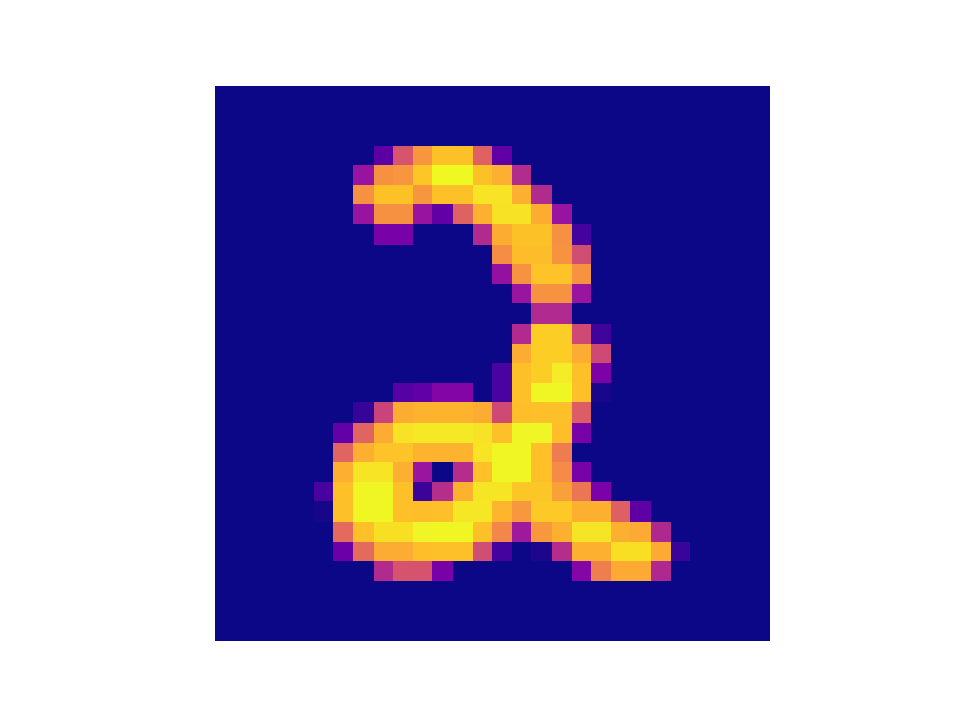
\includegraphics[width=1.0\textwidth]{figures/original.pdf}
    \end{minipage}%
    \begin{minipage}{0.04\linewidth}
        \centering
        \large $\ominus$
    \end{minipage}%
    \begin{minipage}{0.2\linewidth}
        \centering
        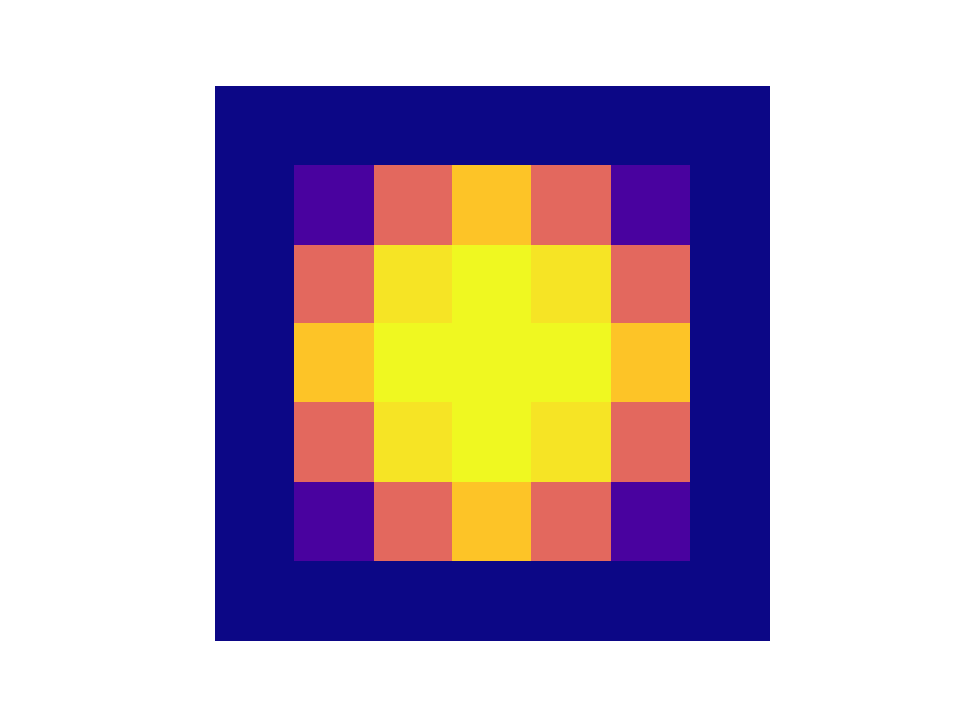
\includegraphics[width=0.7\linewidth]{figures/selem.pdf}
    \end{minipage}% 
    \begin{minipage}{0.06\linewidth}
        \centering
        \large $=$
    \end{minipage}%
    \begin{minipage}{0.3\linewidth}
        \centering
        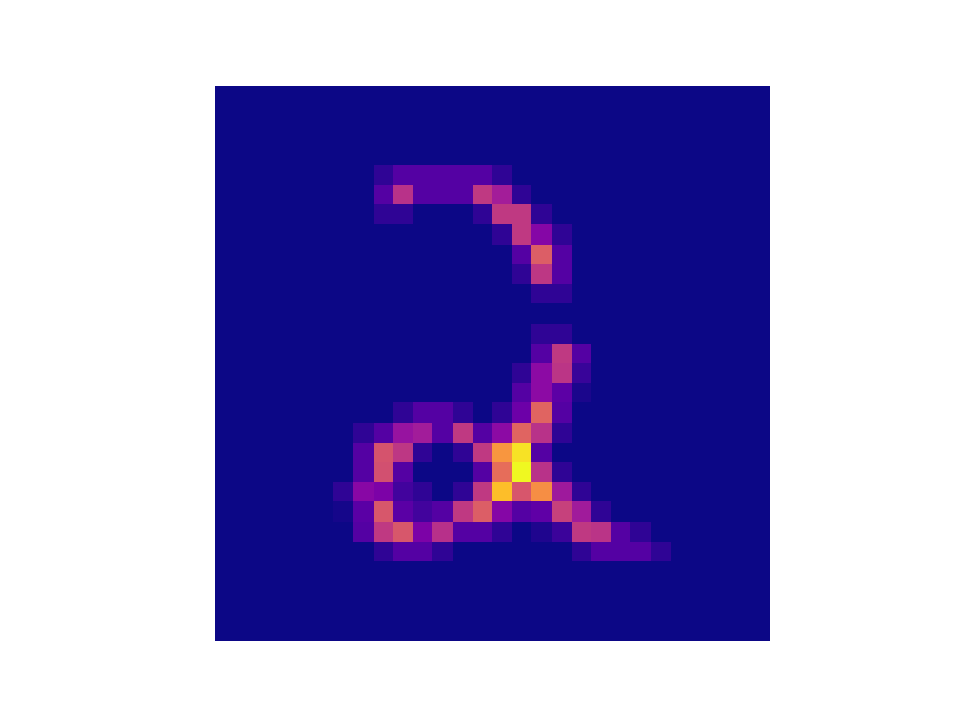
\includegraphics[width=1.0\textwidth]{figures/eroded.pdf}
    \end{minipage}
\end{minipage}%
\hfill%
\begin{minipage}{0.49\linewidth}
    \begin{minipage}{0.3\linewidth}
        \centering
        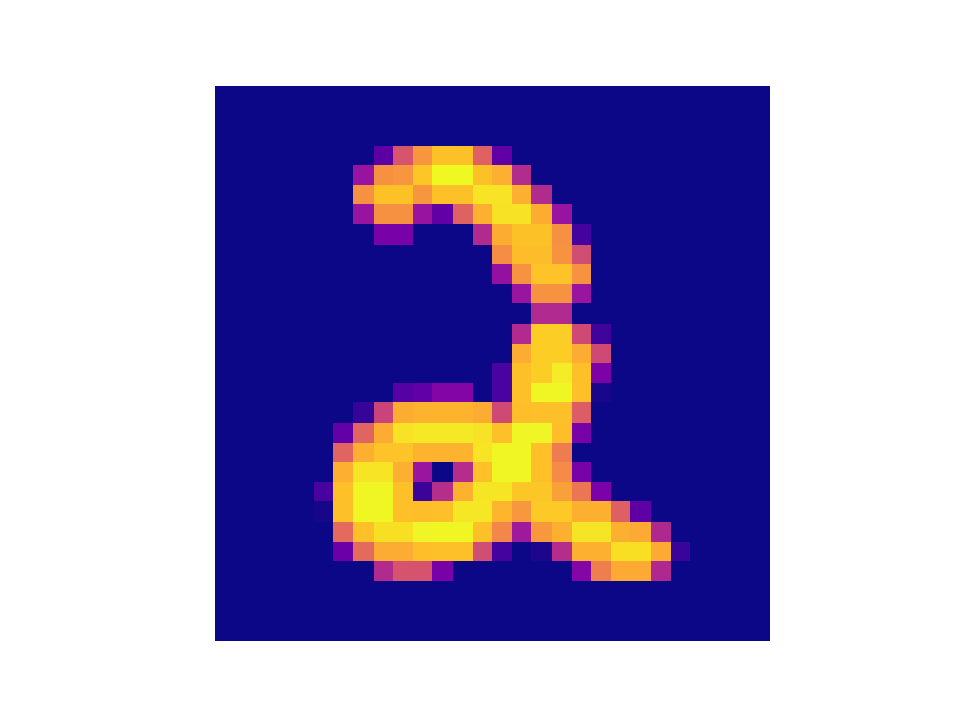
\includegraphics[width=1.0\textwidth]{figures/original.pdf}
    \end{minipage}%
    \begin{minipage}{0.04\linewidth}
        \centering
        \large $\oplus$
    \end{minipage}%
    \begin{minipage}{0.2\linewidth}
        \centering
        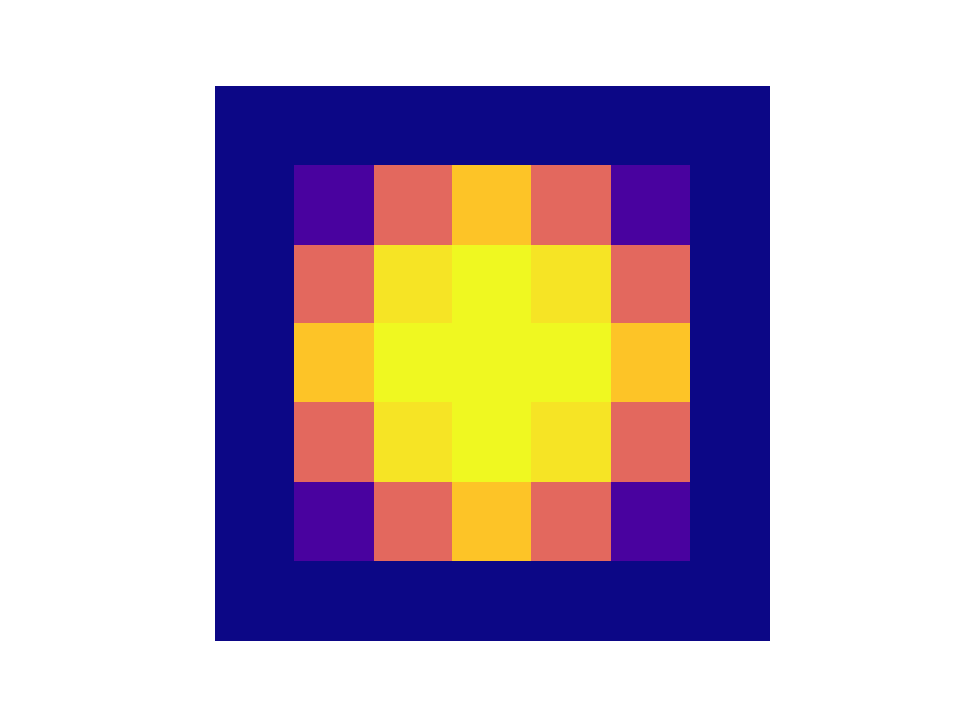
\includegraphics[width=0.7\linewidth]{figures/selem.pdf}
    \end{minipage}% 
    \begin{minipage}{0.06\linewidth}
        \centering
        \large $=$
    \end{minipage}%
    \begin{minipage}{0.3\linewidth}
        \centering
        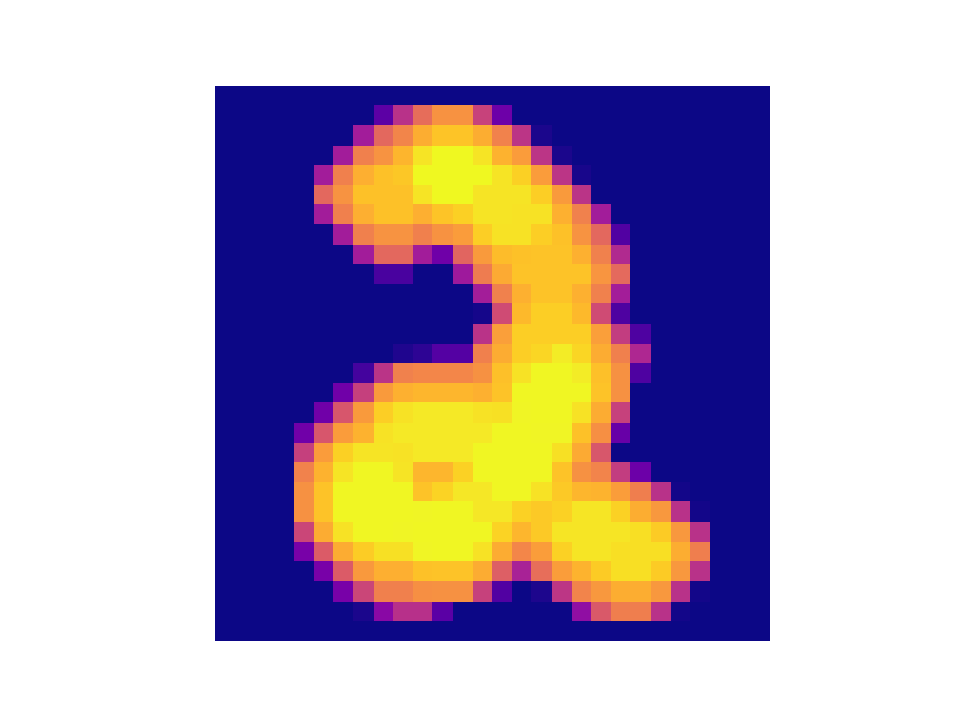
\includegraphics[width=1.0\textwidth]{figures/dilated.pdf}
    \end{minipage}
\end{minipage}%
    
    \caption{\centering Exemple d'une érosion $\ominus$ (à gauche) et d'une dilatation $\oplus$ (à droite) par une fonction structurante $B$ circulaire sur une image en niveaux de gris de la banque MNIST.}
    \label{fig:morpho_operations_example}
  \end{center}
\end{figure}

\vspace{-4mm}
La morphologie mathématique démontre une grande efficacité dans diverses applications de traitement d'images, telles que le débruitage et la détection d'objets \cite{Peters_1995, Horgan_1998}. Cependant, ces performances sont souvent tributaires du niveau d'expertise de l'utilisateur, ainsi que de sa capacité à déterminer la séquence appropriée des opérations fondamentales et à définir adéquatement les éléments structurants associés à la tâche en question. Par conséquent, l'automatisation de la définition des types d'opérations morphologiques et de leurs éléments structurants pour des applications spécifiques représente une perspective particulièrement séduisante. \\

\vspace{-2mm}
Récemment, plusieurs initiatives ont vu le jour en vue d'intégrer l'apprentissage automatique de séquences d'opérations morphologiques au sein des réseaux de neurones convolutionnels \cite{Masci_2012, Hermary_2022, Bloch_2021}. L'objectif est de remplacer les couches de convolution classiques par des couches morphologiques, capables d'apprendre et d'appliquer des érosions ou des dilatations. Les poids des filtres en jeu jouent alors un rôle analogue à celui des fonctions structurantes correspondantes.

%%% NEW PAGE %%%
\newpage

Cependant, en raison du caractère localement non différentiable des opérations morphologiques, qui reposent sur des minimas (érosion) ou maximas (dilatation) ensemblistes, des approches détournées doivent être mises en œuvre pour assurer une convergence optimale du réseau durant la phase d'apprentissage. Deux stratégies ont émergé dans la littérature : l'emploi d'approximations continues et différentiables des opérateurs de minimum et de maximum \cite{Masci_2012, Shih_2019, Kirszenberg_2021, Hermary_2022}, ou le traitement de la couche morphologique de manière similaire à la gestion des opérations localement non différentiables dans les architectures classiques (comme le max-pooling) \cite{Keiller_2019, Roy_2021}. \\

\vspace{-1.6mm}
Dans le cadre de l'emploi d'approximations différentiables du min et du max, la première couche morphologique fonctionnelle, la $p$Conv, a été proposée en 2012 en utilisant la formule de la moyenne contre-harmonique \cite{Masci_2012}. Plus récemment encore, ont été proposées dans \cite{Kirszenberg_2021}, et étendu dans \cite{Hermary_2022}, deux nouvelles couches morphologiques, la $\mathcal{L}$Morph et la $\mathcal{S}$Morph, qui reposent sur d'autres formules d'approximation. Ces couches sont capables d’apprendre de manière très performantes les opérations d’érosion, de dilatation, d'ouverture et de fermeture ainsi que l’élément structurant associé. Cependant, certaines propriétés de ces couches restent mal comprises, voire incomprises, en particulier dans les cas où l’apprentissage est un échec. \\

\vspace{-1.6mm}
L’objectif ici est donc d’explorer plus en profondeur le comportement de ces couches morphologiques différentiables, aussi bien sur des aspects théoriques (comportement asymptotique, morphologie de l'espace de la fonction de perte, convergence durant la phase d’apprentissage, impact de contraintes géométriques, etc.) que pratiques (analyse de la convergence des réseaux, des résultats d'apprentissage sous contrainte, de l'impact d'un partage de poids, etc.). Il s'agira en particulier d'apporter des solutions aux problèmes de convergence des réseaux associés. \\

\vspace{-1.6mm}
Dans leur article, R. Hermary et al. \cite{Hermary_2022} mettent en évidence de meilleures performances de convergence pour les couches $\mathcal{S}$Morph par rapport aux autres couches morphologiques existant. Les études et résultats dont ce rapport fait la synthèses seront ainsi focalisées sur ces couches-ci. Les solutions apportées pour améliorer la convergence des réseaux associés à ces couches, dits $\mathcal{S}$MorphNet, pourront aussi bien toucher la définition même des couches, que la structure des réseaux associés construits, ou que la définition de la fonction de perte lors de la phase d'entraînement. \\

\vspace{-1.6mm}
Dans un premier temps seront passées en revue les différentes méthodes de la littérature : la définition des opérateurs classiques de la morphologie mathématique, la structure des différentes couches morphologiques proposées existant, l'efficacité de convergence des réseaux correspondants vers la structure neuronale cible, ainsi que les différents cas d'échec persistants.
Dans un second temps seront présentées de manière théorique les différentes contributions apportées ainsi que les résultats pratiques de leur application, avant de comparer la convergence des réseaux améliorés à celle des réseaux existant de la littérature dans un dernier temps.

\newpage

%========================================================================================
%	2. ETAT DE L'ART
%========================================================================================

\section{État de l'art}

% Morphologie mathematique
\subsection{Morphologie mathématique} %Opérateurs classiques de la morphologie mathématique

\subsubsection{Morphologie binaire}
\vspace{0.2cm}
La morphologie mathématique a, en 1964, d'abord été introduite sous sa forme binaire \cite{Serra_1986}. Dans ce cadre, les images peuvent être définies soit de manière ensembliste, où elles et les objets contenus en elles sont définis comme des parties d'un ensemble E structuré comme un groupe pour l'addition, soit, par équivalence, de manière fonctionnelle booléenne, où les images sont définies comme fonctions sur un sous-ensemble de $E$ à valeurs dans $\{0,1\}$, où $1$ est associé aux objets et $0$ au fond de l'ensemble de définition \cite{Serra_1983}. Dans un contexte discret, tel que les images, on a $E=\mathbb{Z}^2$. \\

\vspace{-1.6mm}
Les opérations fondamentales de la morphologie mathématique sont l'érosion et la dilatation. Dans le cadre binaire, elles sont définies de manière ensembliste sur $E$. \\

\vspace{-1.6mm}
\noindent Soit $B \subset E$ l'élément structurant, servant de structure aux opérations morphologiques.

\noindent On définit $B_x$ comme l'ensemble $B$ translaté de $x \in E$ : \hspace{0.444cm} $B_x = \{ \, b+x \, \mid \, b \in B \, \}$

\noindent On définit $\breve{B}$ \hspace{0.7mm} comme l'ensemble symétrique de $B$ : \hspace{1.03cm} $\breve{B}$ \hspace{0.02mm} $= \{ \, -b \, \mid \, b \in B \, \}$

\vspace{0.4cm}
\begin{itemize}[leftmargin=*]
    \item[$\bullet$] L'érosion $\epsilon_B(X)$ d'une partie $X$ de $E$ par l'élément structurant $B$ est définie par : 
    \begin{equation}
        \epsilon_B(X) = X \ominus B = \{ \, x \, \mid \, B_x \subset X \, \}
        \label{binary_erosion}
    \end{equation}
\end{itemize}
\vspace{0cm}
\begin{itemize}[leftmargin=*]
    \item[$\bullet$] La dilatation $\delta_B(X)$ de $X$ par $B$ est, quant à elle, définie par : 
    \begin{equation}
        \delta_B(X) = X \oplus B = \{ \, x \, \mid \, \breve{B}_x \cap X \neq \emptyset \, \}
        \label{binary_dilation}
    \end{equation}
\end{itemize}

%figure
\vspace{-1.5mm}
\begin{figure}[ht]
  \begin{center}
      \subfigure[Image originale]{
          
\includegraphics[width=0.28\textwidth]{parts/2-etat_de_lart/A-operateurs_morphologiques_classiques/figures/BI_original.png}
          \label{fig:sub1}}\hfill
      \subfigure[Image érodée]{
          
\includegraphics[width=0.28\linewidth]{parts/2-etat_de_lart/A-operateurs_morphologiques_classiques/figures/BI_eroded.png}
          \label{fig:sub2}}\hfill
      \subfigure[Image dilatée]{
          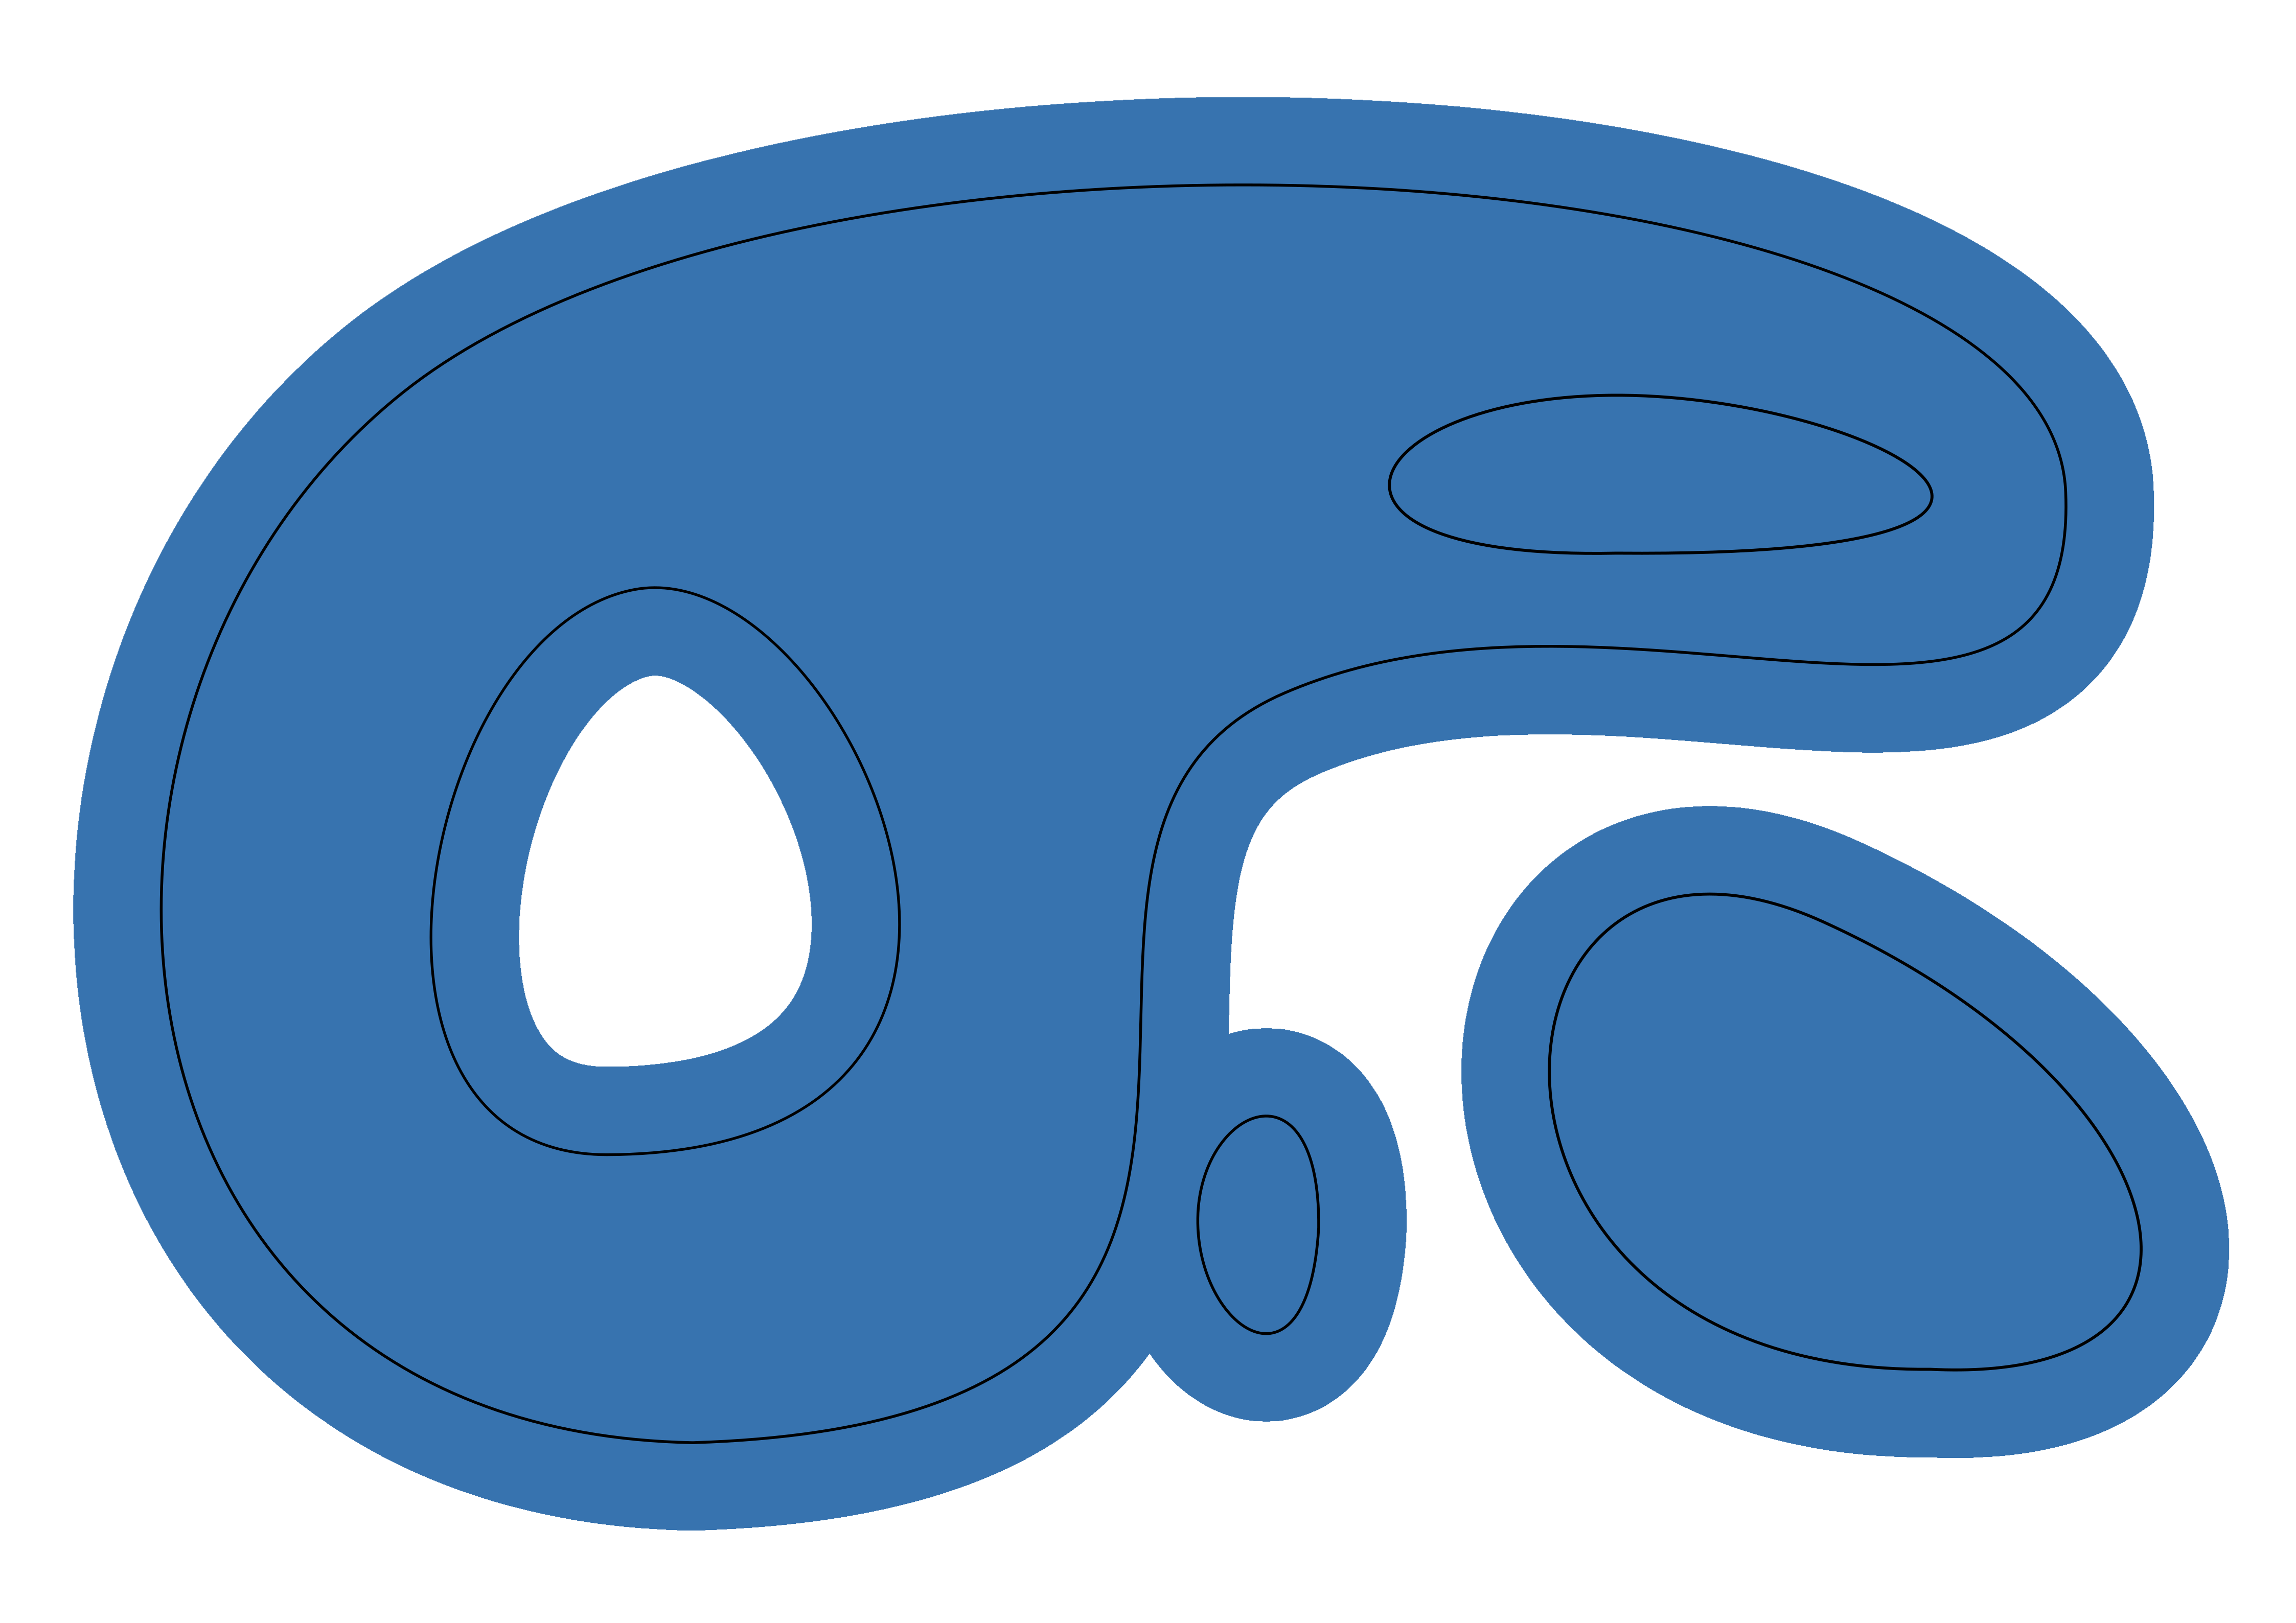
\includegraphics[width=0.28\textwidth]{parts/2-etat_de_lart/A-operateurs_morphologiques_classiques/figures/BI_dilated.png}
          \label{fig:sub3}}\hfill
      \subfigure[B]{
          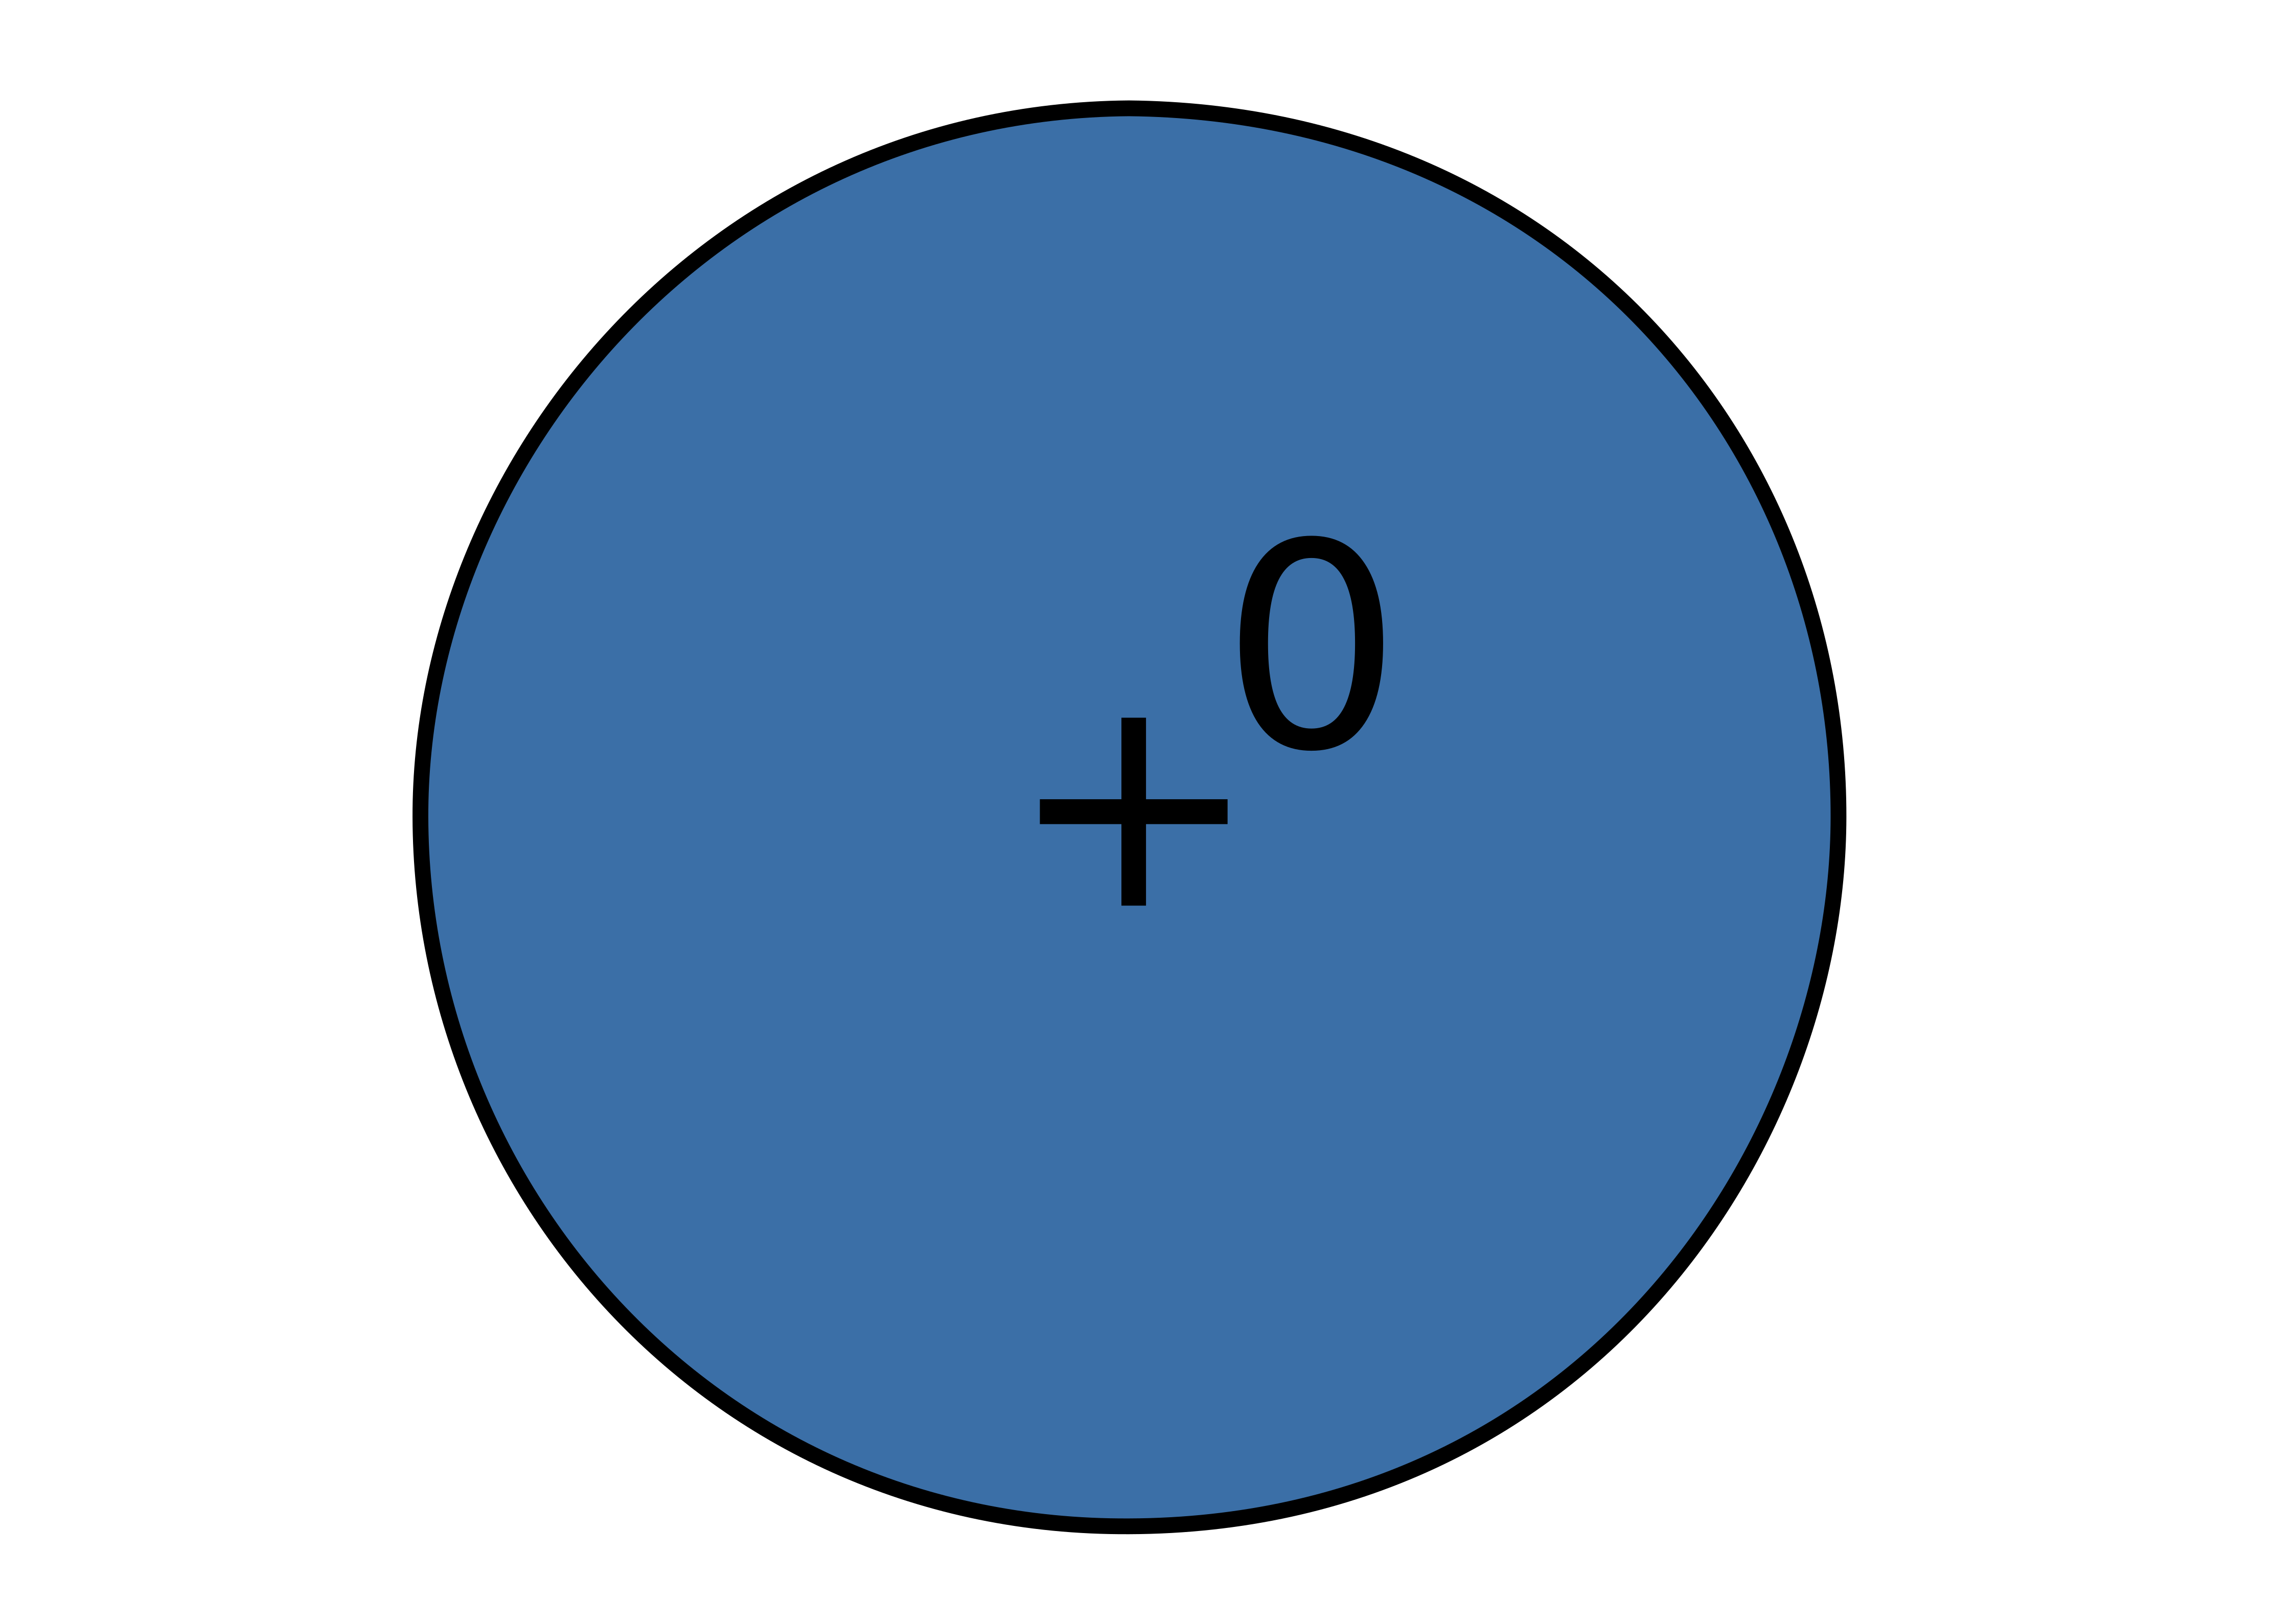
\includegraphics[width=0.05\textwidth]{parts/2-etat_de_lart/A-operateurs_morphologiques_classiques/figures/BI_selem.png}
          \label{fig:sub4}}
    \caption{ \centering Exemple de l'érosion $\ominus$ \ref{fig:sub2} et de la dilatation $\oplus$ \ref{fig:sub3} d'une image binaire \ref{fig:sub1} par un élément structurant binaire $B$ en forme de disque centré en $(0,0)$, fig. \ref{fig:sub4}.}
    \label{fig:morpho_binary_operations_example}
  \end{center}
\end{figure}

\vspace{-1.6mm}
En combinant l'érosion (\ref{binary_erosion}) et la dilatation (\ref{binary_dilation}), illustrées fig. \ref{fig:morpho_binary_operations_example}, on peut créer des opérations plus avancées, telles l'ouverture $\circ$ : $\gamma_B(X) = \delta_B(\epsilon_B(X))$ ; la fermeture $\bullet$ : $\phi_B(X) = \epsilon_B(\delta_B(X))$ ; ou encore le gradient morphologique : $\text{grad}_B(X)=\delta_B(X)-\epsilon_B(X)$.

\vfill

%%% ASPECT ENSEMBLISTE (on considère des sous-ensembles de Z²)
\newpage

\subsubsection{Morphologie en niveaux de gris}
\vspace{0.2cm}
La morphologie mathématique pour les images à niveaux a été développée après la morphologie binaire, dans le but de généraliser cette technique aux images fonctionnelles \cite{Haralick_1987, Serra_1992}. Dans ce cas plus général, les images et éléments structurants sont considérés comme des applications sur une partie de $E$ à valeurs dans une partie d'un autre ensemble tel que $\mathbb{Z}$ ou $\mathbb{R}$ pour les images à tons de gris, $\mathbb{Z}^3$ ou $\mathbb{R}^3$ pour les images en couleurs, ou tout autre ensemble construit comme groupe pour l'addition. \\

\vspace{-1.6mm}
Les opérations fondamentales de la morphologie mathématique sont l'érosion et la dilatation. On étudiera par la suite uniquement le cas des images à tons de gris. \\

\vspace{-1.6mm}
\noindent L'image fonctionnelle est notée $f: E \rightarrow G$. L'élément structurant est, comme l'image, une fonction notée $b: E \rightarrow G$, avec $G$ groupe pour l'addition ($\mathbb{Z}$ ou $\mathbb{R}$).

\vspace{0.4cm}
\begin{itemize}[leftmargin=*]
    \item[$\bullet$] L'érosion $\epsilon_b(f)$ de $f$ par $b$ est l'image $\epsilon_b(f) : E \rightarrow G$ définie pour tout $x \in E$ par : 
    \begin{equation}
        \epsilon_b(f)(x) = (f \ominus b)(x) = \min_{y \in E} \left \{ \, f(y) - b(y-x) \, \right \}
        \label{grey_erosion}
    \end{equation}
\end{itemize}
\vspace{0cm}
\begin{itemize}[leftmargin=*]
    \item[$\bullet$] La dilatation $\delta_b(f)$ de $f$ par $b$ est, quant à elle, l'image définie pour tout $x \in E$ par : 
    \begin{equation}
        \delta_b(f)(x) = (f \oplus b)(x) = \max_{y \in E} \left \{ \, f(y) + b(x-y) \, \right \}
        \label{grey_dilation}
    \end{equation}
\end{itemize}

\noindent Les processus d'érosion et de dilatation sont tous deux illustrés sur un exemple fig. \ref{fig:morpho_grey_operations_example}. \\

\vspace{-1.6mm}
On définit l'ouverture et la fermeture par les mêmes combinaisons entre l'érosion et la dilatation que dans la morphologie binaire. L'ouverture fonctionnelle $\circ$ est ainsi définie par : $\gamma_b(f) = \delta_b(\epsilon_b(f))$ ; et la fermeture fonctionnelle $\bullet$ par : $\phi_b(f) = \epsilon_b(\delta_b(f))$.  Il en est de même pour le gradient morphologique : $\text{grad}_b(f)=\delta_b(f)-\epsilon_b(f)$. \\

\vspace{-1.6mm}
Un lien direct entre la morphologie en niveaux de gris et la morphologie binaire peut se faire. Soit $B \subset E$ le support de l'élément structurant tel que défini dans la morphologie binaire. En définissant b comme fonction structurante plate telle que, pour tout $x \in E$ :

\vspace{-3.0mm}
\begin{center}
    $b(x) = \left \{    \begin{array}{rcl} 0 & \hspace{3.2mm} \text{si} \hspace{1.5mm} x \in B \\ -\infty & \text{sinon} \end{array}     \right.$  ,
\end{center}

\vspace{1.2mm}
\noindent les formules \ref{grey_erosion} et \ref{grey_dilation} permettent à la morphologie en niveaux de gris d'avoir le même comportement que la morphologie binaire, pour des images binaires définies comme fonctions sur E à valeurs dans $\{0,1\}$.

\vspace{2.5mm}
\noindent La formule de l'érosion devient alors : \hspace{4mm} $\epsilon_b(f)(x) = \min_{y \in B_{x}} \left \{ \, f(y) \, \right \}$

\noindent Et celle de la dilatation devient ainsi : \hspace{5mm} $\delta_b(f)(x) = \max_{y \in \breve{B}_{x}} \left \{ \, f(y) \, \right \}$

\vspace{2.5mm}
\noindent $\min_{y \in B_{x}} \left \{ \, f(y) \, \right \}$ correspond à l'inclusion de $B_x$ dans les objets de l'image $f$ au point $x$, et $\max_{y \in \breve{B}_{x}} \left \{ \, f(y) \, \right \}$ à la non vacuité de l'intersection entre $\breve{B}_x$ et les objets de $f$ en $x$.


\newpage

%figure
\vspace{2.0mm}
\begin{figure}[ht]
  \begin{center}
      \subfigure[Processus d'érosion évalué en un point $x$]{
          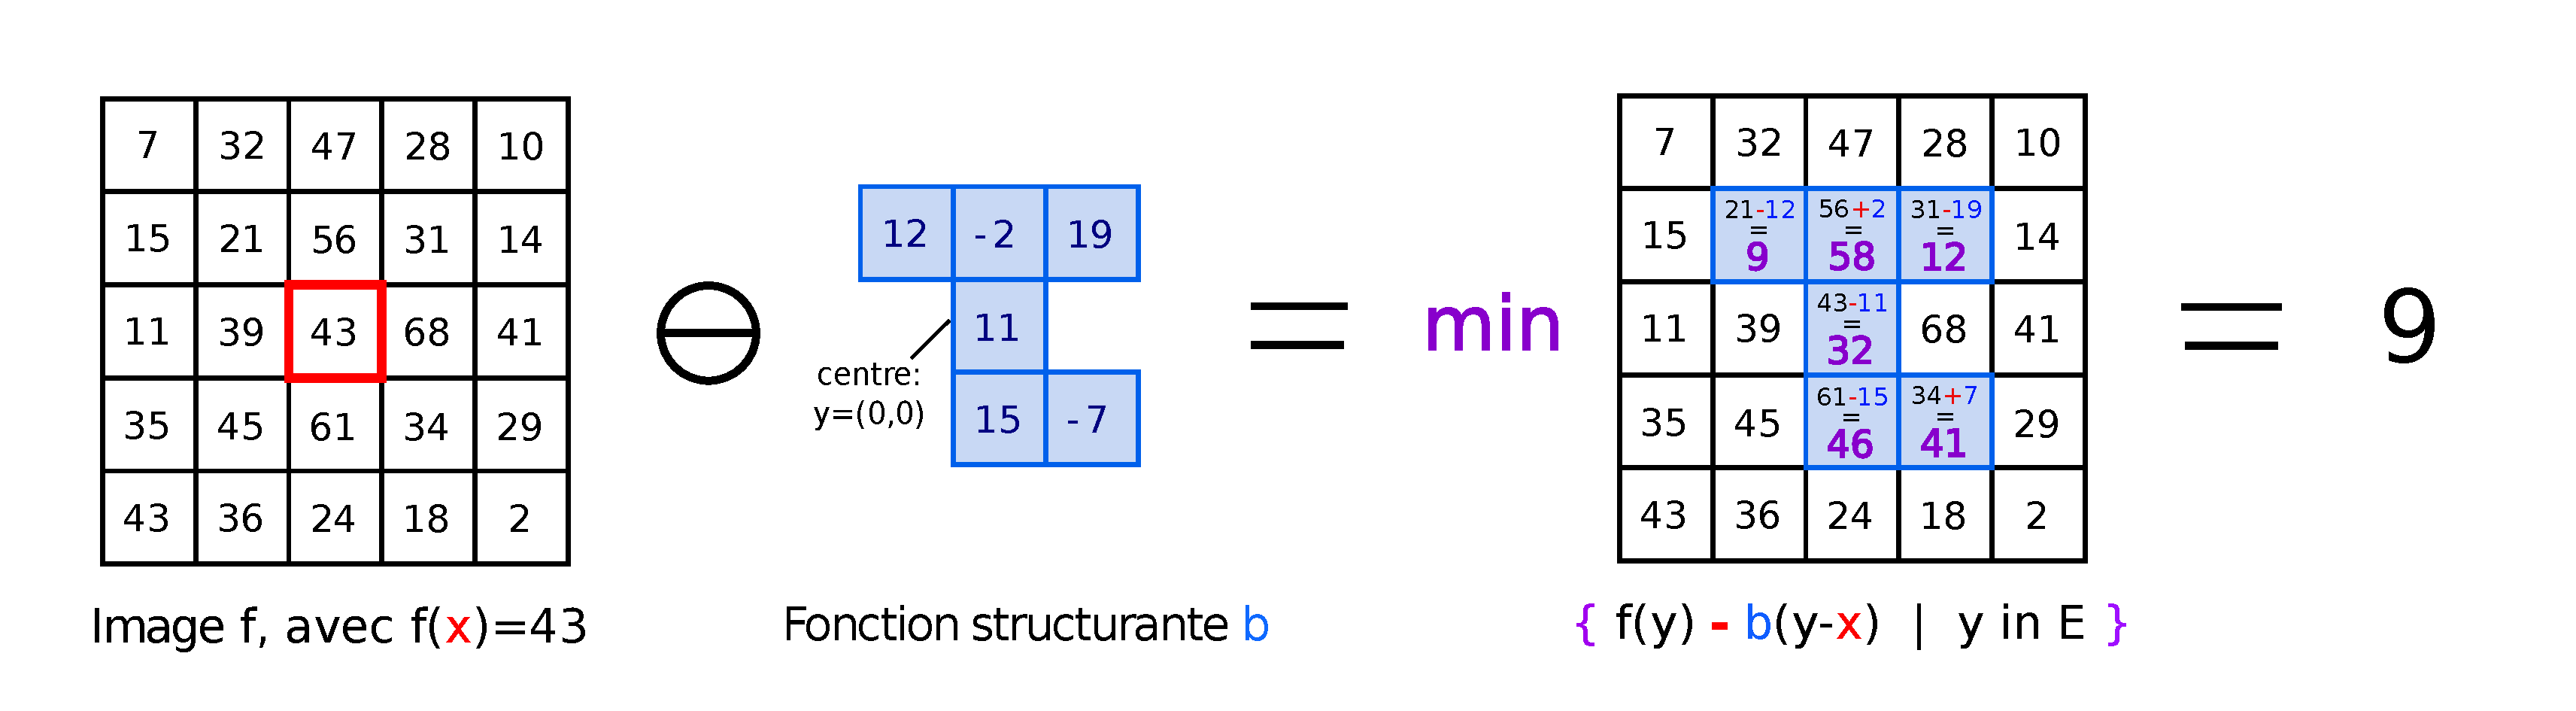
\includegraphics[width=1.00\textwidth]{parts/2-etat_de_lart/A-operateurs_morphologiques_classiques/figures/grey_erosion.pdf}
          \label{fig:sus1}}\hfill
      \subfigure[Processus de dilatation évalué au même point $x$]{
          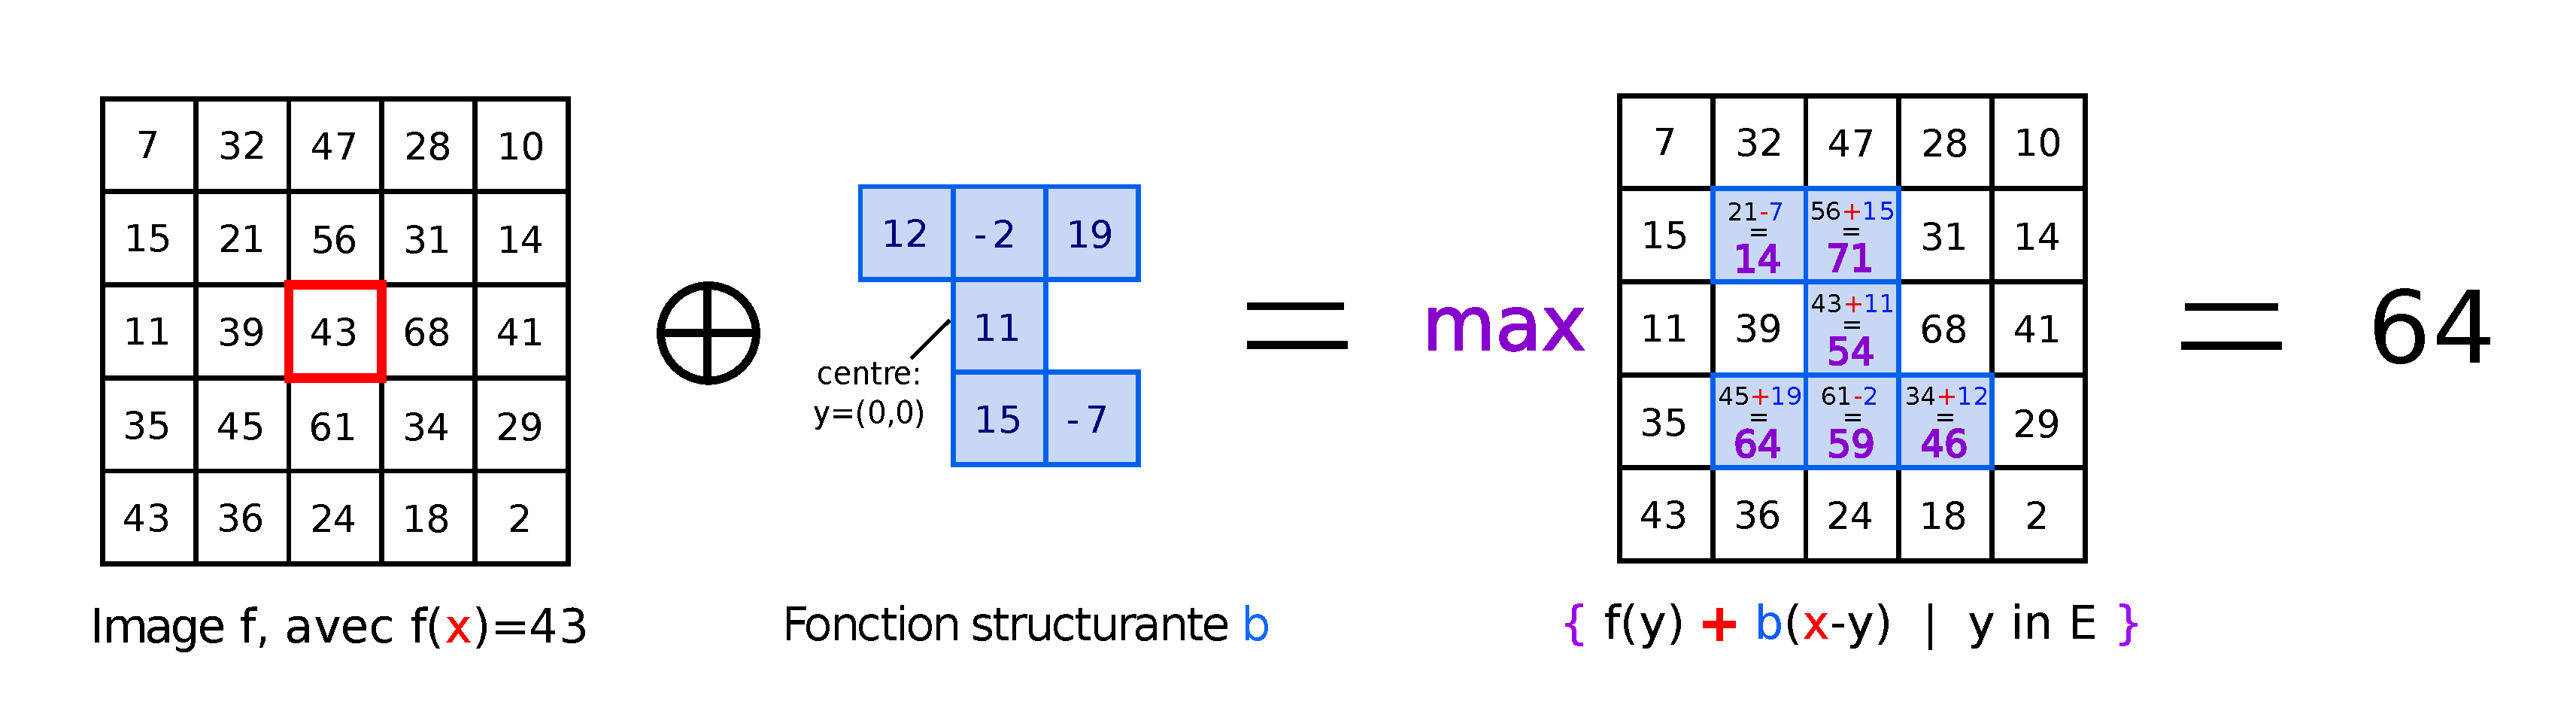
\includegraphics[width=1.00\linewidth]{parts/2-etat_de_lart/A-operateurs_morphologiques_classiques/figures/grey_dilation.pdf}
          \label{fig:sus2}}
    \caption{ \centering Exemple du processus de l'érosion $\ominus$ \ref{fig:sus1} et de celui de la dilatation $\oplus$ \ref{fig:sus2} sur une image $f$ en niveaux de gris, en un point $x \in \mathbb{Z}^2$, et par un élément structurant $b$.}
    \label{fig:morpho_grey_operations_example}
  \end{center}
\end{figure}

\vspace{1.0mm}
\noindent \textbf{Remarque pour la suite :} \\

\vspace{-0.6mm}
En morphologie mathématique, que ce soit en binaire ou en niveau de gris, la dilatation considère la symétrie $\breve{b}=-b$ de l'élément structurant $b$, contrairement à l'érosion qui considère simplement $b$ \cite{Haralick_1987}. En niveaux de gris, cela est illustré par l'inversion de $x$ avec $y$, en argument de l'élément structurant $b$, entre l'érosion et la dilatation. Voir les formules précédentes, ainsi que l'illustration fig. \ref{fig:morpho_grey_operations_example}. Il s'agit d'un élément important dans la suite de ce rapport, où les différentes formules d'appriximation de ces opérations morphologiques considèrent soit uniquement $b$ soit uniquement sa symétrique $\breve{b}$ pour ces deux opérations à la fois, afin de conserver la continuité des formules lors du passage d'un effet d'érosion à un effet de dilatation, et inversement. \\

\vspace{-1.6mm}
\noindent De plus, dans la morphologie en niveaux de gris, la seconde différence de construction entre l'ensemble affecté au min de l'érosion et celui affecté au max de la dilatation, est le signe devant l'élément structurant $b$. Voir formules associées \ref{grey_erosion} et \ref{grey_dilation}. Cette seconde différence joue également un rôle important pour la suite, dans la définition des formules d'approximation de ces opérateurs morphologiques. 

\vfill

%%% ASPECT FONCTIONNEL (on considère des fonctions d'un sous-ensemble de Z² dans un sous-ensemble d'un autre groupe, genre R ou Z)
\newpage

% Structure des reseaux
\subsection{Structure des réseaux morphologiques} %Construction et structure des réseaux morphologiques

\subsubsection{Construction d'une couche morphologique}
\vspace{0.2cm}
La principale motivation dans le développement de couches morphologiques, initié à la fin des années 1980 \cite{Wilson_1989, Davidson_1990}, est l'intégration d'opérateurs morphologiques automatiques, capables d’apprendre et d’appliquer des érosions ou des dilatations sur des images données, au sein même des réseaux de neurones convolutionnels \cite{LeCun_2015}, en remplacement des couches de convolution classiques dans ces réseaux-ci. \\

\vspace{-1.4mm}
Ces nouvelles couches jouent ainsi, comme pour les couches classiques, le rôle de \textit{filtres} appliqués aux images en entrée du réseau, dont le noyau à poids variables est de taille constante, mais qui sont ici régis par une fonction particulière d'approximation de l'érosion et de la dilatation (approximation lisse nécessaire due à la non-dérivabilité du min et du max des opérations d'érosion et de dilatation). Le noyau de ces couches morphologiques joue alors un rôle analogue à celui des fonctions structurantes correspondantes, dont il cherche à imiter le comportement \cite{Bloch_2021}. Un réseau de neurones composé de telles couches est ainsi appelé << réseau de neurones morphologique >>. \\

\vspace{-1.4mm}
Soit $f: I \subseteq E \rightarrow \mathbb{R}$ une image, fonction sur une partie dénombrable $I$ de $E$ à valeurs dans $\mathbb{R}$, et soit $w: W \subseteq E \rightarrow \mathbb{R}$ le noyau d'une couche morphologique, également défini sur une partie dénombrable $W$ de $E$. Comme précédemment, on écrit $\breve{W}_x$ pour désigner l'ensemble symétrique de $W$ translaté de $x \in E$ :   $\breve{W}_x = \{ \, -\text{w} + x \, \mid \, \text{w} \in W \, \}$. \\

\vspace{-1.4mm}
\noindent \textbf{Attention} : Ici, nous parlons de << noyau >> ou de << filtre >> d'une couche pour désigner la fonction $w$ associée telle que définie ci-dessus et qui renvoie les poids $(w_y)_{y \in W} \in \mathbb{R}^{|W|}$ variables du filtre sur le support $W \subseteq E$. La << couche morphologique >>, quant à elle, est l'objet contenant à la fois ce noyau $w$ ainsi qu'une fonction de transformation $T$, qui prend en argument $w$ et qui, à partir d'une image $f$ en entrée de couche, renvoie une nouvelle image (également application de $I$ dans $\mathbb{R}$) en fonction de $f$ et $w$. \\


\vspace{-1.6mm}
\noindent D'une manière générale, la fonction de transformation $T$ peut être décomposée en deux étapes de transformations, l’une s'inscrivant dans l’autre. La première, locale, considère $f$ et $w$ localement en produisant, pour un point $x \in I$ donné, des \textit{familles de réels} à travers la mise en relation de la valeur $f(y)$ en $y \in \breve{W}_x$ avec la valeur $w(x-y)$ au point $x-y$ symétrique de $x+y$ par rapport à $x$. La seconde étape, plus globale, met en relation, pour ce même $x \in I$, l'ensemble des éléments de ces \textit{familles de réels} produites. Elle renvoie alors la valeur en ce point $x$ associée à la nouvelle image. Voir fig. \ref{fig:structure_couche_morpho}. \\

\vspace{-1.6mm}
\noindent Par exemple, pour une couche de convolution classique, la relation locale $\text{R}_\text{l}$ entre les $f(y)$ et $w(x-y)$ est le produit ($\times$), et la relation globale $\text{R}_\text{g}$ entre les éléments de la famille de réels produite est l'addition sur $y \in \breve{W}_x$. La nouvelle image $f_c$ issue de cette transformation $T$ est ainsi définie pour tout $x \in I$ par : $f_c(x) = \sum_{y \in \breve{W}_x} f(y) w(x-y)$. Pour une dilatation classique, $\text{R}_\text{l}$ est la somme (+), et $\text{R}_\text{g}$ est l'opération de maximum.
%D'une manière générale et plus informelle, la fonction de transformation $T$ d’une couche morphologique peut être décomposée en deux couches de transformation, qui s’imbriquent l’une dans l’autre. La première considère $f$ et $w$ de manière locale, et produit des familles de réels, pour un point variable $x$ donné, à travers la mise en relation de la valeur $f(y)$ de l'image $f$ en un pixel $y \in I$ avec la valeur $w(x-y)$ du noyau $w$ au pixel $x-y$ symétrique à $y$ par rapport à $x$, et ce pour tout $y \in \breve{W}_x$ créant ainsi une famille de réels indexée par $y \in \breve{W}_x$, et ce pour une ou plusieurs relations considérées. La seconde couche, plus globale, produit, à partir des éléments de ces familles de réels issus des relations entre $f(y)$ et $w(x-y)$ considérées pour un certain $x \in I$, la valeur au point $x$ associée à la nouvelle image. 
%Les relations locales entre les $f(y)$ et $w(x-y)$ n'apparaît pas explicitement dans la formule générale de $T$, mais deviennent explicites dans les différentes formules explicitées de $T$.



\newpage

% graphics
\begin{figure}[ht]
  \begin{center}
    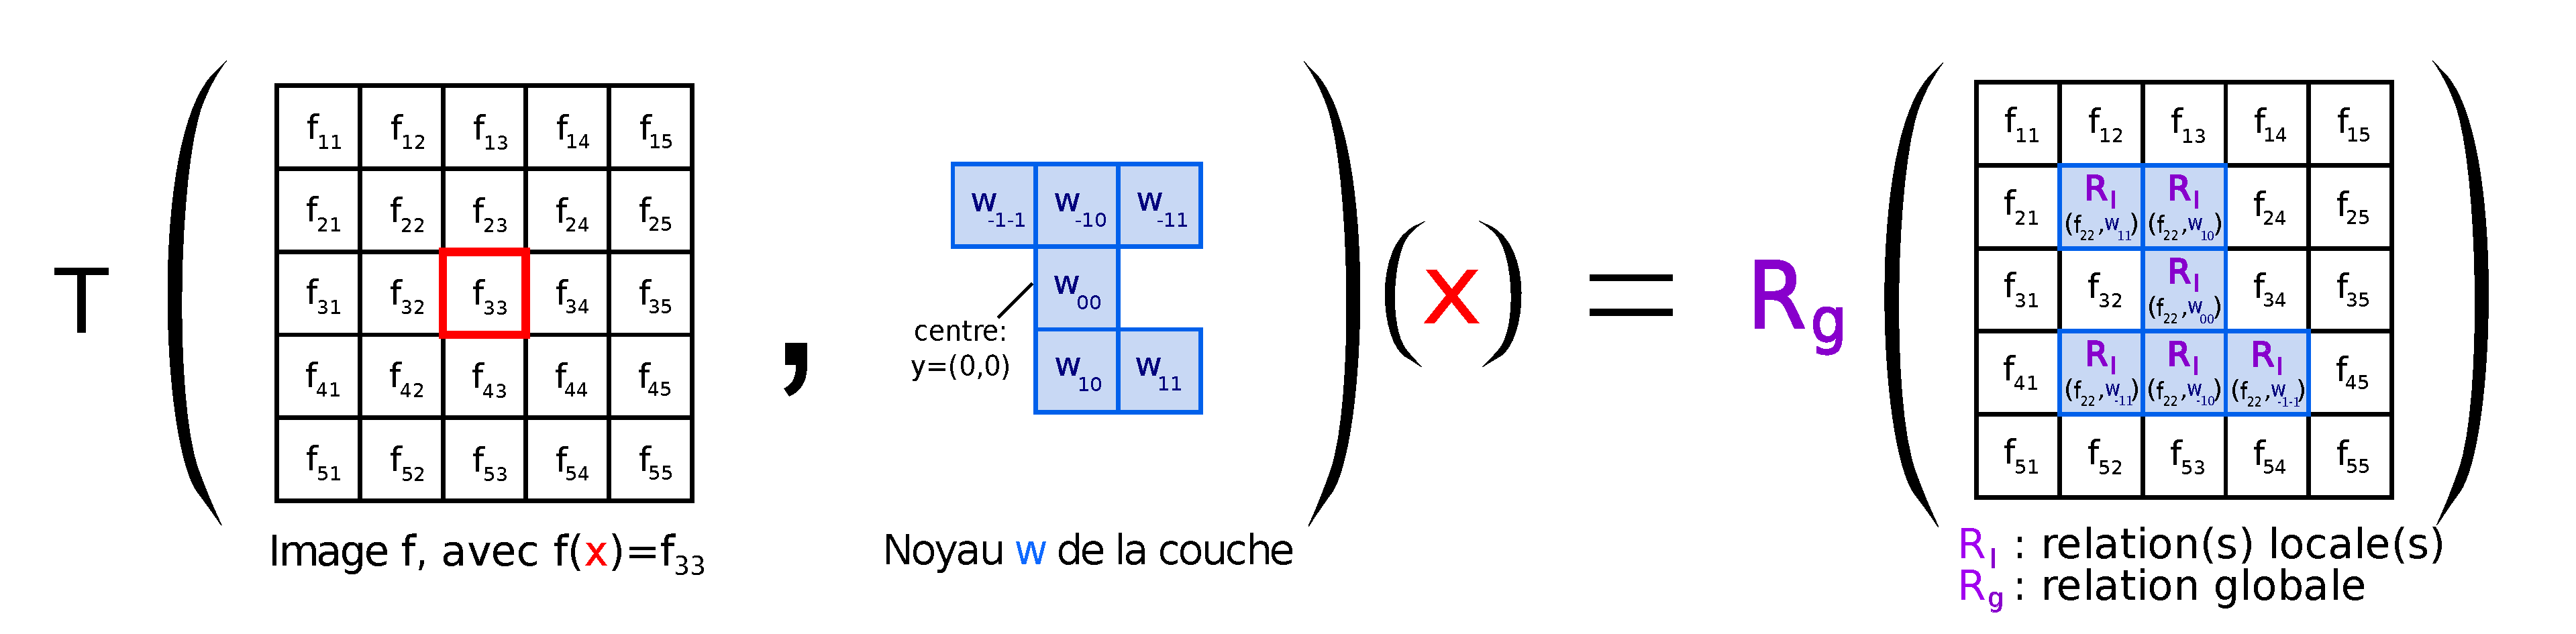
\includegraphics[width=1.00\textwidth]{parts/2-etat_de_lart/B-structure_des_reseaux_morphologiques/figures/couche_morpho.pdf}
    \caption{ \centering Illustration de la décomposition de la fonction de transformation $T$ en relations locales $R_l$ et une globale $R_g$, sur une image $f$ avec le noyau $w$ et au point $x$.}
    \label{fig:structure_couche_morpho}
  \end{center}
\end{figure}

\vspace{-1.8mm}
\noindent La fonction $T$ renvoie l'image $T(f,w)$ définie sur $I$ dans $\mathbb{R}$. On écrira cette nouvelle image, sans expliciter les relations locales $\text{R}_\text{l}$ entre les $f(y)$ et $w(x-y)$ ou globale $\text{R}_\text{g}$, simplement comme suit :
\vspace{-2.6mm}
\begin{align*}
T(f,w) \colon I & \longrightarrow \mathbb{R}\\
x & \longmapsto T \left ( f, w \right ) (x)
\end{align*}

\vspace{1.0mm}
\noindent La fonction de transformation $T$, qui prend en argument le couple image-noyau $(f,w)$, transforme ainsi l'image $f$, en entrée de la couche, en une nouvelle image de même taille, en considérant, pour chacun des pixels $x$ appartenant au support $I$ de l'image d'entrée, le voisinage défini par le support $W \subseteq E$ du noyau $w$ (illustration fig. \ref{fig:structure_couche_morpho}). \\

La bonne définition d'une telle fonction de tranformation $T$ au sein d'une couche permettrait d'appliquer à l'image $f$ l'effet désiré (convolution, max-pooling, morphologie, etc.), avec les poids du noyau $w$ de la couche en question, grâce à des mises en relation locales entre $f(y)$ et $w(x-y)$ et à une relation globale sur toutes ces dernières. \\

\vspace{-1.6mm}
\noindent Dans le cadre des réseaux de neurones, on va définir ces différentes relations de sorte que la fonction $T$ soit \textit{continue} et \textit{dérivable} localement partout par rapport aux poids $(w_y)_{y \in W}$ variables du noyau $w$, afin de pouvoir calculer le gradient du réseau lors de la phase d'apprentissage et mettre à jour ces poids par rétropropagation du gradient. \\

Le but ici, dans le cadre des couches morphologiques, est alors de trouver une fonction dérivable $T$ (et donc de définir les différentes relations locales et globale telles que décrites ci-dessus) adaptée, pour approximer au mieux l'effet des deux opérateurs morphologiques fondamentaux, l'érosion et la dilatation, et ce en une \textit{unique} formule. \\

\vspace{-1.6mm}
\noindent Ici, les noyaux des couches morphologiques seront toujours accompagnés d'un poids supplémentaire, noté $p$ ou $\alpha$, qui est indépendant des poids du noyau-même, et dont le rôle sera de faire une transition continue lisse entre le comportement d'érosion et celui de dilatation de la couche morphologique \cite{Hermary_2022}. Pour mieux distinguer ce poids des autres, on notera la nouvelle image de $T$: $T(f,w,p)$. Les différentes définitions de la fonction de transformation $T$ et l'intégration du poids $p$ sont explicitées partie 2.3.

\newpage

\subsubsection{Architecture d'un réseau morphologique}
\vspace{0.2cm}
Les couches morphologiques, telles que décrites précédemment, sont intégrées dans les réseaux de neurones morphologiques de la même manière que les couches de convolution dans les réseaux de neurones convolutionnels \cite{Hassoun_1996}. Dans le cadre de ce travail, nous construisons des réseaux comportant uniquement une ou plusieurs couches morphologiques successives, et pouvant comporter en plus (ou non) des couches de rééchelonnage de l'image, constantes ou avec des poids variables appris par le réseau lors de la phase d'entraînement, telles qu'une couche de convolution de taille 1 \cite{Keiller_2019, Bloch_2021}. \\

\vspace{-0.6mm}
\noindent Dans un tel réseau morphologique :
\vspace{0.8mm}
\begin{itemize}%[leftmargin=*]
    \item[$\bullet$] l'entrée est une matrice 3D représentant un ensemble d'images 2D en niveaux de gris définies sur une partie $I$ de $\mathbb{Z}^2$, de taille $n \times l \times h$, avec $n$ le nombre d'images, $l$ la longueur verticale des images et $h$ leur hauteur ;
    \vspace{0.4mm}
    \item[$\bullet$] les images sont filtrées successivement par les différentes couches du réseau, à travers une succession ordonnées de couches morphologiques et de couches de rééchelonnage si incluses dans le réseau ;
    \vspace{0.4mm}
    \item[$\bullet$] la sortie est une matrice 3D représentant l'ensemble des $n$ images 2D filtrées, de même taille $n \times l \times h$ que la matrice d'entrée. \\
\end{itemize}

\vspace{-1.0mm}
Le nombre de couches morphologiques à intégrer dans ces réseaux dépend de l'opération que l'on souhaite simuler ou du contexte dans lequel ils s'inscrivent. \\

\vspace{-1.6mm}
\noindent Typiquement, pour des opérations d'érosion ou de dilatation, le réseau comportera une unique couche morphologique, accompagnée ou non de couches de rééchelonnage. Pour des opérations d'ouverture (érosion suivie de dilatation) ou de fermeture (dilatation suivie d'érosion), chaque couche morphologique ne pouvant simuler le comportement que de l'une des deux opérations morphologiques fondamentales, le réseau comportera deux couches morphologiques successives, dans le but que l'une simule le comportement d'une érosion, et que l'autre simule celui de l'érosion. Pour une opération de dessalage (i.e. supprimer les bruits poivre et sel sur les images), on voudra intégrer quatre couches morphologiques successives, pour tenter d'imiter le comportement d'une ouverture suivie d'une fermeture, ou inversement. \\

\vspace{-1.6mm}
\noindent Il sera également possible de construire des réseaux comportant plusieurs couches morphologiques, dans le cadre d'une simple opération d'érosion ou de dilatation, afin de mieux comprendre leur fonctionnement et d'étudier le comportement et la convergence de ces réseaux durant la phase d'apprentissage. Un des points d'intérêt est l'étude de la forme que les noyaux adopteront pour décomposer en plusieurs parties une opération qu'une seule couche suffit à simuler. A l'inverse, il pourra être également pertinent d'étudier le comportement de réseaux composés d'une seule couche, pour des opérations plus complexes que l'érosion ou la dilatation.


\newpage

% figure
\begin{figure}[ht]
  \begin{center}
    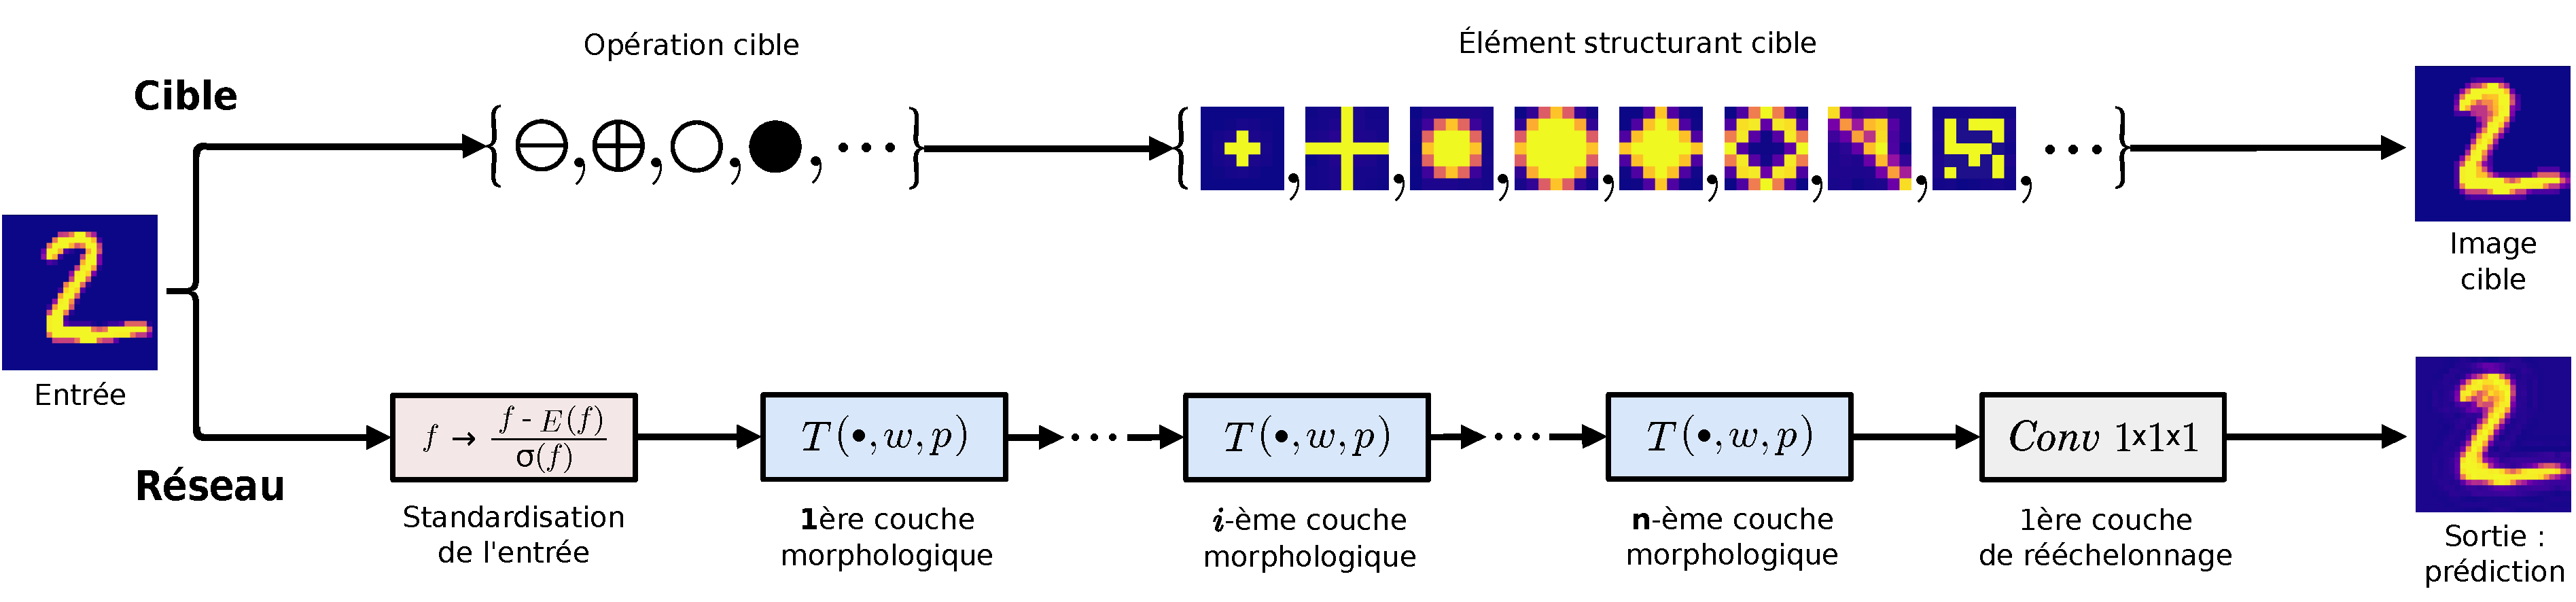
\includegraphics[width=1.00\textwidth]{parts/2-etat_de_lart/B-structure_des_reseaux_morphologiques/figures/reseau_morpho.pdf}
    \vspace{-3.6mm}
    \caption{ \centering Illustration de l'architecture type des réseaux de neurones morphologiques. Cas où l'opération et l'élément structurant cibles sont définis.}
    \label{fig:architecture_reseau_morpho}
  \end{center}
\end{figure}

\vspace{-3.4mm}
De plus, l'intégration ou non de couches de rééchelonnage des valeurs des images dépend des besoins et du comportement de convergence du réseau. Un filtre de rééchelonnage peut être linéaire (normalisation linéaire dans un intervalle $[a,b]$, standardisation, etc.) ou de forme plus complexe (logarithmique, tangente hyperbolique, etc.), et peut être constant (fonction déterministe invariante) ou comportant des poids variables appris par le réseaux lors de l'apprentissage. Dans ce dernier cas, les filtres linéaires sont typiquement de la forme : $f \rightarrow f \times s + b$, avec $s$ l'échelle (<< scale >>) et $b$ le biais (<< bias >>), tous deux formant les deux poids de cette couche de rééchelonnage. Il s'agit donc d'une couche de convolution classique, de taille $1 \times 1 \times 1$. \\

\vspace{-2.2mm}
%Pour des raisons d'amélioration de la convergence, plusieurs opérations intermédiaires, en entrée du réseau, entre les couches morphologiques, ou en sortie du réseau, peuvent être faites sur les images. En particulier, 
Hermary et al. \cite{Hermary_2022} ont montré que l'ajout d'un filtre de standardisation des images en entrée du réseau, accompagnée d'une couche de rééchelonnage linéaire de l'image (convolution) en sortie de ce dernier, permet une meilleure convergence lors de la phase d'apprentissage. 
Ainsi, l'architecture type des réseaux de neurones morphologiques qu'on utilisera est illustrée fig \ref{fig:architecture_reseau_morpho}. Elle définit d'abord un filtre de standardisation des images, puis $n$ couches morphologiques successives, pour finir avec une couche de convolution de taille 1 pour rééchelonner l'image en sortie. L'illustration montre le cas où l'opération et l'élément structurant cibles sont définis. Mais ils peuvent ne pas l'être, comme dans le cas du dessalage, où l'on considère simplement des images cibles vers lesquelles les prédictions du réseau cherchent à converger. \\

\vspace{-2.2mm}
A noter que le réseau construit n'est informé ni de l'opération cible, ni de l'élément structurant cible. Le réseau converge librement et se met à jour uniquement par rapport à l'image de sortie cible ; les poids (les $w_i$ du noyau $w$ et le paramètre de contrôle $p/\alpha$) des couches morphologiques et ceux des couches de rééchelonnage se mettant à jour sur la base de l'erreur (MSE) entre l'image cible et l'image prédite par le réseau. Ainsi, les couches morphologiques ne convergent pas nécessairement vers l'état espéré, et chacun n'adopte pas forcément un comportement morphologique (soit érosion ou soit dilatation) tel que souhaité, dû au lissage continue obligatoire de la transition entre un comportement d'érosion ou de dilatation de la couche. Là est tout l'enjeu d'une bonne définition de la fonction de transformation $T$ des couches et de l'analyse du comportement et de la convergence des réseaux construits.

\newpage

% Couches morphologiques existantes
\subsection{Les différentes couches morphologiques} %Couches morphologiques existant

\subsubsection{Couche \textit{p}-convolution}
\vspace{0.2cm}
La toute première couche morphologique a été introduite par Masci et al. \cite{Masci_2012} suite aux travaux de Angulo et al. \cite{Angulo_2010}. Il s'agit de la couche $p$-convolution. Dans une telle couche, l'approximation, qui définie $T$, des opérations d'érosion et de dilatation se base sur la moyenne contre-harmonique (CHM), également dite de Lehmer \cite{Bullen_1987}. \\

\vspace{-1.8mm}
\noindent La CHM du vecteur $\textbf{x} = (x_1,...,x_n) \in (\mathbb{R}_+)^n$ pondéré par $\textbf{w} = (w_1,...,w_n) \in (\mathbb{R}_+)^n$ et d'ordre $p \in \mathbb{R}$ est : %définie par :

\vspace{-5mm}
\begin{equation}
    CHM(\textbf{x},\textbf{w},p) = \frac{\sum_{i=1}^n w_ix_i^p}{\sum_{i=1}^n w_ix_i^{p-1}}
    \label{CHM}
\end{equation}

\vspace{2mm}
%Pour $p = 0$ (resp. $p = 1$), la moyenne de Lehmer $CHM(\textbf{x},\textbf{w},p)$ correspond à la moyenne harmonique pondérée (resp. moyenne arithmétique pondérée). Elle correspond à la moyenne contraharmonique lorsque $p = 2$ et $\textbf{w} = 1$ (toutes les coordonnées de \textbf{w} étant égales à $1$). 
\noindent Étant donné que les vecteurs \textbf{x} et \textbf{w} ont des coordonnées positives, c'est le maximum (resp. minimum) des coordonnées de \textbf{x} qui domine le numérateur et le dénominateur de l'équation \ref{CHM} lorsque $p$ tend vers $+\infty$ (resp. $-\infty$). On a ainsi aux limites : %Comportement asymptotique :

\vspace{2.6mm}
\noindent\begin{minipage}{.5\linewidth}
    \begin{equation*} 
        \lim_{p \rightarrow -\infty} CHM(\textbf{x},\textbf{w},p) = \min_{i \in \llbracket 1,n \rrbracket} x_i 
    \end{equation*}
\end{minipage}%
\begin{minipage}{.5\linewidth}
    \begin{equation*} 
        \lim_{p \rightarrow +\infty} CHM(\textbf{x},\textbf{w},p) = \max_{i \in \llbracket 1,n \rrbracket} x_i 
    \end{equation*}
\end{minipage}

\vspace{4mm}
%\noindent Ainsi, la CHM permet également des approximations douces des opérations de minimum et de maximum pour de grandes valeurs négatives et positives de p. \\

%\vspace{-1.4mm}
La formule de la $p$-convolution se base sur celle de la CHM afin d'avoir le même comportement asymptotique que ce dernier en minimum ou maximum des coordonnées de \textbf{x}. La $p$-convolution $p\text{Conv}(f,w,p)$ d'une image $f: I \subseteq \mathbb{Z}^2 \rightarrow \mathbb{R}_+$ au pixel $x \in I$ avec un noyau de convolution positif $w: W \subseteq \mathbb{Z}^2 \rightarrow \mathbb{R}_+$ et avec $p \in \mathbb{R}$ est définie par :

\vspace{0.5mm}
\begin{equation}
    \pmb{p}\textbf{Conv} (f,w,p)(x) = (f *_p w)(x) = \frac{\sum_{y \in \breve{W}_x} f(y)^p w(x-y)}{\sum_{y \in \breve{W}_x} f(y)^{p-1} w(x-y)}
    \label{pConv}
\end{equation}

\vspace{4mm}
\noindent L'étude des propriétés asymptotyques de la $p$Conv a notamment été faite par Jesús Angulo et al. \cite{Angulo_2010}, qui montrent qu'aux limites de $p$, la $p$Conv se comporte ainsi :

\vspace{-0.4mm}
\begin{equation*} 
    (f *_p w)(x) \underset{p \to -\infty}{\longrightarrow} \min_{y \in \breve{W}_x} \left \{ f(y) - \frac{1}{p} \log{(w(x-y))} \right \} = \left ( f \ominus \frac{1}{p} \log{ (\breve{w}) } \right )(x)
\end{equation*} 
\begin{equation*} 
    (f *_p w)(x) \underset{p \to +\infty}{\longrightarrow} \max_{y \in \breve{W}_x} \left \{ f(y) + \frac{1}{p} \log{(w(x-y))} \right \} = \left ( f \oplus \frac{1}{p} \log{ (w) } \right )(x)
\end{equation*}

\newlength{\mylen}
\setbox1=\hbox{$\bullet$}\setbox2=\hbox{\tiny$\bullet$}
\setlength{\mylen}{\dimexpr0.5\ht1-0.5\ht2}

\vspace{3mm}
On remarque ainsi que l'expression de la $p$Conv aux limites de $p$ se rapproche bien de la formule (\ref{grey_erosion}) de l'érosion ($p \rightarrow -\infty$) et de celle (\ref{grey_dilation}) de la dilatation ($p \rightarrow +\infty$), à la fonction $\frac{1}{p} \log$ près sur $w$. Au sein d'une couche $p$-convolution de noyau $w$ et $p \in \mathbb{R}$, la fonction de transformation $T$ s'exprimera donc par : $T(\text{\raisebox{\mylen}{\tiny$\bullet$}},w,p) = p\text{Conv}(\text{\raisebox{\mylen}{\tiny$\bullet$}},w,p)$. La $p$\text{Conv} étant dérivable partout sur $\mathbb{R}$ par rapport aux poids $w_i$, le gradient peut être calculé et l'apprentissage du réseau peut se faire avec une telle couche $p$-convolution.

\newpage

\subsubsection{Couche $\mathcal{L}$Morph}
\vspace{0.2cm}
La seconde couche morphologique a été introduite par Kirszenberg et al. \cite{Kirszenberg_2021}. Il s'agit de la couche $\mathcal{L}$Morph. %, pour opération Morph-ologique basée sur la moyenne de $\mathcal{L}$ehmer. 
Tout comme la $p$Conv, elle s'inspire de la formule de la CHM (\ref{CHM}) afin d'adopter le même comportement asymptotique de min et de max que cette dernière. Le but de la $\mathcal{L}$Morph est de donner une meilleure approximation des opérations d'érosion et de dilatation que la $p$Conv, cette dernière présentant la fonction $\frac{1}{p} \log$ sur $w$ dans ses expressions aux limites de $p$ ($+\infty$ et $-\infty$). \\
%, ainsi que la restriction de l'espace des valeurs de l'image $f$ et de celles du noyau $w$ à $\mathbb{R}_+$. \\

\vspace{-1.6mm}
L'opération $\mathcal{L}$Morph reprend ainsi la formule de la CHM, en associant au vecteur de pondération \textbf{w} le vecteur unitaire $1$ (on aura donc $\frac{1}{p} \log{(w_i)} = 0$ pour tout $w_i = 1$), et en associant au vecteur principal \textbf{x} le vecteur $(f(y)+w(x-y))_{y \in \breve{W}_x}$, pour tout $x$ dans l'ensemble de définition de l'image considérée. Pour une image $f: I \subseteq \mathbb{Z}^2 \rightarrow \mathbb{R}_+$ et un noyau de couche $w: W \subseteq \mathbb{Z}^2 \rightarrow \mathbb{R}_+$, et avec $p \in \mathbb{R}$, $\mathcal{L}$Morph s'exprime donc ainsi au pixel $x \in I$ :

\vspace{-2.8mm}
%\mathcal{L}\text{Morph}
\begin{equation}
    \pmb{\mathcal{L}}\textbf{Morph} (f,w,p)(x) = \frac{\sum_{y \in \breve{W}_x} (f(y) + w(x-y))^{p+1}}{\sum_{y \in \breve{W}_x} (f(y) + w(x-y))^p}
    \label{LMorph}
\end{equation}

\vspace{4.4mm}
\noindent On peut donc en déduire les formules de convergence asymptotique suivantes :

%\vspace{0.4mm}
\begin{equation*} 
    \lim_{p \rightarrow -\infty} \mathcal{L}\text{Morph}(f,w,p)(x) = \min_{y \in \breve{W}_x} \left \{ f(y) + w(x-y) \right \} = \left ( f \ominus -\breve{w} \right )(x)
\end{equation*} 
\begin{equation*} 
    \lim_{p \rightarrow +\infty} \mathcal{L}\text{Morph}(f,w,p)(x) = \max_{y \in \breve{W}_x} \left \{ f(y) + w(x-y) \right \} = \left ( f \oplus w \right )(x)
\end{equation*}

\vspace{2mm}
Tout comme pour la $p$Conv, on peut obtenir avec l'opération $\mathcal{L}$Morph soit une pseudo-dilatation ($p > 0$) soit une pseudo-érosion ($p < 0$), en fonction du signe de son paramètre de contrôle $p$. De plus, lorsque $p \rightarrow +\infty$, la $\mathcal{L}$Morph converge bien asymptotiquement vers la dilation de l'image $f$ avec la fonction structurante $w$. Cependant, lorsque $p \rightarrow -\infty$, la $\mathcal{L}$Morph converge vers l'érosion de $f$ avec la fonction $-\breve{w}$, et non $w$. \\

\vspace{-2mm}
\noindent Néanmoins, cela ne pose pas de problème dans un scénario d'apprentissage, car on peut facilement obtenir $w$ à partir de sa négation $-w$ en vérifiant simplement si le signe de $p$ est négatif. On pourrait par exemple ajouter devant $w$ une transformation continue de $p$ en son signe. De même, on peut facilement obtenir $w$ à partir de sa symétrie $\breve{w}$ selon une transition douce du signe de $p$. Mais il faudra vérifier avant que de telles transitions n'engendrent pas de problèmes de convergence du réseau. \\

\vspace{-2mm}
En s'appuyant sur la CHM comme pour la $p$Conv, la couche $\mathcal{L}$Morph proposée présente encore certaines limitations : l'image d'entrée $f$ doit être positive et donc mise en échelle positive, et la fonction structurante (noyau) $w$ également \cite{Kirszenberg_2021, Hermary_2022}.\\

\vspace{-1.6mm}
\noindent On écrira ainsi la fonction de transformation $T$ : $T(\text{\raisebox{\mylen}{\tiny$\bullet$}},w,p) = \mathcal{L}\text{Morph}(\text{\raisebox{\mylen}{\tiny$\bullet$}},w,p)$.

\newpage

\subsubsection{Couche $\mathcal{S}$Morph}
\vspace{0.2cm}
La dernière couche morphologique a été introduite par Hermary et al. \cite{Hermary_2022}. Il s’agit de la couche $\mathcal{S}$Morph. Elle s'inspire de la couche $\mathcal{L}$Morph, en modifiant la formule dans l'objectif d'éviter les contraintes de positivité de l'image $f$ en entrée et du noyau $w$ de la couche. Pour cela, la $\mathcal{S}$Morph prend la forme d'un $\alpha$-softmax \cite{Lange_2014}. \\

\vspace{-1.6mm}
\noindent Soit $\alpha \in \mathbb{R}$ un réel. La fonction $\alpha$-softmax de paramètre $\alpha$ est définie pour tout vecteur $\textbf{x} = (x_i)_{i \in \llbracket 1,n \rrbracket} \in \mathbb{R}^n$ par :

\vspace{-3.6mm}
\begin{equation}
    \mathcal{S}_\alpha(\textbf{x}) = \frac{\sum_{i=1}^n x_i e^{\alpha x_i}}{\sum_{i=1}^n e^{\alpha x_i}}
    \label{alpha_softmax}
\end{equation}

\vspace{3.4mm}
\noindent Pour $\alpha = 0$, la formule devient la moyenne arithmétique des $x_i$.
Quand le paramètre $\alpha$ devient très grand ($\alpha \rightarrow +\infty$), les $e^{\alpha x_i}$ deviennent très grands, et c'est la plus grande valeur des coordonnées de \textbf{x} qui domine la somme des $e^{\alpha x_i}$, elle domine donc les sommes au dénominateur et au numérateur dans la formule du $\alpha$-softmax. À l'inverse, quand $\alpha$ devient très petit ($\alpha \rightarrow -\infty$), les $e^{\alpha x_i}$ tendent très vite vers $0^+$, et c'est la plus petite valeur (non nulle) de \textbf{x} qui domine la somme des $e^{\alpha x_i}$, et donc celles au dénominateur et au numérateur. Les propriétés asymptotiques sont donc :

\vspace{3mm}
\noindent\begin{minipage}{.5\linewidth}
    \begin{equation*} 
        \lim_{\alpha \rightarrow -\infty} \mathcal{S}_\alpha(\textbf{x}) = \min_{i \in \llbracket 1,n \rrbracket} x_i
    \end{equation*}
\end{minipage}%
\begin{minipage}{.5\linewidth}
    \begin{equation*} 
        \lim_{\alpha \rightarrow +\infty} \mathcal{S}_\alpha(\textbf{x}) = \max_{i \in \llbracket 1,n \rrbracket} x_i
    \end{equation*}
\end{minipage}

\vspace{4.6mm}
L'opération $\mathcal{S}$Morph reprend la formule du $\alpha$-softmax en remplaçant le vecteur \textbf{x} par le vecteur $(f(y)-w(x-y))_{y \in \breve{W}_x}$. Ainsi, pour une image $f: I \subseteq \mathbb{Z}^2 \rightarrow \mathbb{R}$ et un noyau de couche $w: W \subseteq \mathbb{Z}^2 \rightarrow \mathbb{R}$, et avec $\alpha \in \mathbb{R}$, $\mathcal{S}$Morph s'exprime donc ainsi au pixel $x \in I$ :

\vspace{-3.4mm}
\begin{equation}
    \pmb{\mathcal{S}}\textbf{Morph} (f,w,\alpha)(x) = \frac{\sum_{y \in \breve{W}_x} (f(y) + w(x-y))e^{\alpha (f(y) + w(x-y))}}{\sum_{y \in \breve{W}_x} e^{\alpha (f(y) + w(x-y))}}
    \label{SMorph}
\end{equation}

\vspace{4.6mm}
\noindent On obtient les mêmes expressions de $\mathcal{S}$Morph aux limites de $\alpha$ que pour $\mathcal{L}$Morph aux limites de $p$ ($+\infty$ et $-\infty$) :

\begin{equation*} 
    \lim_{\alpha \rightarrow -\infty} \mathcal{S}\text{Morph}(f,w,\alpha)(x) = \min_{y \in \breve{W}_x} \left \{ f(y) + w(x-y) \right \} = \left ( f \ominus -\breve{w} \right )(x)
\end{equation*} 
\begin{equation*} 
    \lim_{\alpha \rightarrow +\infty} \mathcal{S}\text{Morph}(f,w,\alpha)(x) = \max_{y \in \breve{W}_x} \left \{ f(y) + w(x-y) \right \} = \left ( f \oplus w \right )(x)
\end{equation*}

\vspace{2mm}
L'avantage de la formule du $\mathcal{S}$Morph est qu'elle est définie pour toute image $f$ et tout noyau $w$ à valeurs dans R tout entier. Ainsi, il n'y a plus besoin de vérifier la positivité des valeurs de $f$ et $w$ et de les mettre en échelle positive comme pour $\mathcal{L}$Morph. \\

\vspace{-1.6mm}
\noindent On écrira ainsi la fonction de transformation $T$ : $T(\text{\raisebox{\mylen}{\tiny$\bullet$}},w,\alpha) = \mathcal{S}\text{Morph}(\text{\raisebox{\mylen}{\tiny$\bullet$}},w,\alpha)$.

\newpage

% Efficacité des reseaux
\subsection{Efficacité des réseaux morphologiques} %Efficacité des réseaux morphologiques

\subsubsection{Méthodologie et description des expériences}
\vspace{0.2cm}
A partir des trois différentes couches morphologiques, telles que définies dans la partie précédente, sont construits trois types de réseaux de neurones morphologiques correspondants : les réseaux $p$ConvNet (composés de couches $p$Conv), les réseaux $\mathcal{L}$MorphNet (couches $\mathcal{L}$Morph) et les réseaux $\mathcal{S}$MorphNet (couches $\mathcal{S}$Morph). \\

\vspace{-2.0mm}
\noindent Sur la base de l'architecture générale des réseaux morphologiques, illustrée fig. \ref{fig:architecture_reseau_morpho}, les structures considérées et expérimentées dans la littérature \cite{Kirszenberg_2021, Hermary_2022} sont celles à 1 couche morphologique pour l'étude de l'érosion et de la dilatation, et celles à 2 couches morphologiques pour l'étude de l'ouverture et de la fermeture. Dans tous les cas, une standardisation en entrée du réseau et une couche de convolution $1 \times 1 \times 1$ en sortie sont imposées, afin d'améliorer la convergence des réseaux lors de leur entraînement (démontré dans \cite{Hermary_2022}). Dans leur article, Hermary et al. exposent les résultats de leurs recherches sur la comparaison de l'efficacité de ces trois types de réseaux (récapitulés dans la sous-partie suivante) sur la base d'expériences telles que décrites ci-après. \\

\vspace{-1.4mm}
%Pour d'abord être plus précis sur les termes employés, on parle d'
Soyons d'abord précis sur les termes employés. On parle d'<< expérience >> ou de << scénario >> pour désigner le paramétrage d'un réseau de neurones dans le cadre de son entraînement, pour lequel les hyperparamètres (taille des filtres, nombre de couches, éléments cibles, etc.) ont un état prédéfini particulier \cite{Keiller_2019}. Si deux réseaux de neurones ont exactement le même paramétrage d'entraînement, alors il s'agit d'une seule et même expérience. À l'inverse, si deux réseaux ont au moins un hyperparamètre dont l'état diffère de l'un à l'autre, alors il s'agit de deux expériences différentes. \\
%Si, pour deux entraînements de réseaux séparés, l'ensemble des paramètres pré-entraînement ont exactement le même état entre les deux, alors ...

\vspace{-2.0mm}
\noindent Les différents objets composant ces << paramètres de réseaux pré-entraînement >> sont aussi bien les paramètres caractérisant l'architecture du réseau en question (type de réseau morphologique entre $p$ConvNet, $\mathcal{L}$MorphNet et $\mathcal{S}$MorphNet ; nombre de couches morphologiques dans le réseau ; présence ou non de couches de rééchelonnage ; type d'état initial des poids des couches ; formule de la fonction de perte \textit{loss} ; ... | voir la section "réseau" en bas de la fig. \ref{fig:architecture_reseau_morpho}) que les paramètres cibles de l'entraînement visée (opération cible entre érosion, dilatation, ouverture, fermeture ou dessalage ; fonction(s) structurante(s) cible(s) ; ... | voir la section "cible" en haut de la fig. \ref{fig:architecture_reseau_morpho}). \\

\vspace{-1.4mm}
Pour toutes les expériences effectuées dans les travaux de Hermary et al., lorsqu'un entraînement est lancé, l'état des poids du noyau des différentes couches est aléatoire, défini par une loi normale d'espérance 0 et d'écart-type 1. Les poids de contrôle ($p$ pour les $p$Conv et les $\mathcal{L}$Morph, et $\alpha$ pour les $\mathcal{S}$Morph) sont, quant à eux, initialisés à $0$. Enfin, dans la couche de convolution en sortie des réseaux, la valeur $s$ de l'échelle (scale) est initialisée à $1$, et la valeur $b$ du biais (bias) à $0$. 
De plus, la base de données d'images utilisée pour l'ensemble des entraînements de cette étude est MNIST, composée de $70000$ images digitales en niveaux de gris entre 0 et 1 \cite{LeCun_2005}.


\newpage

Dans cette étude sont également considérées 6 formes différentes de fonctions structurantes cibles sur un support de taille $7 \times 7$ : une croix plate de largeur $3$, une seconde croix plate de largeur $7$, un disque gradué de diamètre $5$, un second disque gradué de diamètre $7$, un losange gradué de diamètre $7$, et enfin un cercle complexe gradué de diamètre $7$ (voir fig. \ref{fig:architecture_reseau_morpho} partie cible, ou figures suivantes ligne supérieure). \\

\vspace{-1.6mm}
Les différentes expériences réalisées sont divisées en 4 grands groupes, formés selon l'opération cible : 

\vspace{0.4mm}
\begin{itemize}%[leftmargin=*]
    \item[$\bullet$] 1er groupe : ensemble des expériences avec l'opération d'\textit{érosion} (1 couche morphologique dans les réseaux)
    \item[$\bullet$] 2ème groupe : ensemble des expériences avec l'opération de \textit{dilatation} (1 couche morphologique dans les réseaux)
    \item[$\bullet$] 3ème groupe : ensemble des expériences avec l'opération d'\textit{ouverture} (2 couches morphologiques dans les réseaux)
    \item[$\bullet$] 2ème groupe :  ensemble des expériences avec l'opération de \textit{fermeture} (2 couches morphologiques dans les réseaux)
\end{itemize}

\vspace{2.0mm}
Pour chaque expérience, afin de pouvoir comparer la précision des trois types de réseaux de manière rigoureuse, des métriques d'intérêt sont définies et évaluées sur chacune des expériences faites. Dans l'étude de Hermary et al. \cite{Hermary_2022}, chaque expérience est réalisée au moins cinq fois, pour pouvoir établir de manière suffisamment pertinente une moyenne et un écart-type sur les métriques évaluées. \\

\vspace{-1.4mm}
\noindent Les métriques choisies pour évaluer la précision des réseaux sont les suivantes : 

\vspace{0.4mm}
\begin{itemize}%[leftmargin=*]
    \item[$\bullet$] la perte globale du réseau (dite \textit{loss}), qui est l'erreur moyenne sur la prédiction du réseau dans son état final, après convergence. Il s'agit ici de la moyenne des erreurs au carré (MSE) entre les images prédites, en sortie du réseau, et les images cibles, qui ont subi l'opération cible par la fonction structurante cible.
    
    \item[$\bullet$] l'erreur sur le noyau $w$ des couches (dite \textit{RMSE}), qui est la MSE entre le noyau $w$ de la couche en question et la fonction structurante cible $w_{\text{cible}}$, accompagnée de l'aspect visuel de chacun. On espère en effet que $w$ prenne la forme de $w_{\text{cible}}$ qui a été utilisée pour créer par opération les images cibles (voir "cible" fig. \ref{fig:architecture_reseau_morpho}).
    
    \item[$\bullet$] la valeur du paramètre de contrôle $|p|$ (ou $\alpha$) des couches morphologiques du réseau après convergence. Plus $p$ est éloigné de $0$, plus l'effet de la couche se rapproche d'une réelle érosion ou réelle dilatation (et non une pseudo-opération si $p$ est proche de $0$), et donc mieux le réseau aura convergé.
    
    \item[$\bullet$] le nombre d'époques nécessaires à la convergence du réseau (moyenne et écart-type sur l'ensemble des runs faites pour chaque expérience), représentant la vitesse de convergence du réseau pour atteindre à l'état final.
\end{itemize}

\vspace{2.0mm}
\noindent Les résultats de comparaison de l'efficacité entre les trois différents réseaux, avec ces quatre métriques-ci, sont étudiés dans la sous-partie suivante.

\newpage

\subsubsection{Comparaison de la précision des réseaux}
\vspace{0.2cm}
Il est pertinent de chercher à comprendre quelle couche morphologique, parmi les trois introduites dans la partie précédente, est la plus efficace pour à la fois apprendre automatiquement et effectuer de manière précise une des deux opérations morphologiques fondamentales (érosion et dilatation), dans un réseau de neurones. Pour ce faire, l'étude se fait à partir de l'analyse de la convergence et de l'état final des réseaux de neurones morphologiques construits suivant l'architecture fig. \ref{fig:architecture_reseau_morpho}. La comparaison de l'efficacité des trois différents types de réseaux morphologiques ($p$ConvNet, $\mathcal{L}$MorphNet et $\mathcal{S}$MorphNet), se fait suivant les 4 groupes décrits précédemment selon le type d'opération cible (érosion, dilatation, ouverture, fermeture). \\

\vspace{-1.0mm}
\noindent En reprenant les résultats de recherche de Hermary et al. \cite{Hermary_2022}, on obtient les résultats de convergence et de métriques ainsi que les figures présentés dans cette sous-partie. \\

\vspace{0.0mm}
Dans le premier cas, i.e. pour une opération d'érosion avec un réseau à 1 couche morphologique, on obtient les résultats de convergence et de caractéristiques suivants, sur 5 runs par expérience, fig \ref{fig:art_resultats_erosion} :

% figure
\vspace{5.0mm}
\begin{figure}[ht]
  \begin{center}
    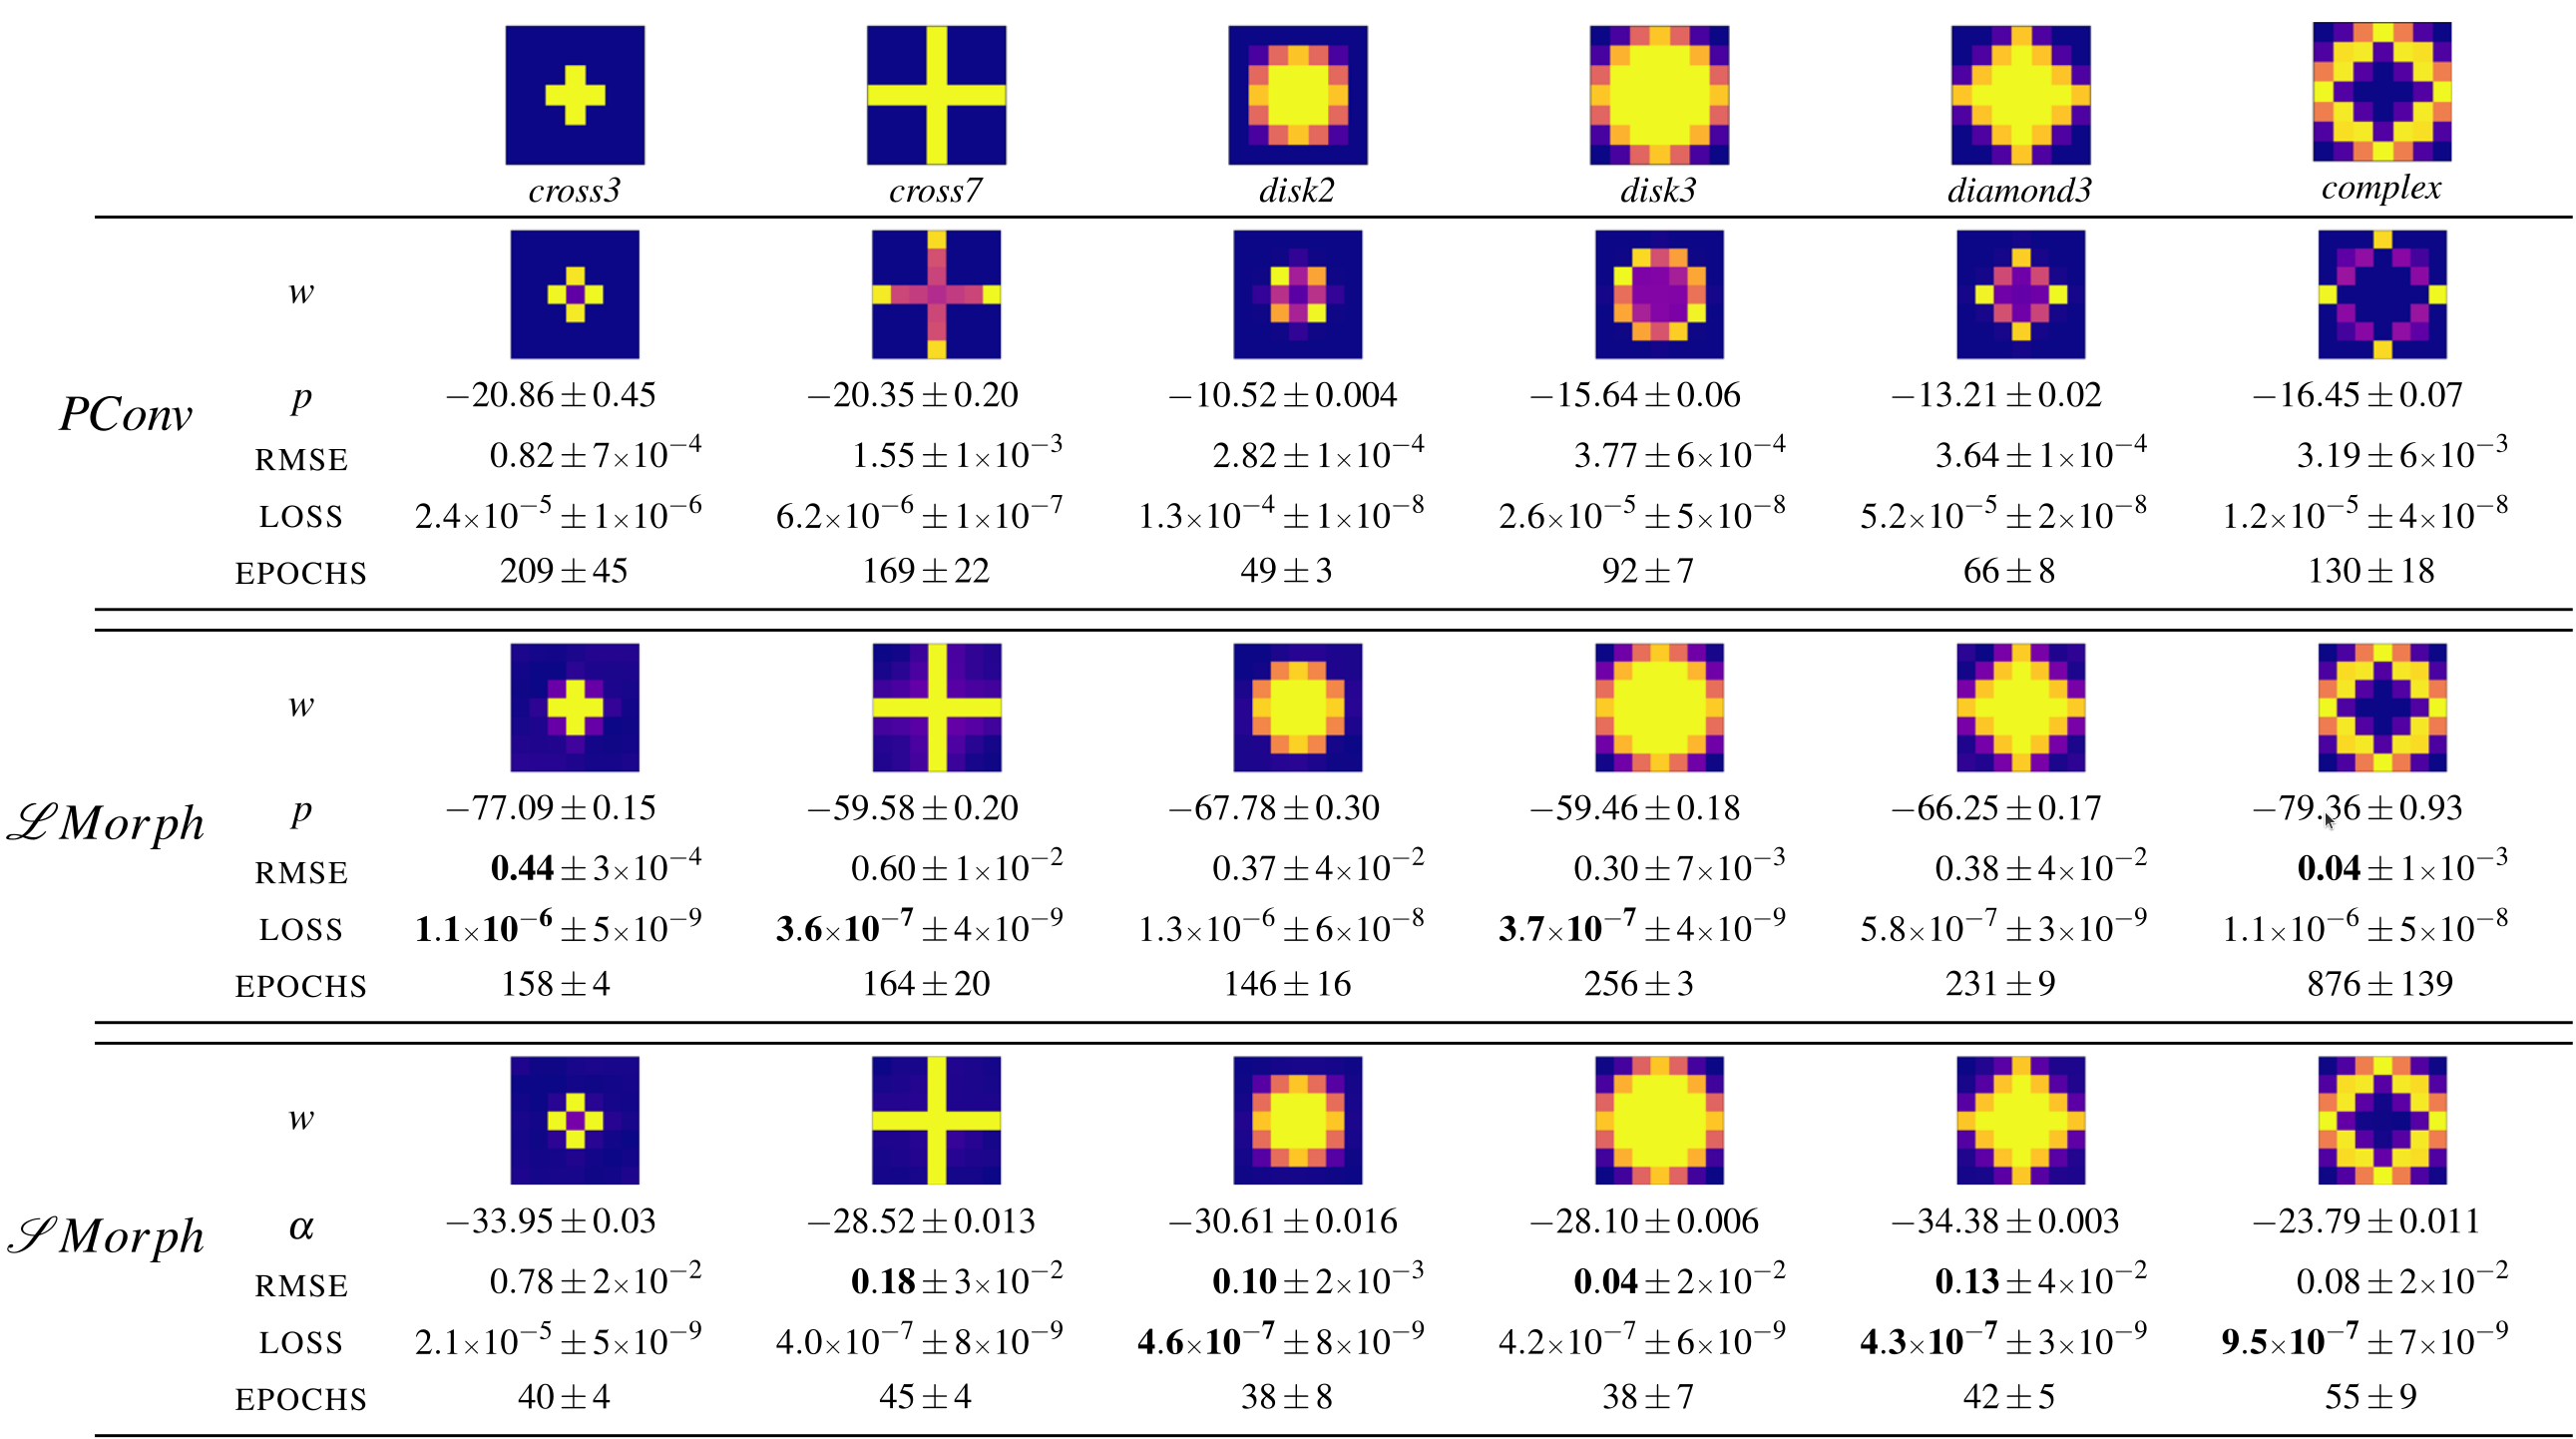
\includegraphics[width=1.00\textwidth]{parts/2-etat_de_lart/D-efficacite_des_reseaux_existant/figures/art_erosion.png}
    \vspace{-2.0mm}
    \caption{ \centering Poids des couches appris et valeur des moyennes et écarts-types des quatre métriques ($p$/$\alpha$, \textit{RMSE}, \textit{loss}, et nombre d'époques) sur cinq runs, pour les trois types de réseaux et les six fonctions structurantes cibles, et pour l'opération cible d'\textbf{érosion}.}
    \label{fig:art_resultats_erosion}
  \end{center}
\end{figure}


\newpage

Dans le deuxième cas, i.e. pour une opération de dilatation avec 1 couche morphologique, on obtient les résultats suivants, sur 5 runs par expérience, fig \ref{fig:art_resultats_dilation} :

% figure
\vspace{2.0mm}
\begin{figure}[ht]
  \begin{center}
    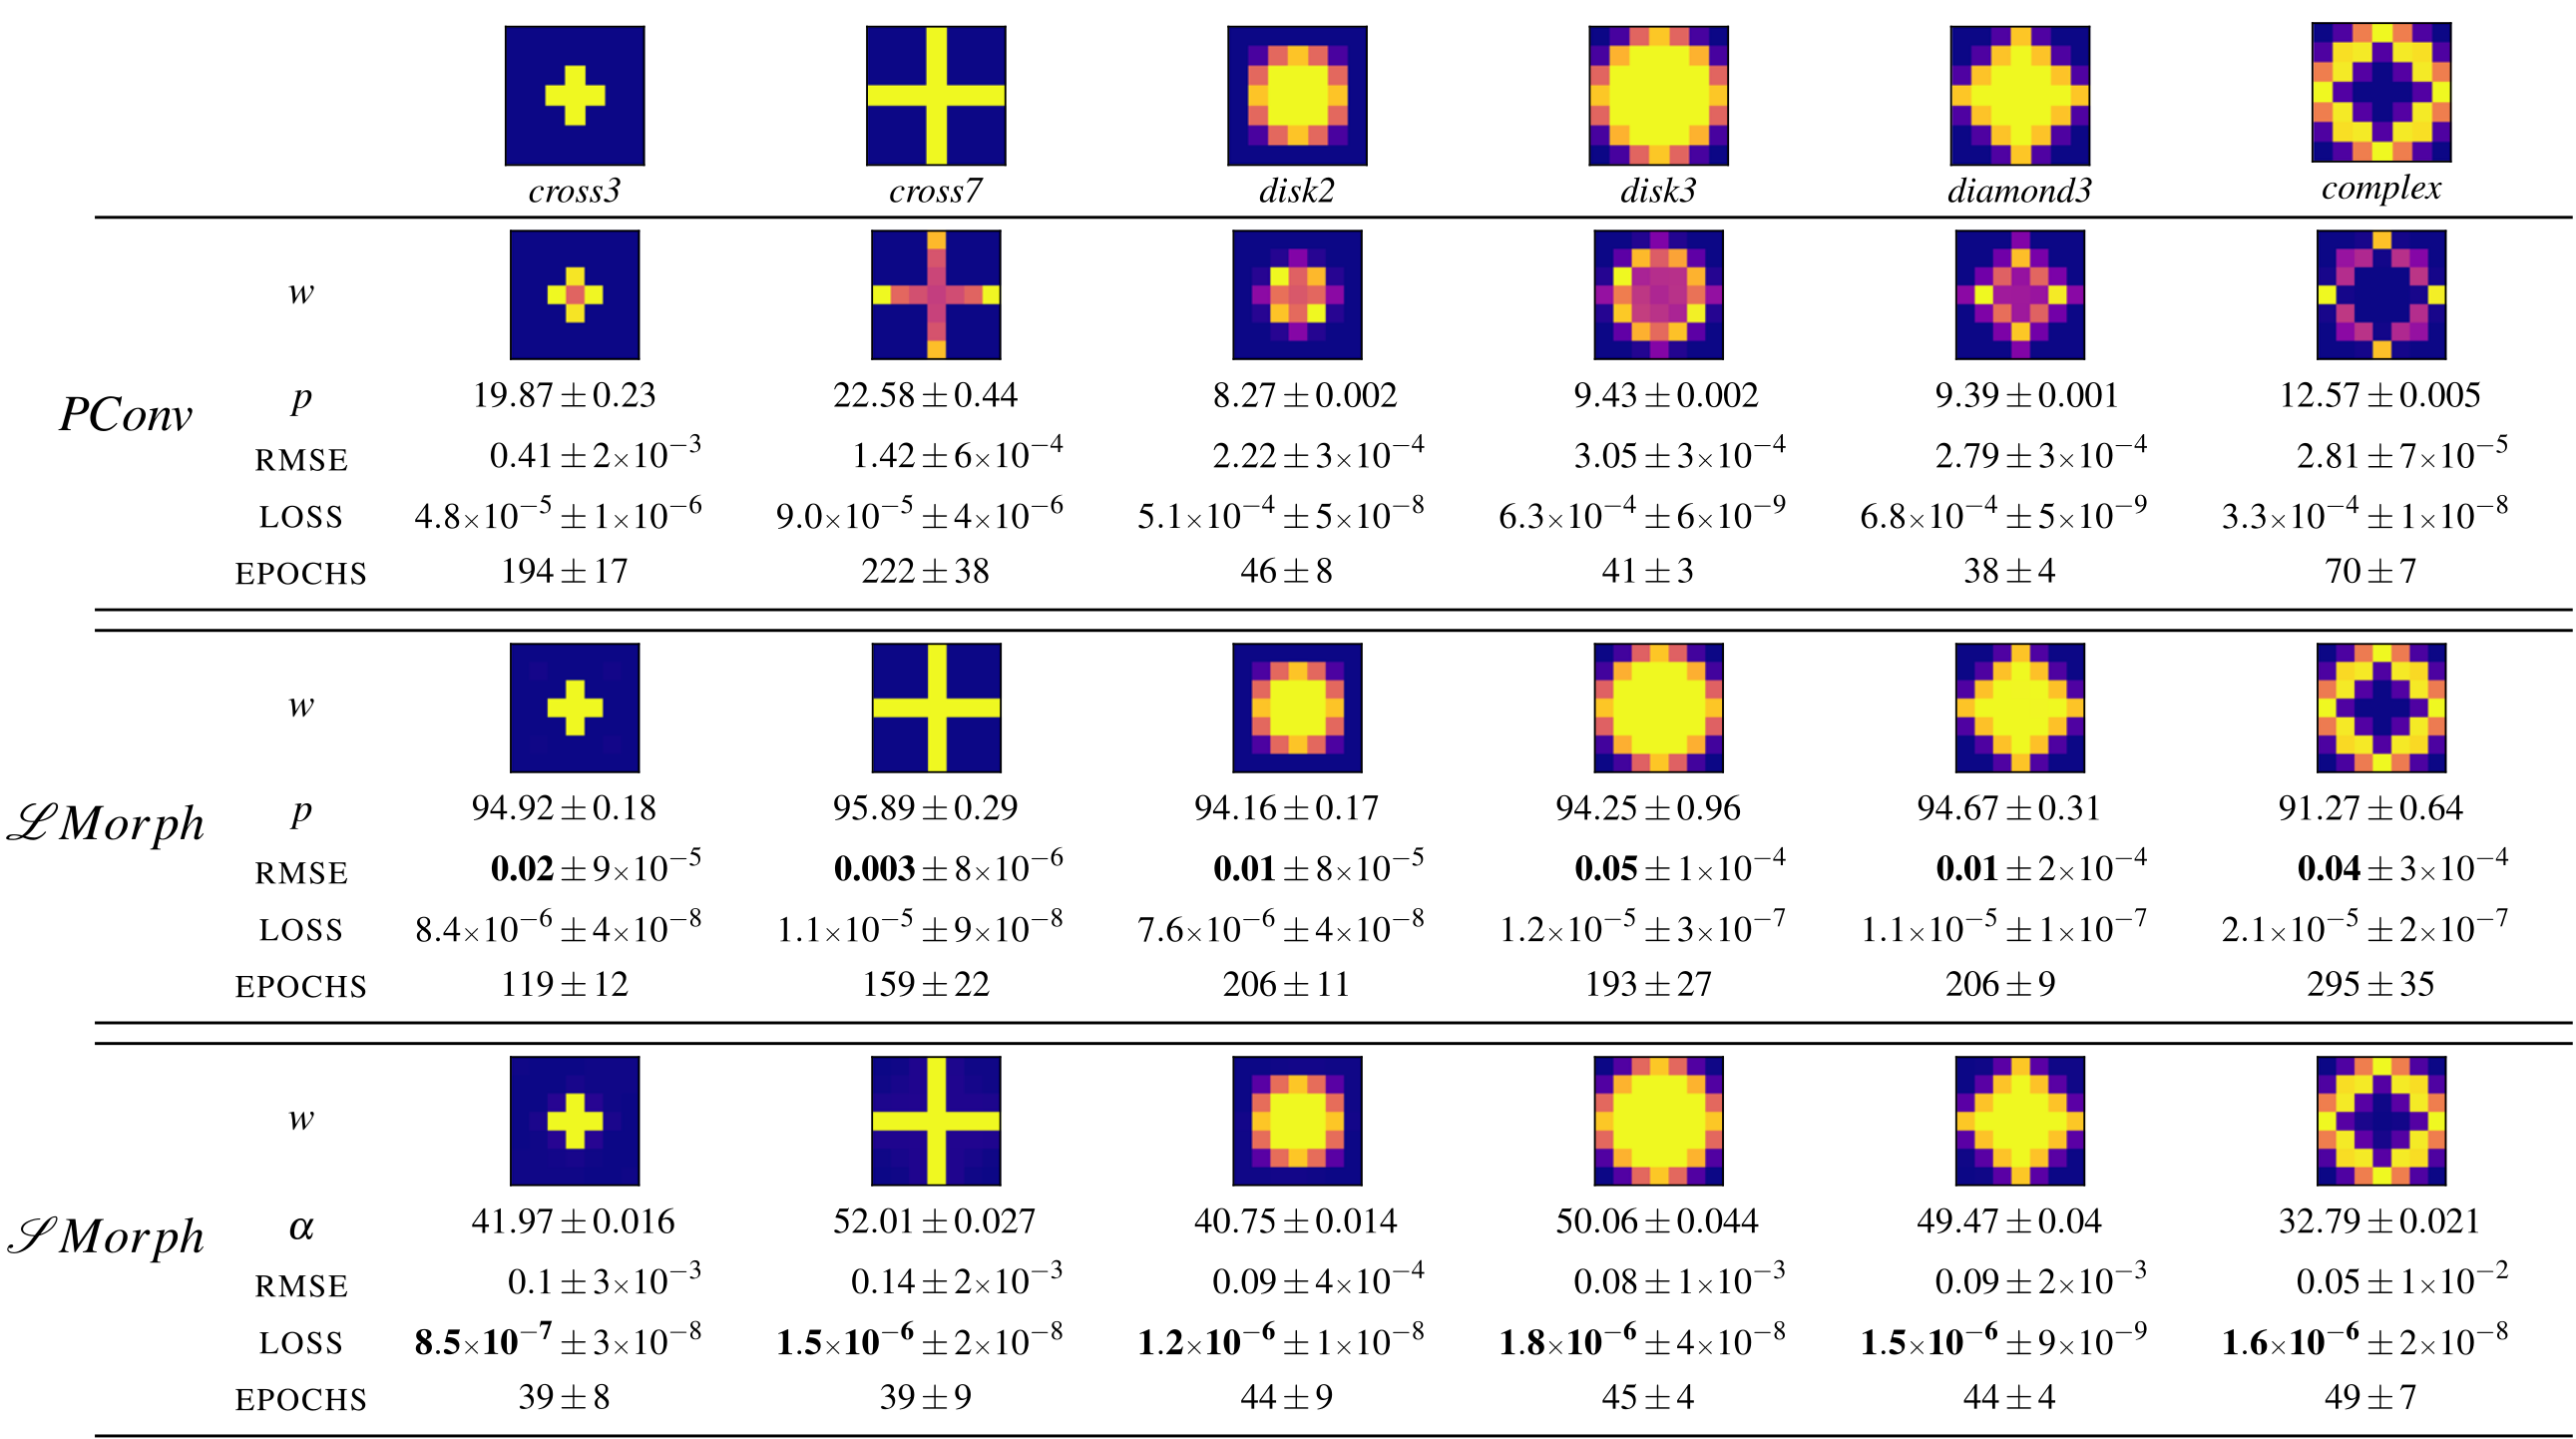
\includegraphics[width=1.00\textwidth]{parts/2-etat_de_lart/D-efficacite_des_reseaux_existant/figures/art_dilation.png}
    \vspace{-2.0mm}
    \caption{ \centering Poids des couches appris et valeur des moyennes et écarts-types des quatre métriques ($p$/$\alpha$, \textit{RMSE}, \textit{loss}, et nombre d'époques) sur cinq runs, pour les trois types de réseaux et les six fonctions structurantes cibles, et pour l'opération cible de \textbf{dilatation}.}
    \label{fig:art_resultats_dilation}
  \end{center}
\end{figure}

\vspace{1.0mm}
A partir des deux figures (fig. \ref{fig:art_resultats_erosion} pour l'ensemble des expériences avec l'érosion, et fig. \ref{fig:art_resultats_dilation} pour celui avec la dilatation), nous pouvons faire les constatations suivantes : \\

%paramètres de contrôle
\noindent D'abord, en examinant la valeur des $p$/$\alpha$ de l'état final des réseaux sur la fig. \ref{fig:art_resultats_erosion} (resp. fig. \ref{fig:art_resultats_dilation}), on constate que les trois types de couches morphologiques parviennent à trouver l'opération morphologique cible, i.e. une érosion (resp. une dilatation), car ces paramètres sont tous négatifs (resp. positifs) et leur amplitude est suffisamment élevée pour considérer l'effet des couches comme véritable opération morphologique. \\

%\vspace{-1.0mm}
\noindent Ensuite, à la fois pour l'érosion et la dilatation, on peut constater que la valeur des RMSE pour l'ensemble des fonctions structurantes cibles est bien plus élevée pour la couche $p$Conv que pour les couches $\mathcal{L}$Morph et $\mathcal{S}$Morph, à l'exception de \textit{cross3}. La forme du noyau des couches $p$Conv est donc moins proche de la cible que les deux autres couches, ce qui peut également être constaté visuellement. La couche $p$Conv semble souffrir d'un certain effet de << creux >> dans la forme de son noyau.


\newpage

\noindent La même chose peut être constatée avec la \textit{loss} des réseaux dans leur état final : elle est bien plus élevée pour la couche $p$Conv, de l'ordre de $10^1$ à $10^2$ fois plus, que pour les couches $\mathcal{L}$Morph et $\mathcal{S}$Morph, qui ont toutes deux le même ordre de grandeur. Ces deux dernières couches sont donc, à la fois pour l'érosion et la dilatation, bien meilleures que la $p$Conv, car elles font de bien meilleures prédictions en moyenne d'après les valeurs de la \textit{loss}. Dans le cadre de la dilatation, fig. \ref{fig:art_resultats_dilation}, la $\mathcal{S}$Morph semble cependant meilleure que la $\mathcal{L}$Morph, d'un ordre de grandeur sur la \textit{loss} en moyenne. \\

\vspace{-1.6mm}
\noindent Le nombre d'époques nécessaire pour atteindre la convergence des réseaux est, pour érosion et dilatation, bien plus faible et régulier sur l'ensemble des expériences pour $\mathcal{S}$Morph que pour $p$Conv ou $\mathcal{L}$Morph. La couche $\mathcal{S}$Morph converge donc plus rapidement et avec plus de régularité que les deux autres couches. 
On remarque également que l'écart-type des métriques sont très faibles, montrant que les réseaux ont convergé sur les 5 cycles d'entraînement (runs) vers la même solution pour les trois couches. \\

%\vspace{-1.0mm}
%Finalement, on peut remarquer que les écarts-types, sur l'ensemble des métriques et des expériences, sont toutes relativement faibles, ce qui indique que les cinq runs (cycles d'entraînement) ont convergé vers la même solution pour les trois couches et les six fonctions structurantes cibles.


\vspace{-1.0mm}
Dans le troisième cas, pour une opération d'ouverture avec 2 couches fig. \ref{fig:art_resultats_opening} : \\
%Dans le troisième cas, i.e. pour une opération d'érosion avec un réseau à 1 couche morphologique, on obtient les résultats de convergence et de caractéristiques suivants, sur 5 runs par expérience, fig \ref{fig:art_resultats_opening} :

% figure
\vspace{-4mm}
\begin{figure}[ht]
  \begin{center}
    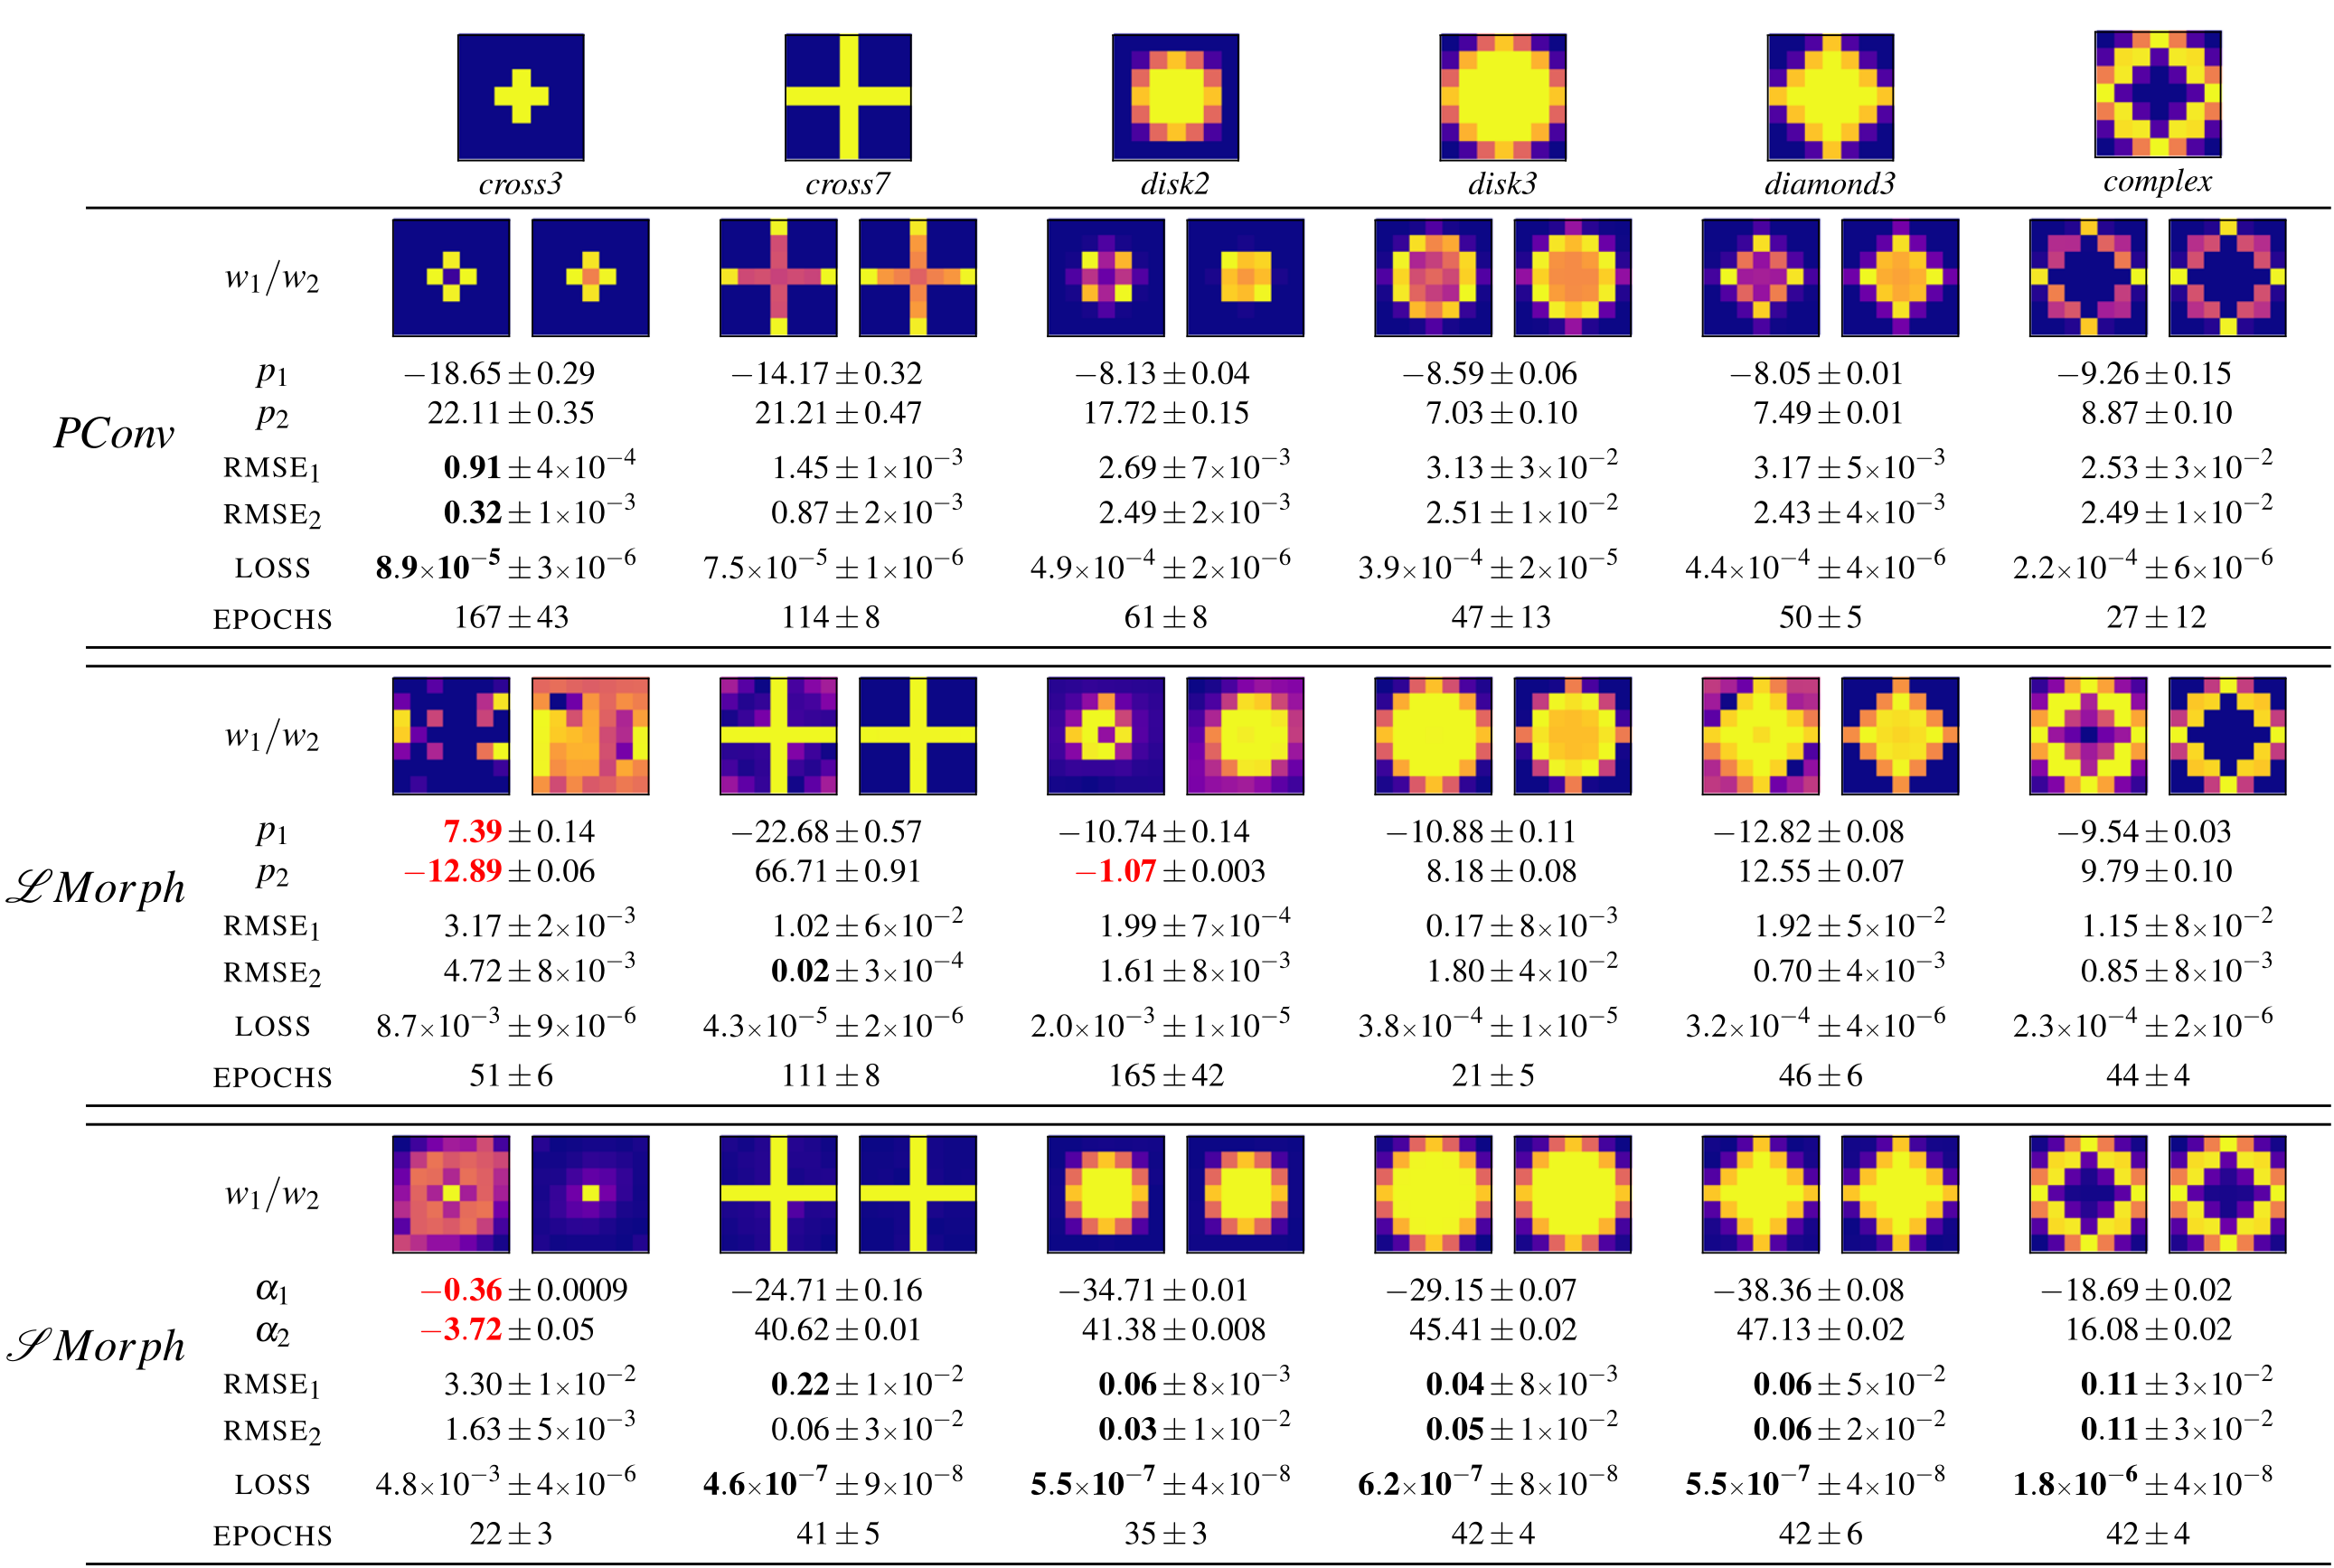
\includegraphics[width=1.00\textwidth]{parts/2-etat_de_lart/D-efficacite_des_reseaux_existant/figures/art_opening.png}
    \vspace{-4.0mm}
    \caption{ \centering Poids des couches appris et valeur des moyennes et écarts-types des quatre métriques ($p$/$\alpha$, \textit{RMSE}, \textit{loss}, et nombre d'époques) sur cinq runs, pour les trois types de réseaux et les six fonctions structurantes cibles, et pour l'opération cible d'\textbf{ouverture}.}
    \label{fig:art_resultats_opening}
  \end{center}
\end{figure}


\newpage

Dans le dernier cas, pour une opération de fermeture avec 2 couches fig. \ref{fig:art_resultats_closing} : \\

% figure
\vspace{-4mm}
\begin{figure}[ht]
  \begin{center}
    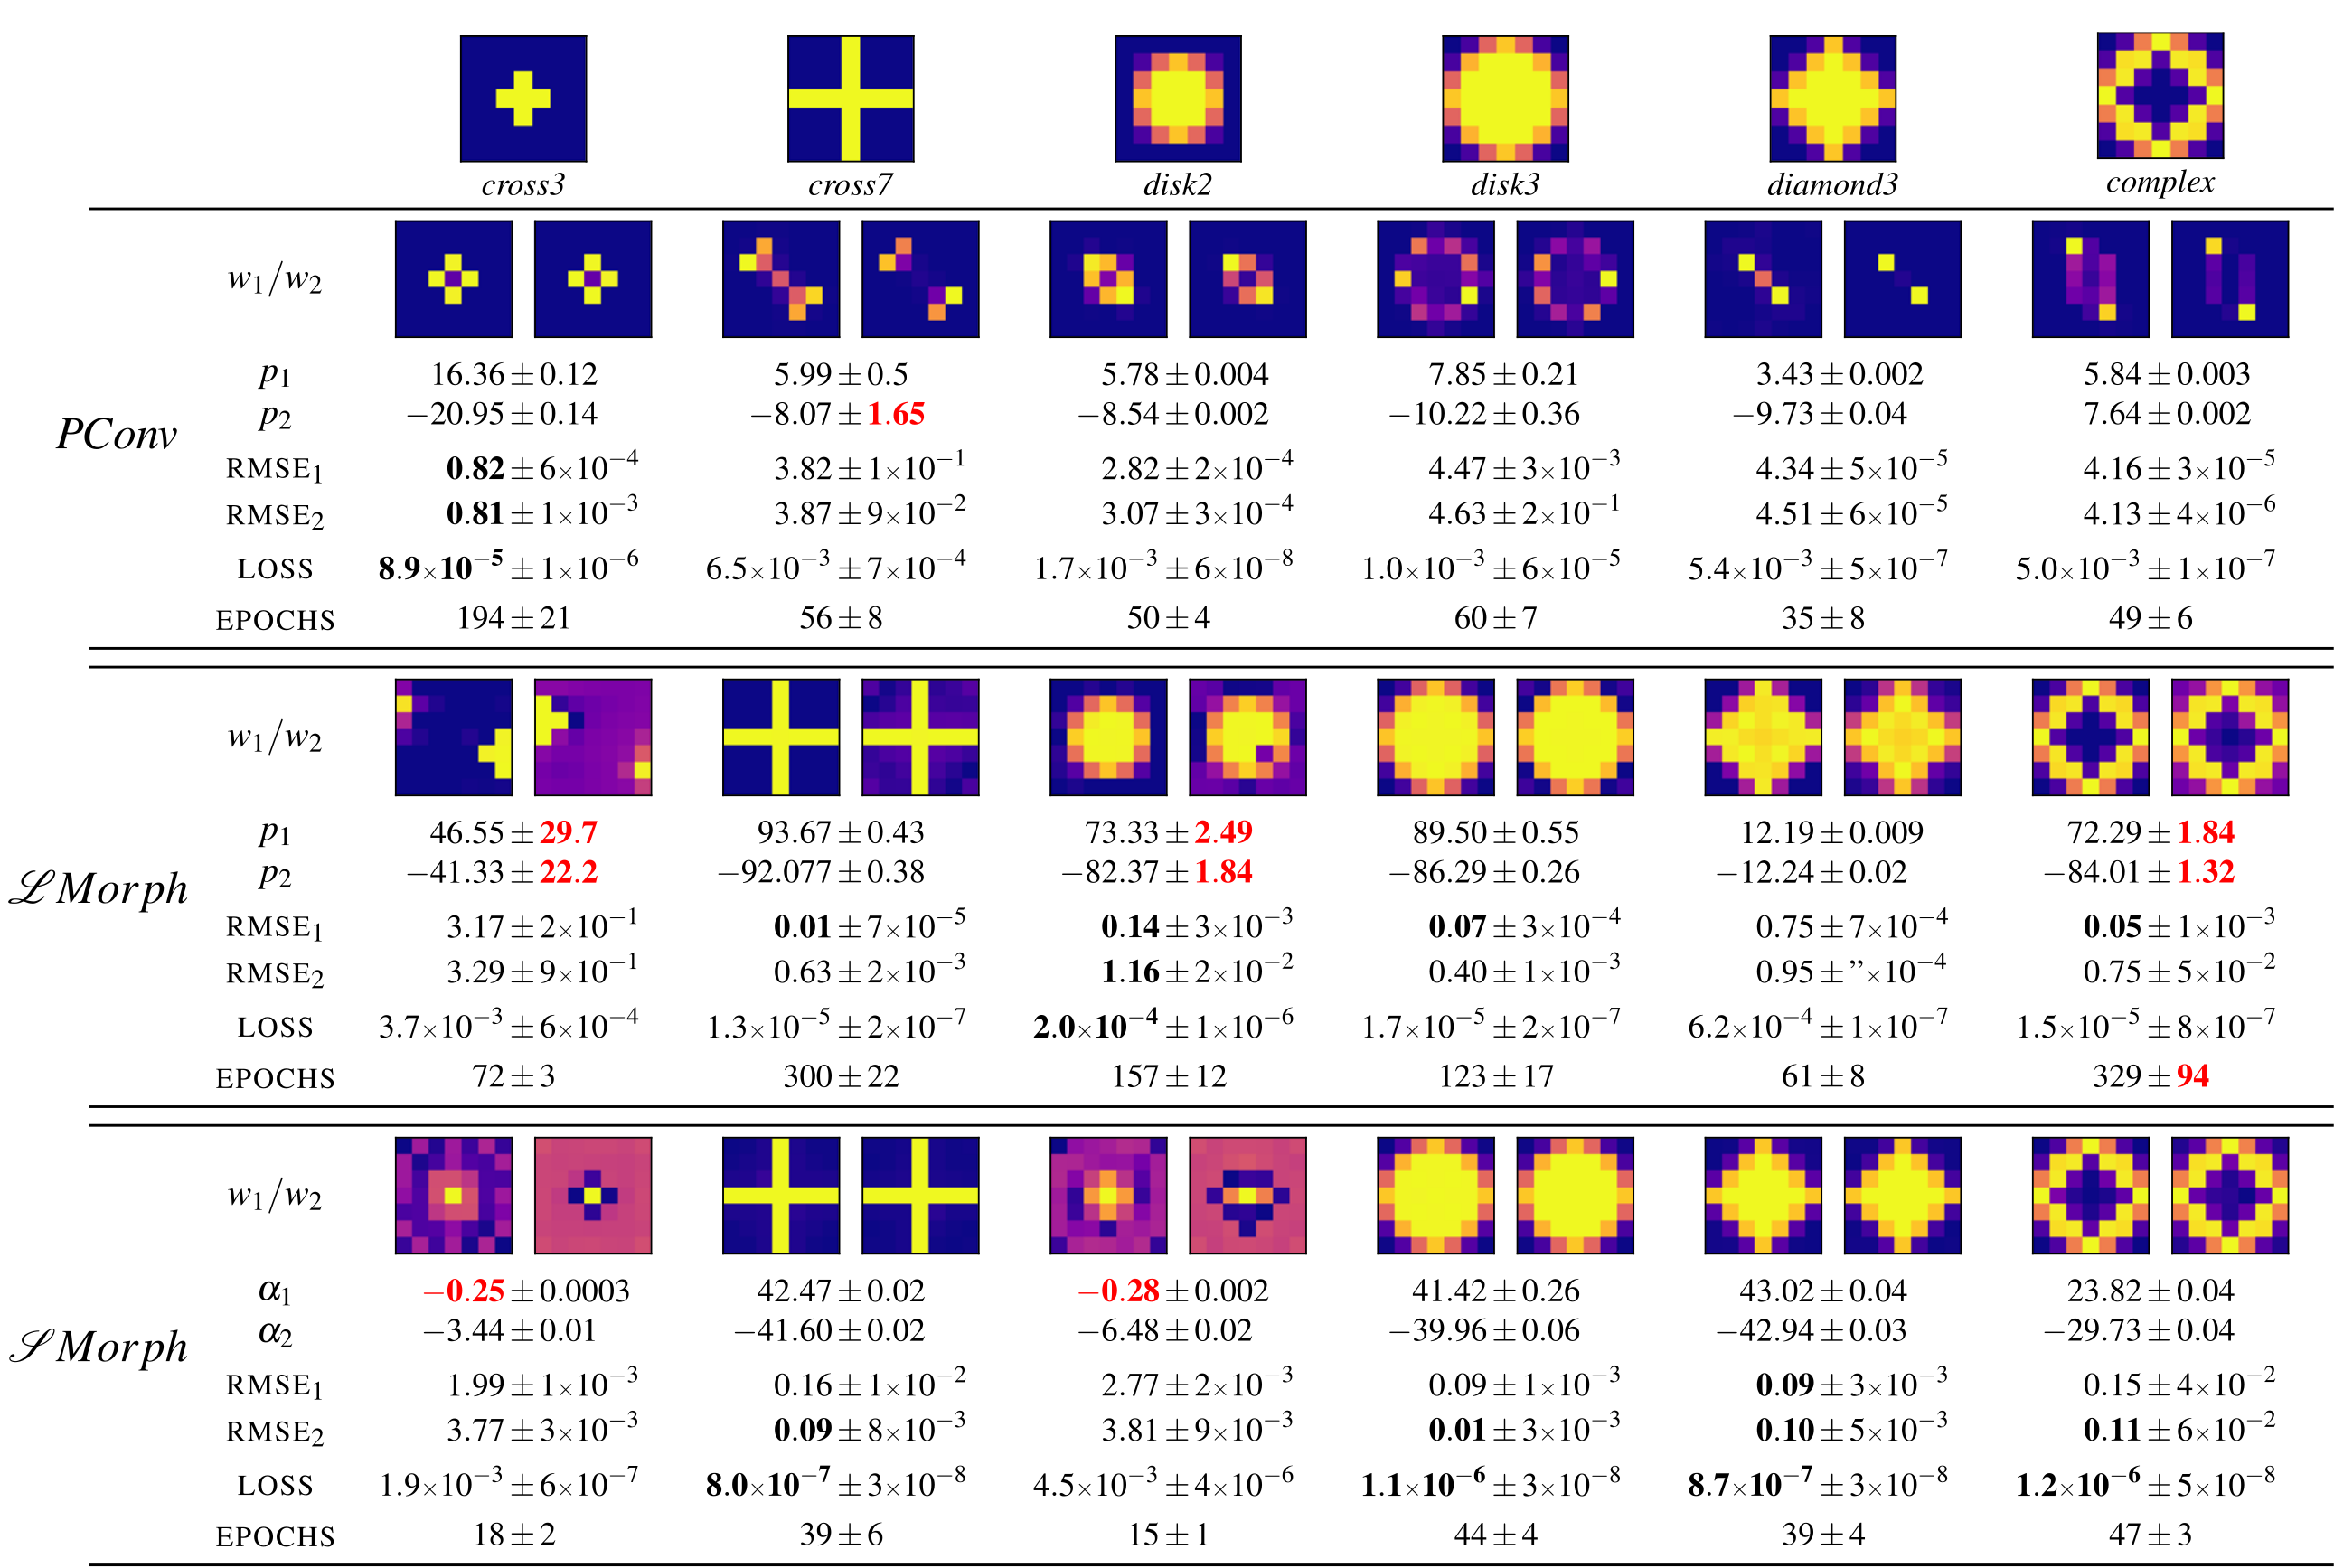
\includegraphics[width=1.00\textwidth]{parts/2-etat_de_lart/D-efficacite_des_reseaux_existant/figures/art_closing.png}
    \vspace{-4.0mm}
    \caption{ \centering Poids des couches appris et valeur des moyennes et écarts-types des quatre métriques ($p$/$\alpha$, \textit{RMSE}, \textit{loss}, et nombre d'époques) sur cinq runs, pour les trois types de réseaux et les six fonctions structurantes cibles, et pour l'opération cible de \textbf{fermeture}.}
    \label{fig:art_resultats_closing}
  \end{center}
\end{figure}


\vspace{-4.2mm}
A partir des deux figures \ref{fig:art_resultats_opening} et  \ref{fig:art_resultats_closing} pour l'ouverture et la fermeture, on remarque la présence évidente d'échecs de convergence. 
Au travers des valeurs de RMSE et des noyaux des couches, on remarque que le réseau $p$ConvNet réussit à plutôt bien deviner la forme de la fonction structurante cible sur l'ensemble des expériences pour l'ouverture, mais pas pour la fermeture où les RMSE et la loss sont tous très élevés. Dans les deux cas, $p$ConvNet souffre toujours de l'effet << creux >>. \\
%Au travers des valeurs des RMSE et de l'aspect visuel du noyau des couches appris, on remarque d'abord que le réseau pConv réussit, pour l'ouverture, plutôt bien à deviner la forme de la fonction structurante cible sur l'ensemble des expériences, mais souffre toujours de l'effet <<creux>>. Pour la fermeture, à l'inverse, les formes apprises sont des échecs, qui s'illustrent à la fois par la haute valeur des RMSE des deux couches pour chaque expérience, et par la valeur bien trop élevée des loss du réseau pConv. \\

\vspace{-1.8mm}
\noindent Hors-mis la cross3, le réseau $\mathcal{L}$MorphNet semble mieux converger que $p$ConvNet sur l'ensemble des expériences, avec des RMSE et des loss bien plus faibles, à la fois pour l'ouverture et la fermeture. Cependant, la forme du noyau des couches n'est pas parfaite, et varie beaucoup entre la première et la seconde couche du réseau, ce qui n'est pas le cas pour le réseau $\mathcal{S}$MorphNet qui, hors-mis avec le disk2 (fermeture), est meilleur encore et ne présente pas cette disymétrie de noyau entre les deux couches du réseau. $\mathcal{S}$MorphNet surpasse presque toujours $p$ConvNet et $\mathcal{L}$MorphNet en termes de RMSE, de loss et de nombre d'époques, pour à la fois l'ouverture et la fermeture.
%\noindent En-dehors de la cross3, le réseau LMorph semble mieux converger que pConv sur l'ensemble des expériences, avec des valeurs de RMSE et de loss bien plus faibles que ce dernier, à la fois pour l'ouverture et la fermeture. Cependant, la forme du noyau des couches est loin d'être parfaite, et varie beaucoup entre la première et la seconde couche du réseau. Le réseau SMorph, quant à lui, semble meilleur encore que LMorph, hors-mis le cas du disk2 pour la fermeture, avec des RMSE et des loss plus faibles encore, et des formes de noyaux plus proches de la cible et plus stables entre la première et la seconde couche. \\

%%% \noindent En se penchant sur les valeurs des paramètres de contrôle $p$/$\alpha$, on remarque que, dans les cas d'échec, les couches des réseaux n'ont pas convergé vers la bonne opération (entre érosion et dilatation), avec des $p$/$\alpha$ de signe opposé à ce qu'ils devraient prendre, et de faible amplitude, comme c'est le cas par exemple avec cross3 (ouverture et fermeture) pour les réseaux LMorph et SMorph, ou encore avec disk2 (fermeture) pour SMorph. Le signe vers lequel tendent les $p$/$\alpha$ des deux couches d'un réseau semblent jouer un rôle conséquent dans l'échec de convergence de ce dernier. \\

%\noindent Enfin, notamment pour la fermeture, les réseaux semblent peu stables en termes de résultats de convergence, comme le montrent les fortes valeurs d'écart type pour les métriques quantitatives rapportées. \\

%\noindent À l'exception des cas d'échec sur cross3 et disk2, on remarque finalement que SMorph surpasse presque systématiquement PConv et LMorph en termes de RMSE pour les deux couches, en terme de loss à la convergence, et terme de nombre d'époques d'entraînement, et ce à la fois pour l'ouverture et la fermeture. \\

\newpage

\subsubsection{Problèmes de convergence des réseaux}
\vspace{0.2cm}
L'analyse des résultats des différentes expériences précédentes montre une bien meilleure convergence et une meilleure précision des réseaux $\mathcal{S}$MorphNet par rapport aux réseaux $\mathcal{L}$MorphNet et $p$ConvNet. Ces meilleures performances de la part de $\mathcal{S}$MorphNet se traduit à la fois par une plus petite valeur de perte globale \textit{loss} de l'état final des réseaux (et donc de meilleures prédictions), par une plus nette ressemblance des noyaux du réseau avec la fonction structurante cible (avec une RMSE bien plus faible), et par un nombre moyen d'époques bien plus bas pour atteindre la convergence (et donc une plus grande vitesse d'apprentissage). Et ce en moyenne, à la fois pour les expériences d'érosion, de dilatation, d'ouverture et de fermeture. Les réseaux $\mathcal{S}$MorphNet sont donc plus performants et précis que les deux autres existant. \\

\vspace{-1.8mm}
Cependant, l'analyse de ces résultats montre également que les différents réseaux morphologiques souffrent de problèmes de convergence sur différents aspects. Pour les expériences avec des réseaux à une seule couche morphologique (érosion fig. \ref{fig:art_resultats_erosion} ou dilatation fig. \ref{fig:art_resultats_dilation}), aucun problème majeur hors-mis ceux évoqués précédemment n'est à déplorer. Par contre, pour les expériences avec des réseaux à deux couches morphologiques (ouverture fig. \ref{fig:art_resultats_opening} ou fermeture fig. \ref{fig:art_resultats_closing}), les résultats obtenus soulèvent plusieurs problèmes en termes de comportement de convergence pour les couches $\mathcal{L}$Morph et $\mathcal{S}$Morph, en particulier pour les fonctions structurantes cibles cross3 et disk2 (fig. \ref{fig:art_resultats_closing}), où les couches n'arrivent pas à trouver la bonne forme de noyau, voire à trouver la bonne opération ciblée (par rapport au signe de $p$/$\alpha$), et entraînent donc une \textit{loss} sur le réseau plus élevée que les autres expériences et autres fonctions structurantes cibles. \\

\vspace{-1.6mm}
Cela a conduit Hermary et al. \cite{Hermary_2022} à effectuer une analyse plus approfondie de la convergence progressive des poids (noyau et paramètre de contrôle) de ces couches au fil des époques pendant la phase d'entraînement. Pour les réseaux à deux couches morphologiques, il en résulte ainsi les deux principales constatations suivantes : \\

\vspace{-3.0mm}
\begin{itemize}%[leftmargin=*]
    \item[$\bullet$] D'abord, la manière dont les poids des noyaux se mettent à jour tout au long du processus d'apprentissage présente plusieurs similitudes : la convergence vers la forme correcte est plus rapide pour la deuxième couche que pour la première (car ses poids sont mis à jour avant ceux de la première couche lors de la rétropropagation), de même que la convergence du paramètre $p$/$\alpha$ vers une plage de valeurs garantissant que l'opération appliquée par la couche est une bonne approximation d'une dilatation ou d'une érosion (et non que pseudo).
%\end{itemize}
    \vspace{1.6mm}
%\begin{itemize}%[leftmargin=*]
    \item[$\bullet$] Ensuite, le schéma de mise à jour des poids semble commencer sur les bords du noyau, pour ensuite se propager vers le centre. Cette dernière observation pourrait être la raison de l'échec de la convergence pour cross3 et disk2, car l'étendue de ces fonctions structurantes est plus petite que leur support spatial, ne fournissant ainsi aucun point d'ancrage sur les bords pour que les poids se propagent vers le centre du noyau. Mais cela ne reste qu'une hypothèse.
\end{itemize}


\newpage

% Pour dire l'impact de p/a sur les échecs et problèmes de convergence !!
Toujours sur les cas d'échec avec les réseaux à deux couches morphologiques (fig. \ref{fig:art_resultats_opening} et fig. \ref{fig:art_resultats_closing}), si l'on se penche sur les valeurs des paramètres de contrôle $p$/$\alpha$, on remarque que, dans les cas d'échec, les couches des réseaux n'ont pas convergé vers la bonne opération (entre érosion et dilatation), avec des $p$/$\alpha$ de signe opposé à ce qu'ils devraient prendre, et de faible amplitude également, comme c'est le cas par exemple avec cross3 (ouverture et fermeture) pour les réseaux $\mathcal{L}$Morph et $\mathcal{S}$Morph, ou encore disk2 (fermeture) pour $\mathcal{S}$Morph. Le signe vers lequel tendent les $p$/$\alpha$ des deux couches d'un réseau ainsi que leur amplitude semblent en forte correlation avec les échecs de convergence. La condition $|\alpha| > 10$ est en pratique suffisante pour reproduire une dilatation ou une érosion avec $\mathcal{S}$Morph, ce qui n'est pas le cas avec les échecs de convergence, où l'on a donc que des pseudo-opérations. \\


\vspace{0.4mm}
En conclusion, l'étude de Hermary at al. \cite{Hermary_2022} montre que l'\textit{étendue} d'une fonction structurante (i.e. l'espace occupé par les éléments de son support distingués du fond) par rapport à la taille de son support spatial semble être liée à la capacité des couches morphologiques à apprendre correctement cette fonction cible pour l'ouverture et la fermeture, mais cela n'explique pas à lui seul l'ensemble des cas d'échec présentés. 

\vspace{3.0mm}
\noindent La convergence des réseaux vers des minima locaux à forte attraction est également une explication plausible, car l'identification d'une fonction structurante basée uniquement sur des images originales et des images transformées est une tâche sous-déterminée, plusieurs solutions peuvant exister. Par exemple, deux fonctions structurantes symétriquement décalées se compensent mutuellement et sont aussi valides en tant que solution que deux fonctions centrées (résultats que l'on cherche à obtenir). 

\vspace{3.0mm}
\noindent Intégrer des informations à priori (symétrie, étendue spatiale) sur la fonction structurante recherchée dans la fonction de perte d'entraînement optimisée pourrait être une solution potentielle, mais ces informations a priori pourraient être difficiles à obtenir dans des cas d'utilisation pratiques, lorsque l'on ne connait pas la forme cherchée.

\vspace{3.0mm}
\noindent Cette étude de Hermary et al. a permis de mieux comprendre l'impact de la rétropropagation du gradient, lors de l'entraînement des réseaux, dans la tendance de la seconde couche à mieux converger vers la solution attendue, ses poids se mettant à jour en premier par rapport à la première couche. Elle montre également que la valeur, en particulier le signe, du paramètre de contrôle $p$/$\alpha$ des couches morphologiques semble fortement correlée à la bonne ou mauvaise convergence des réseaux. \\


\vspace{0.6mm}
Pour la suite, la couche $\mathcal{S}$Morph ayant démontré de bien meilleurs résultats de convergence et de précision par rapport aus deux autres couches $\mathcal{L}$Morph et $p$Conv, nous travaillerons uniquement sur cette couche-ci. L'objectif sera alors d'étudier plus en profondeur le comportement des réseaux $\mathcal{S}$MorphNet, et de trouver des solutions pour améliorer la convergence de ces réseaux afin d'éviter les cas d'échecs tels que ceux présentés dans cette partie. Il s'agira d'un travail principalement exploratoire.

%%%%% NE PAS OUBLIER DE METTRE LES REFERENCES DANS L'ETAT DE L'ART!!!! %%%%%
%\noindent 1. Scanner tout l'état de l'art et ajouter les références là où besoin\\     --- OK
%\noindent 2. Remplacer tous les [ref] ou ref ou [] par les références adéquates\\      --- OK
%\noindent 3. Repasser les références, et vérifier qu'il n'y ait pas de \textit{null}!! --- OK
\newpage

%========================================================================================
%	3. AMELIORATION DES RESEAUX
%========================================================================================

\section{Amélioration des réseaux}

% Réseaux SMorphNet-Tanh
\subsection{Réseau $\mathcal{S}$MorphNet-Tanh} %Réseaux SMorphNet-Tanh

\subsubsection{Contexte et motivations}
\vspace{0.2cm}
Les résultats précédents montrent qu'il reste encore quelques cas d'échecs de convergence pour les réseaux $\mathcal{S}$MorphNetTanh à deux couches morphologiques, avec les opérations cibles d'ouverture et de fermeture, et ce malgré l'ajout d'un partage doux des poids entre les noyaux $w$ des deux couches et l'ajout dans la \textit{loss} d'une contrainte $C_\text{awayOPP}$ entre les deux paramètres de contrôle $\alpha$ (ou $p$) associés. \\

\vspace{-1.4mm}
\noindent La modulation de l'initialisation des noyaux $w$ du réseau devient alors une solution potentielle à ces derniers échecs. ALors que les poids des noyaux sont originellement initialisés selon une loi normale centrée réduite afin de brasser les différents états de convergence possibles à partir d'initialisations aléatoires différentes sur plusieurs expériences, on peut finalement se dire que cette forme initiale des noyaux peut être fixée et définie de manière déterminée au préalable, selon des caractéristiques morphologiques générales à priori que l'on connait ou que l'on recherche sur ces noyaux. \\

\vspace{-1.4mm}
\noindent En l'occurence, on peut facilement s'imaginer que ce que l'on recherche ou favorise dans nos différents cas d'étude, c'est une forme de noyaux centrée sur son support et peu dispersée. On choisira alors une initialisation sous la forme d'une gaussienne 2D, allant de $0$ aux coins de l'image des noyaux à $1$ en son centre (voir figure \ref{fig:init_gauss} suivante). \\


%figure
\vspace{-1.0mm}
\begin{figure}[htp]
  \begin{center}
    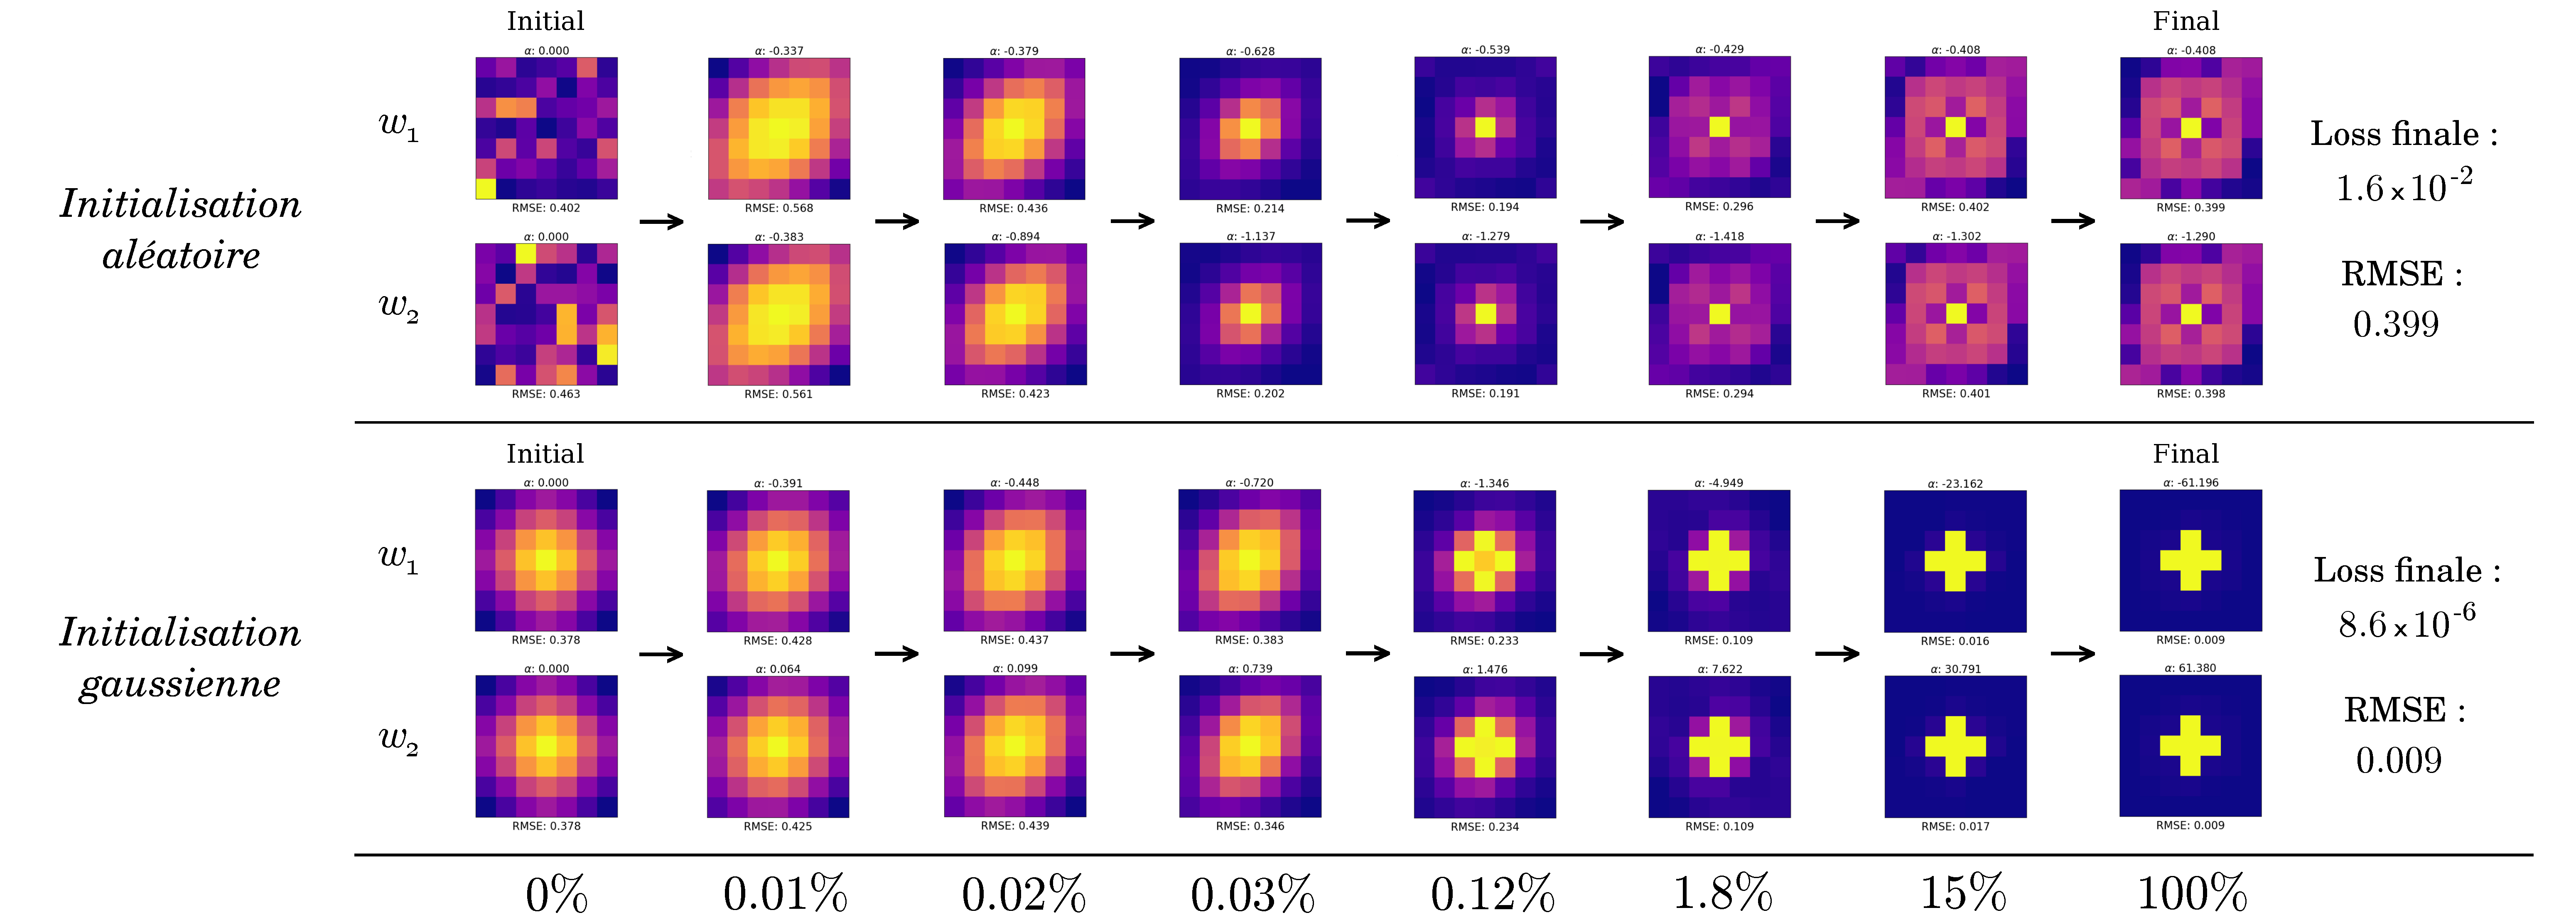
\includegraphics[width=1.00\linewidth]{parts/3-contributions/D-modulation_de_l_initialisation/figures/k_gauss.pdf}
    \vspace{-4.0mm}
    \caption{ \centering Évolution de la forme du noyau des deux couches du réseau et de sa \textit{RMSE} en fonction de la progression de l'entraînement (en \% avant l'état final), pour le \textit{cross3} et l'ouverture sur la banque MNIST, avec initialisation aléatoire et init. gaussienne.}
    \label{fig:init_gauss}
  \end{center}
\end{figure}


\vspace{-3.0mm}
\noindent L'exemple fig. \ref{fig:init_gauss}, obtenu sur six runs, montre bien ici l'efficacité de cette initialisation gaussienne des noyaux $w$ par rapport à l'aléatoire normale centrée réduite sur \textit{cross3} pour l'ouverture sur MNIST, avec des valeurs de \textit{RMSE} et de \textit{loss} bien plus faibles.

\newpage

\subsubsection{Formalisation}
\vspace{0.2cm}
L'idée dans la formule de cette nouvelle couche $\mathcal{S}$MorphTanh dérivée de $\mathcal{S}$Morph est simplement d'ajouter un facteur multiplicateur devant les valeurs du noyau $w$ dans la formule de $\mathcal{S}$Morph (\ref{SMorph}), facteur qui puisse être le reflet d'une transition lisse entre le signe $+$ et $-$ lors du passage de $\alpha$ d'un signe positive à un signe négatif, et inversement. Ce facteur est ici défini par la tangente hyperbolique de $\alpha$ : $\tanh{(\alpha)}$. \\

La formule de $\mathcal{S}$MorphNetTanh, pour une image $f: I \subseteq \mathbb{Z}^2 \rightarrow \mathbb{R}$ et un noyau de couche $w: W \subseteq \mathbb{Z}^2 \rightarrow \mathbb{R}$, et avec $\alpha \in \mathbb{R}$, est ainsi définie pour tout $x \in I$ par :

\begin{equation}
    \pmb{\mathcal{S}}\textbf{MorphTanh} (f,w,\alpha)(x) = \frac{\sum_{y \in \breve{W}_x} (f(y) + \tanh{(\alpha)} w(x-y))e^{\alpha (f(y) + \tanh{(\alpha)} w(x-y))}}{\sum_{y \in \breve{W}_x} e^{\alpha (f(y) + \tanh{(\alpha)} w(x-y))}}
    \label{SMorphTanh}
\end{equation}

\vspace{3.0mm}
\noindent Le facteur $\tanh{(\alpha)}$ permet bien, à la fois, d'ajuster le signe de $w$ dans la formulation asymptotique de $\mathcal{S}$Morph, et de lisser l'espace de la \textit{loss} pour $\alpha$ au voisinage de $0$, en réduisant l'impact des variations des poids $\text{w}_i$ dans la formule de $\mathcal{S}$MorphTanh, grâce à ce $\tanh{(\alpha)}$ devant $w$, qui est proche de $0$ quand $\alpha$ est au voisinage de $0$. \\

%figure
\vspace{-1.5mm}
\begin{figure}[ht]
  \begin{center}
      \subfigure[$(\text{w},\alpha) \mapsto \text{w}$]{
          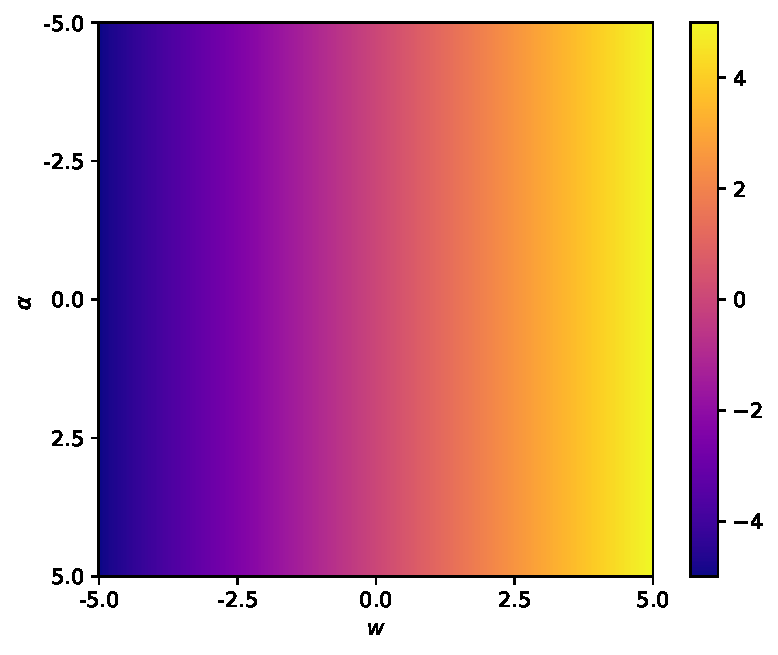
\includegraphics[width=0.30\textwidth]{parts/3-contributions/A-reseaux_smorphTANH/figures/image_wa_s.pdf}
          \label{fig:suh1}}
      \hspace{12.0mm}
      \subfigure[$(\text{w},\alpha) \mapsto \tanh{(\alpha)} \times \text{w}$]{
          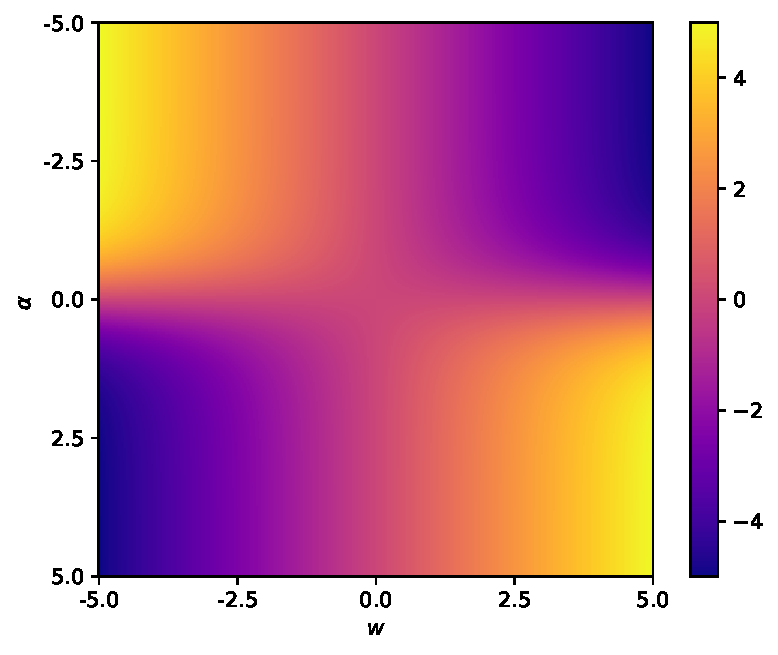
\includegraphics[width=0.30\linewidth]{parts/3-contributions/A-reseaux_smorphTANH/figures/image_wa_sh.pdf}
          \label{fig:suh2}}
    \caption{ \centering Carte de la fonction $(\text{w},\alpha) \mapsto \text{w}$ représentant $\mathcal{S}$MorphNet (gauche \ref{fig:suh1}) et de la fonction $(\text{w},\alpha) \mapsto \tanh{(\alpha)} \times \text{w}$ représentant $\mathcal{S}$MorphNetTanh (droite \ref{fig:suh2}).}
    \label{fig:espace_s_vs_sh}
  \end{center}
\end{figure}

\vspace{-4.0mm}
\noindent La figure \ref{fig:espace_s_vs_sh} ci-dessus montre l'évolution des valeurs (en couleurs) de la fonction $(\text{w},\alpha) \mapsto \tanh{(\alpha)} \times \text{w}$ en fonction de w (en abscisse) et $\alpha$(en ordonnée). La carte \ref{fig:suh1} reflète le comportement de $\mathcal{S}$Morph sur une image $f$ nulle et avec un seul poids w du noyau $w$, et la carte \ref{fig:suh2} reflète celui de $\mathcal{S}$MorphTanh. On remarque bien sur \ref{fig:suh1} le passage continue d'un signe positif à un signe négatif de $\alpha$ en ordonnée, ainsi que le lissage de la fonction au voisinage de $\alpha \approx 0$ selon le poids w en abscisse. \\
%\noindent La figure ci-dessus montre l'évolution des valeurs de la fonction $(\text{w},\alpha) \mapsto \tanh{(\alpha)} \times \text{w}$ avec le passage continue d'un signe positif à un signe négatif de $\alpha$ en ordonnée. Il montre également le lissage, au voisinage de $\alpha \approx 0$, de la fonction $\textit{w} \mapsto \tanh{(\alpha)} \times \text{w}$ selon le poids \textit{w} sur l'axe des abscisses. \\

\vspace{-1.6mm}
\noindent On obtient bien l'image $f \ominus \breve{w}$ quand $\alpha \rightarrow -\infty$, et toujours $f \oplus w$ quand $\alpha \rightarrow +\infty$.

\newpage

\subsubsection{Comparaison avec $\mathcal{S}$MorphNet}
\vspace{0.2cm}
Pour savoir si les réseaux $\mathcal{S}$MorphNetTanh sont des réseaux d'intérêt, au-delà de l'amélioration de la formulation asymptotique des couches $\mathcal{S}$MorphTanh quand $\alpha \rightarrow -\infty$ par rapport à celle des couches $\mathcal{S}$Morph telle que vue précédemment, il faut étudier les performances de ces nouveaux réseaux sur un ensemble d'expériences et comparer leurs résultats à ceux des réseaux $\mathcal{S}$MorphNet simples. \\

\vspace{-1.6mm}
%Pour comparer avec rigueur la précision et l'efficacité des deux réseaux $\mathcal{S}$MorphNet et $\mathcal{S}$MorphNetTanh, ...
\noindent Dans cet objectif, on reprend le même protocole d'expérimentation que dans l'état de l'art, où l'on étudie l'état des réseaux après leur entraînement avec certaines métriques. En particulier : 

\vspace{0.4mm}
\begin{itemize}%[leftmargin=*]
    \item[$\bullet$] on reprend les quatre mêmes métriques d'évaluation de la performance des réseaux que dans l'état de l'art (partie 2.4) ;
    \item[$\bullet$] on reste sur la banque d'images en niveaux de gris MNIST ;
    \item[$\bullet$] on fait cette fois-ci six runs par expérience, au lieu de cinq ;
    \item[$\bullet$] on considère cette fois huit fonctions structurantes, en prenant les six précédentes de l'état de l'art, et en y ajoutant une fonction structurante diagonale asymétrique \textit{adiag} et une autre plate aléatoire \textit{brand}.
\end{itemize}

\vspace{2.2mm}
On résume, comme dans l'état de l'art, les résultats de l'ensemble des expériences en quatre groupes : le premier pour les expériences avec l'érosion pour opération cible (réseaux à une couche morphologique), le deuxième avec la dilatation (1 couche), le troisième avec l'ouverture (2 couches), et le dernier avec la fermeture (2 couches). \\

%\vspace{-0.6mm}
Pour l'érosion sur des réseaux à une couche, on obtient les résultats suivants :

% figure
\vspace{4.0mm}
\begin{figure}[ht]
  \begin{center}
    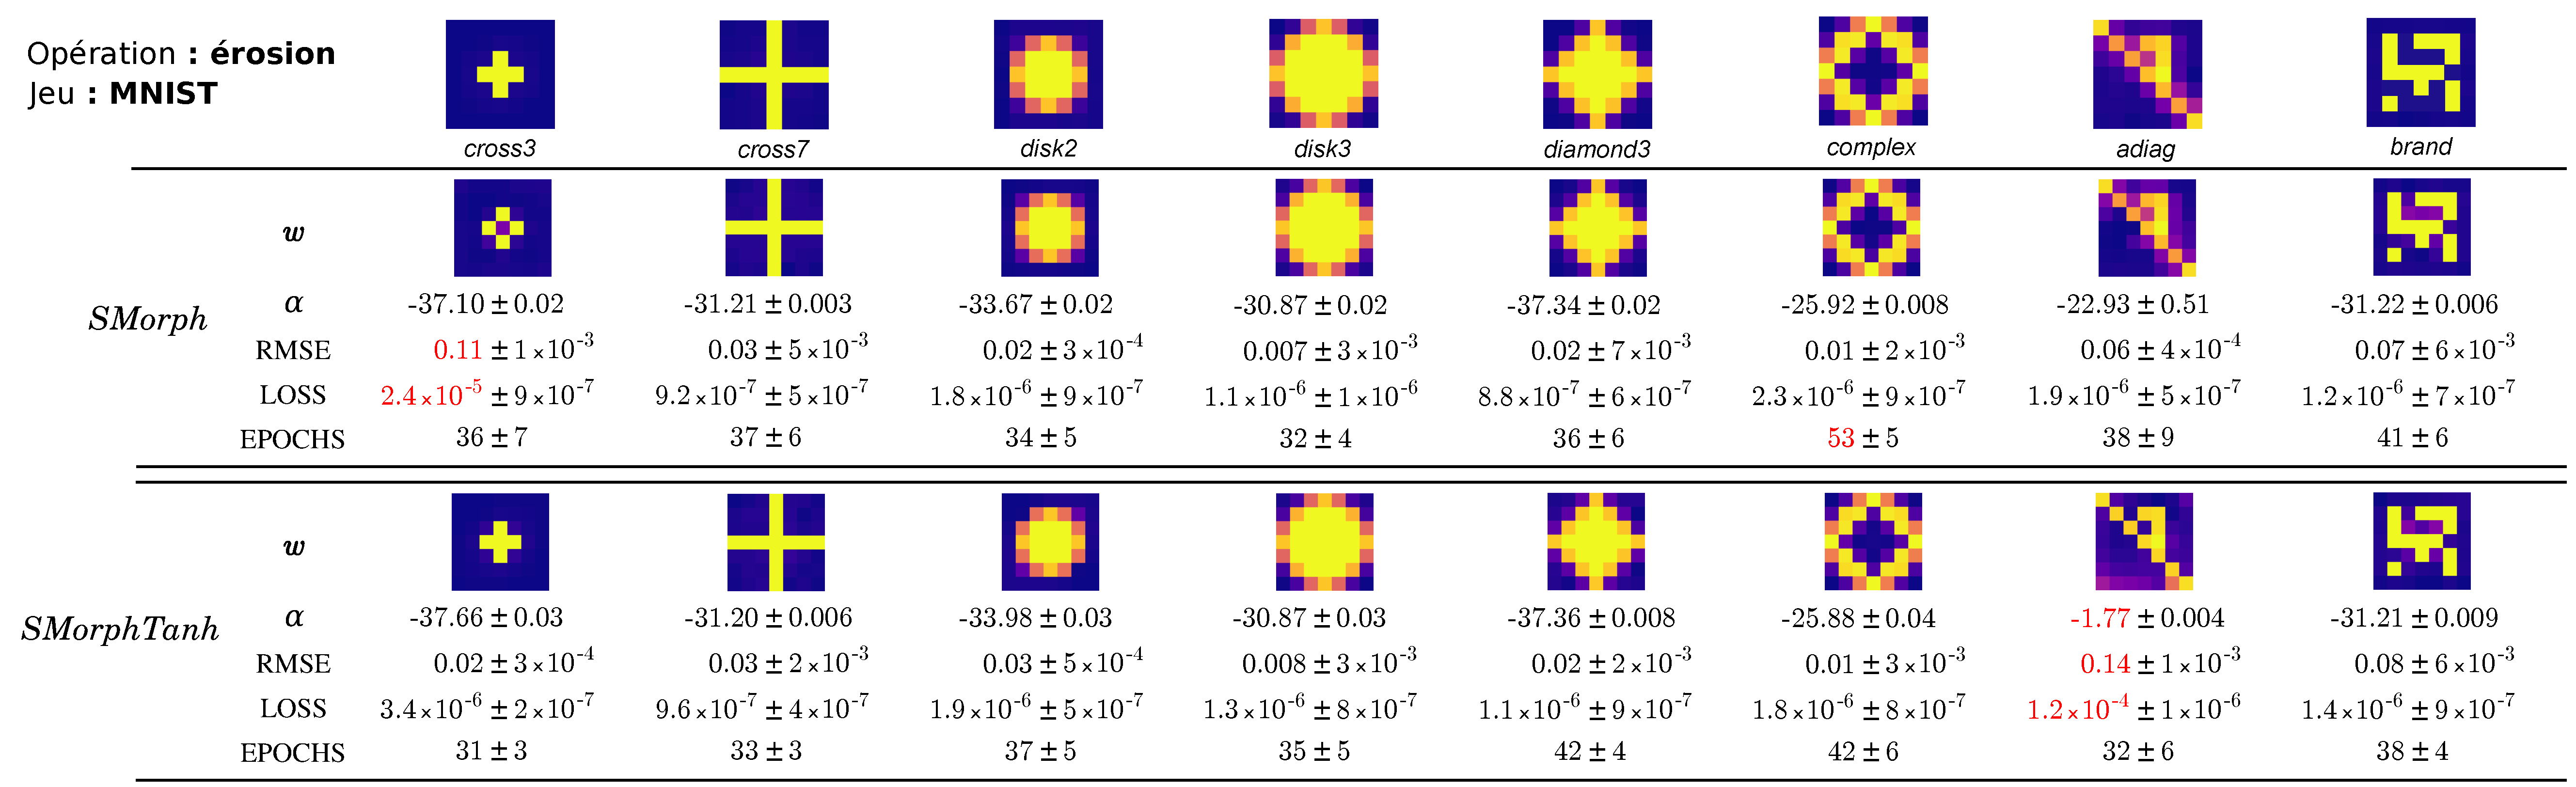
\includegraphics[width=1.00\textwidth]{parts/3-contributions/A-reseaux_smorphTANH/figures/t_erosion_mnist.pdf}
    \vspace{-2.0mm}
    \caption{ \centering Comparaison des poids appris et des moyennes et écarts-types des métriques $\alpha$, \textit{RMSE}, \textit{loss} et nombre d'époques, et ce sur six runs, entre $\mathcal{S}$Morph et $\mathcal{S}$MorphTanh à une couche, pour les huit fonctions structurantes cibles et l'opération d'\textbf{érosion}.}
    \label{fig:SMvsSMTH_erosion_mnist}
  \end{center}
\end{figure}


\newpage

\noindent En rouge sont notées les moins bonnes performances moyennes du réseau par rapport à l'autre (grandes moyennes). En vert, les résultats instables (grands écarts-types). \\

\vspace{2mm}
%Pour l'opération cible de dilatation sur des réseaux à une seule couche morphologique, on obtient les résultats suivants : \\
Pour la dilatation sur des réseaux à une couche, on obtient les résultats suivants : \\

% figure
\vspace{2.5mm}
\begin{figure}[ht]
  \begin{center}
    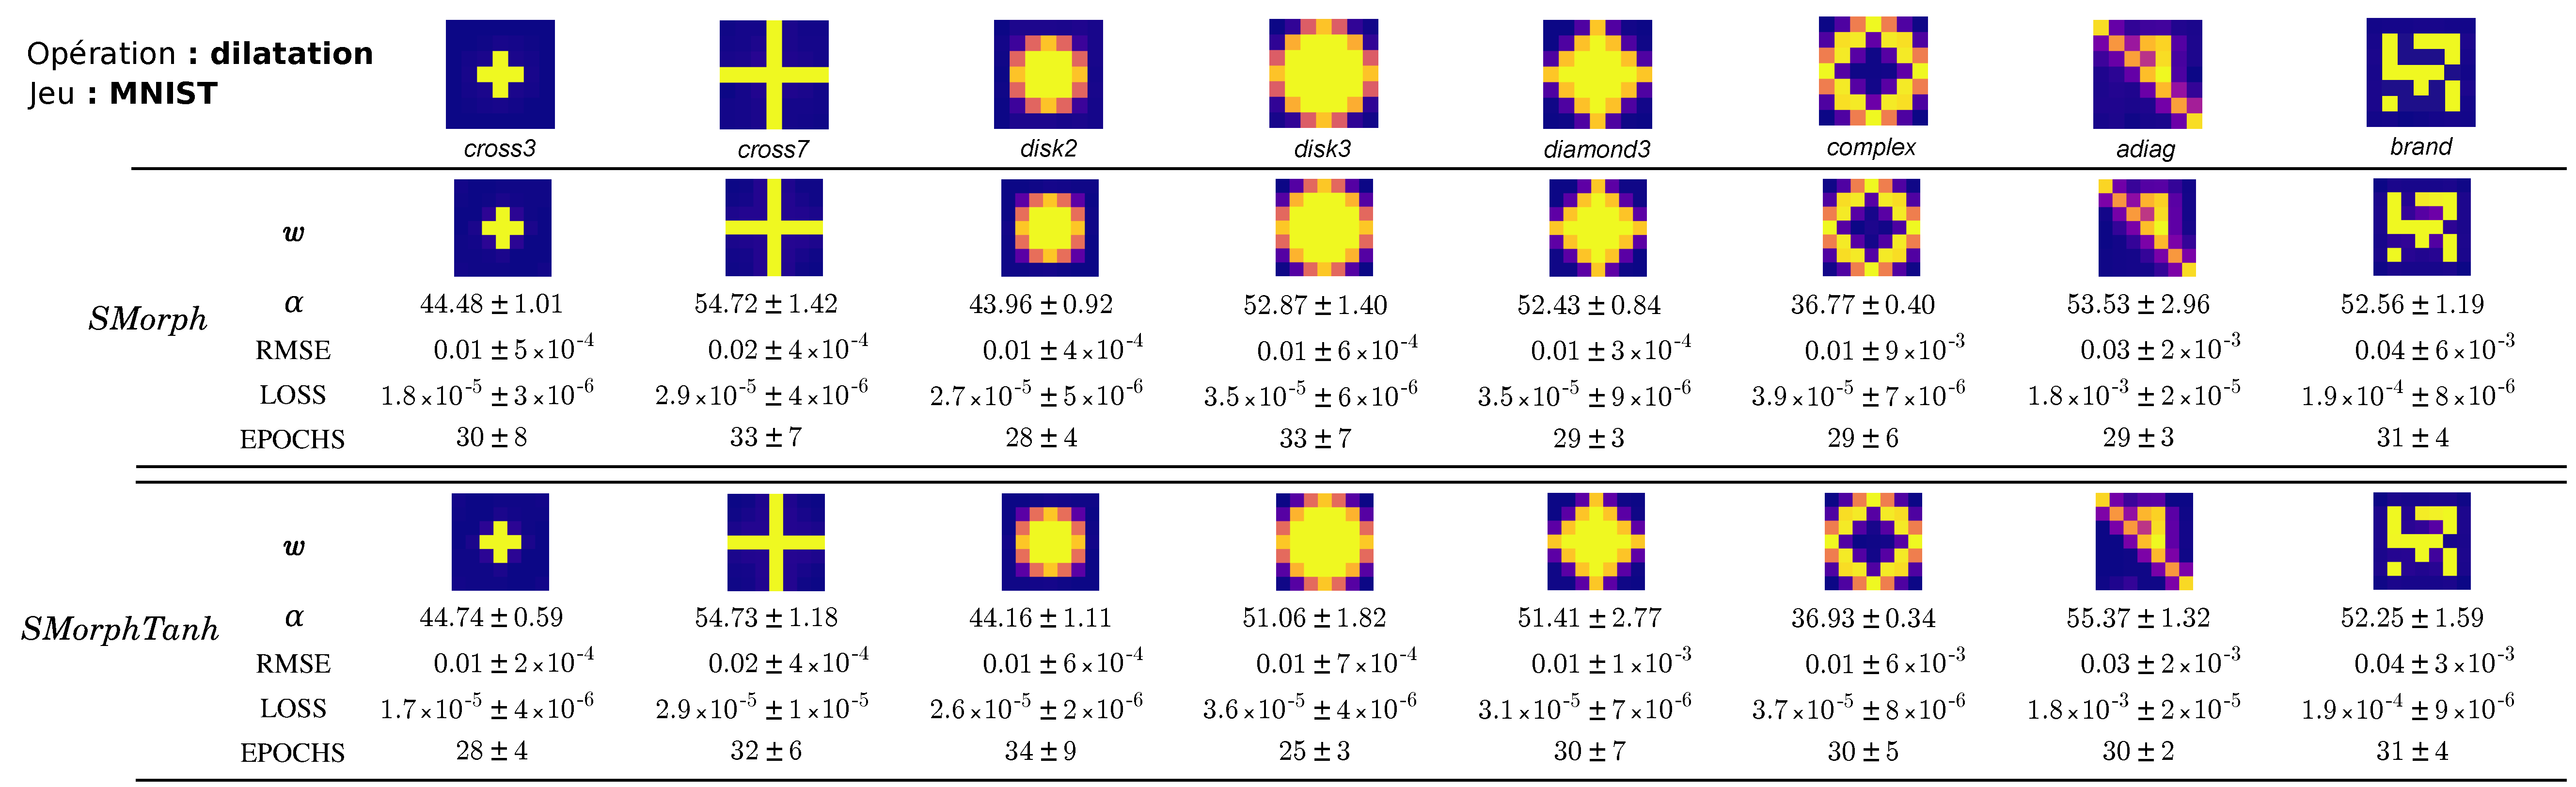
\includegraphics[width=1.00\textwidth]{parts/3-contributions/A-reseaux_smorphTANH/figures/t_dilation_mnist.pdf}
    \vspace{-2.0mm}
    \caption{ \centering Comparaison des poids appris et des moyennes et écarts-types des métriques $\alpha$, \textit{RMSE}, \textit{loss} et nombre d'époques, et ce sur six runs, entre $\mathcal{S}$Morph et $\mathcal{S}$MorphTanh à une couche, pour les huit fonctions structurantes cibles et l'opération de \textbf{dilatation}.}
    \label{fig:SMvsSMTH_dilation_mnist}
  \end{center}
\end{figure}

\vspace{1.5mm}
%Pour l'opération cible d'ouverture sur des réseaux à deux couches morphologiques, on obtient les résultats suivants : \\
Pour l'ouverture sur réseaux à deux couches, on obtient les résultats suivants : \\

% figure
\vspace{2.0mm}
\begin{figure}[ht]
  \begin{center}
    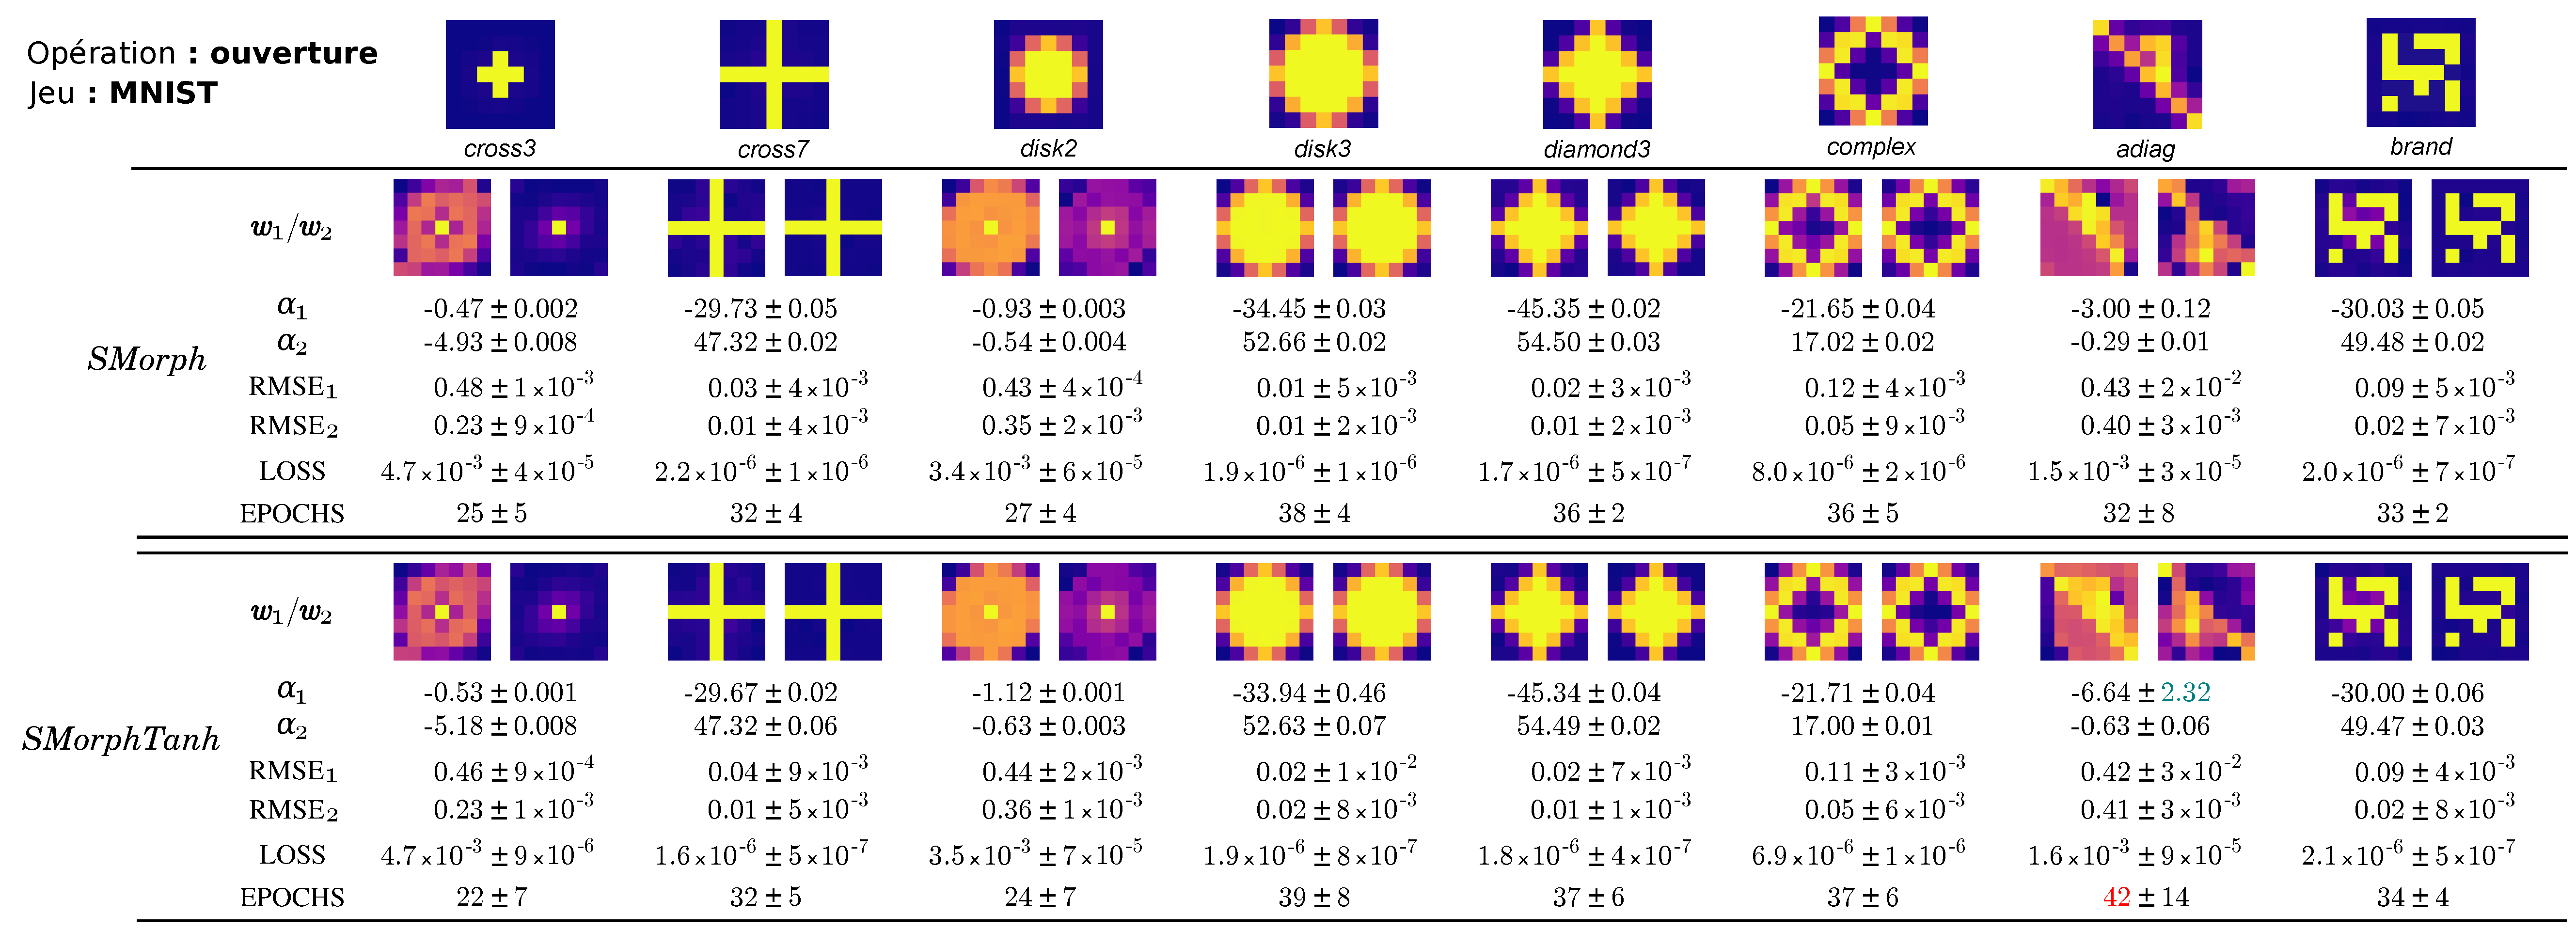
\includegraphics[width=1.00\textwidth]{parts/3-contributions/A-reseaux_smorphTANH/figures/t_opening_mnist.pdf}
    \vspace{-2.0mm}
    \caption{ \centering Comparaison des poids appris et des moyennes et écarts-types des métriques $\alpha$, \textit{RMSE}, \textit{loss} et nombre d'époques, et ce sur six runs, entre $\mathcal{S}$Morph et $\mathcal{S}$MorphTanh à deux couches, pour les huit fonctions structurantes cibles et l'opération d'\textbf{ouverture}.}
    \label{fig:SMvsSMTH_opening_mnist}
  \end{center}
\end{figure}


\newpage

%Pour l'opération cible de fermeture sur des réseaux à deux couches morphologiques, on obtient les résultats suivants : \\
Pour la fermeture sur réseaux à deux couches, on obtient les résultats suivants : \\

% figure
\vspace{2.0mm}
\begin{figure}[ht]
  \begin{center}
    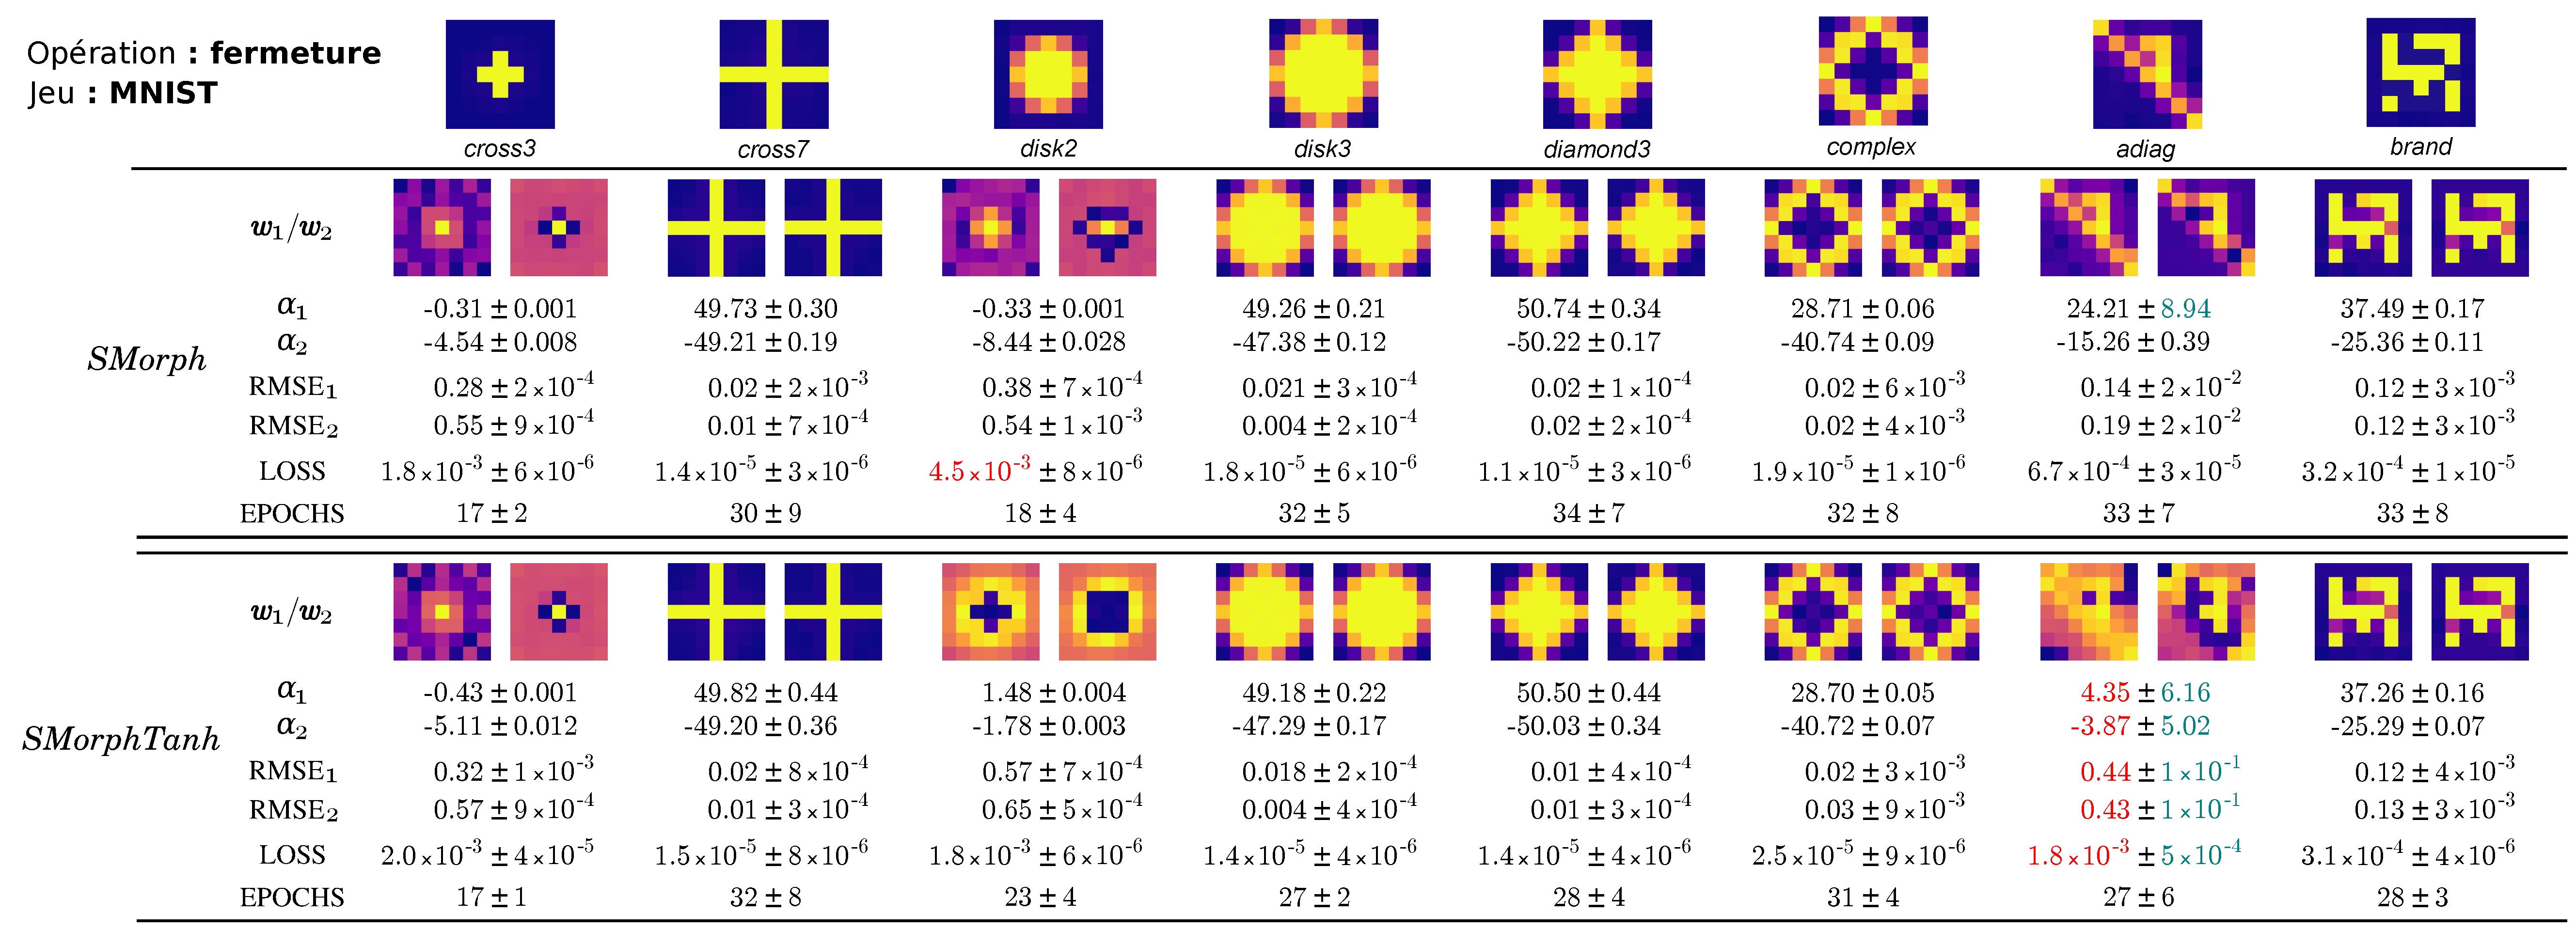
\includegraphics[width=1.00\textwidth]{parts/3-contributions/A-reseaux_smorphTANH/figures/t_closing_mnist.pdf}
    \vspace{-2.0mm}
    \caption{ \centering Comparaison des poids appris et des moyennes et écarts-types des métriques $\alpha$, \textit{RMSE}, \textit{loss} et nombre d'époques, et ce sur six runs, entre $\mathcal{S}$Morph et $\mathcal{S}$MorphTanh à deux couches, pour les huit fonctions structurantes cibles et l'opération de \textbf{fermeture}.}
    \label{fig:SMvsSMTH_closing_mnist}
  \end{center}
\end{figure}


\vspace{-3.2mm}

\vspace{-1.6mm}
Pour les réseaux à une couche : 
il n'existe pas de grandes différences entre les résultats portés par $\mathcal{S}$MorphNet et ceux portés par $\mathcal{S}$MorphNetTanh. L'ensemble des résultats semble plutôt bon pour ces deux réseaux uni-couche, aussi bien au niveau de la \textit{loss}, de la \textit{RMSE}, du signe et de l'amplitude de $\alpha$, et de la vitesse de convergence. Il existe toutefois deux expériences dont les résultats entre ces deux réseaux divergent légèrement : la première avec \textit{cross3} où $\mathcal{S}$MorphNetTanh semble meilleur en terme de \textit{RMSE} et de \textit{loss} ; la seconde avec \textit{adiag} où cette fois $\mathcal{S}$MorphNet semble meilleur. \\

\vspace{-1.8mm}
\noindent Pour les réseaux à deux couches : 
on retrouve les mêmes problèmes de convergence avec \textit{cross3} et \textit{disk2} que dans l'état de l'art (partie 2.4). On remarque que \textit{adiag} pose ici également des problèmes pour les deux réseaux. Cependant, là où $\mathcal{S}$MorphNet et $\mathcal{S}$MorphNetTanh se comportent de la même manière sur ces trois structures cibles avec l'ouverture, ils se comportent plutôt différemment avec la fermeture. Pour les autres structures, les deux réseaux donnent des résultats à la fois bons et similaires. \\

\vspace{-1.8mm}
\noindent Ces expériences ont été réalisées avec une autre banque d'images, FashionMNIST, et les mêmes conclusions de similarité d'efficacité des deux réseaux ont pu être établies. \\
%malgré quelques divergences

En conclusion, 
les deux modèles ont une précision et une vitesse de convergence similaires. 
Quelques rares différences dans les résultats subsistent sur certaines expériences, autant en faveur de $\mathcal{S}$MorphNetTanh qu'en sa défaveur. 
%Parmi ces différences notables, autant sont en faveur de $\mathcal{S}$MorphNetTanh qu'en sa défaveur. 
$\mathcal{S}$MorphTanh est donc équivalent à $\mathcal{S}$Morph en terme de performances. Il résout néanmoins le problème de signe devant $w$ dans la formulation asymptotique de $\mathcal{S}$Morph lorsque $\alpha \rightarrow -\infty$. On gardera alors le $\mathcal{S}$MorphNetTanh comme réseau d'étude pour la suite.

\newpage

% Partage de poids
\subsection{Partage de poids} %Partage de poids

\subsubsection{Contexte et motivations}
\vspace{0.2cm}
Les résultats précédents montrent qu'il reste encore quelques cas d'échecs de convergence pour les réseaux $\mathcal{S}$MorphNetTanh à deux couches morphologiques, avec les opérations cibles d'ouverture et de fermeture, et ce malgré l'ajout d'un partage doux des poids entre les noyaux $w$ des deux couches et l'ajout dans la \textit{loss} d'une contrainte $C_\text{awayOPP}$ entre les deux paramètres de contrôle $\alpha$ (ou $p$) associés. \\

\vspace{-1.4mm}
\noindent La modulation de l'initialisation des noyaux $w$ du réseau devient alors une solution potentielle à ces derniers échecs. ALors que les poids des noyaux sont originellement initialisés selon une loi normale centrée réduite afin de brasser les différents états de convergence possibles à partir d'initialisations aléatoires différentes sur plusieurs expériences, on peut finalement se dire que cette forme initiale des noyaux peut être fixée et définie de manière déterminée au préalable, selon des caractéristiques morphologiques générales à priori que l'on connait ou que l'on recherche sur ces noyaux. \\

\vspace{-1.4mm}
\noindent En l'occurence, on peut facilement s'imaginer que ce que l'on recherche ou favorise dans nos différents cas d'étude, c'est une forme de noyaux centrée sur son support et peu dispersée. On choisira alors une initialisation sous la forme d'une gaussienne 2D, allant de $0$ aux coins de l'image des noyaux à $1$ en son centre (voir figure \ref{fig:init_gauss} suivante). \\


%figure
\vspace{-1.0mm}
\begin{figure}[htp]
  \begin{center}
    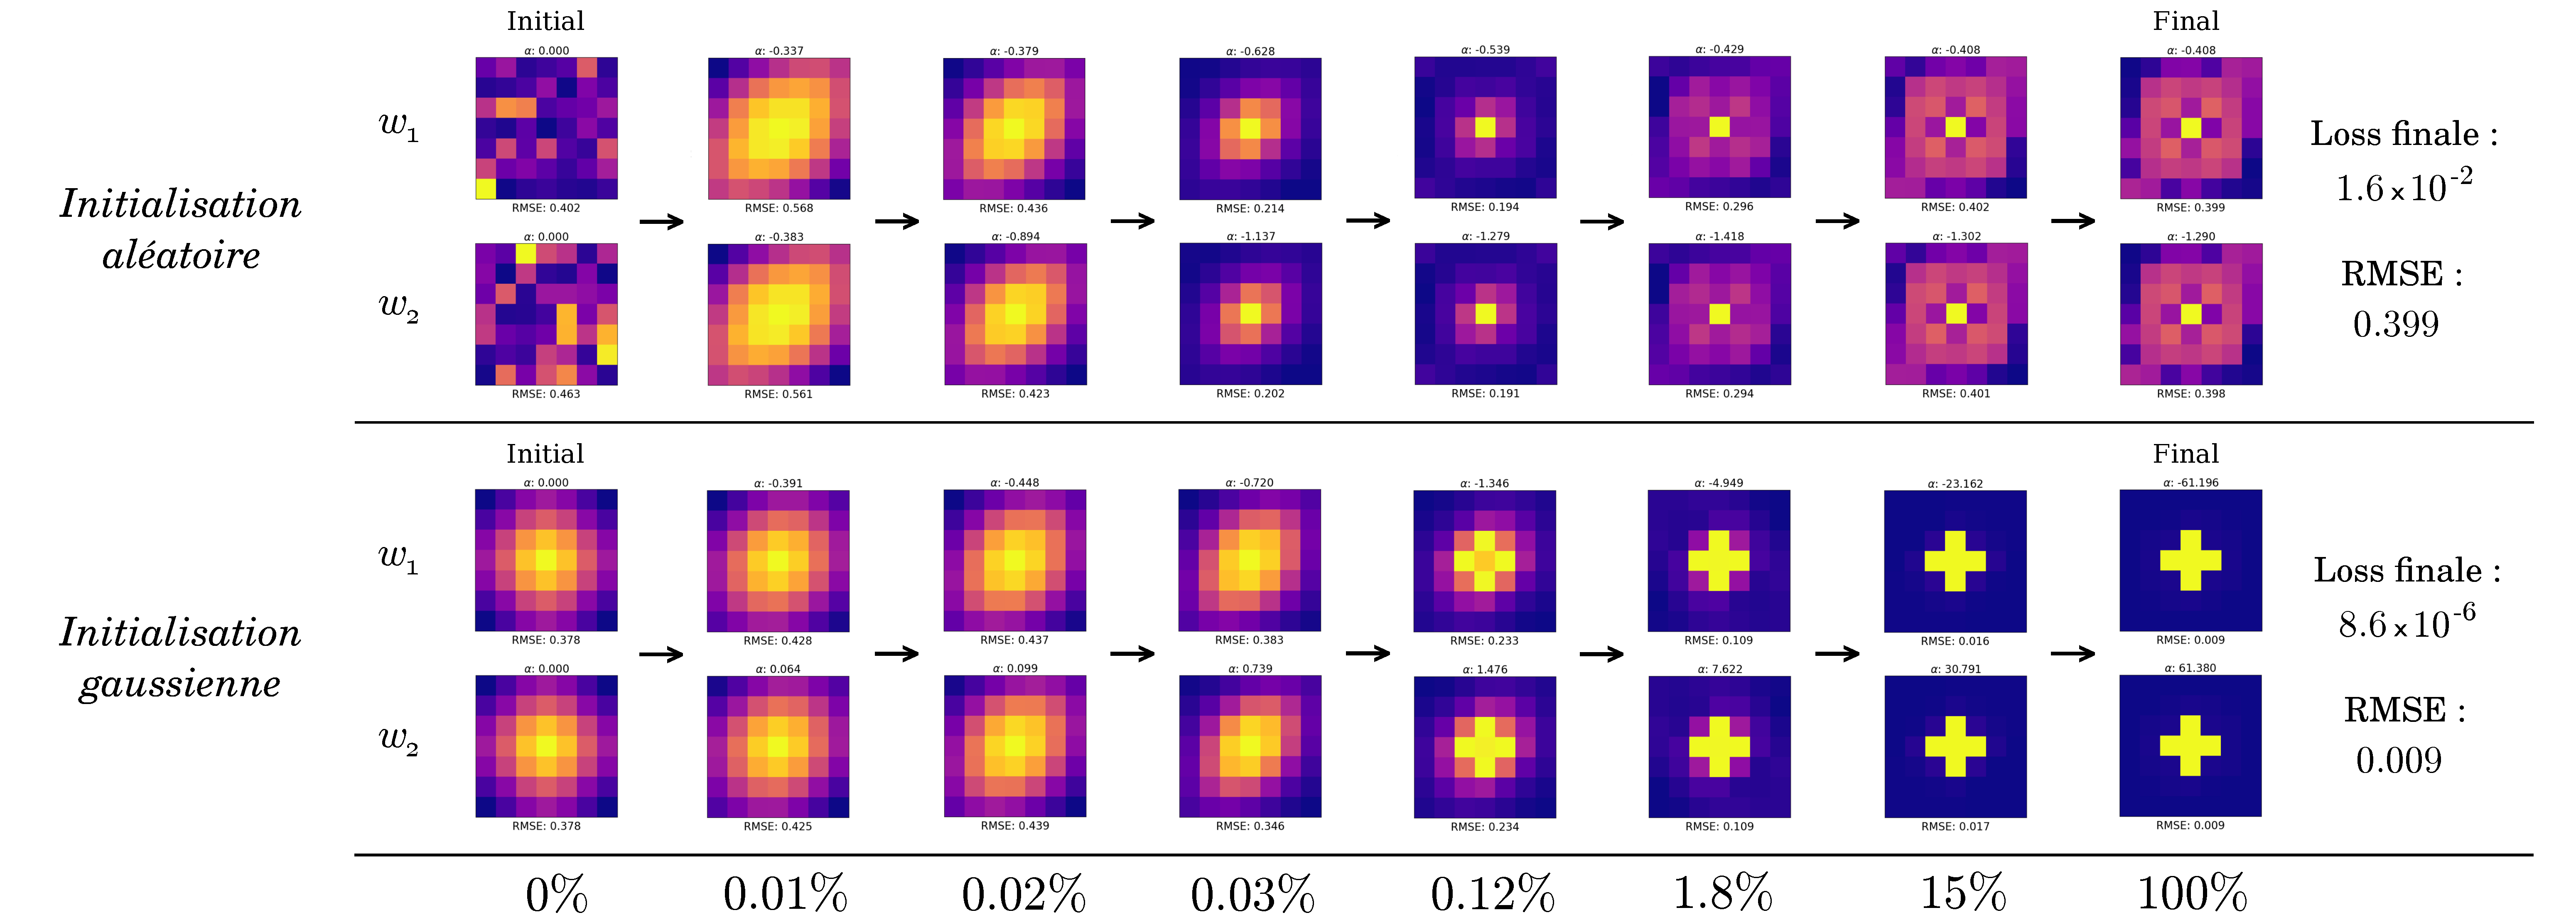
\includegraphics[width=1.00\linewidth]{parts/3-contributions/D-modulation_de_l_initialisation/figures/k_gauss.pdf}
    \vspace{-4.0mm}
    \caption{ \centering Évolution de la forme du noyau des deux couches du réseau et de sa \textit{RMSE} en fonction de la progression de l'entraînement (en \% avant l'état final), pour le \textit{cross3} et l'ouverture sur la banque MNIST, avec initialisation aléatoire et init. gaussienne.}
    \label{fig:init_gauss}
  \end{center}
\end{figure}


\vspace{-3.0mm}
\noindent L'exemple fig. \ref{fig:init_gauss}, obtenu sur six runs, montre bien ici l'efficacité de cette initialisation gaussienne des noyaux $w$ par rapport à l'aléatoire normale centrée réduite sur \textit{cross3} pour l'ouverture sur MNIST, avec des valeurs de \textit{RMSE} et de \textit{loss} bien plus faibles.

\newpage

\subsubsection{Partage de poids dur}
\vspace{0.2cm}
La méthode de partage de poids dite << dure >> fait un partage direct des poids du noyau de la première couche avec ceux du noyau de la seconde couche du réseau. Les deux couches ayant ainsi exactement le même noyau, on peut les considérer comme une seule et même couche, dite << duale >>, mais avec bien deux paramètres de contrôle indépendants, notés $\alpha_1$ et $\alpha_2$. 
%, par appliquer successivement deux fois le filtre $w$ de manière contrôlée différente sur l'image d'entrée de couche. 
Ces dernières permettent aux poids du même noyau $w$ d'être appliqués deux fois successivement mais de manière différente à l'image en entrée de couche, la première fois sous le contrôle de $\alpha_1$, la seconde fois sous celui de $\alpha_2$. \\

\vspace{-1.6mm}
\noindent Cependant, d'après les formules aux limites de $\mathcal{S}$MorphTanh (p. 22), il est nécessaire de considérer la symétrie de $w$ quelque part lorsque $\alpha_1$ et $\alpha_2$ sont de signe opposé, et donc pour que le réseau puisse effectivement converger vers une ouverture ou une fermeture de $f$ par $w$. On va d'abord considérer la formule de $\mathcal{S}$MorphTanh sous symétrie conditionnelle, notée $\mathcal{S}\text{MT}_{\text{cond}}$, qui est définie pour toute image $f: I \subseteq \mathbb{Z}^2 \rightarrow \mathbb{R}$, tout noyau $w: W \subseteq \mathbb{Z}^2 \rightarrow \mathbb{R}$ et tout réel $\alpha \in \mathbb{R}$ de la manière suivante (\ref{SMorphTanh_condi}) : \\

\vspace{-5.0mm}
\begin{equation}
    \mathcal{S}\text{MT}_{\text{cond}} (f,w,\alpha) = 
    \begin{cases}
        \hspace{1.4mm} \mathcal{S}\text{MorphTanh} (f,w,\alpha) & \mbox{si} \hspace{3mm} \alpha \geqslant 0 \\
        \hspace{1.4mm} \mathcal{S}\text{MorphTanh} (f,\breve{w},\alpha) & \mbox{sinon}
    \end{cases}
    \label{SMorphTanh_condi}
\end{equation}

\vspace{2.5mm}
\noindent Malgré la conditionnalité sur $\alpha$ dans la définition de la fonction $\mathcal{S}\text{MT}_{\text{cond}}$, la transition du noyau $w$ à sa symétrique, quand $\alpha$ passe d'un signe négatif à un signe positif ou inversement dans la formule de $\mathcal{S}$MorphTanh, reste lisse, rendant $\mathcal{S}\text{MT}_{\text{cond}}$ continue (mais pas forcément dérivable) en $\alpha = 0$, grâce au $\tanh{(\alpha)}$ devant $w$. \\

\vspace{-1.0mm}
La fonction de transformation de la couche $\mathcal{S}$MorphTanhDual est ainsi définie, pour toute image $f: I \subseteq \mathbb{Z}^2 \rightarrow \mathbb{R}$ et tout noyau de couche $w: W \subseteq \mathbb{Z}^2 \rightarrow \mathbb{R}$, et avec $\alpha_1,\alpha_2 \in \mathbb{R}$, par : \\

\vspace{-4.0mm}
\begin{equation}
    \pmb{\mathcal{S}}\textbf{MorphTanhDual} (f,w,\alpha_1,\alpha_2) = \mathcal{S}\text{MT}_{\text{cond}} \left ( \mathcal{S}\text{MT}_{\text{cond}} ( f , w , \alpha_1 ) , w , \alpha_2 \right )
    \label{SMorphTanhDual}
\end{equation}

\vspace{5mm}
\noindent Ainsi, si $\alpha_1$ et $\alpha_2$ ont un signe opposé, on obtient l'ouverture (si $\alpha_1 \ll 0$ et $\alpha_2 \gg 0$) ou la fermeture (si $\alpha_1 \gg 0$ et $\alpha_2 \ll 0$) de l'image $f$ par la fonction structurante $w$. \\

\vspace{-1.6mm}
\noindent On a donc les limites asymptotiques de $\mathcal{S}$MorphTanhDual suivantes : \\

%formules asymptotiques avec ouverture et fermeture
\vspace{-5.0mm}
\begin{equation*} 
    \lim_{\substack{\alpha_1 \rightarrow -\infty \\ \alpha_2 \rightarrow +\infty}} \mathcal{S}\text{MorphTanhDual}(f,w,\alpha_1,\alpha_2) = f \circ w
\end{equation*} 
\begin{equation*} 
    \lim_{\substack{\alpha_1 \rightarrow +\infty \\ \alpha_2 \rightarrow -\infty}} \mathcal{S}\text{MorphTanhDual}(f,w,\alpha_1,\alpha_2) = f \bullet w
\end{equation*}

\vspace{2.5mm}
\noindent On obtient bien avec $\mathcal{S}$MorphTanhDual, aux limites, l'ouverture et la fermeture.

\newpage

\subsubsection{Partage de poids doux}
\vspace{0.2cm}
La méthode de partage de poids dite « douce », quant à elle, ne modifie pas la structure-même du réseau.
Elle se base sur l'expression d'une métrique de contrainte entre les poids des noyaux des deux couches morphologiques du réseau, qui est alors ajoutée dans la fonction de perte globale \textit{loss}, et qui va ainsi faire tendre ces deux noyaux symétriquement vers la même forme durant l'entraînement du réseau, sans donc passer par un transfert direct dur des poids d'une couche à l'autre. 
La contrainte fait ainsi prendre la même forme aux deux noyaux, mais de manière plus douce. \\
%La << puissance >> de cette contrainte par rapport aux autres métriques dans la \textit{loss} est modulée par un hyperparamètre noté $\lambda$. \\

\vspace{-2.0mm}
Rappelons d'abord la formule de l'erreur quadratique moyenne (MSE) entre deux fonctions $f_1$ et $f_2$ définies sur le même ensemble dénombrable $I$ à valeurs dans $\mathbb{R}$, qui est utilisée dans notre cas pour calculer l'éloignement entre deux images : \\

\vspace{-4.4mm}
\begin{equation}
    \text{MSE} (f_1,f_2) = \mathbb{E} \left ( (f_2-f_1)^2 \right ) = \frac{1}{|I|} \sum_{x \in I} \left ( f_2(x) - f_1(x) \right ) ^2
    \label{MSE}
\end{equation}

\vspace{2.5mm}
La fonction de perte \textit{loss} du réseau, qui permet d'entraîner et d'évaluer les performances de prédiction de ce dernier, se formule classiquement comme la MSE entre les images cibles $F_\text{cible}$ et les images prédites par le réseau $F_\text{pred}$ : $\textit{loss} = \text{MSE}(F_\text{cible},F_\text{pred})$. 
Dans la \textit{loss}, est alors ici ajoutée à $\text{MSE}(F_\text{cible},F_\text{pred})$ une contrainte de similarité $C_\text{sim}$ entre le noyau de la première couche, $w_1$, et celui de la seconde, $w_2$. 
Cette contrainte est pondérée par l'hyperparamètre $\lambda$ qui permet de moduler son influence dans la convergence du réseau lors de l'entraînement, par rapport à celle de $\text{MSE}(F_\text{cible},F_\text{pred})$. \\

\vspace{-2.0mm}
\noindent On étudie trois formulations de cette métrique de contrainte entre $w_1$ et $w_2$. Elles sont explicitées à la page suivante. Pour mieux les comprendre, définissons d'abord deux fonctions de rééchelonnage linéaire primaires, la normalisation et la standardisation. \\

\vspace{0.0mm}
On définit la << normalisation >> comme la fonction $\mathfrak{N}_{(a,b)}$ qui à une image $f: I \rightarrow \mathbb{R}$ associe son rééchelonnage linéaire (rescale) dans un intervalle $[a,b] \subset \mathbb{R}$ : \\

\vspace{-3.5mm}
\begin{equation}
    \mathfrak{N}_{(a,b)} (f) = \frac{f-\inf_{x \in I}\{f(x)\}}{\sup_{x \in I}\{f(x)\}-\inf_{x \in I}\{f(x)\}} \left ( b-a \right ) + a
    \label{normalized}
\end{equation}

\vspace{4.5mm}
On définit la << standardisation >> comme la fonction $\mathfrak{S}$ qui à une image $f: I \rightarrow \mathbb{R}$ associe son rééchelonnage linéaire de moyenne $\mathbb{E}(\mathfrak{S}(f)) = 0$ et d'écart-type $\sigma(\mathfrak{S}(f)) = 1$ sur l'ensemble de ses valeurs d'arrivée $f(I)$ : \\

\vspace{-4.0mm}
\begin{equation}
    \mathfrak{S} (f) = \frac{f-\mathbb{E}(f)}{\sigma(f)} = \frac{ f - \frac{1}{|I|} \sum_{x \in I} f(x) }{ \sqrt{ \frac{1}{|I|} \sum_{x \in I} \left ( f(x) - \frac{1}{|I|} \sum_{x \in I} f(x) \right ) ^2 } }
    \label{standardized}
\end{equation}


\newpage

\noindent \textbf{a. Première formulation} \\

\vspace{-1.5mm}
%, avec les poids du noyau $w_1$ de la première couche du réseau et ceux du noyau $w_2$ de la seconde couche,
La première formulation de la métrique de contrainte $C_\text{sim}$ est définie à partir de la MSE entre les deux noyaux $w_1$ et $w_2$, symétrisés l'un par rapport à l'autre et normalisés (\ref{normalized}) entre 0 et 1. Ainsi, $C_\text{sim}$ est définie pour tous noyaux $w_1$ et $w_2$ par : \\

\vspace{-4.7mm}
\begin{equation}
    C_\text{sim}(w_1,w_2) = \text{MSE} \left ( \mathfrak{N}_{(0,1)}(w_1) , \mathfrak{N}_{(0,1)}(\breve{w_2}) \right )
    \label{Csim1}
\end{equation}

\vspace{3.5mm}
\noindent \textbf{b. Deuxième formulation} \\

\vspace{-1.5mm}
%, avec les poids du noyau $w_1$ de la première couche du réseau et ceux du noyau $w_2$ de la seconde couche,
La deuxième formulation de la métrique de contrainte $C_\text{sim}$ est définie à partir de la MSE entre les deux noyaux $w_1$ et $w_2$, symétrisés l'un par rapport à l'autre et cette fois standardisés (\ref{standardized}). Ainsi, $C_\text{sim}$ est définie pour tous noyaux $w_1$ et $w_2$ par : \\

\vspace{-4.7mm}
\begin{equation}
    C_\text{sim}(w_1,w_2) = \text{MSE} \left ( \mathfrak{S}(w_1) , \mathfrak{S}(\breve{w_2}) \right )
    \label{Csim2}
\end{equation}

\vspace{3.5mm}
\noindent \textbf{c. Troisième formulation} \\

\vspace{-1.5mm}
%, entre les poids du noyau $w_1$ de la première couche du réseau et ceux du noyau $w_2$ de la seconde couche,
La troisième formulation de la métrique de contrainte $C_\text{sim}$ est définie à partir de la MSE entre les deux noyaux $w_1$ et $w_2$, symétrisés l'un par rapport à l'autre et standardisés, mais multipliés par l'écart-type des poids d'un des deux noyaux, afin d'éviter de changer et d'influencer, avec un écart relatif, la taille de la gamme des poids des noyaux. $C_\text{sim}$ est alors définie pour tous noyaux $w_1$ et $w_2$ par : \\

\vspace{-4.7mm}
\begin{equation}
    C_\text{sim}(w_1,w_2) = \text{MSE} \left ( \hspace{1mm}  w_1 - \mathbb{E}(w_1) \hspace{1.5mm},\hspace{1.5mm} ( \breve{w_2} - \mathbb{E}(\breve{w_2}) ) \frac{\sigma(w_1)}{\sigma(\breve{w_2})}  \hspace{1mm} \right )
    \label{Csim3}
\end{equation}

\vspace{3.6mm}
\noindent \textbf{Remarque :} \\

\vspace{-1.5mm}
\noindent Si on prend ici la symétrique de $\breve{w_2}$ de $w_2$, c'est parce que, comme précédemment, le problème de symétrie dans l'expression asymptotique de la formule de $\mathcal{S}$MorphTanh (p. 22) nécessite de prendre la symétrie d'un des deux noyaux $w$. 
De plus, si les trois formulations se basent sur un rééchelonnage des noyaux, c'est parce qu'ils peuvent tous deux s'exprimer dans deux intervalles de $\mathbb{R}$ très différents liés à la standardisation en entrée du réseau et au filtre de convolution de taille 1 en sortie. On imagine alors qu'il doit exister une relation linéaire entre la disposition dans $\mathbb{R}$ des poids du premier noyau $w_1$ et la disposition dans $\mathbb{R}$ de ceux du second noyau $w_2$. \\

\vspace{-0.1mm}
\noindent Avec $C_\text{sim}$ définie par l'une des trois formulations présentées (\ref{Csim1}, \ref{Csim2}, \ref{Csim3}), la nouvelle formule de la \textit{loss} dans le cadre de ce partage de poids doux s'écrit ainsi : \\

\vspace{-4.0mm}
\begin{equation}
    \textit{loss} = \text{MSE} \left ( F_\text{cible},F_\text{pred} \right ) + \lambda \times C_\text{sim}(w_1,w_2)
    \label{MSEpConstraintFilters}
\end{equation}


\newpage

\noindent \textbf{Comparaison rapide de résultats de convergence entre ces trois formulations} \\

Pour savoir quelle formulation de la contrainte de similarité $C_\text{sim}$ entre $w_1$ et $w_2$ est la plus adaptée à nos besoins, on exécute plusieurs expériences d'entraînement de réseau $\mathcal{S}$MorphNetTanh à deux couches, avec séparément les trois différentes formulations de $C_\text{sim}$ telles que décrites précédemment, ajoutées dans la \textit{loss}. On observe alors rapidement la forme des deux noyaux $w_1$ et $w_2$ après convergence du réseau. La figure suivante présente les résultats, associés par paires (la première image pour $w_1$, la seconde qui suit pour $w_2$), sur l'ensemble des expériences avec les huit structures cibles, et deux banques d'images (MNIST et FashionMNIST). \\

%figure
\vspace{-0.5mm}
\begin{figure}[ht]
  \begin{center}
      \subfigure[Avec la 1ère formulation]{
          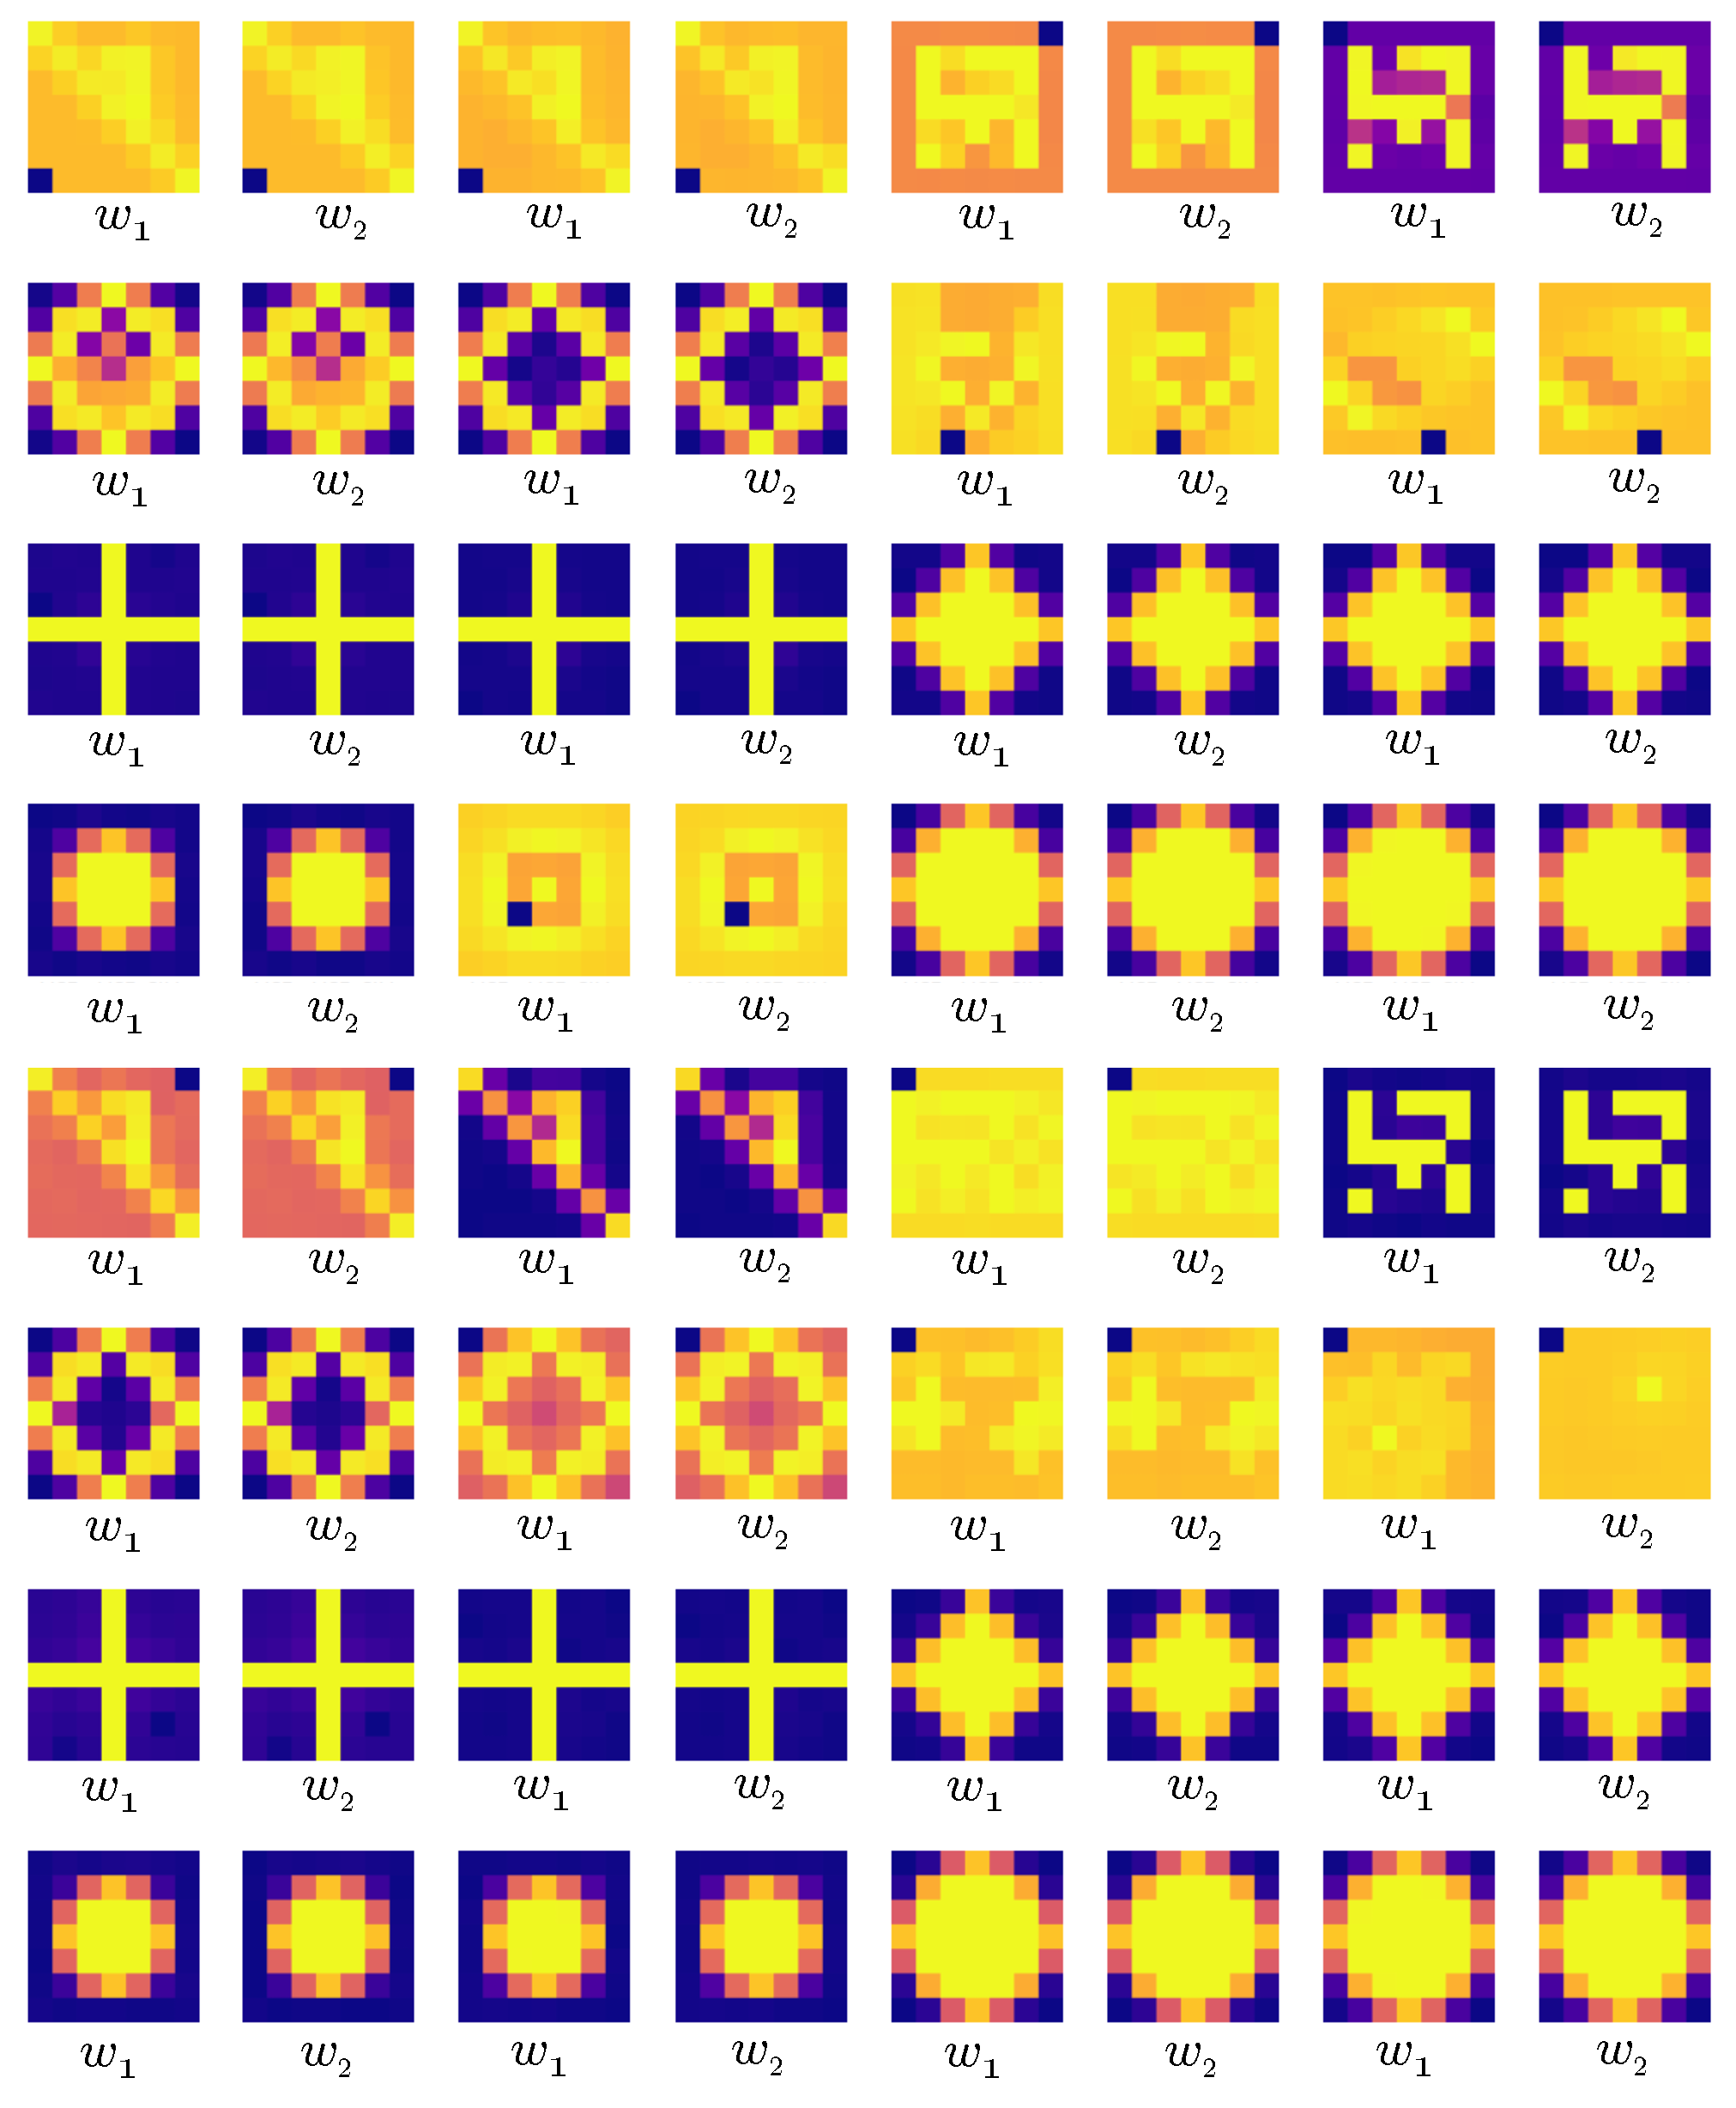
\includegraphics[width=0.31\textwidth]{parts/3-contributions/B-partage_de_poids/figures/quick_visu_NORM.pdf}
          \label{fig:nor1}}\hfill
      \subfigure[Avec la 2ème formulation]{
          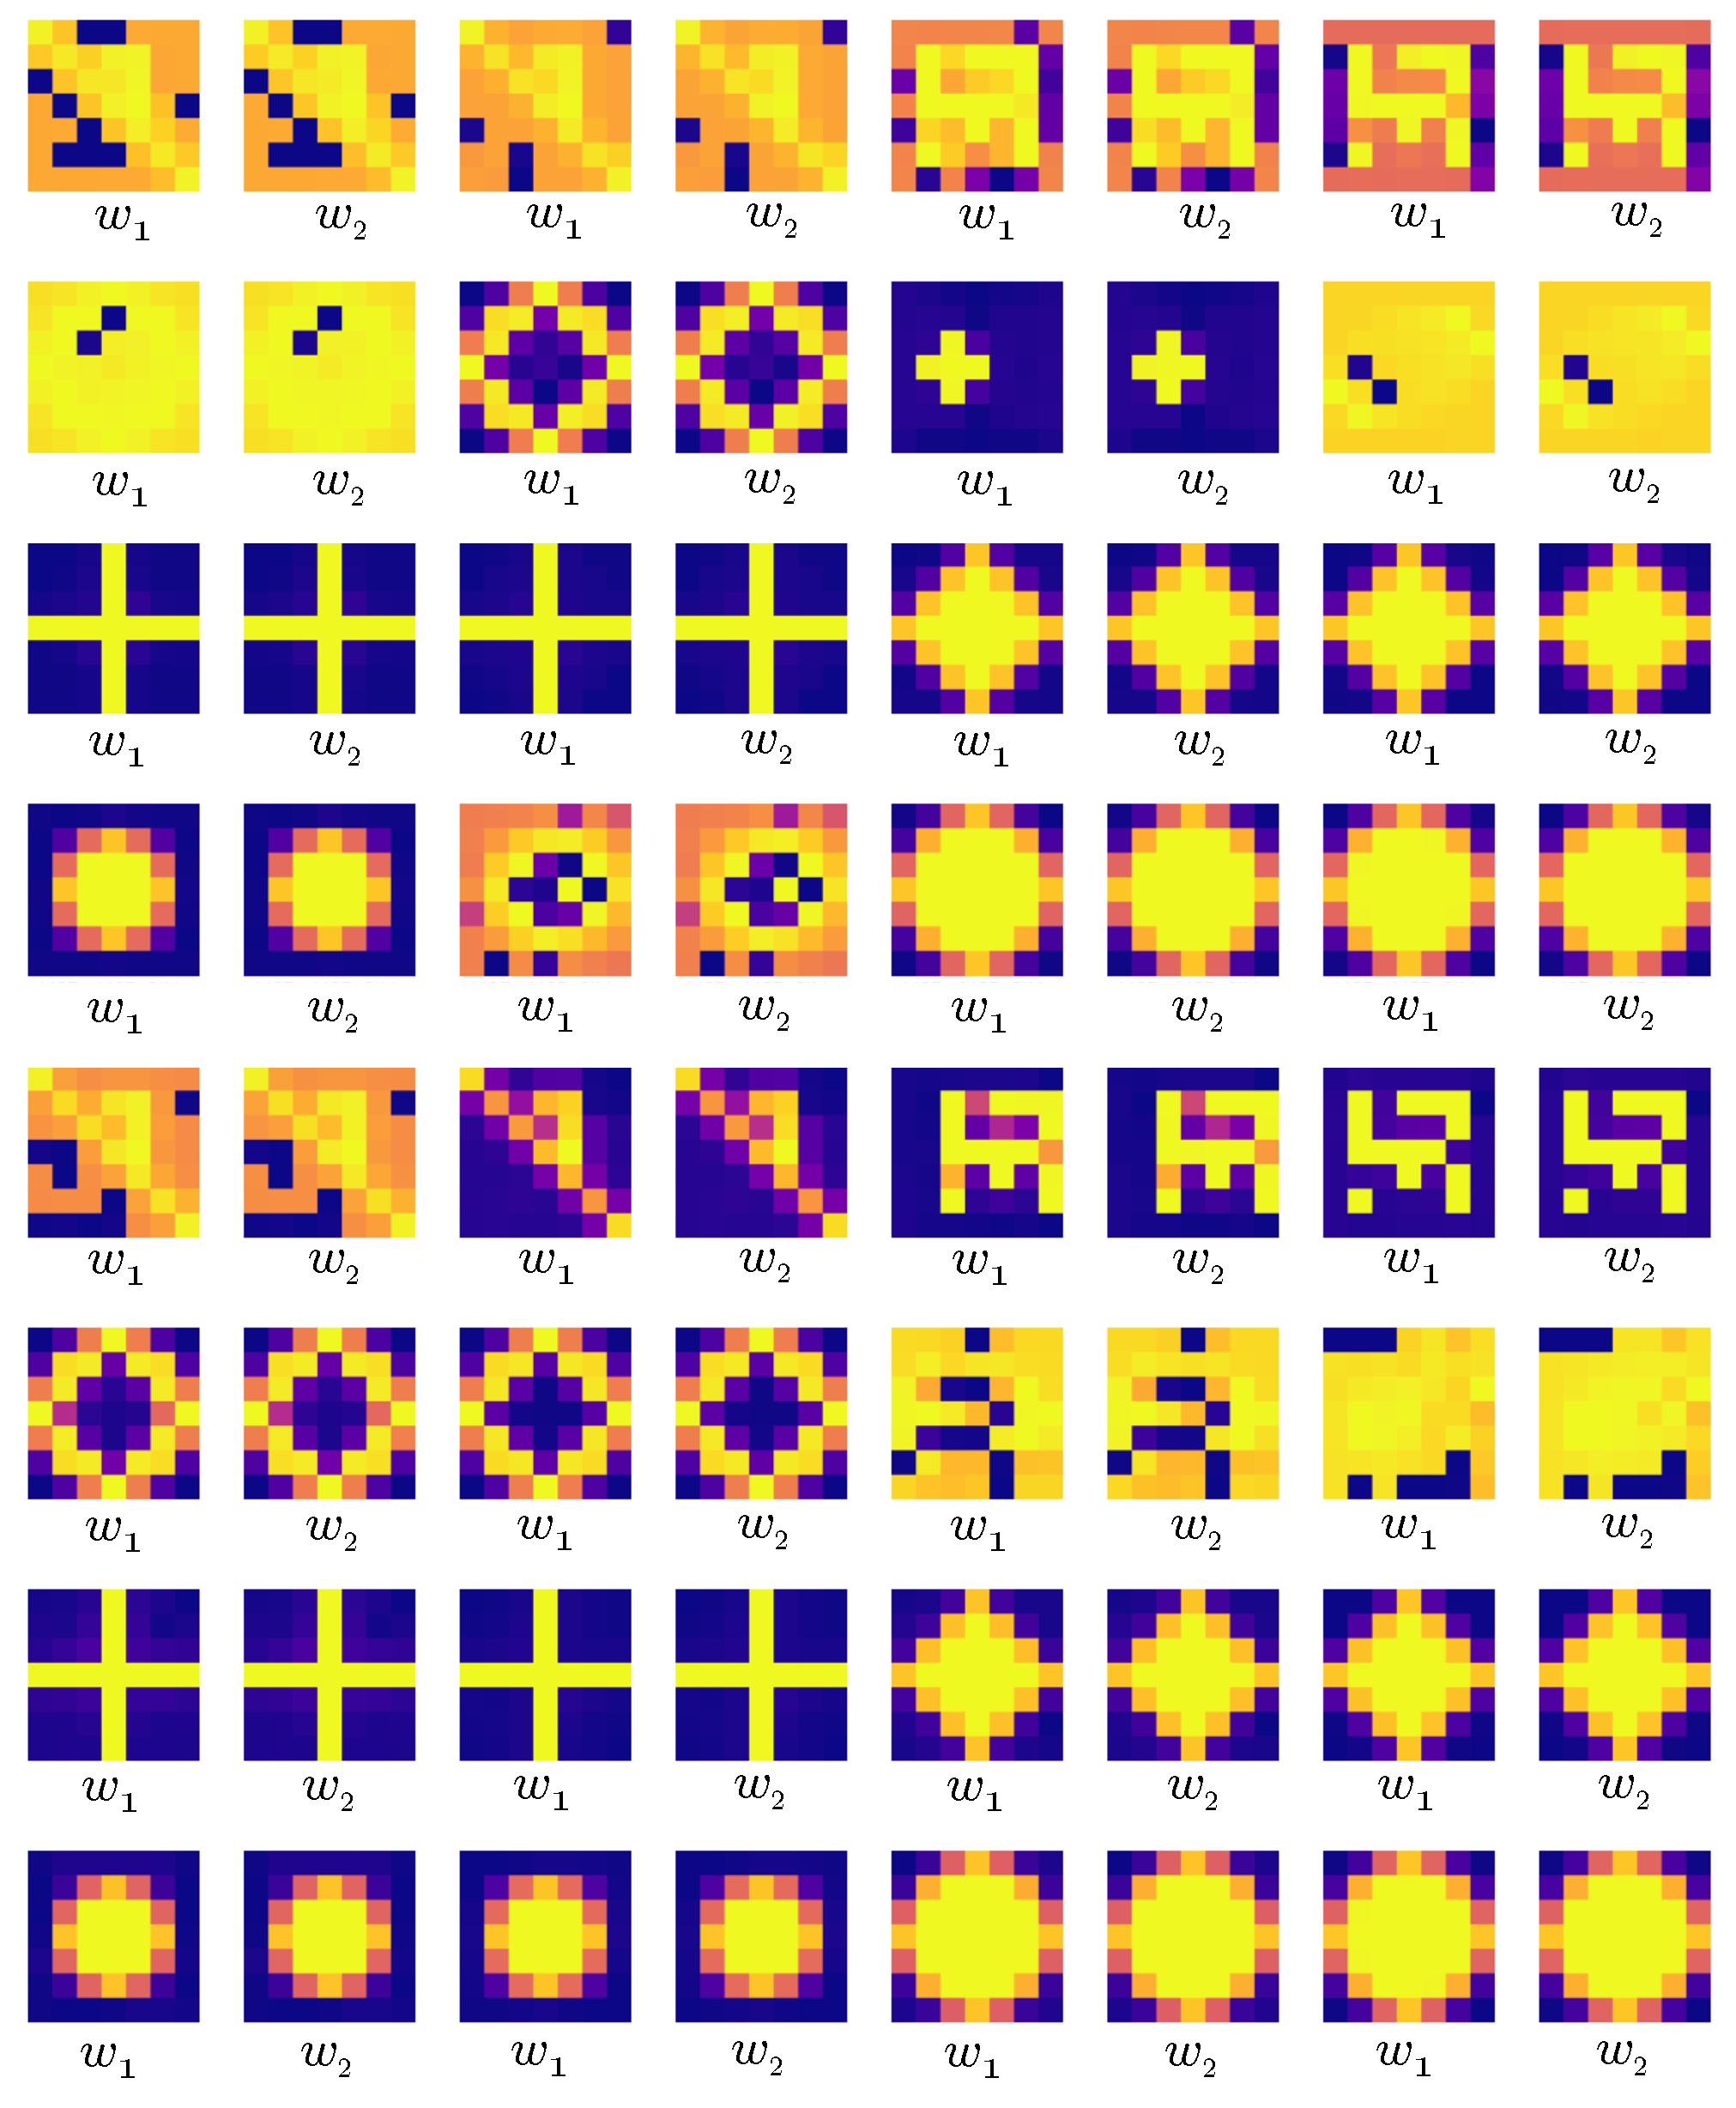
\includegraphics[width=0.31\linewidth]{parts/3-contributions/B-partage_de_poids/figures/quick_visu_STAND.pdf}
          \label{fig:nor2}}\hfill
      \subfigure[Avec la 3ème formulation]{
          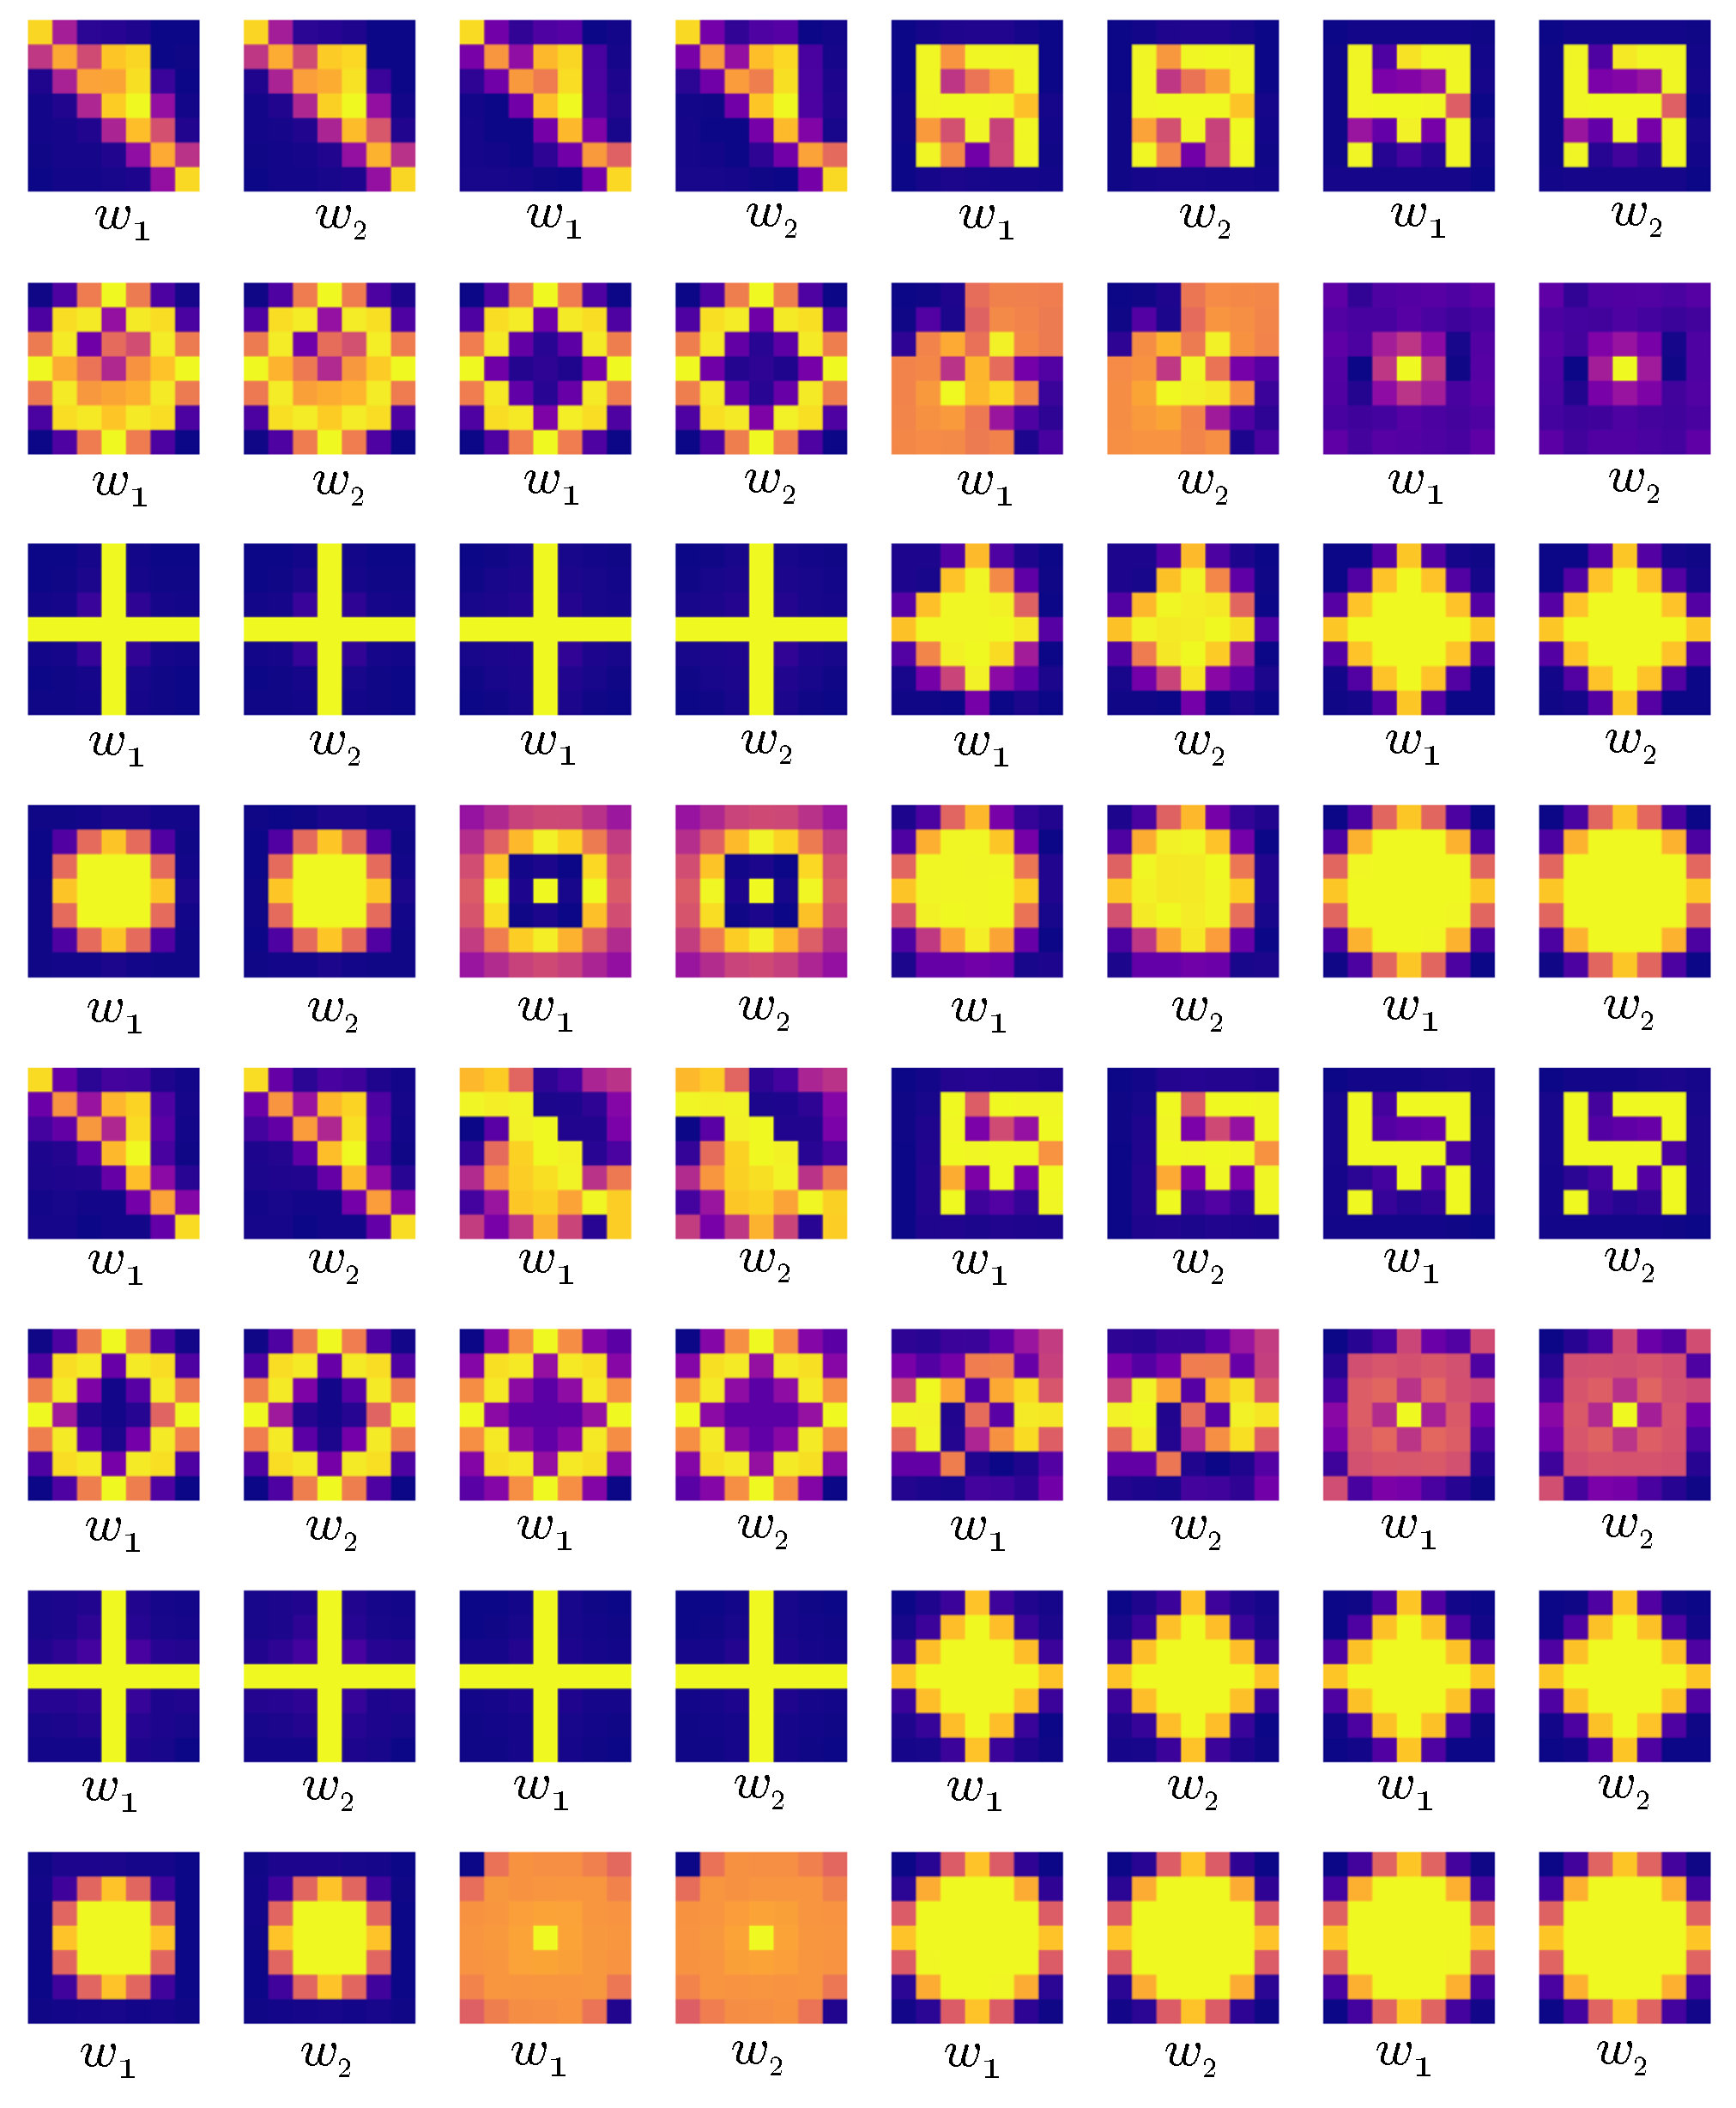
\includegraphics[width=0.31\textwidth]{parts/3-contributions/B-partage_de_poids/figures/quick_visu_TRUE.pdf}
          \label{fig:nor3}}
    \caption{ \centering Forme des noyaux $w_1$ et $w_1$ par paires du réseau $\mathcal{S}$MorphNetTanh à deux couches après convergence, sur un ensemble de 32 expériences, avec dans la \textit{loss} la première formulation de $C_\text{sim}$ (\ref{fig:nor1}), la deuxième (\ref{fig:nor2}) et la troisième (\ref{fig:nor3}).}
    \label{fig:quick_visualisation_contraintes_partage_de_poids}
  \end{center}
\end{figure}

\vspace{-3.5mm}
Sur la figure, chaque emplacement d'un résultat d'une des trois cartes à l'autre représente la même expérience.
On remarque tout de suite le problème avec la première formulation \ref{fig:nor1} basée sur la normalisation (\ref{normalized}) : elle a tendance a binariser les filtres sur certaines expériences (première ligne, les deux premières paires par exemple), en éloignant un unique pixel très bas dans les valeurs (en bleu foncé, jusqu'à -80). Mais cela n'est que visuel, il n'y a pas d'impact sur l'opération car, en dessous d'un certain seuil, toute valeur a le même effet que $-\infty$.
De même pour la seconde formulation \ref{fig:nor2} basée, elle, sur la standardisation (\ref{standardized}). Cependant, elle a tendance à éloigner plusieurs pixels très bas dans les valeurs, plutôt qu'un unique pixel. Quant à la troisième, il n'y a pas ce problème de binarisation, car pas de mise en échelle des gammes. Elle donne les résultats qu'on attendait, similaires à ceux avec la \textit{loss} sans contrainte, mais avec les deux noyaux de chaque paire qui tendent bien vers la même forme. 


%%% Suite page suivante!!

\newpage

On remarque néanmoins que, sur certaines expériences, là où la troisième formulation donne les mêmes mauvais résultats (échecs) de convergence que les expériences sans contrainte dans la \textit{loss} (uniquement la MSE entre les images cibles et les prédictions), les deux autres formulations permettent au réseau de trouver la vraie fonction structurante cible pour ces quelques expériences cibles-là (par exemple, avec le \textit{disk2} en fermeture pour MNIST, dernière ligne et deuxième paire à partir de la gauche).\\

\vspace{-2.0mm}
\noindent Ces bons résultats des deux premières formulations (\ref{Csim1} et \ref{Csim2}), qui surpassent la troisième (\ref{Csim3}) sur ces quelques échecs de convergence, semblent liés au rééchelonnage de la gamme de valeurs des poids $w_1$ et $w_2$, qui fait qu'un éloignement d'une partie des valeurs entraîne une binarisation de ces dernières, qui réduit alors drastiquement la valeur de la contrainte $C_\text{sim}(w_1,w_2)$. Ils pourront être considérés plus tard dans le cadre de l'amélioration de la convergence des réseaux sur ces expériences-là. \\

\vspace{-2.0mm}
\noindent On préfèrera la troisième formulation dans cette optique de partage de poids doux, car seule cette dernière a le comportement que l'on visait initialement, c'est-à-dire faire uniquement tendre les deux noyaux vers la mêmes forme sans créer d'éloignement de valeurs et de binarisation, pour ensuite voir les résultats d'une telle contrainte et estimer si elle permet à elle seule une amélioration de la convergence des réseaux.

%\newpage

\subsubsection{Comparaison de l'efficacité}
\vspace{0.2cm}
Pour comparer l'efficacité des partages de poids dur et doux, on reprend le même protocole et les mêmes expériences que précédemment avec $\mathcal{S}$MorphNetTanh : on considère les quatre mêmes métriques d'évaluation de la performance des réseaux (\textit{loss}, \textit{RMSE}, valeurs de $\alpha_1$ et $\alpha_2$, et nombre d'époques pour converger) ; on reprend la banque d'images en niveaux de gris MNIST (on fait également, à part, les expériences sur FashionMNIST) ; on fait toujours six runs par expérience ; et on considère enfin les huit fonctions structurantes cibles telles qu'illustrées sur les figures suivantes. \\
%méthodologie

\vspace{-2.0mm}
\noindent Dans le cas du partage de poids doux, l'hyperparamètre $\lambda$ est fixé à $0.01$. Plusieurs expériences ont été réalisées avec différentes valeurs de $\lambda$ (inutile de les analyser dans ce rapport), et c'est cette valeur-ci qui semble donner les meilleurs résultats. Comme expliqué précédemment, on considère ici la formule de la \textit{loss} \ref{MSEpConstraintFilters}, avec $C_\text{sim}$ la troisième formulation (\ref{Csim3}) de la contrainte de similarité sur les deux noyaux $w_1$ et $w_2$.
Concernant le partage de poids dur, la \textit{loss} considérée est simplement la classique MSE entre les images cibles et les prédictions. Comme le réseau ne comporte qu'une seule couche, $\mathcal{S}$MorphTanhDual, telle que décrite précédemment, avec un unique noyau, seul ce noyau en fin de convergence du réseau et sa \textit{RMSE} associée seront affichés. \\

\vspace{-0.4mm}
Les deux figures suivantes \ref{fig:MSEvsMSEpFSIM_opening} et \ref{fig:MSEvsMSEpFSIM_closing} font la synthèse des résultats de l'ensemble des expériences réalisées, et fait la comparaison entre ceux obtenus sans partage de poids, ceux avec un partage dur (dual), et ceux avec un partage doux (contrainte).


%\newpage

% figure
\begin{figure}[!htp]
  \begin{center}
  
    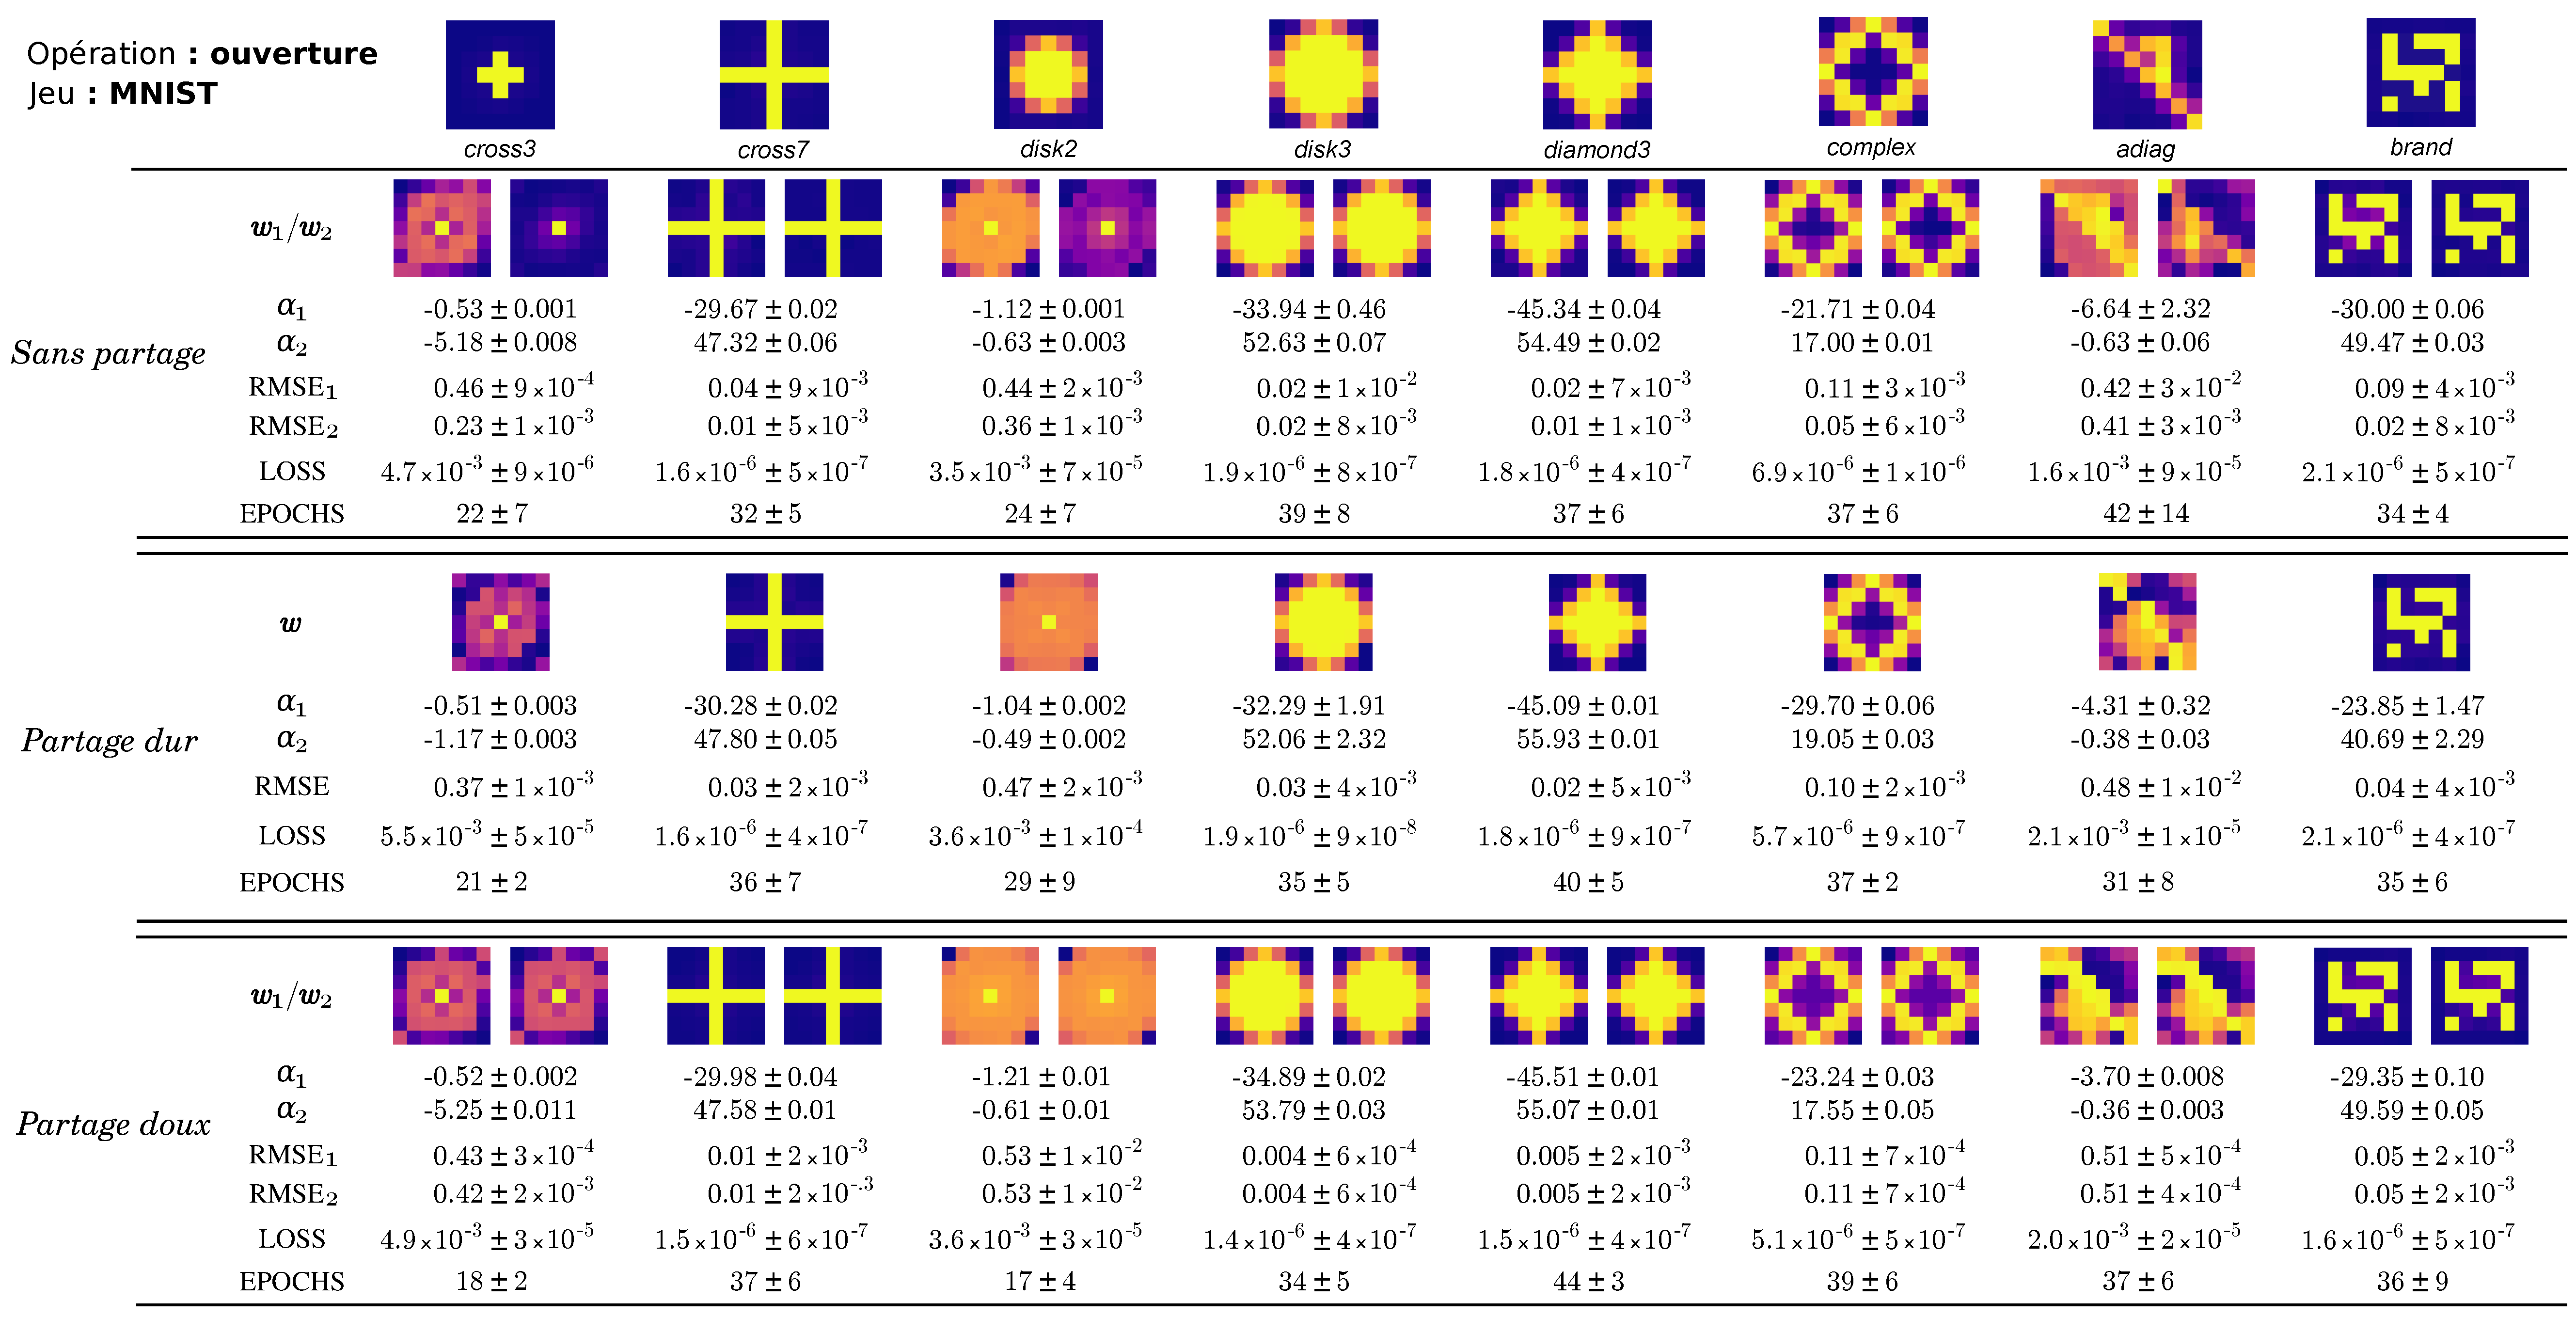
\includegraphics[width=1.00\linewidth]{parts/3-contributions/B-partage_de_poids/figures/h_opening_mnist.pdf}
    \vspace{-4.0mm}
    \caption{ \centering Comparaison des poids appris et des moyennes et écarts-types des métriques $\alpha$, \textit{RMSE}, \textit{loss} et nombre d'époques, et ce sur six runs, entre partage de poids dur, doux et sans partage, pour les huit fonctions structurantes cibles et l'opération d'\textbf{ouverture}.}
    \label{fig:MSEvsMSEpFSIM_opening}

    \bigskip

    \vspace{6.0mm}
    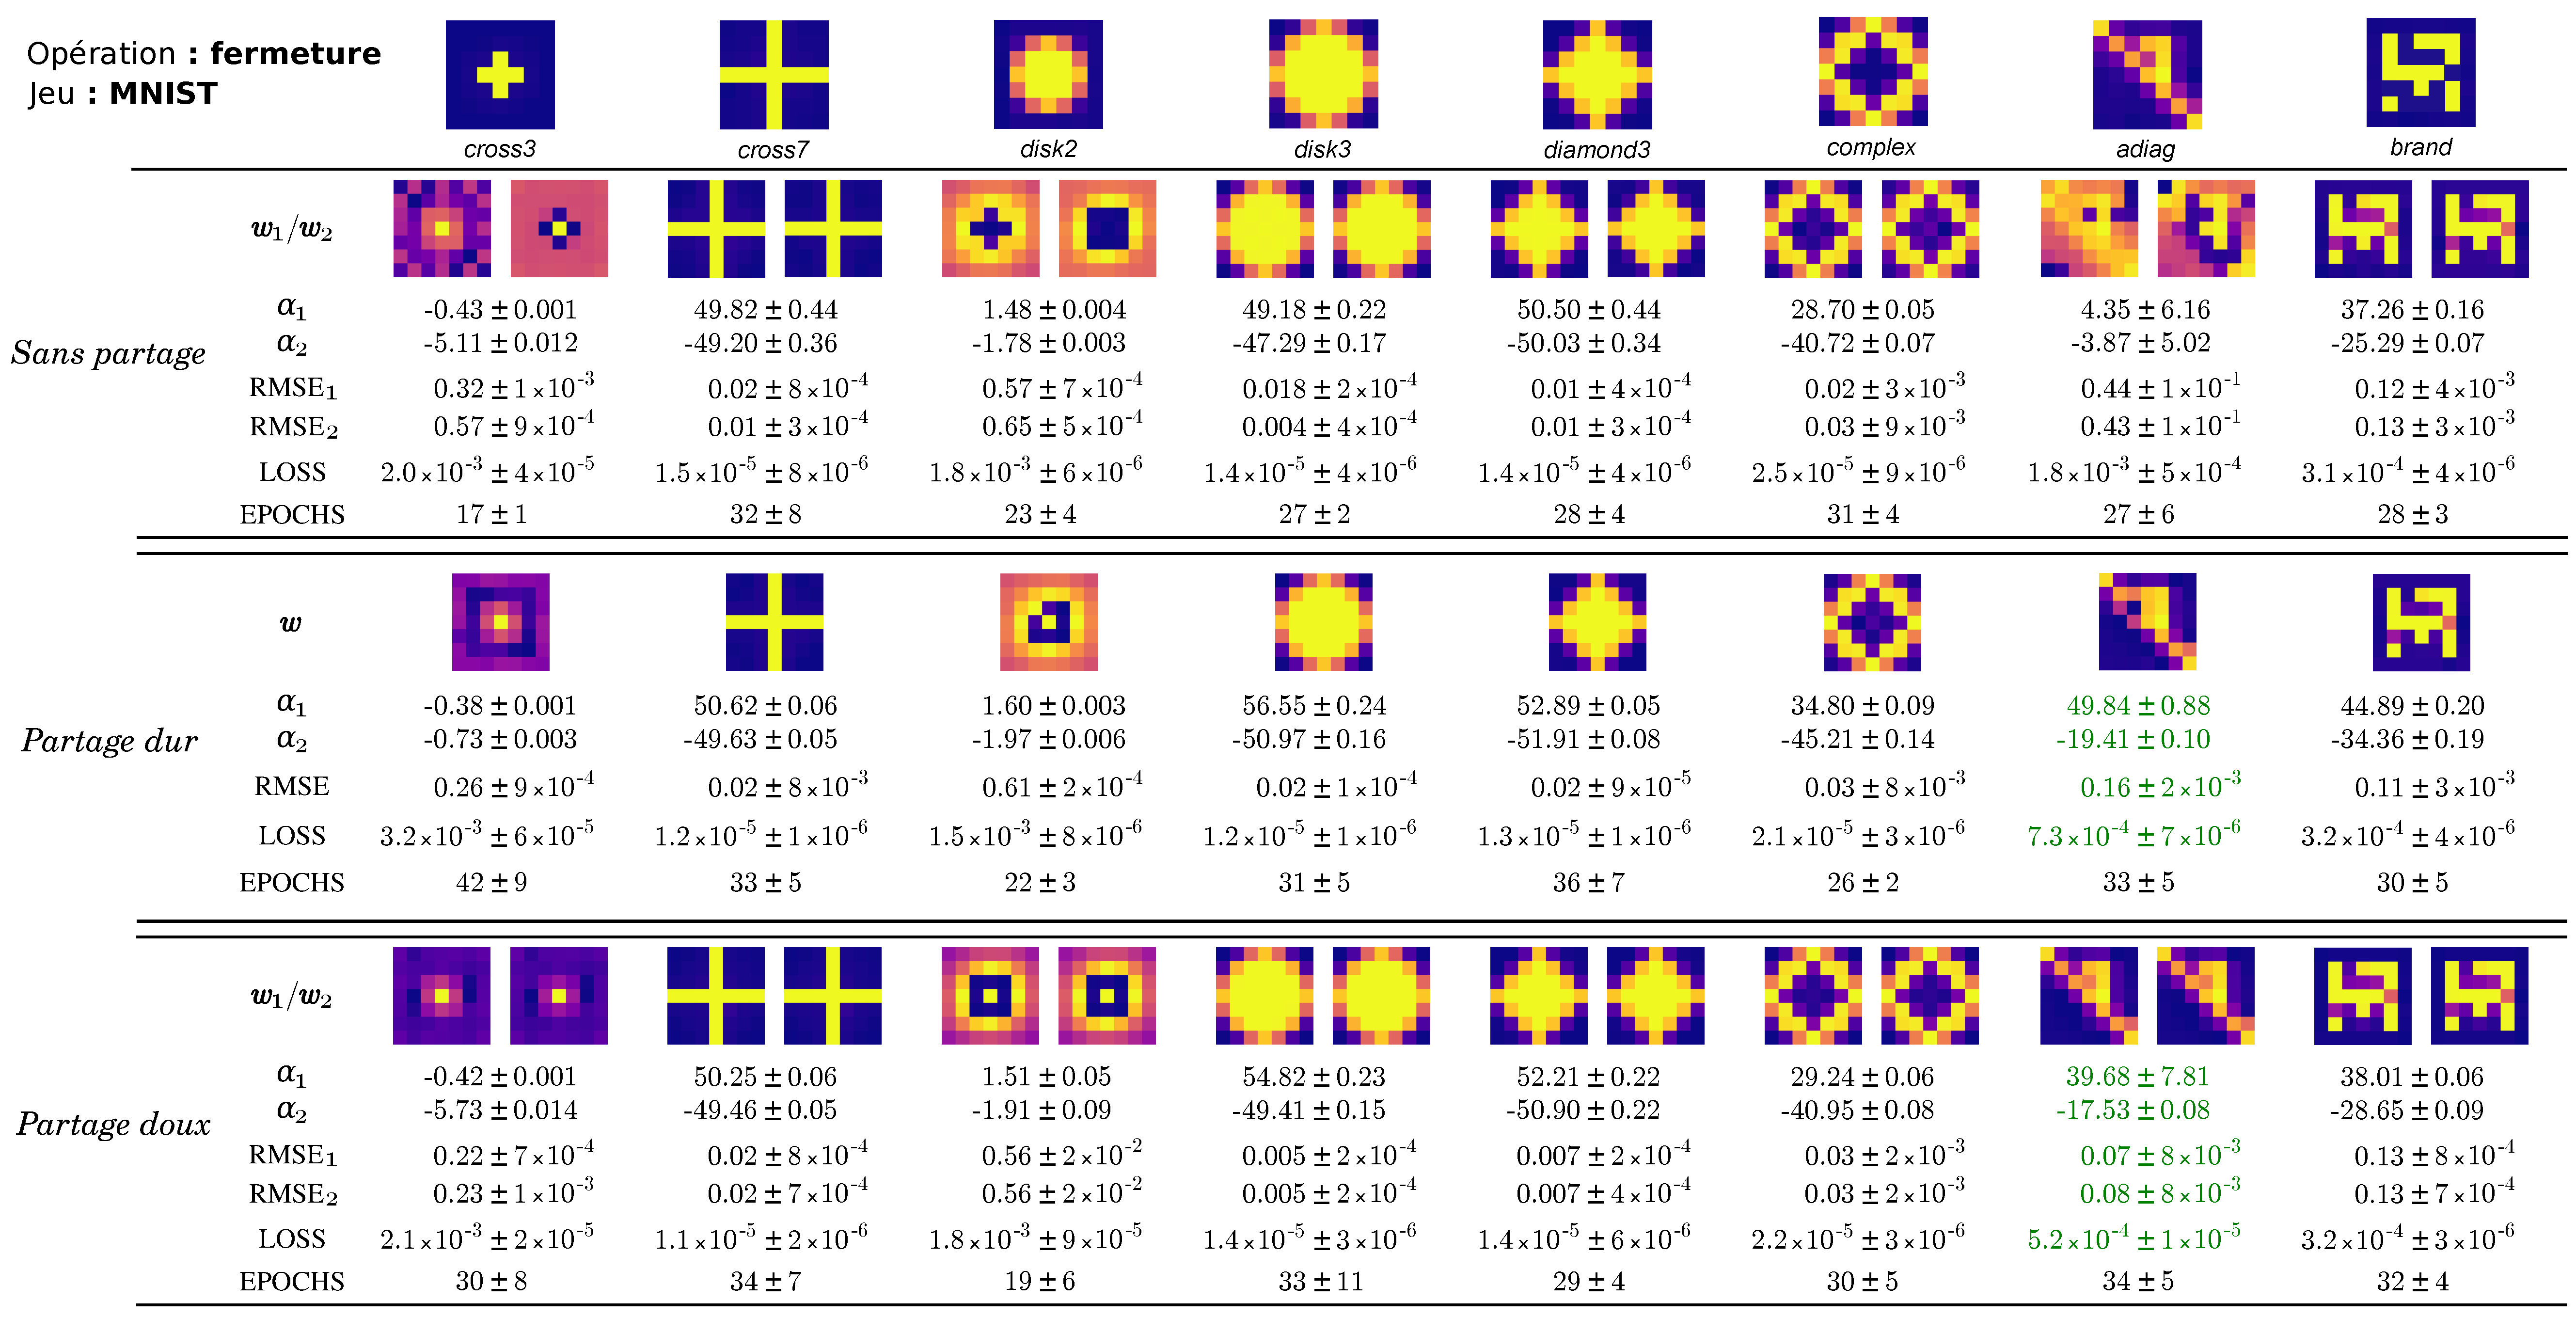
\includegraphics[width=1.00\linewidth]{parts/3-contributions/B-partage_de_poids/figures/h_closing_mnist.pdf}
    \vspace{-4.0mm}
    \caption{ \centering Comparaison des poids appris et des moyennes et écarts-types des métriques $\alpha$, \textit{RMSE}, \textit{loss} et nombre d'époques, et ce sur six runs, entre partage de poids dur, doux et sans partage, pour les huit fonctions structurantes cibles et l'opération de \textbf{fermeture}.}
    \label{fig:MSEvsMSEpFSIM_closing}
    
  \end{center}
\end{figure}


\newpage

%Les figures \ref{fig:MSEvsMSEpFSIM_opening} (ouverture) et \ref{fig:MSEvsMSEpFSIM_closing} (fermeture) montrent que les résultats de convergence des réseaux avec un partage des poids de leurs noyaux, que ce soit un partage dur ou doux, sont presque similaires aux résultats de ceux sans partage de poids. \\

%\vspace{-0.6mm}
Le réseau avec un partage de poids dur, comportant donc une couche duale, semble converger aussi bien voire un peu mieux que le réseau sans partage de poids. Dans les expériences où les réseaux sans partage de poids convergent initialement bien (\textit{cross7}, \textit{disk3}, \textit{diamond3}, \textit{complex} et \textit{brand}), ceux avec un partage de poids dur convergent au moins aussi bien, voire mieux dans certains cas (dans l'expérience avec la structure \textit{brand} et l'opération cible d'ouverture (fig. \ref{fig:MSEvsMSEpFSIM_opening}), il y a par exemple moins d'artéfacts sur le noyau de la couche duale que sur les noyaux du réseau sans partage). \\

\vspace{-3.0mm}
\noindent Dans les expériences où les réseaux sans partage de poids convergent, à l'inverse, initialement mal (forme des noyaux et valeurs des métriques trop mauvaises, comme \textit{cross3}, \textit{disk2} et \textit{adiag}), ceux avec un partage de poids dur convergent de la même manière, à l'exception de l'expérience avec la structure \textit{adiag} pour la fermeture (fig. \ref{fig:MSEvsMSEpFSIM_closing}), où le noyau de la couche converge ici vers la bonne forme cible, et où les métriques de performance du réseau présentent une perte \textit{loss} et une \textit{RMSE} bien plus faibles. \\

\vspace{-2.0mm}
Le réseau avec un partage doux, quant à lui, présente exactement les mêmes conclusions que le réseau avec un partage dur, bien que les formes des noyaux des réseaux et les métriques de performance soient légèrement différentes. Il présente des résultats similaires au réseau sans partage de poids. Comme pour le partage dur, seule l'expérience avec la structure \textit{adiag} pour l'opération de fermeture montre une bien meilleure convergence du réseau, avec une forme des noyaux proche de celle de la cible et de plutôt bons résultats au niveau des métriques de performance. \\

\vspace{-2.0mm}
En conclusion, ces deux méthodes de partage de poids des noyaux ne permettent pas forcément au réseau d'être plus efficace sur chaque expérience, mais résolvent tout de même le problème de convergence de \textit{adiag} pour la fermeture. De plus, elles donnent toutes deux des résultats similaires, bien que la forme des noyaux puisse être légèrement différente de l'un à l'autre sur certaines expériences. 
Les conclusions sont les mêmes avec la banque FashionMNIST, bien que les résultats soient assez différents. \\
%En conclusion, les réseaux implémentant ces deux méthodes de partage de poids peuvent être considérés comme équivalents aux réseaux sans partage, en terme d'efficacité et de précision. Ils ne sont donc pas forcément plus efficaces, mais résolvent tout de même le problème de convergence de \textit{adiag} pour la fermeture. De plus, les deux méthodes de partage de poids donnent des résultats similaires, bien que la forme des noyaux soient légèrement différents de l'un à l'autre sur certaines expériences. \\


%%%%%%%%%%%

%\vspace{1.6mm}
\noindent \textbf{Remarque :} \\

\vspace{-1.6mm}
\noindent Ici, on fait un partage de poids uniquement sur les noyaux. On aurait également pu partager inversement les $\alpha$ des deux couches, mais on considère qu'il s'agit là d'une bien trop forte hypothèse dans de nombreux contextes. En effet, pour des images cibles dont on ne connait pas l'ensemble des opérations duquel ces images résultent à partir d'images initiales, imposer au réseau bi-couches considéré de partir soit vers une opération de (pseudo-)ouverture soit vers une opération de (pseudo-)fermeture (car, dans un tel partage de poids, on imposerait une valeur opposée aux deux alphas du réseau) est une hypothèse déjà trop forte pour un tel système cible d'opérations inconnues, là où, au contraire, on peut se dire qu'il est plutôt plausible que les deux noyaux du réseau tendent à converger vers la même forme. Un tel partage inverse des $\alpha$ est cependant à considérer si l'on sait à l'avance que l'on veut soit un comportement d'ouverture soit de fermeture pour de tels réseaux à deux couches (partie suivante).

\newpage

% Partage de poids
\subsection{Contraintes sur les poids} %Partage de poids

\subsubsection{Contexte et motivations}
\vspace{0.2cm}
Les résultats précédents montrent qu'il reste encore quelques cas d'échecs de convergence pour les réseaux $\mathcal{S}$MorphNetTanh à deux couches morphologiques, avec les opérations cibles d'ouverture et de fermeture, et ce malgré l'ajout d'un partage doux des poids entre les noyaux $w$ des deux couches et l'ajout dans la \textit{loss} d'une contrainte $C_\text{awayOPP}$ entre les deux paramètres de contrôle $\alpha$ (ou $p$) associés. \\

\vspace{-1.4mm}
\noindent La modulation de l'initialisation des noyaux $w$ du réseau devient alors une solution potentielle à ces derniers échecs. ALors que les poids des noyaux sont originellement initialisés selon une loi normale centrée réduite afin de brasser les différents états de convergence possibles à partir d'initialisations aléatoires différentes sur plusieurs expériences, on peut finalement se dire que cette forme initiale des noyaux peut être fixée et définie de manière déterminée au préalable, selon des caractéristiques morphologiques générales à priori que l'on connait ou que l'on recherche sur ces noyaux. \\

\vspace{-1.4mm}
\noindent En l'occurence, on peut facilement s'imaginer que ce que l'on recherche ou favorise dans nos différents cas d'étude, c'est une forme de noyaux centrée sur son support et peu dispersée. On choisira alors une initialisation sous la forme d'une gaussienne 2D, allant de $0$ aux coins de l'image des noyaux à $1$ en son centre (voir figure \ref{fig:init_gauss} suivante). \\


%figure
\vspace{-1.0mm}
\begin{figure}[htp]
  \begin{center}
    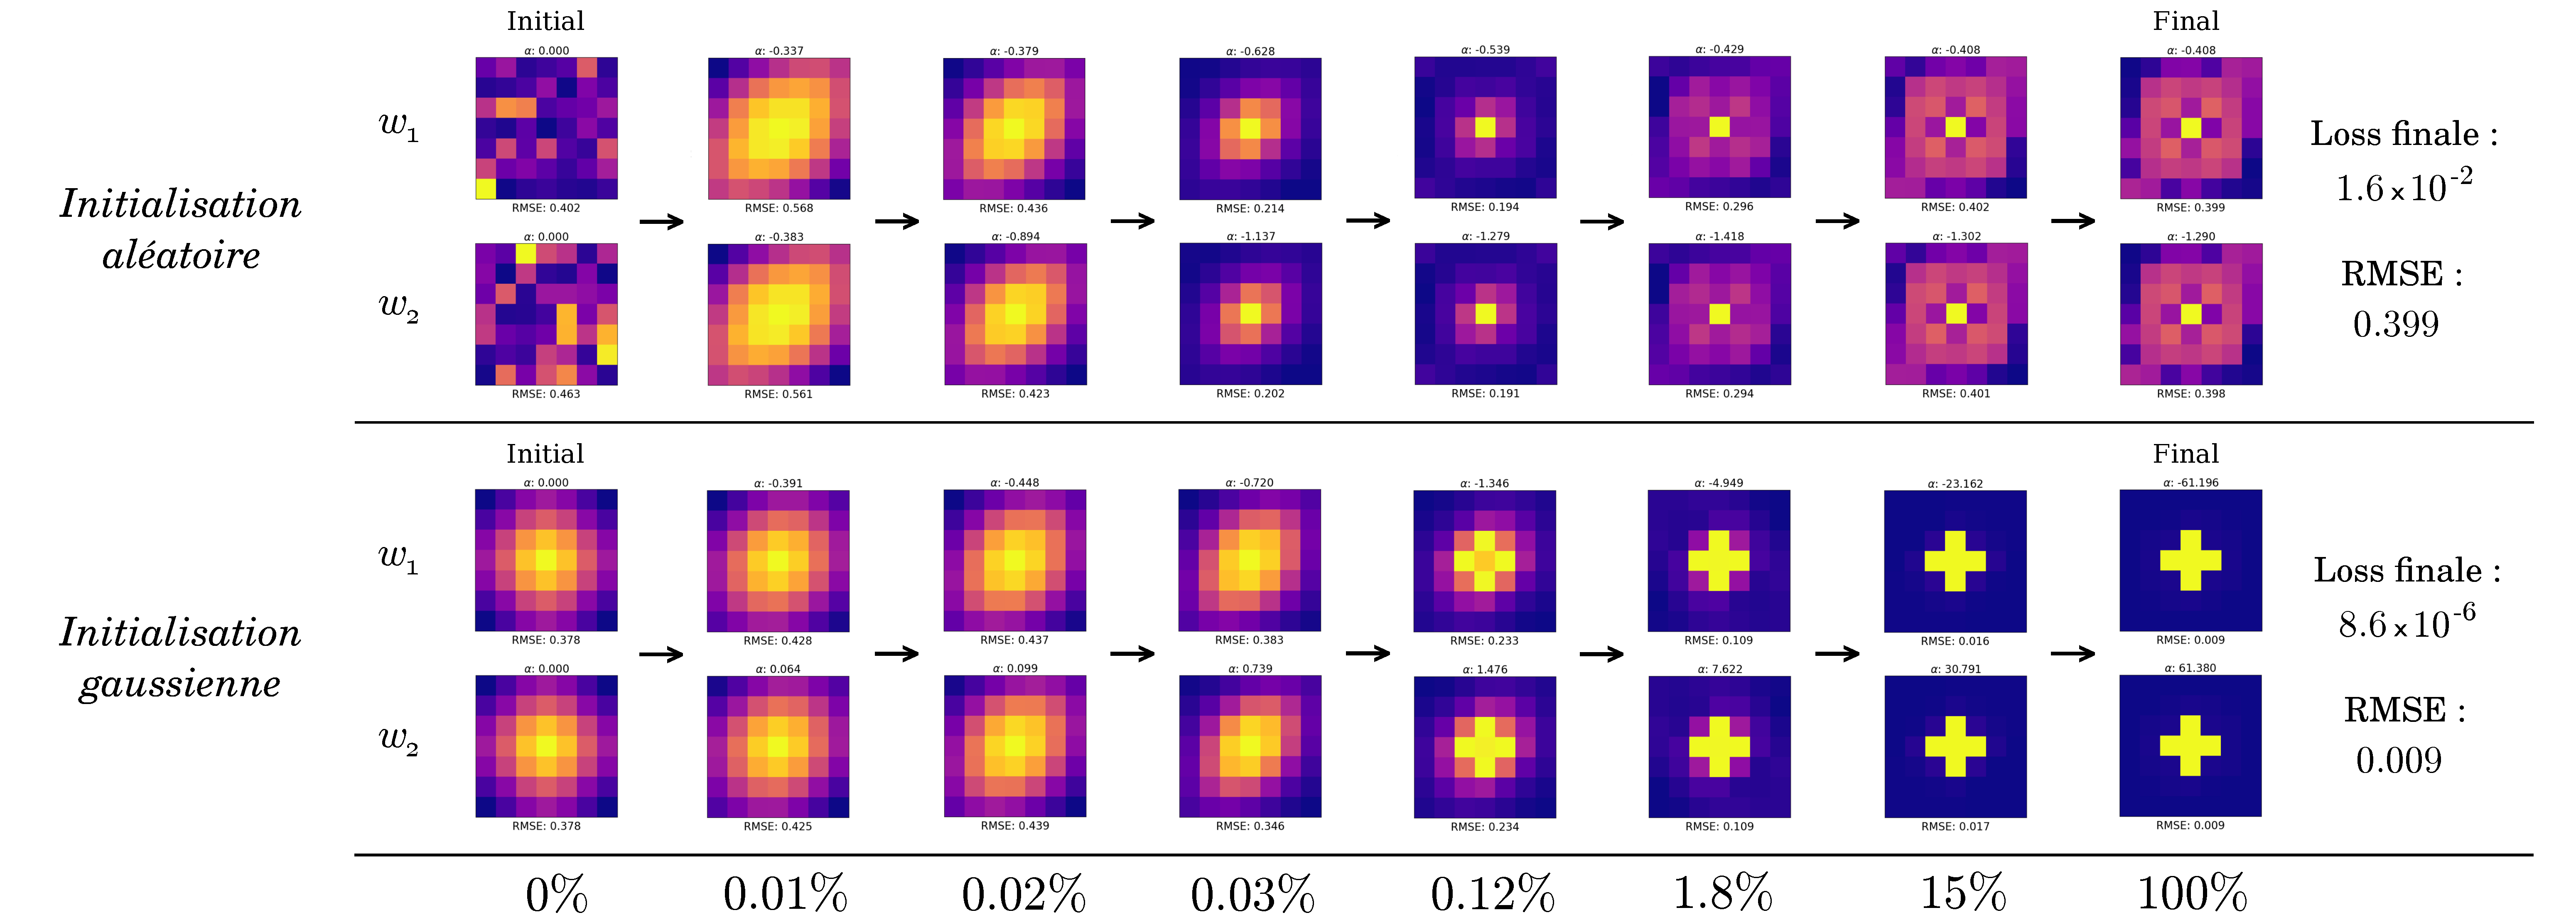
\includegraphics[width=1.00\linewidth]{parts/3-contributions/D-modulation_de_l_initialisation/figures/k_gauss.pdf}
    \vspace{-4.0mm}
    \caption{ \centering Évolution de la forme du noyau des deux couches du réseau et de sa \textit{RMSE} en fonction de la progression de l'entraînement (en \% avant l'état final), pour le \textit{cross3} et l'ouverture sur la banque MNIST, avec initialisation aléatoire et init. gaussienne.}
    \label{fig:init_gauss}
  \end{center}
\end{figure}


\vspace{-3.0mm}
\noindent L'exemple fig. \ref{fig:init_gauss}, obtenu sur six runs, montre bien ici l'efficacité de cette initialisation gaussienne des noyaux $w$ par rapport à l'aléatoire normale centrée réduite sur \textit{cross3} pour l'ouverture sur MNIST, avec des valeurs de \textit{RMSE} et de \textit{loss} bien plus faibles.

%\newpage

\subsubsection{Contraintes géométriques sur les noyaux $w$}
\vspace{0.2cm}
Le premier type de contraintes sur les poids des réseaux morphologiques est celui porté sur la géométrie des noyaux $w$ des couches de ces réseaux. 
Sont développées et étudiées dans cette sous-partie les différentes métriques de contraintes géométriques utilisées pendant le stage. On distingue ici cinq contraintes géométriques : l'erreur sur le centre de masse $C_\text{center}$ ; l'erreur sur la dispersion $C_\text{disp}$ ; l'erreur sur la symétrie $C_\text{sym}$ ; l'erreur sur la binarité $C_\text{binary}$ ; et l'erreur sur la norme $C_\text{norm}$. \\
%$\mathcal{S}$MorphNetTanh
\vspace{0.0mm}


%%%%%%%%%%%%%%%%%%%%%%%%%%%%%%%%%%%%%%%%%%%%%%%%%%%%%%%%%%%%%%%%%%%%%%%%%%%%%%%%%%%%%%%%%%%%%%%%%%%%%%%%%%%%%%
%%%%%%%%%%%%%%%%%%%%%%%%%%%%%%%%%%%%%%%%%%%%% 1e contrainte %%%%%%%%%%%%%%%%%%%%%%%%%%%%%%%%%%%%%%%%%%%%%%%%%%
%%%%%%%%%%%%%%%%%%%%%%%%%%%%%%%%%%%%%%%%%%%%%%%%%%%%%%%%%%%%%%%%%%%%%%%%%%%%%%%%%%%%%%%%%%%%%%%%%%%%%%%%%%%%%%

\noindent \textbf{a. Erreur sur le centre de masse}\\
\vspace{-0.6mm}

La première métrique de contrainte géométrique sur les noyaux $w$ des réseaux morphologiques est l'erreur sur le centre de masse, notée $C_\text{center}$. Soit $w: W \subseteq \mathbb{Z}^2 \rightarrow \mathbb{R}$ un noyau de couche. On prolonge $\mathbb{Z}^2$ dans $\mathbb{R}^2$, et on considère $\mathbb{R}^2$ comme un espace vectoriel muni de la norme euclidienne $\| \text{\raisebox{\mylen}{\tiny$\bullet$}} \|$. Le centre de masse $p_w \in \mathbb{R}^2$ de $w$ est défini par :

\vspace{-3.4mm}
\begin{equation}
    p_w = \frac{1}{\sum_{x \in W} w(x)} \sum_{x \in W} w(x) x
    \label{mass_center}
\end{equation}


\newpage

\vspace{3.6mm}
Soit $p_c \in \mathbb{R}^2$ le point << central >> visé, et soit $\zeta > 0$ (par défaut, $\zeta = 2$). L'erreur $C_\text{center}$ sur le centre de masse $p_w$ de $w$ par rapport à $p_c$ est définie par :

\vspace{2.6mm}
\begin{equation}
    C_\text{center}(w, p_c)_\zeta = \frac{ \left \| p_w - p_c \right \| ^\zeta }{ \sup_{p \in W} \left \| p - p_c \right \| ^\zeta }
    \label{erreur_center}
\end{equation}

\vspace{6.4mm}
Dans la pratique, on voudra faire tendre le centre de masse $p_w$ du noyau $w$ vers le centre de son support $W$ (de taille finie) dans $\mathbb{R}^2$. Dans ce cas : $p_c = \frac{1}{|W|} \sum_{x \in W} x$ . \\

%\vspace{-1.8mm}
\noindent Prenons par exemple l'expérience avec \textit{disk3} pour la fermeture sur FashionMNIST. La figure ci-après montre l'évolution de la convergence des deux noyaux du réseau, avec des checkpoints à différents stades durant l'entraînement, sans et avec cette contrainte $C_\text{center}$ dans la \textit{loss} (avec $\lambda = 0.01$). Dans les deux cas, le réseau possède le partage de poids doux tel que décrit précédemment. On obtient les mêmes résultats sur 6 runs. \\

%%% A chaque fois, faire deux comparaisons (schéma de l'évolution du filtre sur plusieurs périodes) : l'une sans la contrainte (prendre un truc qui converge mal), l'autre avec (prendre un truc qui converge bien) !

%figure
\vspace{0.6mm}
\begin{figure}[htp]
  \begin{center}
    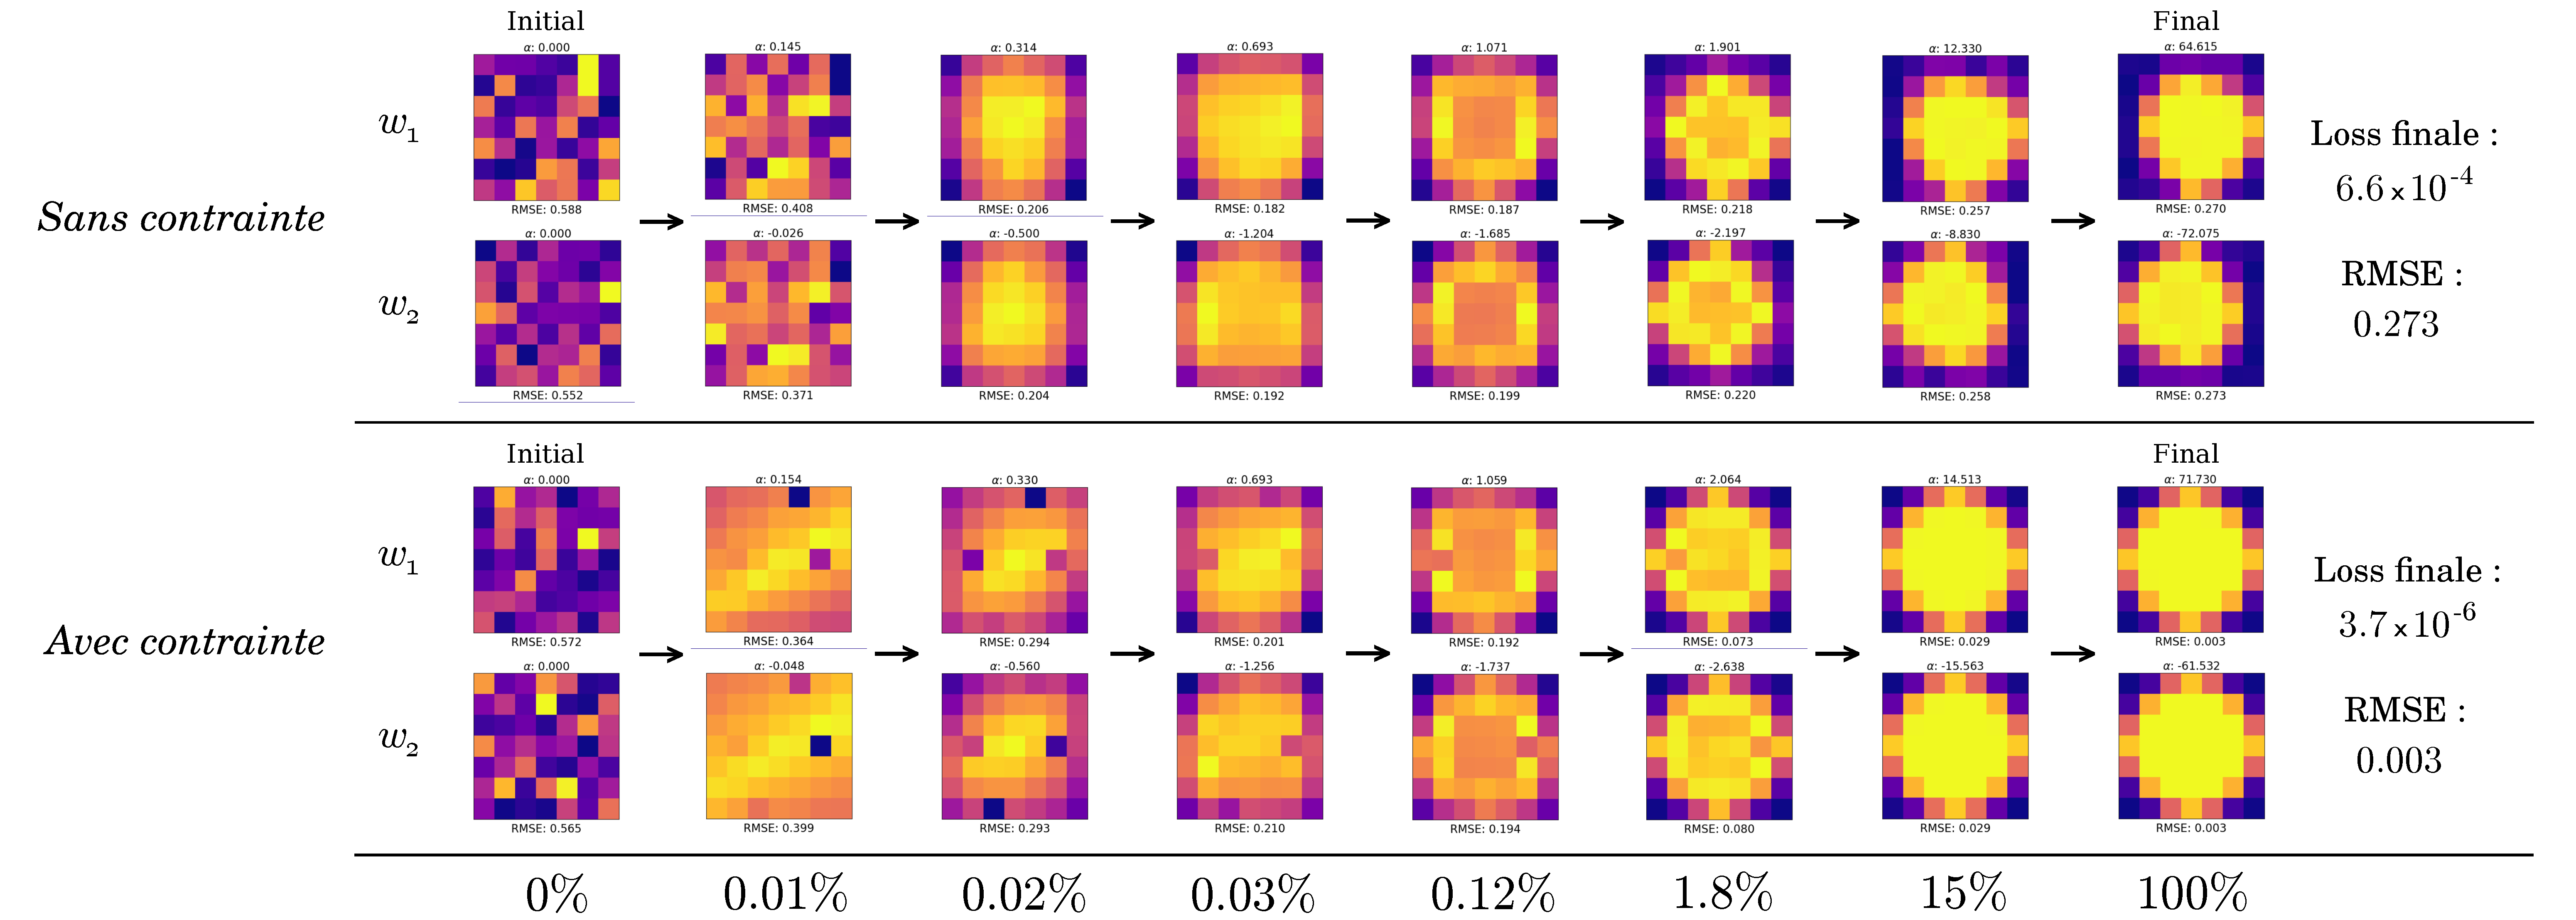
\includegraphics[width=1.00\linewidth]{parts/3-contributions/C-contraintes_geometriques/figures/k_center.pdf}
    \vspace{-4.0mm}
    \caption{ \centering Évolution de la forme du noyau des deux couches du réseau et de sa \textit{RMSE} en fonction de la progression de l'entraînement (en \% avant l'état final), pour le \textit{disk3} et la fermeture sur la banque FashionMNIST, avec et sans la contrainte $C_\text{center}$.}
    \label{fig:c_center}
  \end{center}
\end{figure}

\vspace{-0.2mm}
\noindent On voit sur la figure \ref{fig:c_center} que, sur cette expérience par exemple, avec la structure \textit{disk3} pour la fermeture et la banque FashionMNIST, cette métrique est très efficace pour avoir à la fois une \textit{RMSE} faible (la forme du noyau $w$ ressemble bien à la structure cible) et à la fois une \textit{loss} faible (le réseau a bien convergé).
Cependant, cette contrainte ne peut typiquement pas être appliquée dans le cas de fonctions structurantes cibles pour lesquelles le centre de masse est éloigné du centre du support, ou est inconnu. Comme expliqué dans les motivations, on ne pourra ainsi appliquer cette contrainte que dans des contextes particuliers où les informations nécessaires sont connues. \\


%%%%%%%%%%%%%%%%%%%%%%%%%%%%%%%%%%%%%%%%%%%%%%%%%%%%%%%%%%%%%%%%%%%%%%%%%%%%%%%%%%%%%%%%%%%%%%%%%%%%%%%%%%%%%%
%%%%%%%%%%%%%%%%%%%%%%%%%%%%%%%%%%%%%%%%%%%%% 2e contrainte %%%%%%%%%%%%%%%%%%%%%%%%%%%%%%%%%%%%%%%%%%%%%%%%%%
%%%%%%%%%%%%%%%%%%%%%%%%%%%%%%%%%%%%%%%%%%%%%%%%%%%%%%%%%%%%%%%%%%%%%%%%%%%%%%%%%%%%%%%%%%%%%%%%%%%%%%%%%%%%%%

\newpage

\noindent \textbf{b. Erreur sur la dispersion}\\

La deuxième métrique de contrainte géométrique sur les noyaux $w$ est l'erreur sur la dispersion, notée $C_\text{disp}$. Alors que l'erreur sur le centre de masse peut être associée à une moyenne (biais), l'erreur sur la dispersion peut être, quant à elle, associée à une variance. Soit $p_c \in \mathbb{R}^2$ le point de << concentration >> visé (en pratique, $p_c = p_w$), et soit $\zeta > 0$ (par défaut, $\zeta = 2$). L'erreur $C_\text{disp}$ sur la dispersion de $w$ par rapport à $p_c$ est définie par :

\vspace{-1.4mm}
\begin{equation}
    C_\text{disp}(w, p_c)_\zeta = \frac{ 1 }{ \sup_{p \in W} \left \| p - p_c \right \| ^\zeta } \frac{ 1 }{ \sum_{p \in W} w(p) } \sum_{p \in W} \left \| p - p_c \right \| ^\zeta w(p)
    \label{erreur_disp}
\end{equation}

\vspace{4.6mm}
%\noindent En pratique, on prendra : $p_c = p_w$ . \\

%\vspace{-2.0mm}
\noindent Prenons par exemple l'expérience avec \textit{disk2} pour la fermeture sur MNIST. La figure ci-après montre l'évolution de la convergence des deux noyaux du réseau, avec des checkpoints à différents stades durant l'entraînement, sans et avec cette contrainte $C_\text{disp}$ dans la \textit{loss} (avec $\lambda = 0.01$). Dans les deux cas, le réseau possède encore le partage de poids doux décrit précédemment. On obtient les mêmes résultats sur 6 runs. \\

%%% A chaque fois, faire deux comparaisons (schéma de l'évolution du filtre sur plusieurs périodes) : l'une sans la contrainte (prendre un truc qui converge mal), l'autre avec (prendre un truc qui converge bien) !

%figure
\vspace{0.4mm}
\begin{figure}[htp]
  \begin{center}
    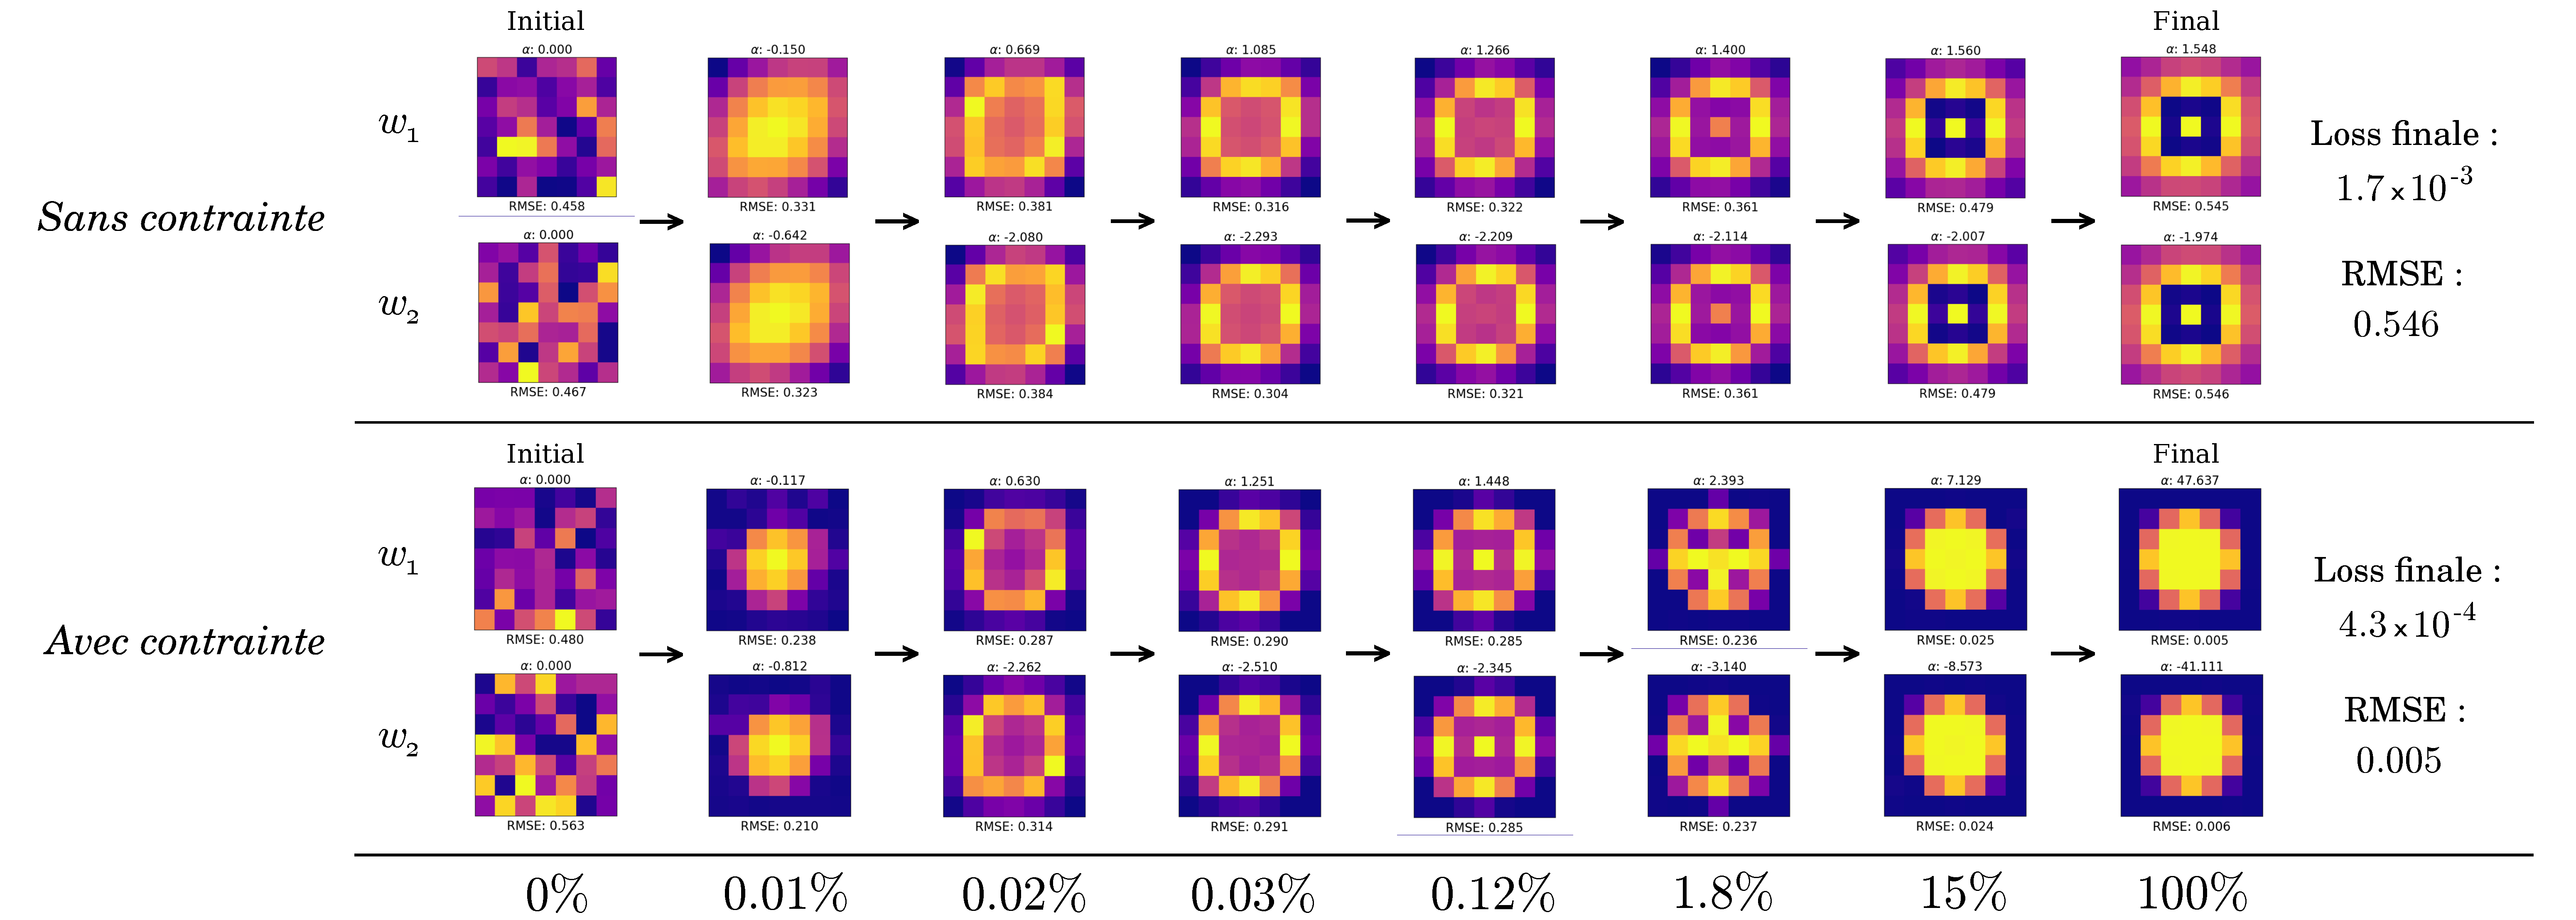
\includegraphics[width=1.00\linewidth]{parts/3-contributions/C-contraintes_geometriques/figures/k_disp.pdf}
    \vspace{-4.0mm}
    \caption{ \centering Évolution de la forme du noyau des deux couches du réseau et de sa \textit{RMSE} en fonction de la progression de l'entraînement (en \% avant l'état final), pour le \textit{disk2} et la fermeture sur la banque MNIST, avec et sans la contrainte $C_\text{disp}$.}
    \label{fig:c_disp}
  \end{center}
\end{figure}

\vspace{-1.6mm}
\noindent On voit sur la figure \ref{fig:c_disp} que, sur cette expérience par exemple, avec la structure \textit{disk2} pour la fermeture et la banque MNIST, cette métrique est très efficace pour avoir à la fois une \textit{RMSE} faible (la forme du noyau $w$ ressemble bien à la structure cible) et à la fois une \textit{loss} faible (le réseau a bien convergé).
Cependant encore, cette contrainte ne peut pas être appliquée dans le cas de fonctions structurantes cibles pour lesquelles les poids sont dispersés sur le support, ou dont la configuration est inconnue.


%%%%%%%%%%%%%%%%%%%%%%%%%%%%%%%%%%%%%%%%%%%%%%%%%%%%%%%%%%%%%%%%%%%%%%%%%%%%%%%%%%%%%%%%%%%%%%%%%%%%%%%%%%%%%%
%%%%%%%%%%%%%%%%%%%%%%%%%%%%%%%%%%%%%%%%%%%%% 3e contrainte %%%%%%%%%%%%%%%%%%%%%%%%%%%%%%%%%%%%%%%%%%%%%%%%%%
%%%%%%%%%%%%%%%%%%%%%%%%%%%%%%%%%%%%%%%%%%%%%%%%%%%%%%%%%%%%%%%%%%%%%%%%%%%%%%%%%%%%%%%%%%%%%%%%%%%%%%%%%%%%%%

\newpage

\noindent \textbf{c. Erreur sur la symétrie}\\

La troisième métrique de contrainte géométrique sur les noyaux $w$ des réseaux morphologiques est l'erreur sur la symétrie, notée $C_\text{sym}$. Soit $p_c \in \mathbb{R}^2$ le centre de symétrie visé (en pratique, $p_c = p_w$), et soit $\zeta > 0$ (par défaut, $\zeta = 2$). L'erreur $C_\text{sym}$ sur la symétrie centrale de $w$ par rapport au point $p_c$ est définie par :

\vspace{2.0mm}
\begin{equation}
    C_\text{sym}(w, p_c)_\zeta = 
    \frac{ 
    \sum_{p \in W} 
    \begin{cases}
        \hspace{1.4mm} \left | \hspace{0.7mm} w(p) - w( 2 p_c - p ) \hspace{0.7mm} \right | ^\zeta & \mbox{si} \hspace{3mm} 2 p_c - p \in W \\
        \hspace{1.4mm} \left ( w(p) - \inf_{q \in W} \{ w(q) \} \right ) ^\zeta & \mbox{sinon}
    \end{cases}
    }
    { |W| \left ( \sup_{p \in W} \{ w(p) \} - \inf_{p \in W} \{ w(p) \} \right ) ^\zeta }
    \label{erreur_sym}
\end{equation}

\vspace{4.5mm}
\noindent Prenons par exemple l'expérience avec \textit{diamond3} pour la fermeture sur la banque FashionMNIST. La figure ci-après montre l'évolution de la convergence des deux noyaux du réseau, avec des checkpoints à différents stades durant l'entraînement, sans et avec cette contrainte $C_\text{sym}$ dans la \textit{loss} (avec $\lambda = 0.01$). Dans les deux cas, le réseau possède toujours un partage de poids doux. On obtient les mêmes résultats sur 6 runs. \\

%%% A chaque fois, faire deux comparaisons (schéma de l'évolution du filtre sur plusieurs périodes) : l'une sans la contrainte (prendre un truc qui converge mal), l'autre avec (prendre un truc qui converge bien) !

%figure
\vspace{-0.2mm}
\begin{figure}[htp]
  \begin{center}
    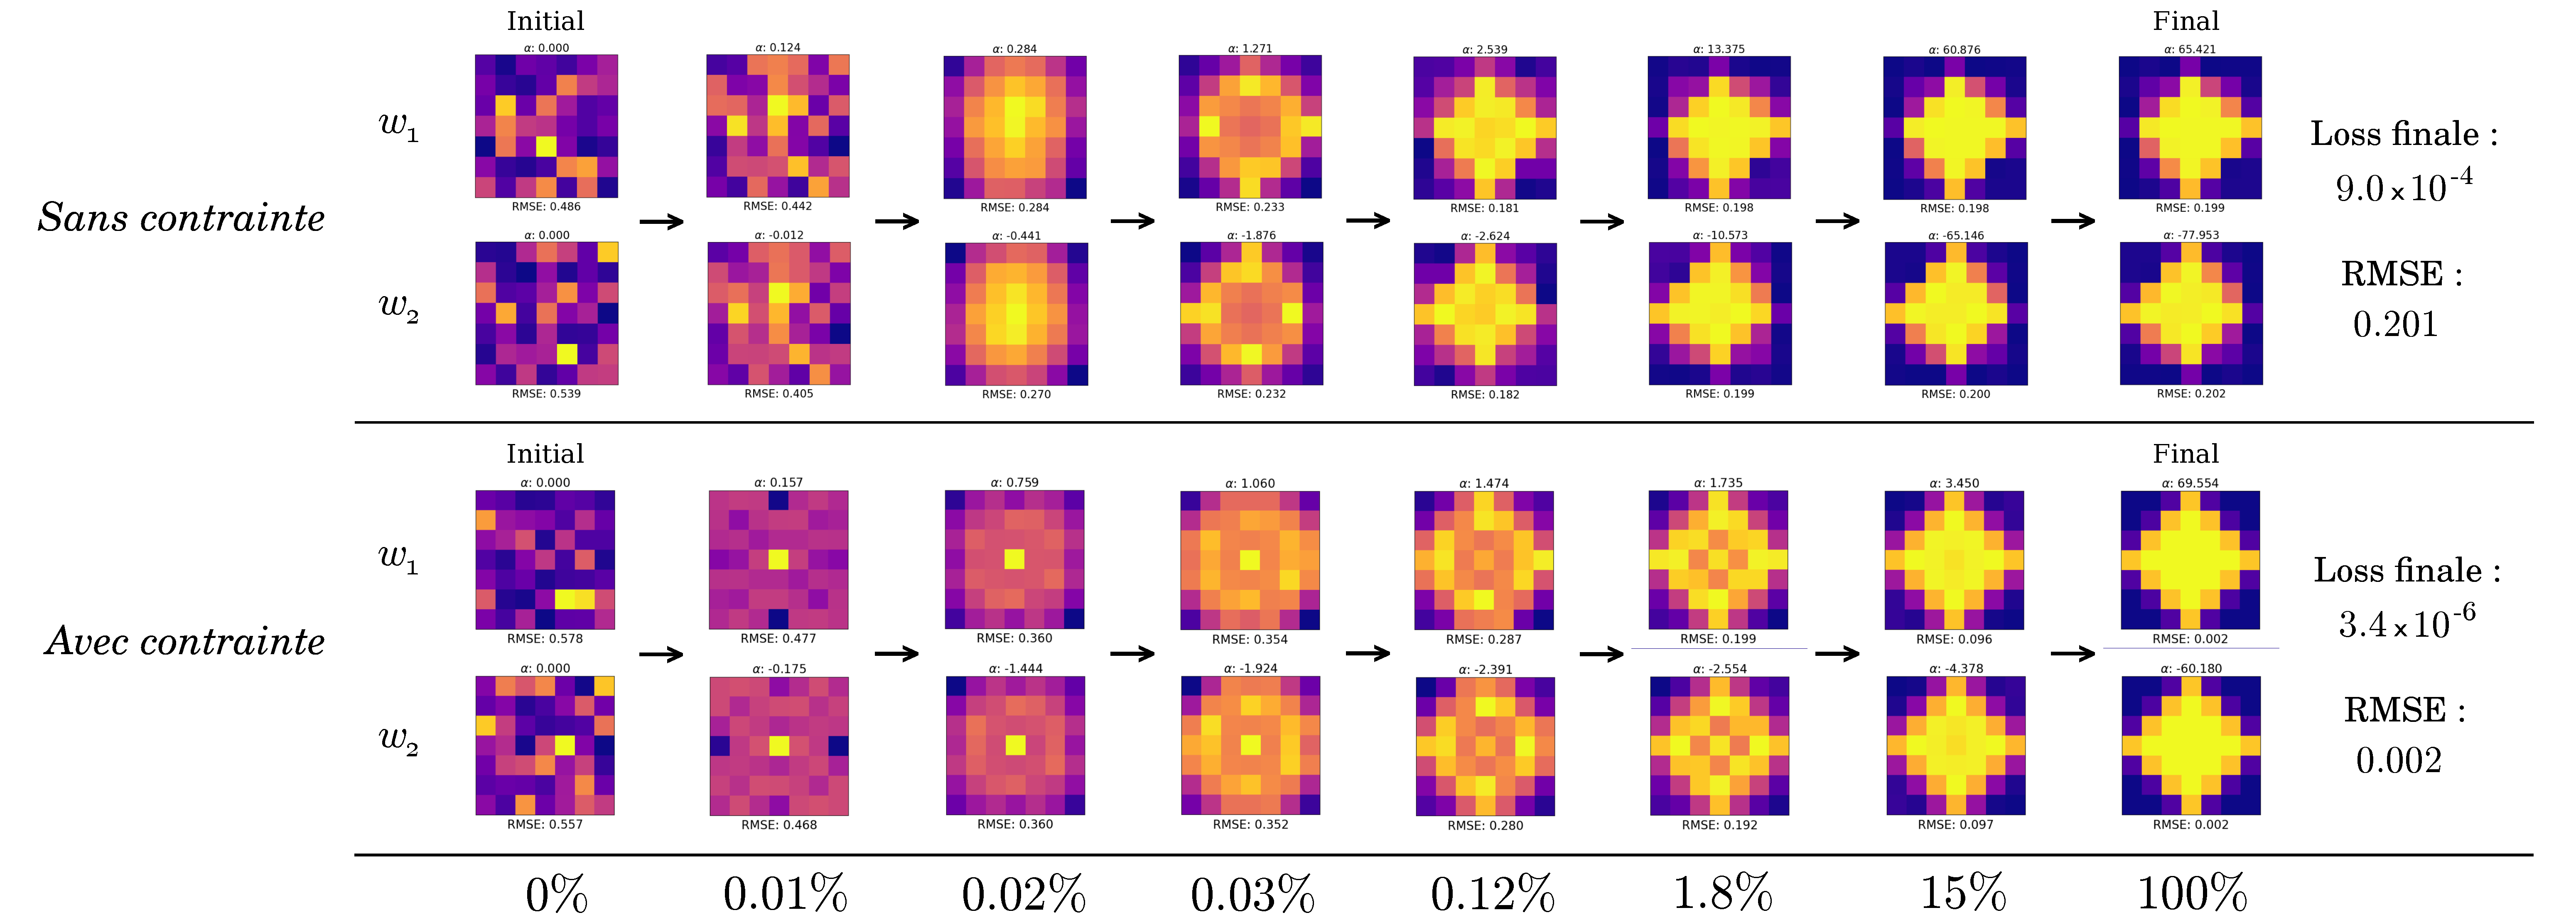
\includegraphics[width=1.00\linewidth]{parts/3-contributions/C-contraintes_geometriques/figures/k_sym.pdf}
    \vspace{-4.0mm}
    \caption{ \centering Évolution de la forme du noyau des deux couches du réseau et de sa \textit{RMSE} en fonction de la progression de l'entraînement (en \% avant l'état final), pour le \textit{diamond3} et la fermeture sur la banque FashionMNIST, avec et sans la contrainte $C_\text{sym}$.}
    \label{fig:c_sym}
  \end{center}
\end{figure}

\vspace{-2.4mm}
\noindent On voit sur la figure \ref{fig:c_sym} que, sur cette expérience par exemple, avec la structure cible symétrique \textit{diamond3} pour la fermeture et la banque FashionMNIST, cette métrique est efficace pour avoir à la fois une \textit{RMSE} faible (le noyau $w$ est proche de la structure cible) et à la fois une \textit{loss} faible (le réseau a bien convergé).
Encore une fois, cette contrainte ne peut cependant pas être appliquée dans le cas de fonctions structurantes cibles non symétriques (centralement), ou si le centre de symétrie est inconnu.


%%%%%%%%%%%%%%%%%%%%%%%%%%%%%%%%%%%%%%%%%%%%%%%%%%%%%%%%%%%%%%%%%%%%%%%%%%%%%%%%%%%%%%%%%%%%%%%%%%%%%%%%%%%%%%
%%%%%%%%%%%%%%%%%%%%%%%%%%%%%%%%%%%%%%%%%%%%% 4e contrainte %%%%%%%%%%%%%%%%%%%%%%%%%%%%%%%%%%%%%%%%%%%%%%%%%%
%%%%%%%%%%%%%%%%%%%%%%%%%%%%%%%%%%%%%%%%%%%%%%%%%%%%%%%%%%%%%%%%%%%%%%%%%%%%%%%%%%%%%%%%%%%%%%%%%%%%%%%%%%%%%%

\newpage

\noindent \textbf{d. Erreur sur la binarité}\\

La quatrième métrique de contrainte géométrique sur les noyaux $w$ des réseaux morphologiques est l'erreur sur la binarité, notée $C_\text{binary}$. Elle permet de faire converger les poids de $w$ vers deux bornes pré-définies, une inférieure $b_\text{inf} \in \mathbb{R}$ et une supérieure $b_\text{sup} \in \mathbb{R}$, avec $b_\text{sup} > b_\text{inf}$. En pratique, $b_\text{inf} = \inf_{p \in W} \{ w(p) \}$ et $b_\text{sup} = \sup_{p \in W} \{ w(p) \}$. Pour $\zeta > 0$ (par défaut, $\zeta = 2$), l'erreur $C_\text{binary}$ sur la binarité des poids de $w$ aux bornes $b_\text{inf}$ et $b_\text{sup}$ est définie par :

\vspace{-0.4mm}
\begin{equation}
    C_\text{binary}(w, (b_\text{inf}, b_\text{sup}))_\zeta = 
    \frac{1}{ |W| } 
    \sum_{p \in W} 
    \left |
    1 - \left | \frac{ 2 w(p) - b_\text{sup} - b_\text{inf} }{ b_\text{sup} - b_\text{inf} } \right | ^\zeta
    \right | ^\zeta
    \label{erreur_binary}
\end{equation}

\vspace{4.5mm}
\noindent Prenons par exemple l'expérience avec \textit{brand} pour la fermeture sur la banque MNIST. La figure ci-après montre l'évolution de la convergence des deux noyaux du réseau, avec des checkpoints à différents stades durant l'entraînement, sans et avec cette contrainte $C_\text{binary}$ dans la \textit{loss} (avec $\lambda = 0.0001$). Dans les deux cas, le réseau possède toujours un partage de poids doux. On obtient les mêmes résultats sur 6 runs. \\

%%% A chaque fois, faire deux comparaisons (schéma de l'évolution du filtre sur plusieurs périodes) : l'une sans la contrainte (prendre un truc qui converge mal), l'autre avec (prendre un truc qui converge bien) !

%figure
\vspace{-0.4mm}
\begin{figure}[htp]
  \begin{center}
    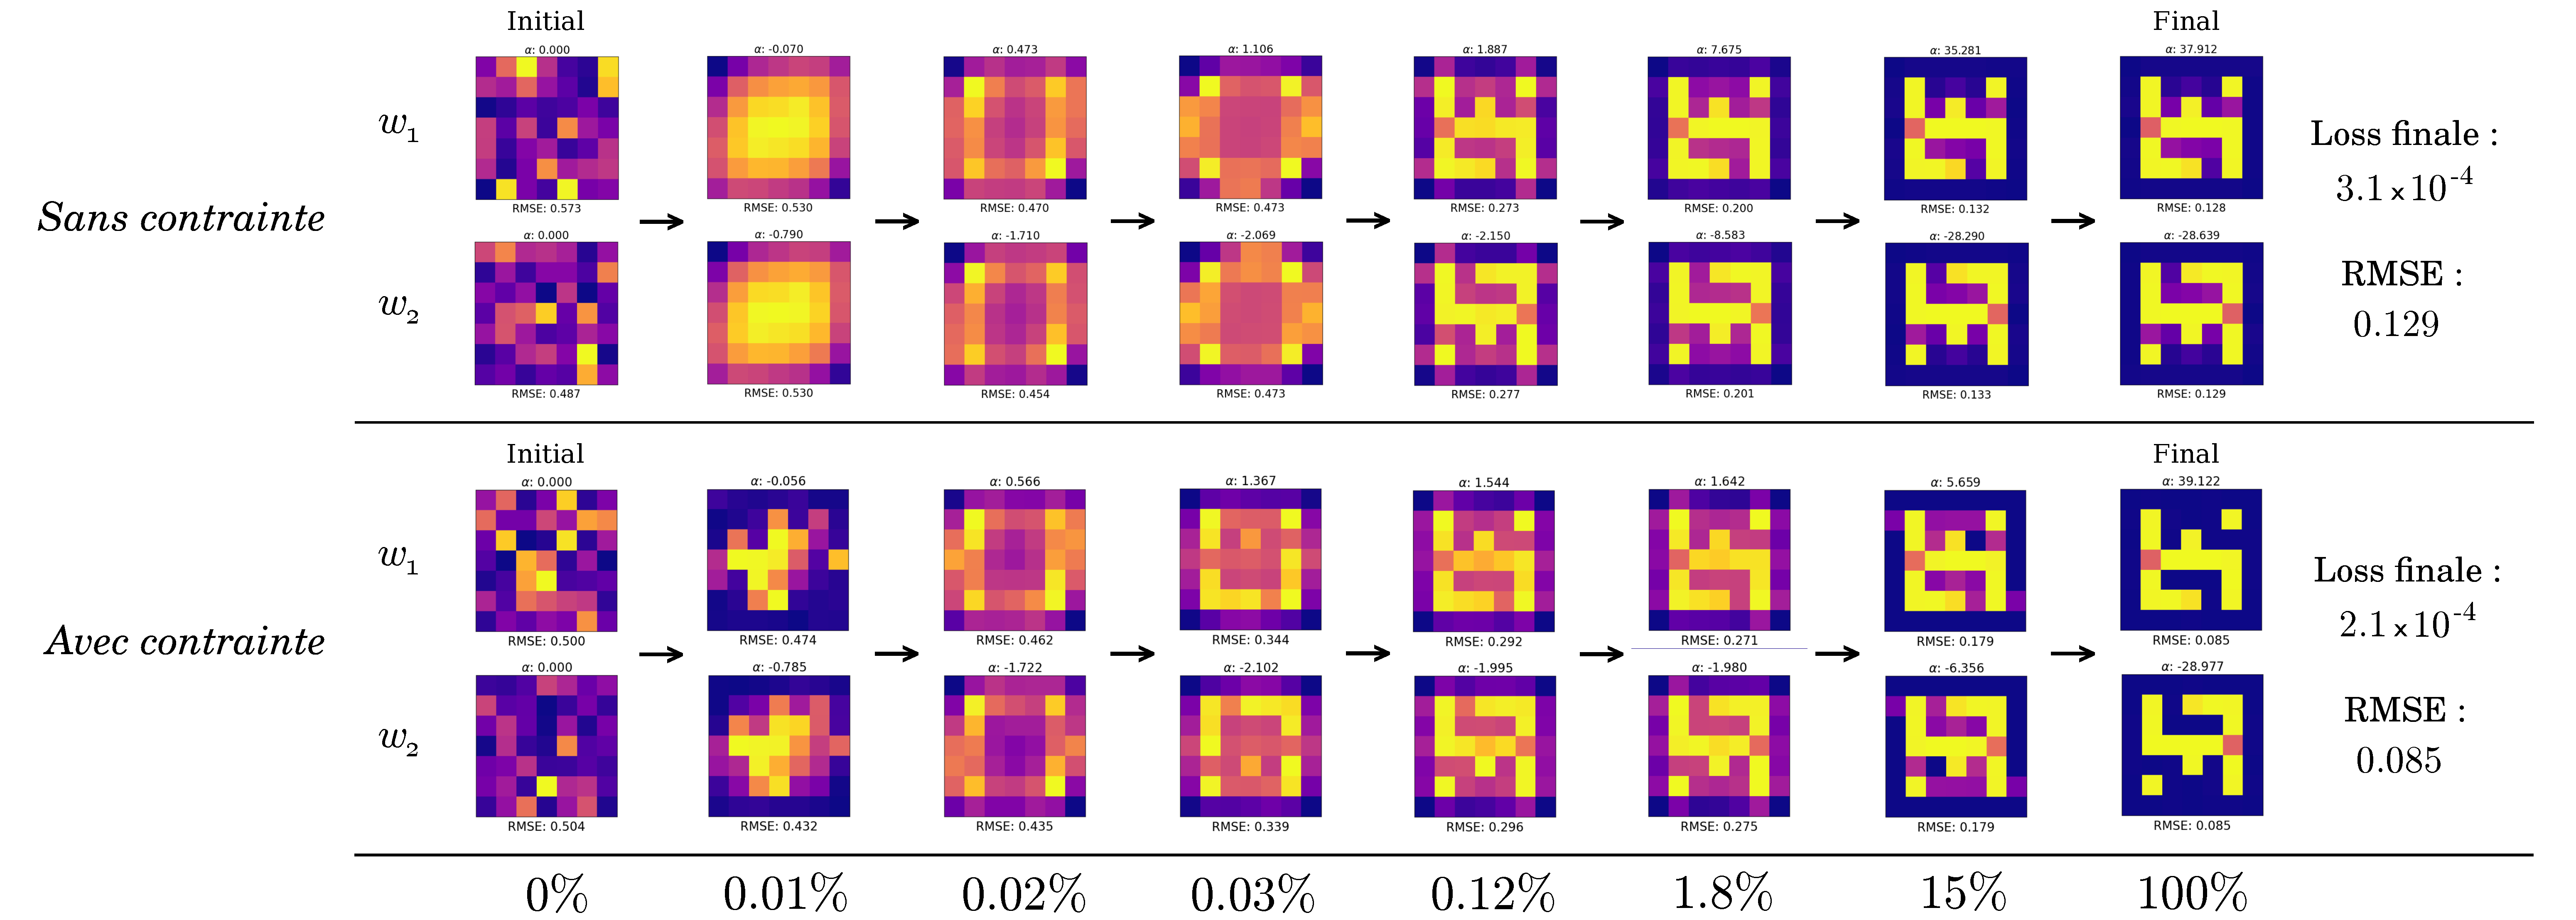
\includegraphics[width=1.00\linewidth]{parts/3-contributions/C-contraintes_geometriques/figures/k_binary.pdf}
    \vspace{-4.0mm}
    \caption{ \centering Évolution de la forme du noyau des deux couches du réseau et de sa \textit{RMSE} en fonction de la progression de l'entraînement (en \% avant l'état final), pour le \textit{brand} et la fermeture sur la banque MNIST, avec et sans la contrainte $C_\text{binary}$.}
    \label{fig:c_binary}
  \end{center}
\end{figure}

\vspace{-2.6mm}
\noindent On voit sur la figure \ref{fig:c_binary} que, sur cette expérience par exemple, avec la structure cible \textit{brand} pour la fermeture et la banque MNIST, cette métrique permet effectivement de mieux binariser les poids du noyau, et permet également une légère amélioration de la convergence du réseau, aussi bien sur la \textit{loss} que sur la \textit{RMSE}. Note : les images affichées sont les symétriques des noyaux $w$.
Précisons également que cette contrainte n'a pas de pertinence dans le cas de fonctions structurantes cibles non binaires.


%%%%%%%%%%%%%%%%%%%%%%%%%%%%%%%%%%%%%%%%%%%%%%%%%%%%%%%%%%%%%%%%%%%%%%%%%%%%%%%%%%%%%%%%%%%%%%%%%%%%%%%%%%%%%%
%%%%%%%%%%%%%%%%%%%%%%%%%%%%%%%%%%%%%%%%%%%%% 4e contrainte %%%%%%%%%%%%%%%%%%%%%%%%%%%%%%%%%%%%%%%%%%%%%%%%%%
%%%%%%%%%%%%%%%%%%%%%%%%%%%%%%%%%%%%%%%%%%%%%%%%%%%%%%%%%%%%%%%%%%%%%%%%%%%%%%%%%%%%%%%%%%%%%%%%%%%%%%%%%%%%%%

\newpage

\noindent \textbf{e. Erreur sur la norme}\\

La dernière métrique de contrainte géométrique sur les noyaux $w$ est l'erreur sur leur norme, notée $C_\text{norm}$. Elle permet à la norme du noyau de converger vers une valeur cible prédéfinie $l_c \in \mathbb{R}_+$. Par défaut, $l_c = 0$. L'erreur $C_\text{norm}$ sur la norme $n$, avec $n > 0$ (par défaut, $n = 1$), du noyau $w$ est définie, avec $\zeta > 0$ (par défaut, $\zeta = 2$), par :

%\vspace{-0.0mm}
\begin{equation}
    C_\text{norm}(w, l_c)_{n,\zeta} = 
    \frac
    { \left | 
    \left ( \sum_{p \in W} \left | w(p) \right | ^n \right ) ^{1/n} - l_c
    \right | ^\zeta }
    { |W| ^ {\zeta/n} \left ( \sup_{p \in W} \{ w(p) \} - \inf_{p \in W} \{ w(p) \} \right ) ^\zeta } 
    \label{erreur_norm}
\end{equation}

\vspace{4.5mm}
Par défaut, $n = 1$, car la norme \textit{1} est le meilleur approximateur convexe de la norme $0$ (on s'intéresse à la norme $0$ pour calculer la taille de l'<< objet >> du support). \\
%, i.e. le nombre de pixels de valeur strictement supérieure à 0). \\

\vspace{-2.6mm}
\noindent Prenons l'expérience avec \textit{complex} pour la fermeture sur la banque FashionMNIST. La figure ci-après montre l'évolution de la convergence des deux noyaux du réseau durant l'entraînement, sans et avec la contrainte $C_\text{norm}$ dans la \textit{loss} (avec $\lambda = 0.001$). Le réseau a toujours un partage de poids doux. On obtient ces résultats sur 6 runs. \\

%%% A chaque fois, faire deux comparaisons (schéma de l'évolution du filtre sur plusieurs périodes) : l'une sans la contrainte (prendre un truc qui converge mal), l'autre avec (prendre un truc qui converge bien) !

%figure
\vspace{-0.8mm}
\begin{figure}[htp]
  \begin{center}
    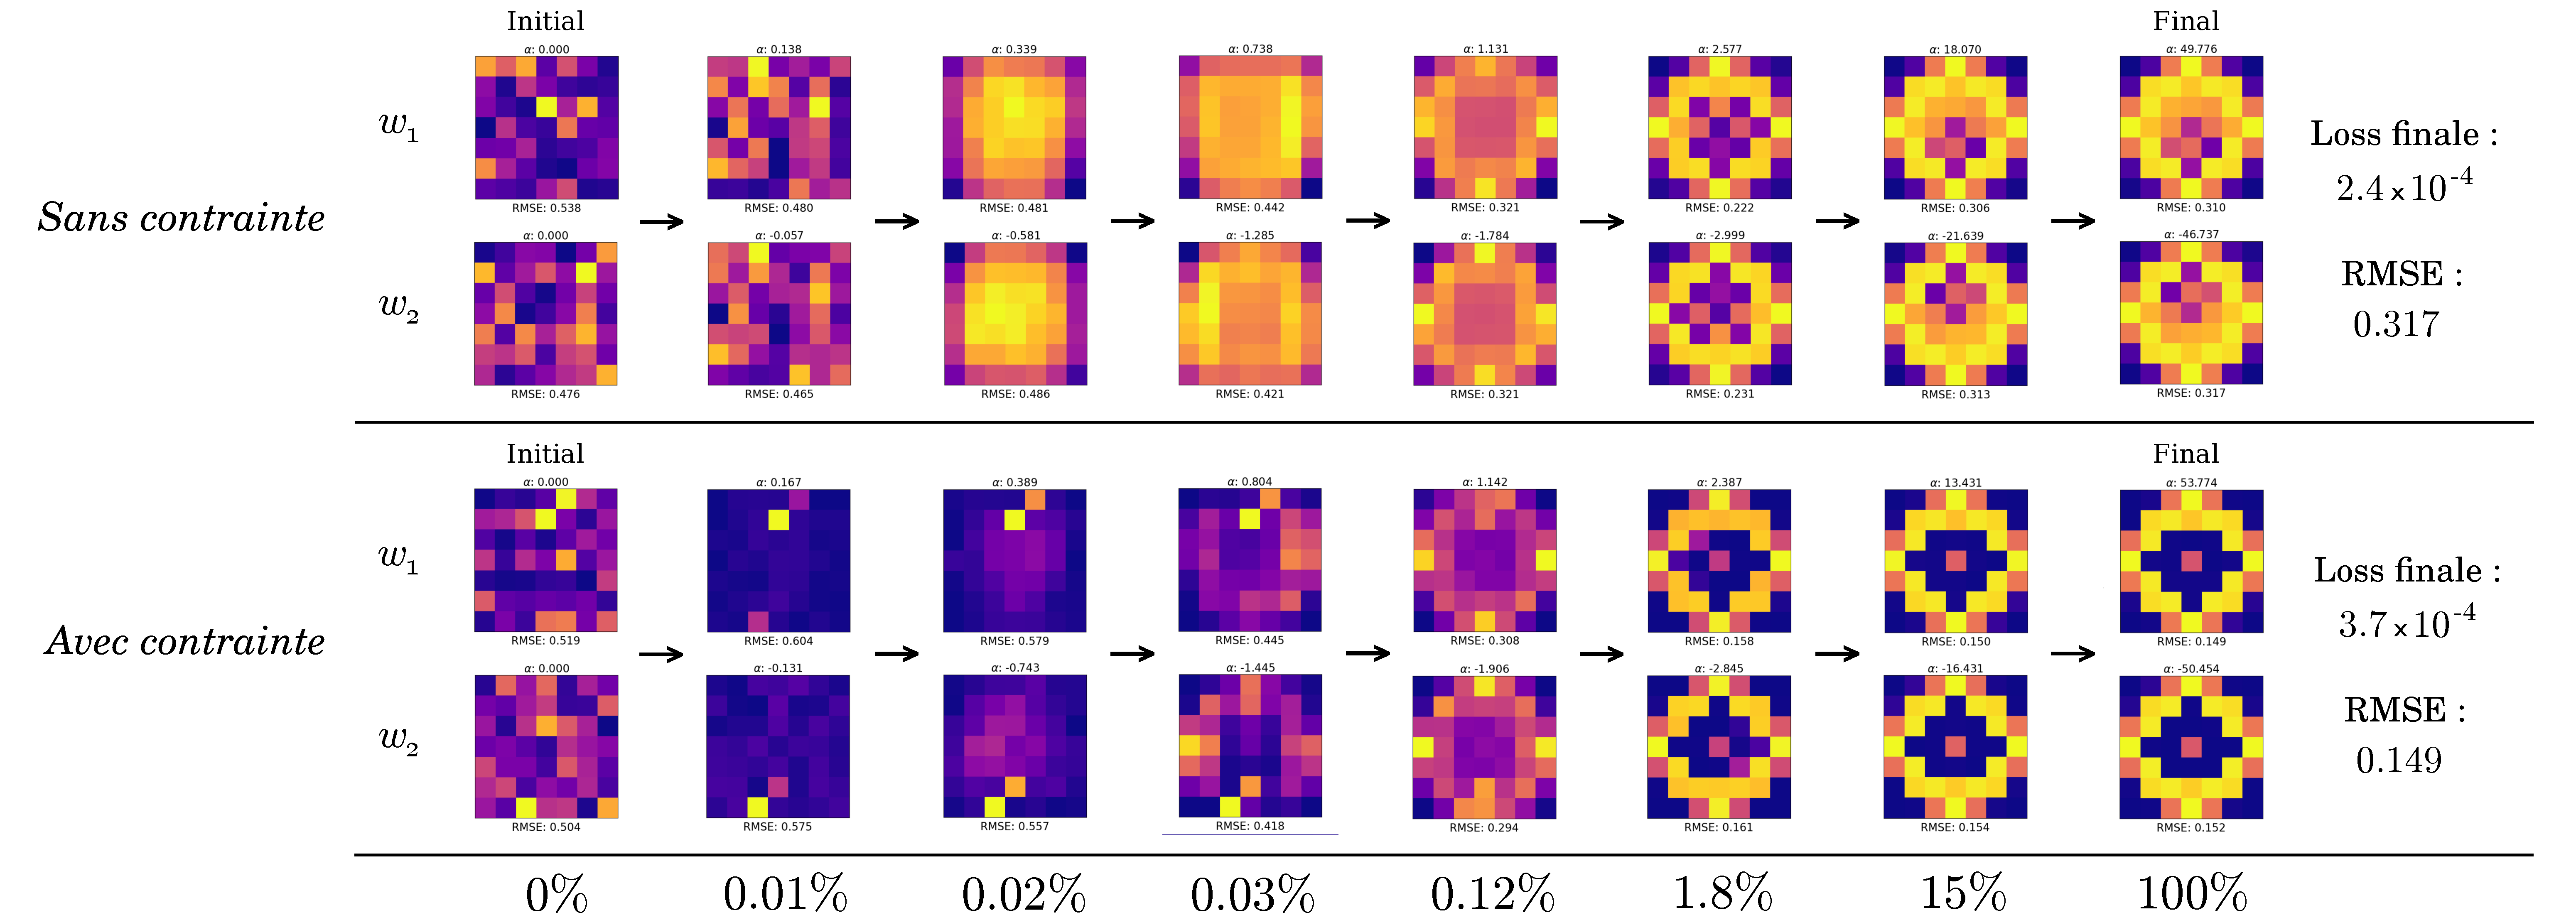
\includegraphics[width=1.00\linewidth]{parts/3-contributions/C-contraintes_geometriques/figures/k_norm.pdf}
    \vspace{-4.0mm}
    \caption{ \centering Évolution de la forme du noyau des deux couches du réseau et de sa \textit{RMSE} en fonction de la progression de l'entraînement (en \% avant l'état final), pour le \textit{complex} et la fermeture sur la banque FashionMNIST, avec et sans la contrainte $C_\text{norm}$.}
    \label{fig:c_norm}
  \end{center}
\end{figure}

\vspace{-3.0mm}
\noindent Cette contrainte permet de réduire le nombre de pixels nuisibles et d'artéfacts sur $w$ si l'hyperparamètre $\lambda$ est bien ajusté dans la \textit{loss}. Les résultats de la figure \ref{fig:c_norm} avec cette contrainte (où $l_c = 0$ et $\lambda = 0.001$) sont meilleurs en terme de \textit{RMSE}, mais un peu moins bons en terme de \textit{loss} par rapport à ceux sans $C_\text{norm}$.
Cette contrainte étant utilisée en particulier pour minimiser le nombre de pixels apparents dans $w$, elle peut donc être utilisée dans tout contexte si on veut avoir un objet minimal dans $w$ sur $W$.


\newpage

\noindent \textbf{Remarque pour l'ensemble des contraintes sur $w$ :} \\

\vspace{-1.0mm}
\noindent Dans les cas pratiques, on utilisera, pour ces cinq métriques de contraintes étudiées, le noyau $w$ \textit{normalisé}, écrit $\mathfrak{N}(w)$ (formule \ref{normalized}). Cela permet en particulier de distinguer l'<< objet >> (dont les valeurs sur $\mathfrak{N}(w)$ sont près de $1$) du << fond >> (dont les valeurs sur $\mathfrak{N}(w)$ sont près de $0$) sur le support $W$. De plus, si on est avec les réseaux $\mathcal{S}$MorphNet (classique, sans tangente hyperbolique Tanh) ou $\mathcal{L}$MorphNet, et si le paramètre $\alpha/p$ associé au noyau $w$ est négatif, alors on prend la négation $-w$ au lieu de $w$.

%\newpage

\subsubsection{Contraintes sur les paramètres de contrôle $\alpha$}
\vspace{0.2cm}
Le second type de contraintes sur les poids des réseaux est celui sur les paramètres de contrôle $\alpha$ des couches morphologiques (ou $p$ pour $\mathcal{L}$Morph et $p$Conv). On définit ici deux contraintes sur ces paramètres : l’erreur sur l'éloignement individuelle des $\alpha$ de $0$, notée $C_\text{away}$, et l’erreur sur l'éloignement opposé des $\alpha$, notée $C_\text{awayOPP}$. La première métrique évalue les paramètres $\alpha$ de manière indépendante, là où la seconde évalue deux paramètres de contrôle de deux couches, $\alpha_1$ et $\alpha_2$, en tant que couple. ELles permettent toutes deux de s'éloigner des cas de pseudo-opération. \\



\noindent \textbf{a. Erreur sur l'éloignement}\\

La première métrique de contrainte sur les paramètres de contrôle $\alpha$ (ou $p$ selon le type de réseau) est l'erreur sur leur éloignement individuelle de $0$, notée $C_\text{away}$. Elle permet de contraindre la fonction de perte \textit{loss} en la forçant de manière douce à faire éloigner de $0$ le poids $\alpha$ d'une couche morphologique, loin dans les positifs ou loin dans les négatifs selon la direction de convergence du réseau lors de l'entraînement, jusqu'à atteindre une valeur minimale objectif de $|\alpha|$, notée $\alpha_\text{min}$. \\

\vspace{-1.0mm}
\noindent Avec une valeur de $\alpha_\text{min} > 0$ fixée (par défaut, $\alpha_\text{min} = 80$), l'erreur $C_\text{away}$ sur l'éloignement du paramètre $\alpha$ d'une couche morphologique est définie, avec $\zeta > 0$ (par défaut, $\zeta = 2$), par :

\vspace{-1.0mm}
\begin{equation}
    C_\text{away}(\alpha, \alpha_\text{min})_\zeta = 
    \begin{cases}
        \hspace{1.0mm} \left | 
        \frac{ | \alpha |^\zeta - \alpha_\text{min} ^\zeta }{ \alpha_\text{min} ^\zeta } 
        \right | ^\zeta & \mbox{si} \hspace{3.0mm} | \alpha | < \alpha_\text{min} \\
        \hspace{2.0mm} 0 & \mbox{sinon}
    \end{cases}
    \label{erreur_away}
\end{equation}



\vspace{5.0mm}
\noindent Dans cette contrainte à nouveau, le paramètre $\zeta$ joue le rôle de régulateur de la fonction $x \mapsto |x|^\zeta$ en permettant d'adoucir la courbure de cette dernière, en particulier au voisinage de $0$, et de la rendre dérivable.
La métrique $C_\text{away}$ est ainsi continue et dérivable partout pour $\zeta > 1$. En particulier donc en $\alpha = 0$, ainsi qu'en $|\alpha| = \alpha_\text{min}$, là où la dérivée de la fonction est nulle pour $\zeta > 1$, et donc où la condition dans la définition de $C_\text{away}$ selon la valeur de $|\alpha|$ n'empêche pas la dérivabilité de cette fonction.


\newpage

%\noindent 
Prenons par exemple l’expérience avec \textit{complex} pour l'ouverture sur la banque d'images MNIST. La figure ci-après montre l’évolution de la convergence des deux noyaux $w_1$ et $w_2$ du réseau $\mathcal{S}$MorphNetTanh durant l’entraînement, d'abord sans puis avec la contrainte $C_\text{away}$ dans la fonction de perte \textit{loss} (avec $\lambda$ = 0.01).
Comme précédemment, le réseau a toujours un partage de poids doux entre les noyaux de ses deux couches morphologiques. On obtient les résultats suivants sur 6 runs. \\


%figure
\vspace{1.0mm}
\begin{figure}[htp]
  \begin{center}
    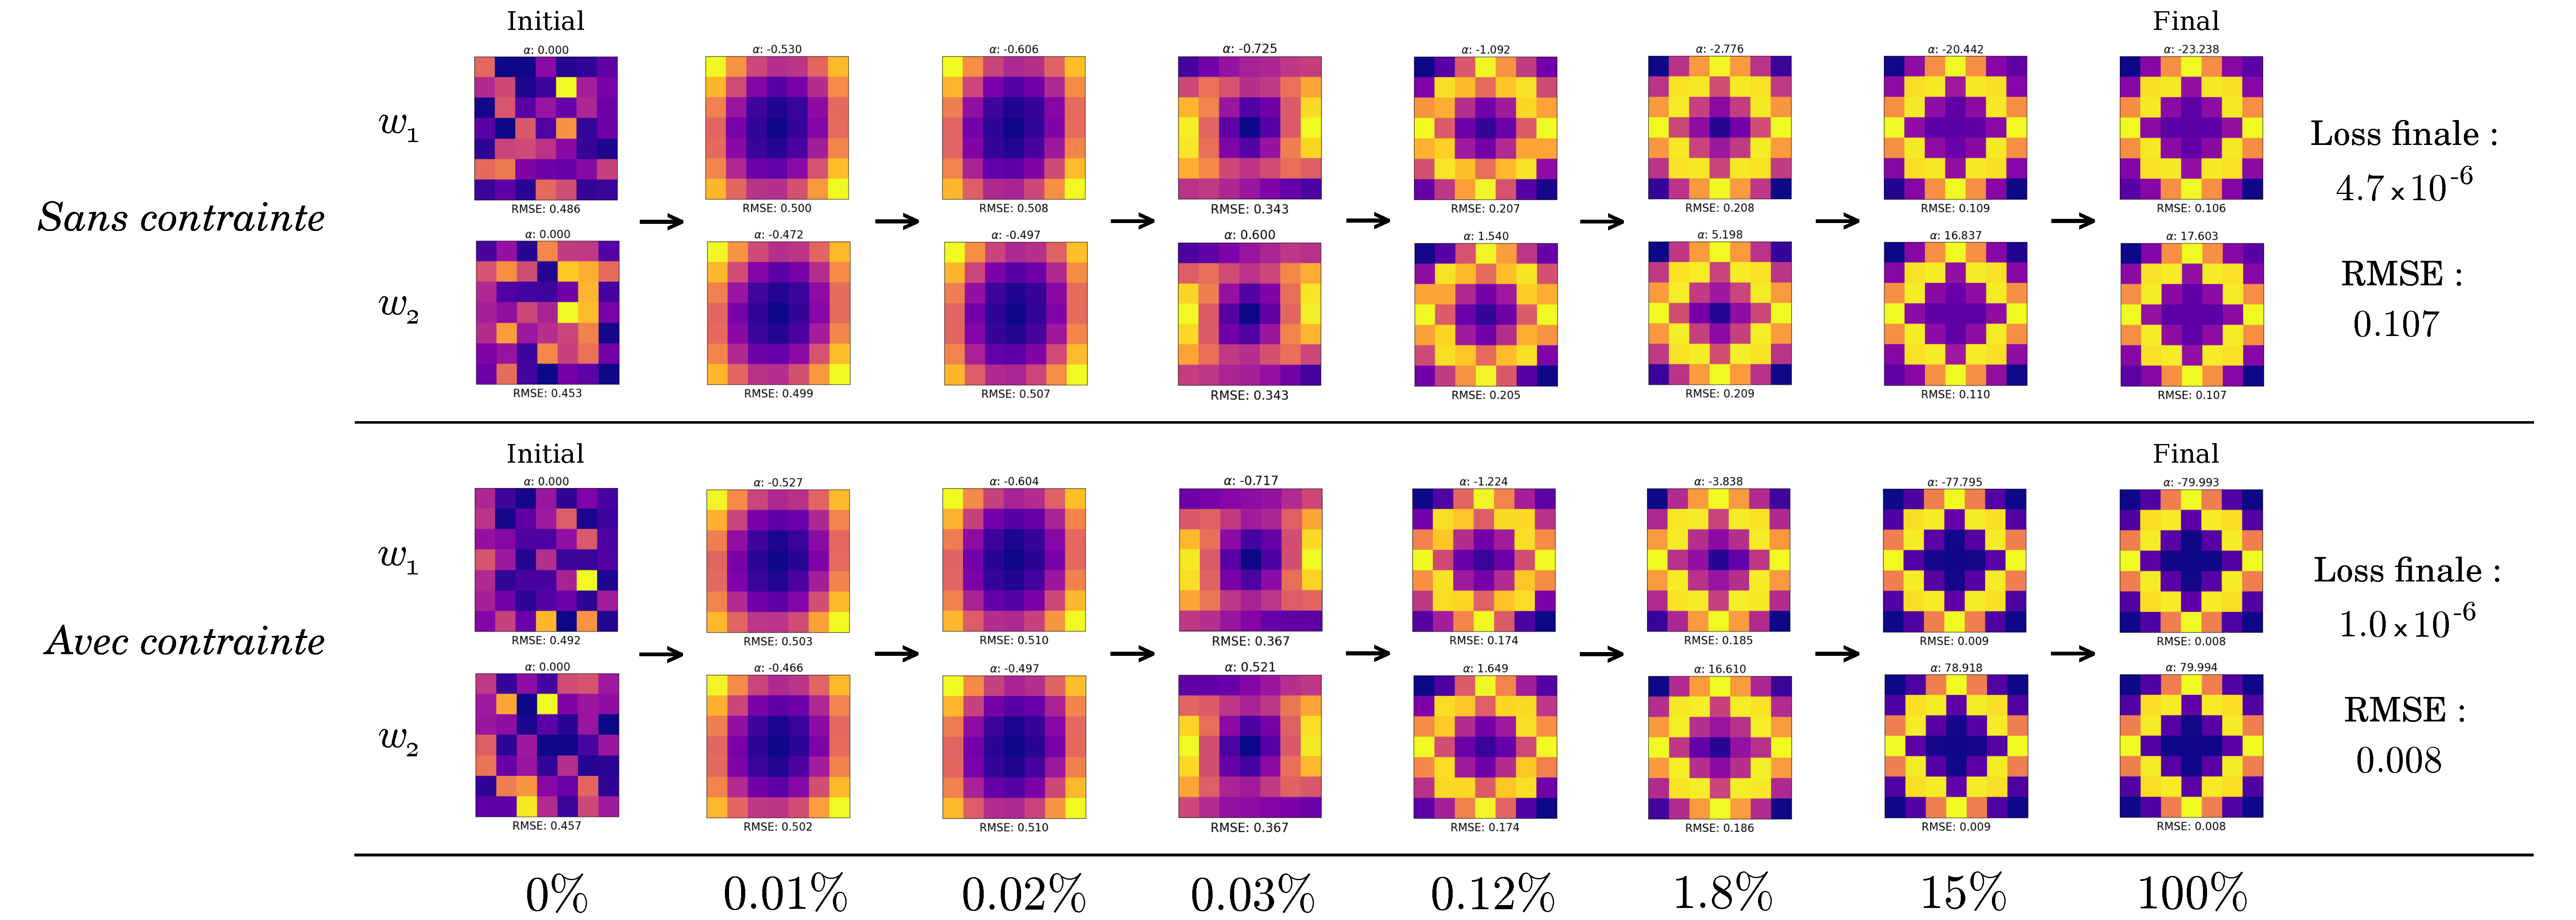
\includegraphics[width=1.00\linewidth]{parts/3-contributions/C-contraintes_geometriques/figures/k_away.pdf}
    \vspace{-4.0mm}
    \caption{ \centering Évolution de la forme du noyau des deux couches du réseau et de sa \textit{RMSE} en fonction de la progression de l'entraînement (en \% avant l'état final), pour le \textit{complex} et l'ouverture sur la banque MNIST, avec et sans la contrainte $C_\text{away}$.}
    \label{fig:c_away}
  \end{center}
\end{figure}


\vspace{-1.6mm}
\noindent À partir de ces résultats, on remarque que cette contrainte permet bien sur cet exemple d'éloigner les deux $\alpha$ de $0$, en les amenant dans ce cas près de $80$ en valeur absolue. On remarque également qu'elle permet ici d'améliorer automatiquement la forme des deux noyaux $w$ du réseau, en les rapprochant davantage de la structure cible (les artéfacts violets au centre et aux bords des noyaux sont réduits), avec une valeur de \textit{RMSE} bien plus faible, et cela simplement grâce à cet éloignement des $\alpha$. La valeur de la \textit{loss} est également plus faible, donc les prédictions sont meilleures grâce à cette contrainte. \\

\vspace{-0.2mm}
Cette contrainte semble efficace lorsque les noyaux $w$ convergent initialement, sans contrainte, vers une forme proche de celle de la fonction structurante cible, et que les paramètres de contrôle $\alpha$ associés sont encore relativement proches de $0$ mais bien du signe espéré et opposé pour les opérations cibles d'ouverture et de fermeture.
Cependant, après différentes expériences réalisées, cette métrique ne semble fonctionner que moyennement pour les expériences qui sont originellement des échecs sans cette contrainte, et pour lesquelles les paramètres $\alpha$ des deux couches du réseau ont le même signe. C'est le cas par exemple de l'expérience avec \textit{adiag} pour l'ouverture et la banque MNIST, pour laquelle $C_\text{away}$ ne permet pas l'éloignement des $\alpha$.


%%% A chaque fois, faire deux comparaisons (schéma de l'évolution du filtre sur plusieurs périodes) : l'une sans la contrainte (prendre un truc qui converge mal), l'autre avec (prendre un truc qui converge bien) !


\newpage

\noindent \textbf{b. Erreur sur l'éloignement opposé}\\

La seconde métrique de contrainte sur les paramètres de contrôle $\alpha$ (ou $p$) est l'erreur sur leur éloignement opposé, notée $C_\text{awayOPP}$. Elle considère deux couches morphologiques en tant que couple, et permet d'éloigner les deux paramètres de contrôle associés, $\alpha_1$ et $\alpha_2$, l'un de l'autre dans une direction opposée dans $\mathbb{R}$. Elle est définie pour tout couple $(\alpha_1,\alpha_2) \in \mathbb{R}^2$, avec un paramètre de régularisation contrôlée $\alpha_\text{ctr} > 0$, par : \\
% sur 2 couches !!!

\vspace{-5.0mm}
\begin{equation}
    C_\text{awayOPP}((\alpha_1, \alpha_2), \alpha_\text{ctr}) = 
    \frac{\alpha_\text{ctr}}{\alpha_\text{ctr} - \alpha_1 \alpha_2}
    \label{erreur_awayOPP}
\end{equation}



\vspace{4.5mm}
\noindent Cette métrique est continue et dérivable partout tant que $\alpha_1 \alpha_2 < \alpha_\text{ctr}$. Par expérience, on sait que si $\alpha_1$ et $\alpha_2$ sont du même signe alors qu'ils ne le devraient pas, alors chacun ne dépassera pas $10$ en valeur absolue. Ainsi, pour que l'inégalité présentée soit toujours vraie en pratique, on donnera par défaut $\alpha_\text{ctr} = 100$. \\

\vspace{-1.6mm}
Prenons l'expérience avec \textit{adiag} pour l'ouverture sur la banque MNIST. La figure ci-après montre l'évolution de la convergence des deux noyaux du réseau durant l'entraînement, sans et avec la contrainte $C_\text{awayOPP}$ dans la \textit{loss} (avec $\lambda = 0.01$). Le réseau a toujours un partage de poids doux. On obtient les résultats suivants sur 6 runs. \\


%figure
\vspace{-1.0mm}
\begin{figure}[htp]
  \begin{center}
    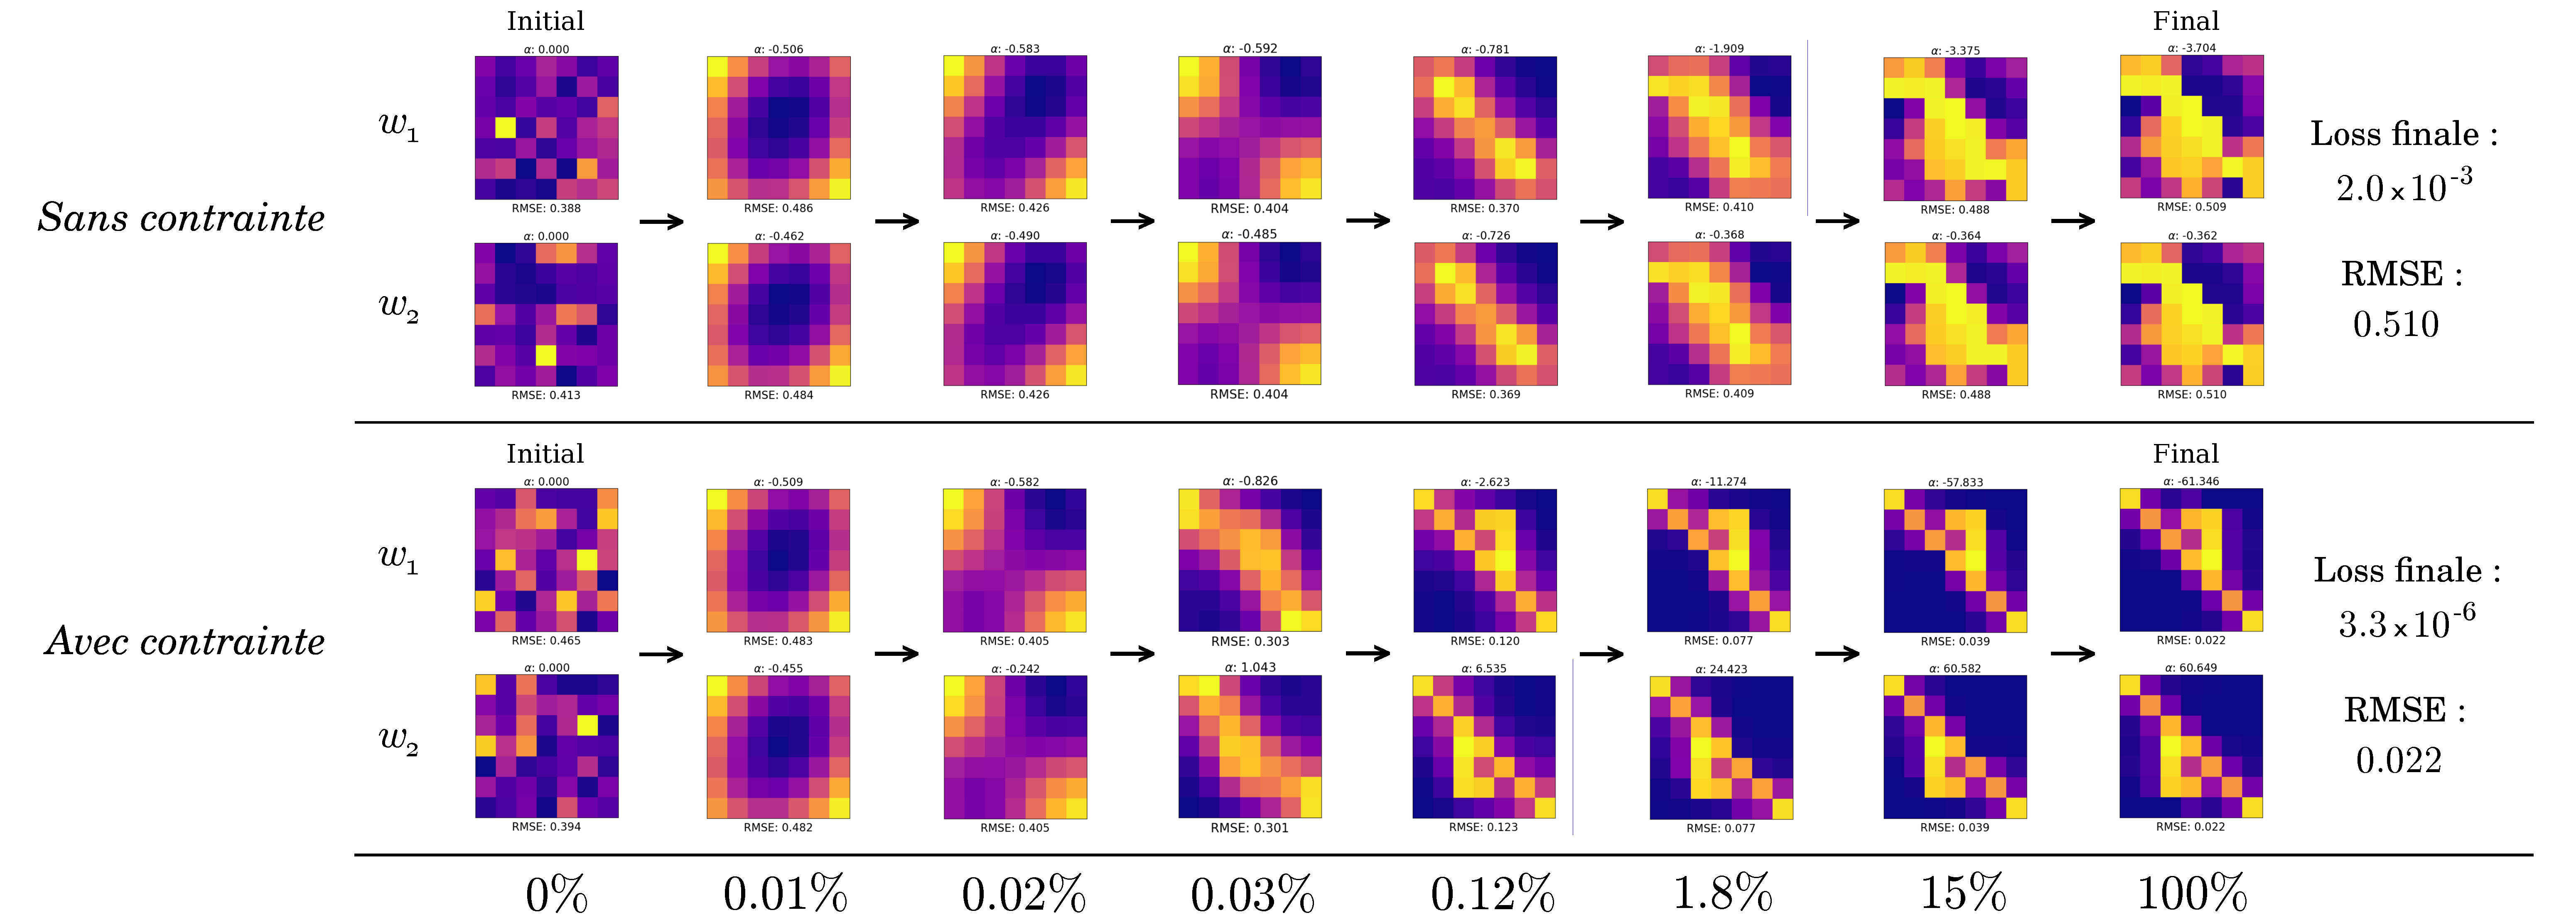
\includegraphics[width=1.00\linewidth]{parts/3-contributions/C-contraintes_geometriques/figures/k_awayOPP.pdf}
    \vspace{-4.0mm}
    \caption{ \centering Évolution de la forme du noyau des deux couches du réseau et de sa \textit{RMSE} en fonction de la progression de l'entraînement (en \% avant l'état final), pour le \textit{adiag} et l'ouverture sur la banque MNIST, avec et sans la contrainte $C_\text{awayOPP}$.}
    \label{fig:c_awayOPP}
  \end{center}
\end{figure}

\vspace{-3.6mm}
\noindent Comme le montrent les résultats de cet exemple, cette métrique est très performante dans les échecs de convergence où les $\alpha$ sont de même signe alors qu'ils ne le devraient pas. Cependant, il faut garder à l'esprit le fait que cette métrique ne peut être utilisée que si on sait à priori que les deux $\alpha$ doivent être de signe opposé.

\newpage

\subsubsection{Application et comparaison de l'efficacité}
\vspace{0.2cm}
À partir de ces différentes contraintes définies précédemment, celles sur les noyaux $w$ et celles sur les paramètres de contrôle $\alpha$ des couches morphologiques, on crée finalement une \textit{loss} personnalisable, dans laquelle on ajoute les contraintes que l'on souhaite, chacune pondérée par un hyperparamètre propre à elle-même. C'est à l'utilisateur de choisir les contraintes à intégrer selon les contextes, selon la géométrie visée des noyaux du réseau, et selon les valeurs des $\alpha$ recherchées. Cependant, plus il y a de contraintes différentes ajoutées dans la fonction de perte \textit{loss}, plus le réseau aura tendance à << délaisser >> certaines contraintes pour d'autres, lors de son entraînement, et moins le réseau convergera bien et sera performant à la fin. \\

\vspace{-1.6mm}
\noindent Dans notre cas, les huit fonctions structurantes cibles étudiées ayant des propriétés géométriques bien différentes, l'application d'une même contrainte géométrique parmi celles développées n'est pas adaptée. On peut cependant, dans le cadre des échecs de la partie précédente sur les réseaux à deux couches, faire l'hypothèse forte (que l'on n'utilisera pas dans des contextes où l'on ignore l'hypothèse) que l'on veut que les réseaux se comportent soit comme une ouverture, soit comme une fermeture. On prend ainsi la seconde contrainte sur les paramètres de contrôle $\alpha$, l'erreur sur l'éloignement opposé (formule \ref{erreur_awayOPP}), qu'on applique sur l'ensemble des expériences de la partie précédente, avec toujours un partage de poids doux en plus. \\

\vspace{-1.6mm}
En reprennant la même méthodologie que dans les parties précédentes avec des réseaux $\mathcal{S}$MorphNetTanh à deux couches, on obtient, pour l'opération cible d'ouverture et la banque d'images d'entraînement MNIST, les résultats suivants (fig. \ref{fig:MSEpFSIMvsMSEpFSIMpASIM_opening}) : \\

% figure
\vspace{1.0mm}
\begin{figure}[!htp]
  \begin{center}
  
    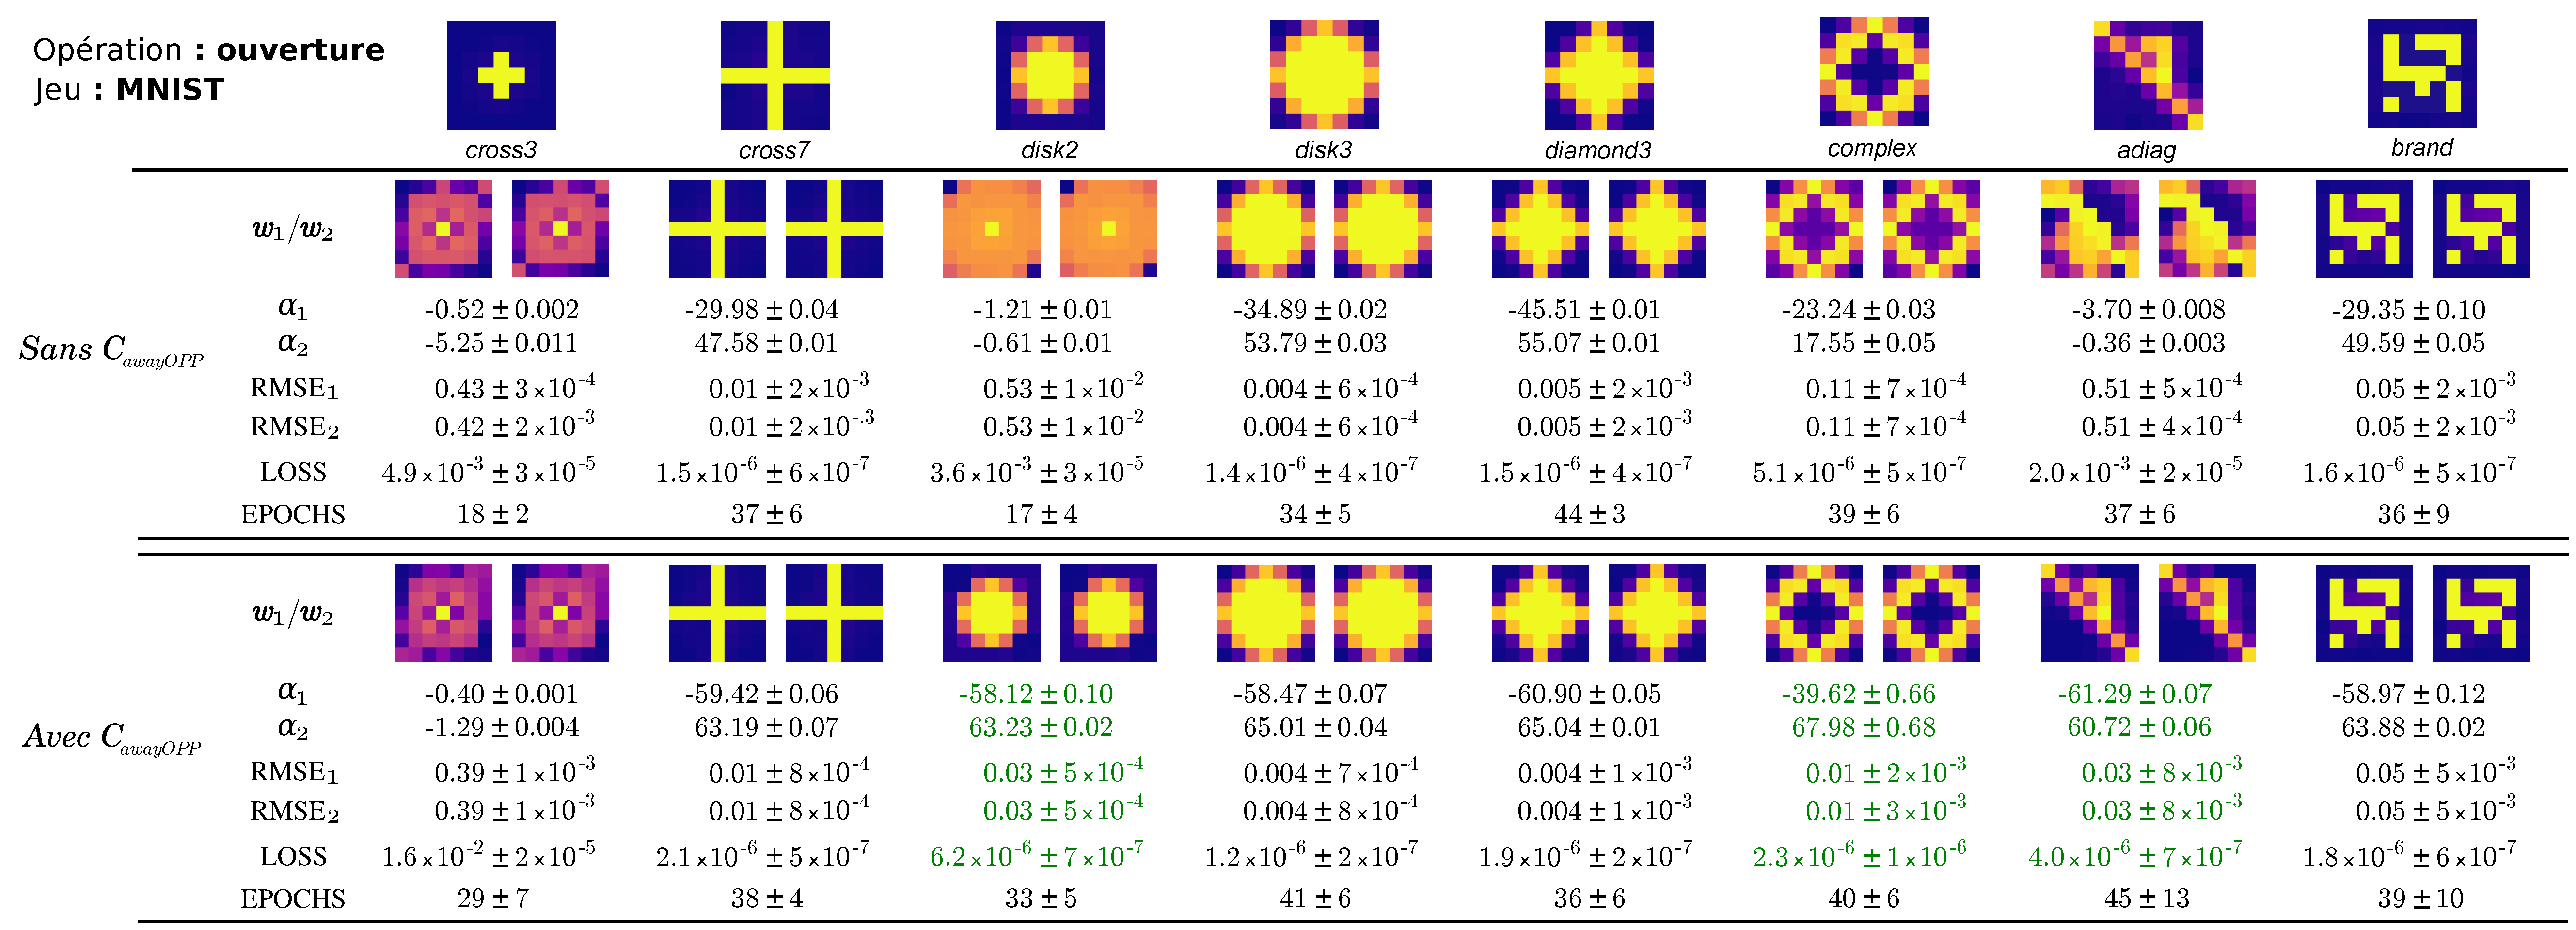
\includegraphics[width=1.00\linewidth]{parts/3-contributions/C-contraintes_geometriques/figures/f_opening_mnist.pdf}
    \vspace{-4.0mm}
    \caption{ \centering Comparaison des poids appris et des moyennes et écarts-types des métriques $\alpha$, \textit{RMSE}, \textit{loss} et nombre d'époques, et ce sur six runs, entre sans et avec la contrainte $C_\text{awayOPP}$, pour les huit fonctions structurantes cibles et l'opération d'\textbf{ouverture}.}
    \label{fig:MSEpFSIMvsMSEpFSIMpASIM_opening}
    
  \end{center}
\end{figure}


\newpage

On obtient également, pour l'opération cible de fermeture et la banque MNIST avec des réseaux $\mathcal{S}$MorphNetTanh à deux couches, les résultats suivants (fig. \ref{fig:MSEpFSIMvsMSEpFSIMpASIM_closing}) : \\

% figure
\vspace{1.6mm}
\begin{figure}[!htp]
  \begin{center}
  
    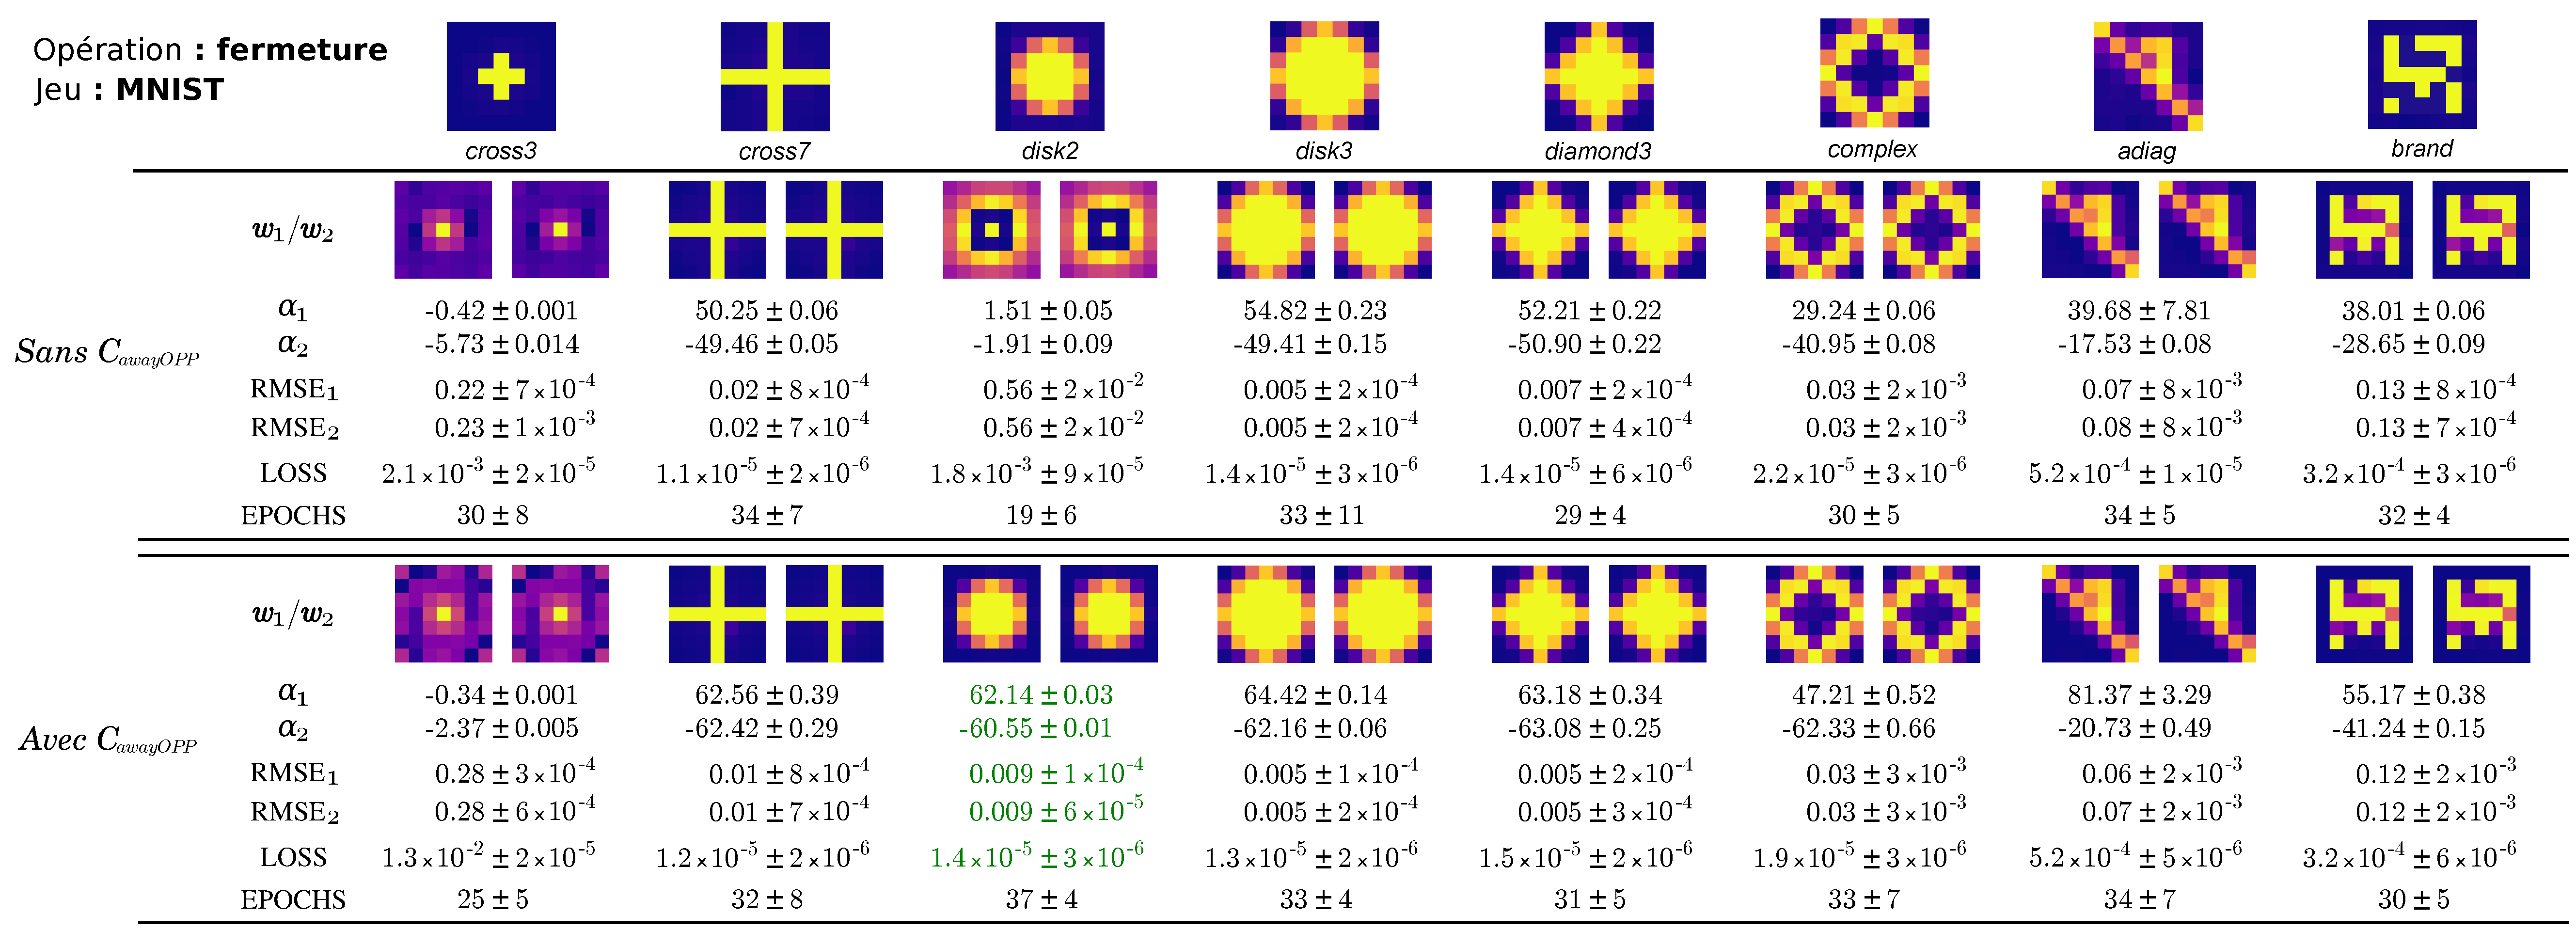
\includegraphics[width=1.00\linewidth]{parts/3-contributions/C-contraintes_geometriques/figures/f_closing_mnist.pdf}
    \vspace{-4.0mm}
    \caption{ \centering Comparaison des poids appris et des moyennes et écarts-types des métriques $\alpha$, \textit{RMSE}, \textit{loss} et nombre d'époques, et ce sur six runs, entre sans et avec la contrainte $C_\text{awayOPP}$, pour les huit fonctions structurantes cibles et l'opération de \textbf{fermeture}.}
    \label{fig:MSEpFSIMvsMSEpFSIMpASIM_closing}
    
  \end{center}
\end{figure}


\vspace{-1.0mm}
Les résultats de convergence de $\mathcal{S}$MorphNetTanh sur les figures \ref{fig:MSEpFSIMvsMSEpFSIMpASIM_opening} et \ref{fig:MSEpFSIMvsMSEpFSIMpASIM_closing}, montrant l'état final des noyaux des réseaux et les valeurs des métriques de performances associées pour les différentes expériences réalisées, permettent de mettre en évidence l'efficacité de la métrique de contrainte $C_\text{awayOPP}$, qui influe sur les paramètres de contrôle $\alpha$, et qui est ici associée à un partage de poids doux, dans le cadre d'une opération cible d'ouverture (\ref{fig:MSEpFSIMvsMSEpFSIMpASIM_opening}) et de fermeture (\ref{fig:MSEpFSIMvsMSEpFSIMpASIM_closing}) sur des réseaux à deux couches. \\

\vspace{-0.6mm}
\noindent Les résultats en couleur verte sont ceux pour lesquels les réseaux avec cette contrainte $C_\text{awayOPP}$ ont de bien meilleurs résultats. Cela concerne en particulier les expériences avec \textit{disk2}, \textit{complex} et \textit{adiag} pour l'ouverture, et l'expérience avec \textit{disk2} pour la fermeture. On obtient les mêmes résultats avec les expériences faites sur FashionMNIST. Pour ces expériences-là, la contrainte $C_\text{awayOPP}$ couplée à un partage de poids doux a permis au réseau de bien converger vers l'état cible, avec une forme des noyaux proche de celle de la fonction structurante cible, et avec des valeurs de $\alpha$ du bon signe et éloignées de $0$ (on a donc plus une opération exacte qu'une pseudo-opération). \\

\vspace{-0.6mm}
\noindent Cependant, on remarque qu'il existe toujours une fonctions structurante cible pour laquelle cette contrainte n'a pas d'impact, et ce à la fois pour l'ouverture et la fermeture : \textit{cross3}. En examinant les valeurs de $\alpha$, on remarque qu'elles restent très proches de $0$ et sont du même signe, malgré la présence de la contrainte $C_\text{awayOPP}$. Elle n'est donc pas encore suffisante pour améliorer la convergence de l'ensemble des échecs.

\newpage

% Initialisation gaussienne
\subsection{Modulation de l'initialisation} %Partage de poids

\subsubsection{Motivations et principe}
\vspace{0.2cm}
Les résultats précédents montrent qu'il reste encore quelques cas d'échecs de convergence pour les réseaux $\mathcal{S}$MorphNetTanh à deux couches morphologiques, avec les opérations cibles d'ouverture et de fermeture, et ce malgré l'ajout d'un partage doux des poids entre les noyaux $w$ des deux couches et l'ajout dans la \textit{loss} d'une contrainte $C_\text{awayOPP}$ entre les deux paramètres de contrôle $\alpha$ (ou $p$) associés. \\

\vspace{-1.4mm}
\noindent La modulation de l'initialisation des noyaux $w$ du réseau devient alors une solution potentielle à ces derniers échecs. ALors que les poids des noyaux sont originellement initialisés selon une loi normale centrée réduite afin de brasser les différents états de convergence possibles à partir d'initialisations aléatoires différentes sur plusieurs expériences, on peut finalement se dire que cette forme initiale des noyaux peut être fixée et définie de manière déterminée au préalable, selon des caractéristiques morphologiques générales à priori que l'on connait ou que l'on recherche sur ces noyaux. \\

\vspace{-1.4mm}
\noindent En l'occurence, on peut facilement s'imaginer que ce que l'on recherche ou favorise dans nos différents cas d'étude, c'est une forme de noyaux centrée sur son support et peu dispersée. On choisira alors une initialisation sous la forme d'une gaussienne 2D, allant de $0$ aux coins de l'image des noyaux à $1$ en son centre (voir figure \ref{fig:init_gauss} suivante). \\


%figure
\vspace{-1.0mm}
\begin{figure}[htp]
  \begin{center}
    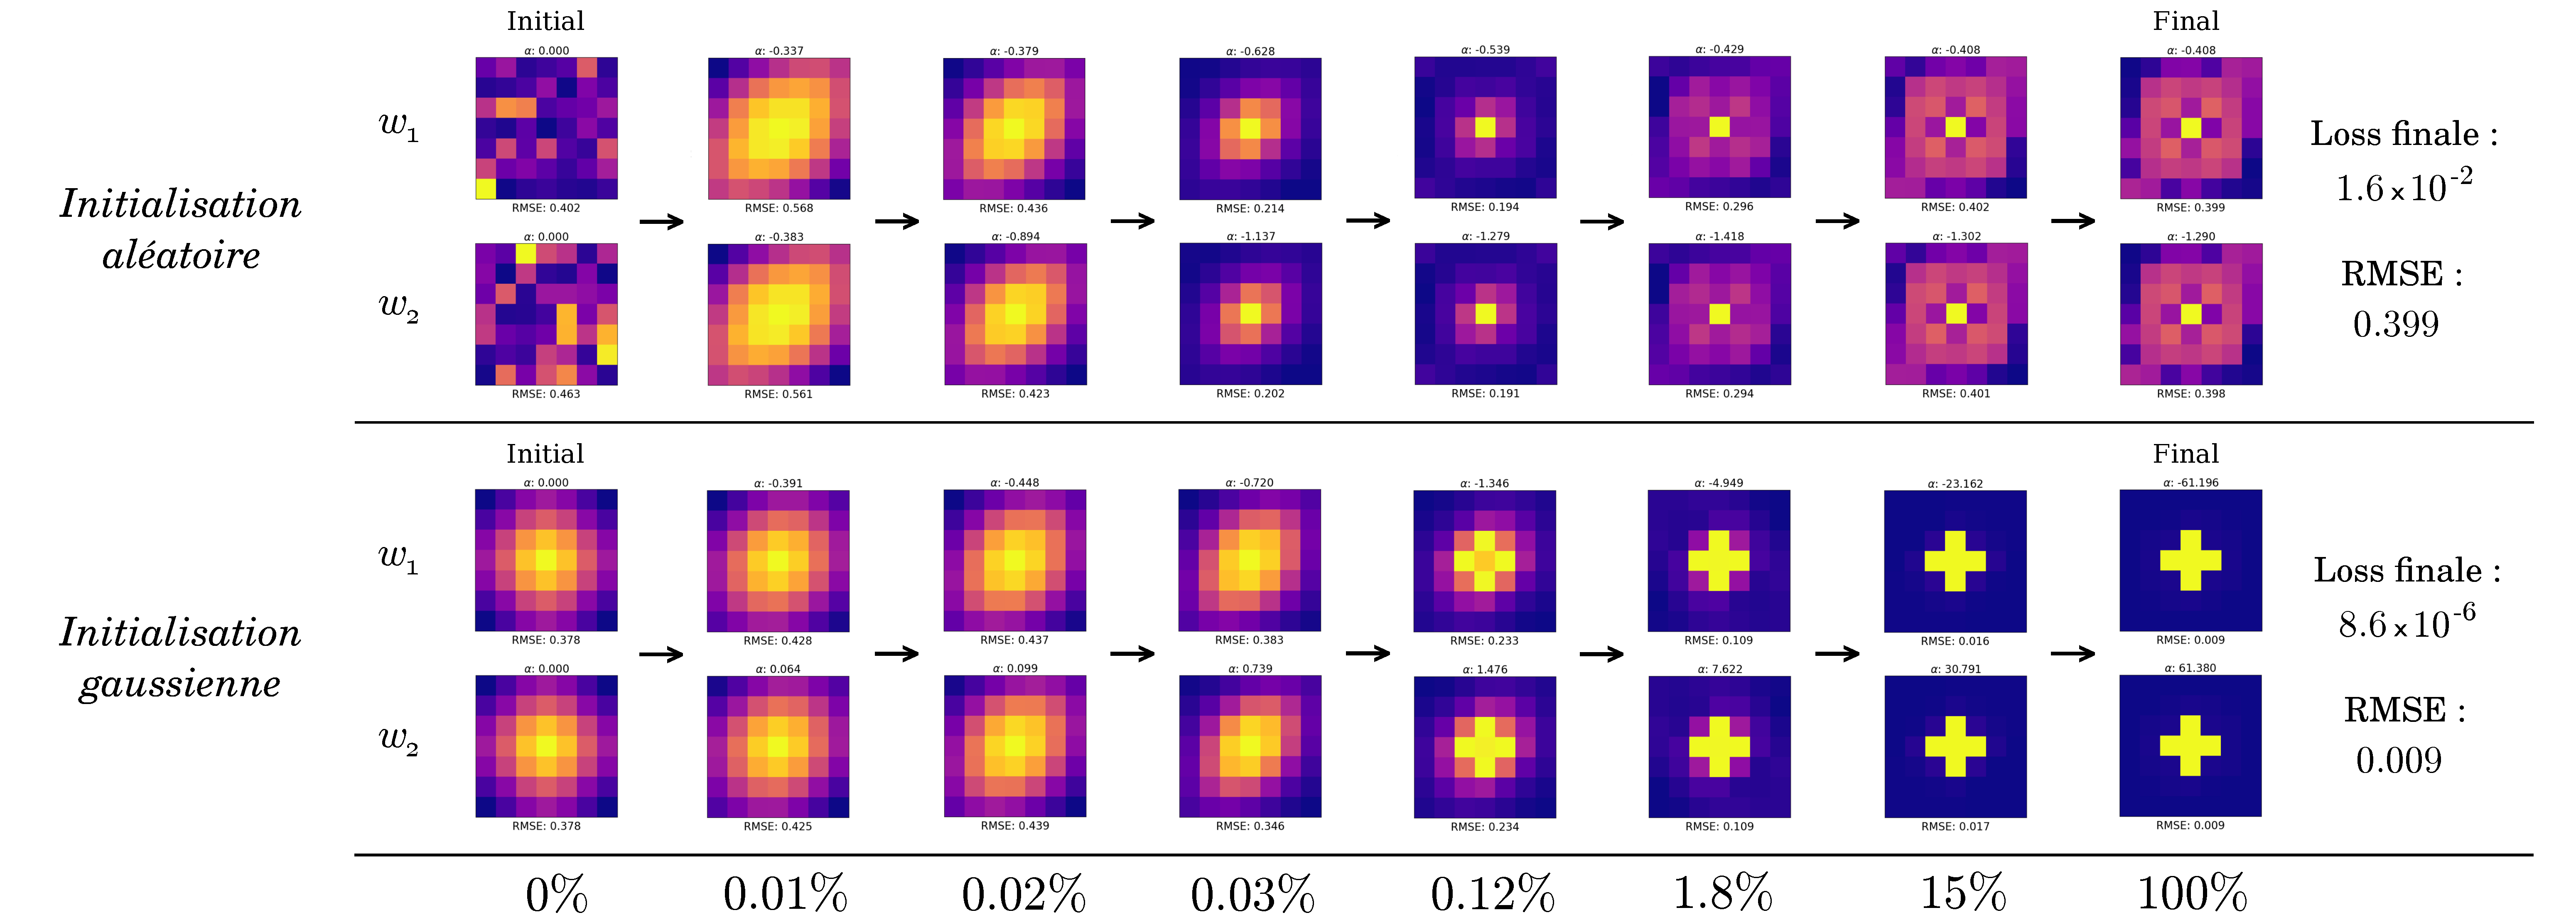
\includegraphics[width=1.00\linewidth]{parts/3-contributions/D-modulation_de_l_initialisation/figures/k_gauss.pdf}
    \vspace{-4.0mm}
    \caption{ \centering Évolution de la forme du noyau des deux couches du réseau et de sa \textit{RMSE} en fonction de la progression de l'entraînement (en \% avant l'état final), pour le \textit{cross3} et l'ouverture sur la banque MNIST, avec initialisation aléatoire et init. gaussienne.}
    \label{fig:init_gauss}
  \end{center}
\end{figure}


\vspace{-3.0mm}
\noindent L'exemple fig. \ref{fig:init_gauss}, obtenu sur six runs, montre bien ici l'efficacité de cette initialisation gaussienne des noyaux $w$ par rapport à l'aléatoire normale centrée réduite sur \textit{cross3} pour l'ouverture sur MNIST, avec des valeurs de \textit{RMSE} et de \textit{loss} bien plus faibles.

\newpage

\subsubsection{Comparaison de l'efficacité}
\vspace{0.2cm}
La première expérience avec la fonction structurante cible \textit{cross3} pour l'opération cible d'ouverture et avec la banque d'images d'entraînement MNIST, expérience pour laquelle le réseau ne converge originellement pas avec une initialisation aléatoire des poids des noyaux $w$ issue d'une loi normale centrée réduite, s'avère ici être un succès grâce à l'initialisation gaussienne 2D de ces noyaux (voir figure précédente \ref{fig:init_gauss}). 
Cependant, pour estimer avec davantage de certitude l'efficacité globale de cette modulation de l'initialisation des noyaux $w$ des couches du réseau, il faut observer son impact sur l'ensemble des expériences de notre étude, donc également sur les expériences qui sont originellement un succès avec une initialisation aléatoire des $w$. \\

\vspace{-1.0mm}
\noindent Considérons alors ici le même paramétrage du réseau $\mathcal{S}$MorphNetTanh à deux couches morphologiques que dans la partie précédente, c'est-à-dire munie, dans la fonction de perte \textit{loss}, d'un partage de poids doux entre les noyaux $w$ de ses deux couches (formule \ref{Csim3}), et de la contrainte $C_\text{awayOPP}$ sur l'éloignement opposé entre ses deux paramètres de contrôle $\alpha$ respectifs (formule \ref{erreur_awayOPP}). On modifie donc simplement ici, sur l'ensemble des expériences de notre étude, l'initialisation des poids des noyaux $w$ par une gaussienne 2D telle que décrite précédemment (illustrée fig. \ref{fig:init_gauss} en début d'entraînement, sur la seconde ligne, à 0\%), et les résultats de convergence issus de cette initialisation déterministe sont comparés à ceux issus de l'initialisation aléatoire. \\

\vspace{-1.0mm}
En reprenant donc la même méthodologie que précédemment avec des réseaux $\mathcal{S}$MorphNetTanh à deux couches, on obtient, pour l’opération cible d’ouverture et la banque d’images d’entraînement MNIST, les résultats suivants (fig. \ref{fig:RANDvsGAUSS_opening}) : \\


% figure
\vspace{0.1mm}
\begin{figure}[!htp]
  \begin{center}
    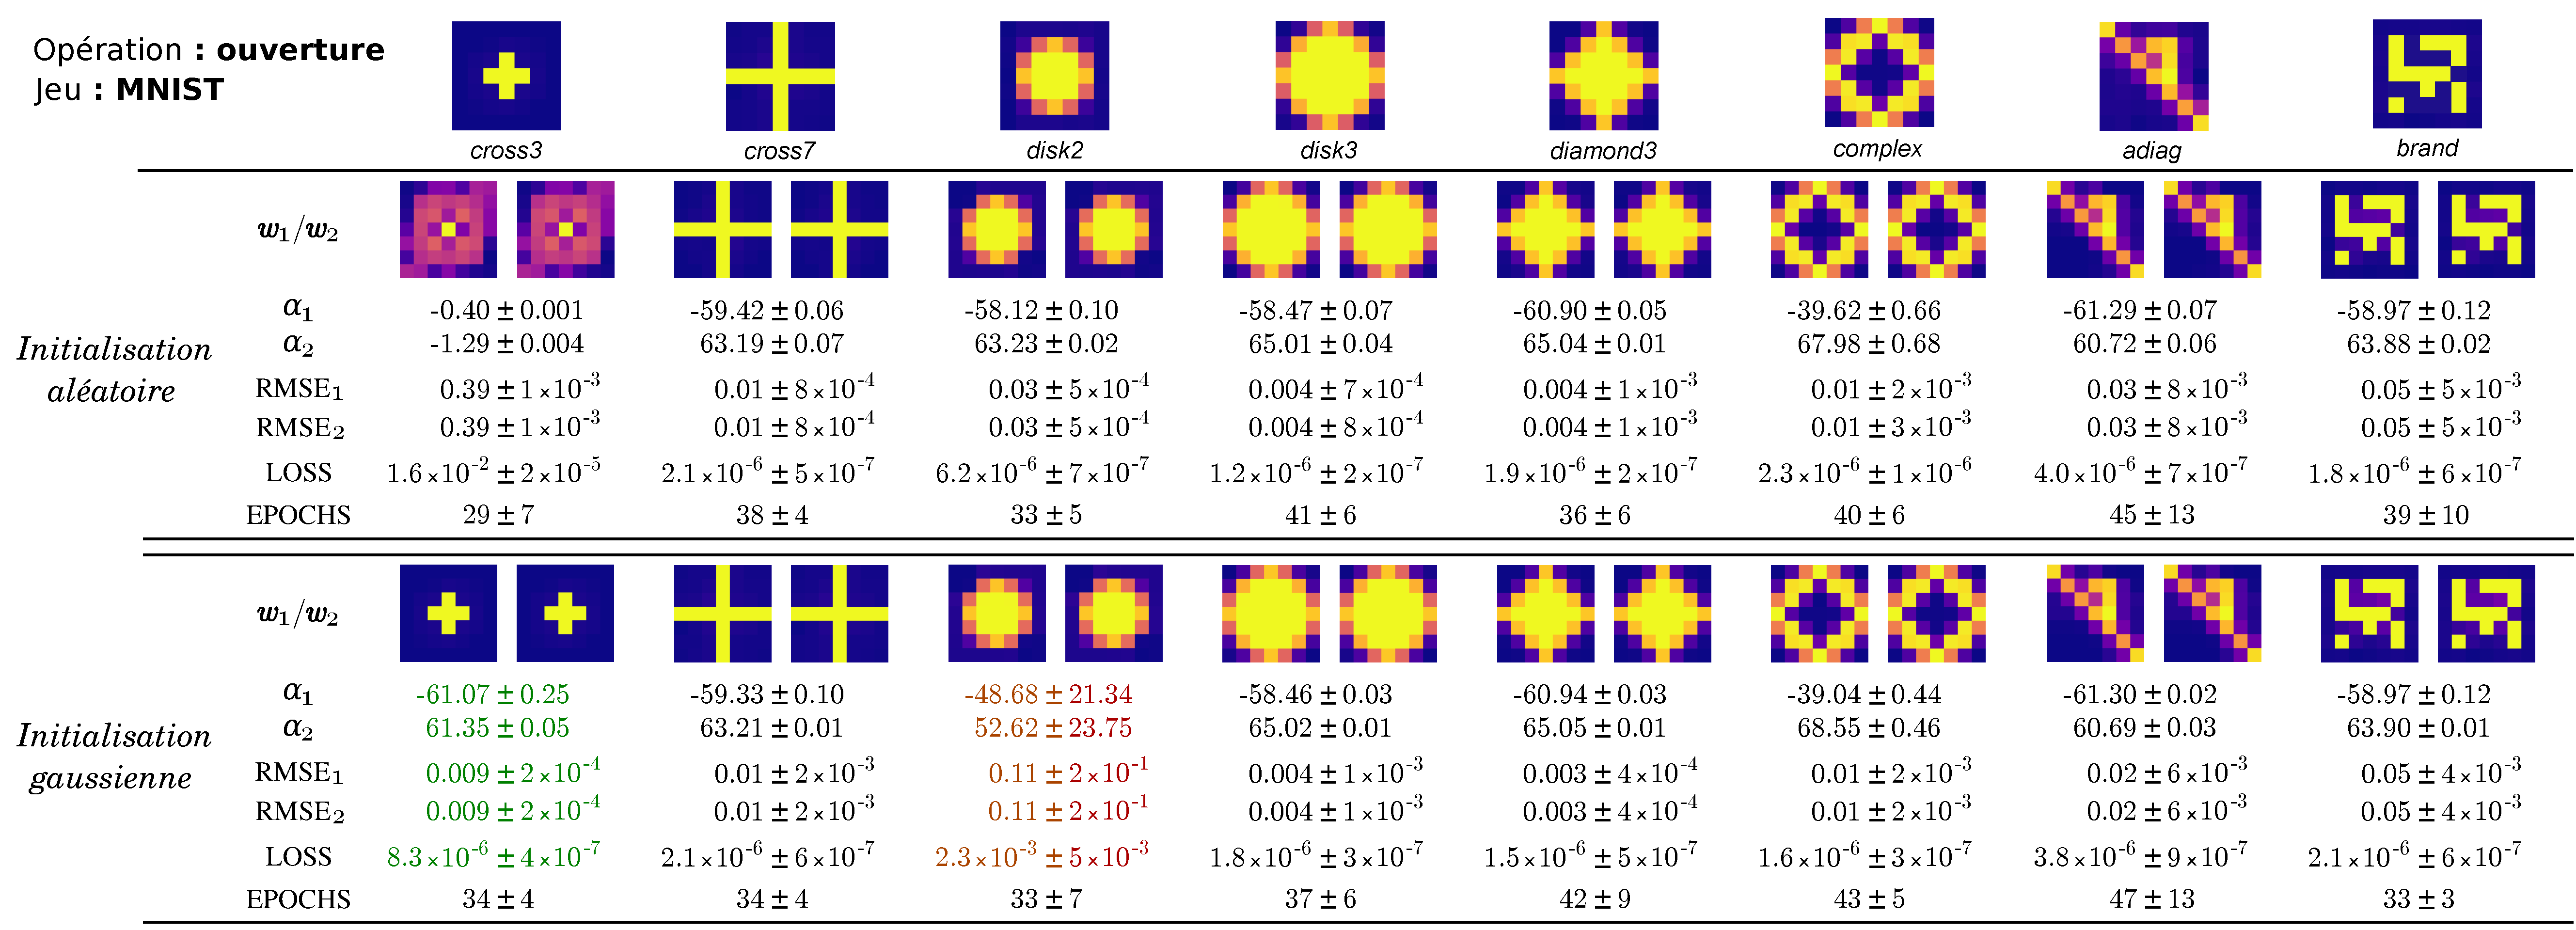
\includegraphics[width=1.00\linewidth]{parts/3-contributions/D-modulation_de_l_initialisation/figures/g_opening_mnist.pdf}
    \vspace{-4.0mm}
    \caption{ \centering Comparaison des poids appris et des moyennes et écarts-types des métriques $\alpha$, \textit{RMSE}, \textit{loss} et nombre d'époques, et ce sur six runs, entre initialisation aléatoire et gaussienne, pour les huit fonctions structurantes cibles et l'opération d'\textbf{ouverture}.}
    \label{fig:RANDvsGAUSS_opening}
  \end{center}
\end{figure}


\newpage

On obtient également, pour l’opération cible de fermeture et la banque MNIST avec des réseaux $\mathcal{S}$MorphNetTanh à deux couches, les résultats suivants (fig. \ref{fig:RANDvsGAUSS_closing}) : \\

%figure
\vspace{0.2mm}
\begin{figure}[!htp]
  \begin{center}
    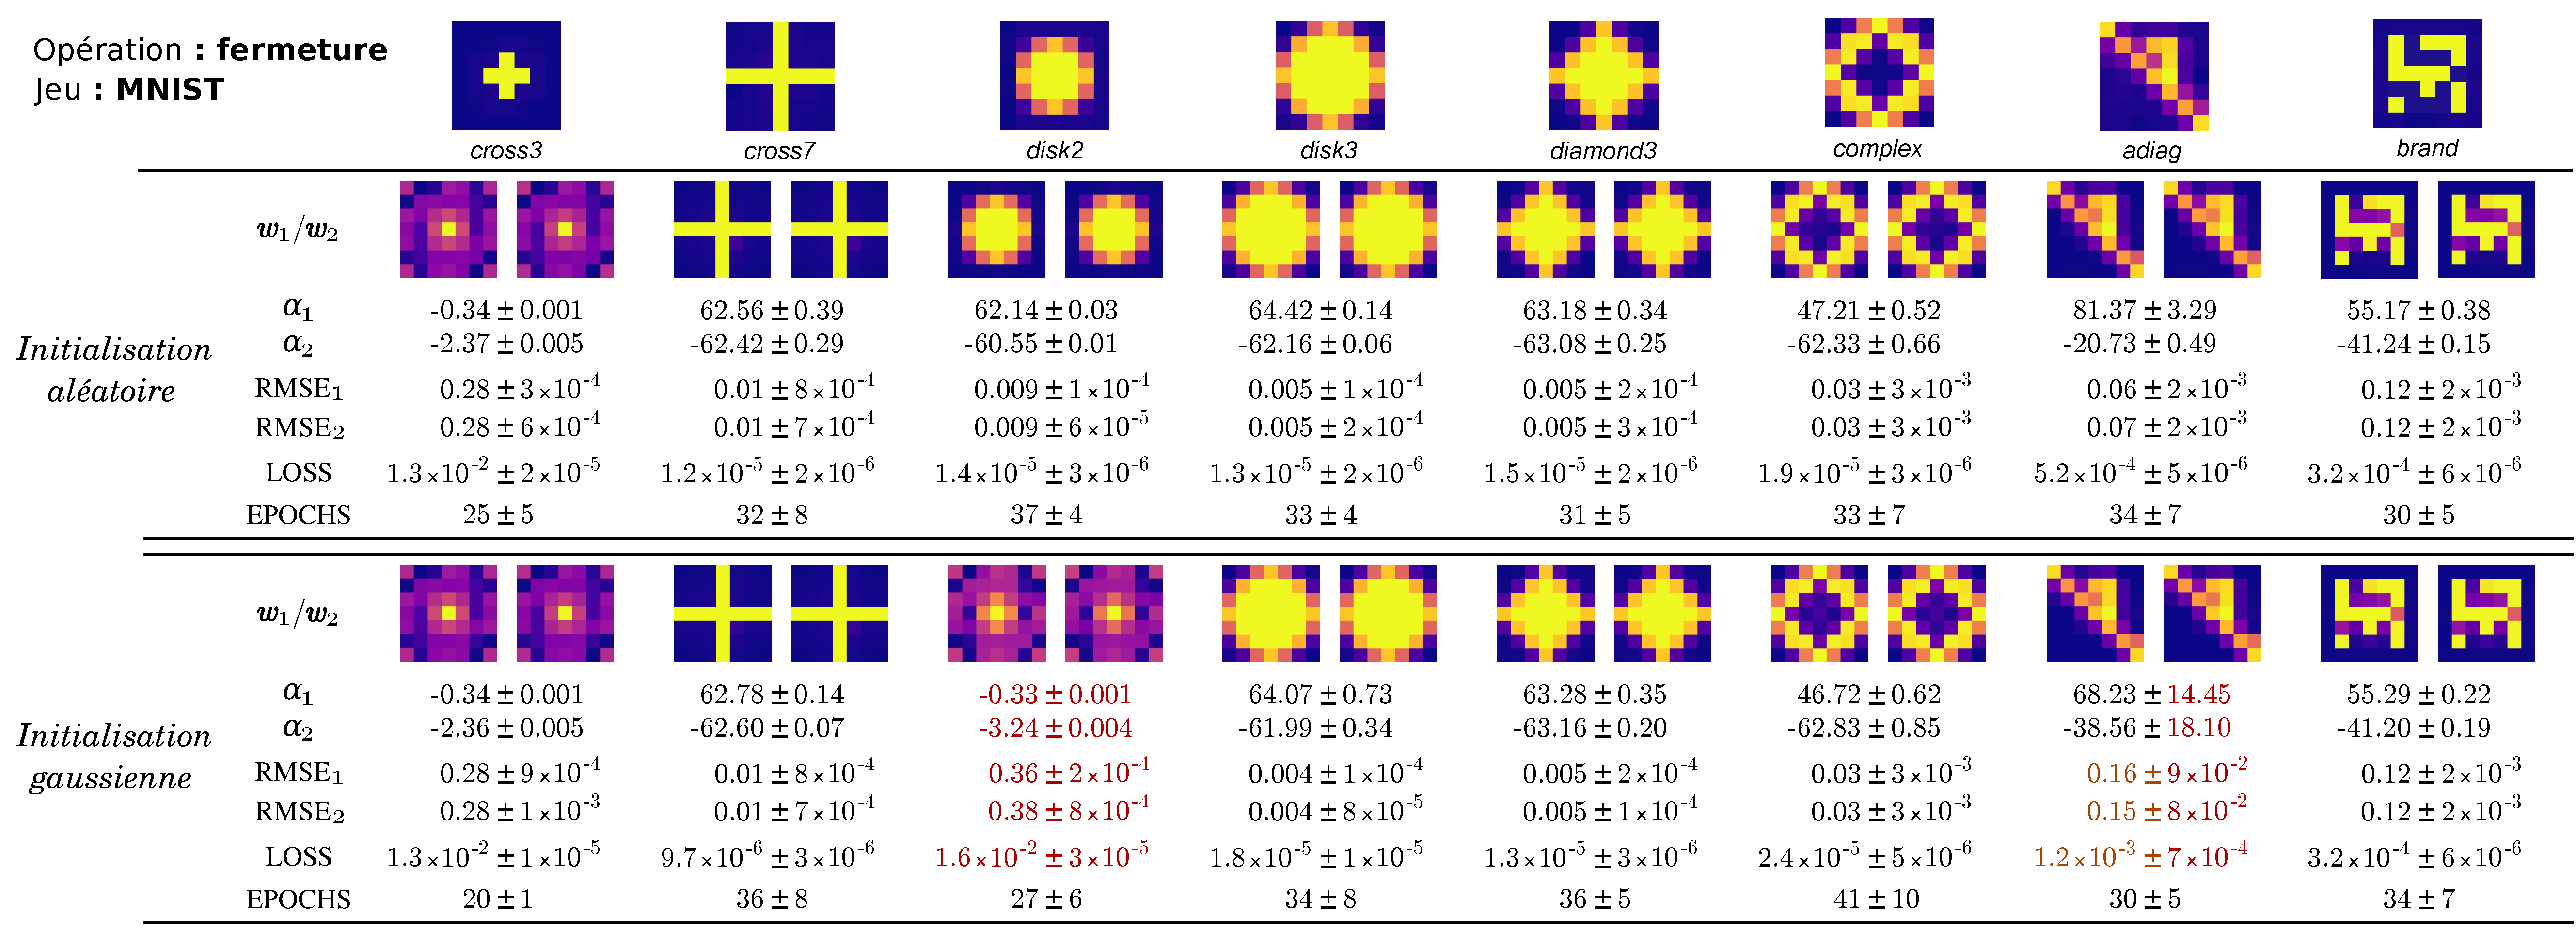
\includegraphics[width=1.00\linewidth]{parts/3-contributions/D-modulation_de_l_initialisation/figures/g_closing_mnist.pdf}
    \vspace{-4.0mm}
    \caption{ \centering Comparaison des poids appris et des moyennes et écarts-types des métriques $\alpha$, \textit{RMSE}, \textit{loss} et nombre d'époques, et ce sur six runs, entre initialisation aléatoire et gaussienne, pour les huit fonctions structurantes cibles et l'opération de \textbf{fermeture}.}
    \label{fig:RANDvsGAUSS_closing}
  \end{center}
\end{figure}


\vspace{-2.0mm}
Les données en rouge illustrent les cas où l'initialisation gaussienne donne de moins bons résultats que l'initialisation aléatoire, tandis que ceux en vert illustrent, à inverses, les cas où c'est l'initialisation gaussienne qui donne de meilleurs résultats. \\ %que l'aléatoire.

\vspace{-2.2mm}
\noindent On remarque en effet que l'expérience avec \textit{cross3} pour l'ouverture avec MNIST est un net succès pour l'initialisation gaussienne contrairement à l'initialisation aléatoire, aussi bien en terme visuel avec une grande ressemblance des noyaux $w$ par rapport à la structure cible \textit{cross3}, qu'en termes de valeurs des métriques de performances, avec une \textit{RMSE} bien plus faible pour les deux noyaux $w$, une forte valeur absolue des deux paramètres de contrôle $\alpha$ avec le bon signe, et une perte globale \textit{loss} mineure. \\

\vspace{-2.2mm}
\noindent Cependant, il s'agit là de la seule expérience dont les résultats sont meilleurs avec l'initialisation gaussienne. Il y a, à l'inverse, plusieurs expériences qui ont cette fois moins bien convergé avec une telle initialisation, telles que celles avec \textit{disk2} à la fois pour l'ouverture et la fermeture, ou encore celle avec \textit{adiag} pour la fermeture (qui a des écarts-types élevés, illustrant l'échec de certaines runs), sur MNIST. Certains succès avec une initialisation aléatoire sont ainsi devenus des échecs avec la gaussienne. \\

\vspace{-1.6mm}
En conclusion, on ne peut pas dire que l'initialisation aléatoire donne de meilleurs résultats de convergence sur ces réseaux, d'autant plus que l'on obtient les mêmes résultats, voir pires, avec la banque FashionMNIST. On s'interroge en particulier sur la raison de l'échec des expériences avec la structure cible \textit{disk2}, qui a pourtant une forme visuelle proche de la gaussienne 2D utilisée pour l'initialisation des noyaux $w$.

\newpage

%========================================================================================
%	4. ANALYSE GLOBALE DES RESEAUX
%========================================================================================

\section{Analyse des réseaux}

% 2 couches pour 1 opération morphologique primaire
\subsection{Réseaux à deux couches pour une opération primaire}

\subsubsection{Motivations}
\vspace{0.2cm}
Les réseaux morphologiques sont construits sous l'architecture telle que décrite et présentée dans la partie état de l'art, figure \ref{fig:architecture_reseau_morpho}, avec $n$ couches morphologiques du type considéré ($p$Conv, $\mathcal{L}$Morph, $\mathcal{S}$Morph/Tanh), disposées successivement entre une standardisation au début du réseau et une couche de convolution de taille 1x1x1 en fin du réseau. En l'occurence, pour les réseaux $\mathcal{S}$MorphNet (resp. $\mathcal{S}$MorphNetTanh) que l'on considère ici, le réseau possèdera $n$ couches $\mathcal{S}$Morph (resp. $\mathcal{S}$MorphTanh). \\

\vspace{-1.2mm}
\noindent Comme vu dans les parties précédentes, chaque couche morphologique, par sa définition, ne pourra avoir l'effet que d'une (pseudo-)opération morphologique \textit{primaire}, à savoir soit celle d'une \textit{érosion} soit celle d'une \textit{dilatation}, définie en fonction de ka valeur du paramètre de contrôle $\alpha$ (ou $p$) de la couche. En particulier, si $\alpha$ (ou $p$) tend vers $- \infty$, alors l'effet de la couche tendra vers celle d'une érosion exacte, et si $\alpha$ (ou $p$) tend vers $+ \infty$, alors son effet tendra vers celle d'une dilatation exacte. \\

\vspace{-1.2mm}
\noindent De ce fait, pour que le réseau en lui-même puisse avoir l'effet, sur les images en entrée, d'une opération primaire, une seule et unique couche morphologique suffit au sein de ce réseau. Pour qu'il ait l'effet d'une ouverture ou d'une fermeture, qui sont tous deux la composition de deux opérations primaires successives, on munira naturellement le réseau de deux couches morphologiques, en espérant que chacune tende soit vers l'érosion exacte soit vers la dilatation exacte. \\

\vspace{0.6mm}
\noindent Vient alors une question : que se passe-t-il si l'on munit le réseau de plusieurs couches morphologiques successives, deux par exemple, pour une opération cible \textit{primaire} ? \\

\vspace{1.0mm}
On souhaiterait ici comprendre comment le réseau se comporterait dans une telle configuration. On aimerait savoir s'il arriverait à trouver une décomposition exacte de l'élément (ou fonction) structurant cible en deux éléments successifs, et s'il arriverait à converger correctement (avec des paramètres de contrôle $\alpha / p$ de grande amplitude, et une valeur de \textit{loss} faible sur les prédictions faites). Par exemple, une décomposition exacte d'une érosion ou d'une dilatation par un élément structurant \textit{carré} de taille 3x3 est la même opération successive par un segment vertical de longueur 3 (et de largeur 1) puis par un segment horizontal de même taille, ou bien inversement. \\

\vspace{-1.2mm}
\noindent On décomposera cette analyse en deux partie : celle pour l'opération cible d'\textit{érosion} sur un réseau à deux couches, et celle pour l'opération cible de \textit{dilatation} sur un réseau à deux couches. On considérera ici les réseaux $\mathcal{S}$MorphNet et $\mathcal{S}$MorphNetTanh.

\newpage

\subsubsection{Avec l'érosion}
\vspace{0.2cm}
Commençons d'abord cette analyse avec l'opération cible d'érosion. On munit un réseau $\mathcal{S}$MorphNetTanh classique de deux couches morphologiques, sans partage de poids et sans contrainte (on considère la fonction de perte \textit{loss} classique, c'est-à-dire seulement la MSE entre les images cibles et les prédictions du réseau), et on l'entraîne sur la banque MNIST avec les huit fonctions structurantes cibles de nos études précédentes, et avec toujours l'opération cible d'\textit{érosion}. On ajoute également à ces huit fonctions structurantes la nouvelle structure binaire carrée de taille 3x3, qui nous intéresse dans cette étude afin de voir si le réseau peut par exemple la décomposer en deux segments, un vertical et un horizontal, comme expliqué précédemment. \\

\vspace{-1.0mm}
\noindent En lançant l'entraînement des différentes expériences, on remarque que l'ensemble des résultats de convergence se divisent en deux parties : celle dans laquelle les noyaux du réseau ont convergé vers une forme distinguable et harmonieuse avec une valeur de perte \textit{loss} faible (le réseau a << bien >> convergé, c'est un << succès >>), et celle dans laquelle les noyaux ont convergé vers une forme peu distinguable et peu harmonieuse, avec en général des valeurs de paramètre de contrôle $\alpha$ proches de 0, et avec une valeur de \textit{loss} élevée (le réseau a << mal >> convergé, c'est un << échec >>).
En prenant l'exemple du carré de taille 3x3, on obtient une << mauvaise >> convergence, dont l'état final des deux couches est la suivante, illustrée figure \ref{fig:square_fail} : \\

%figure
\vspace{1.6mm}
\begin{figure}[!htp]
  \begin{center}
    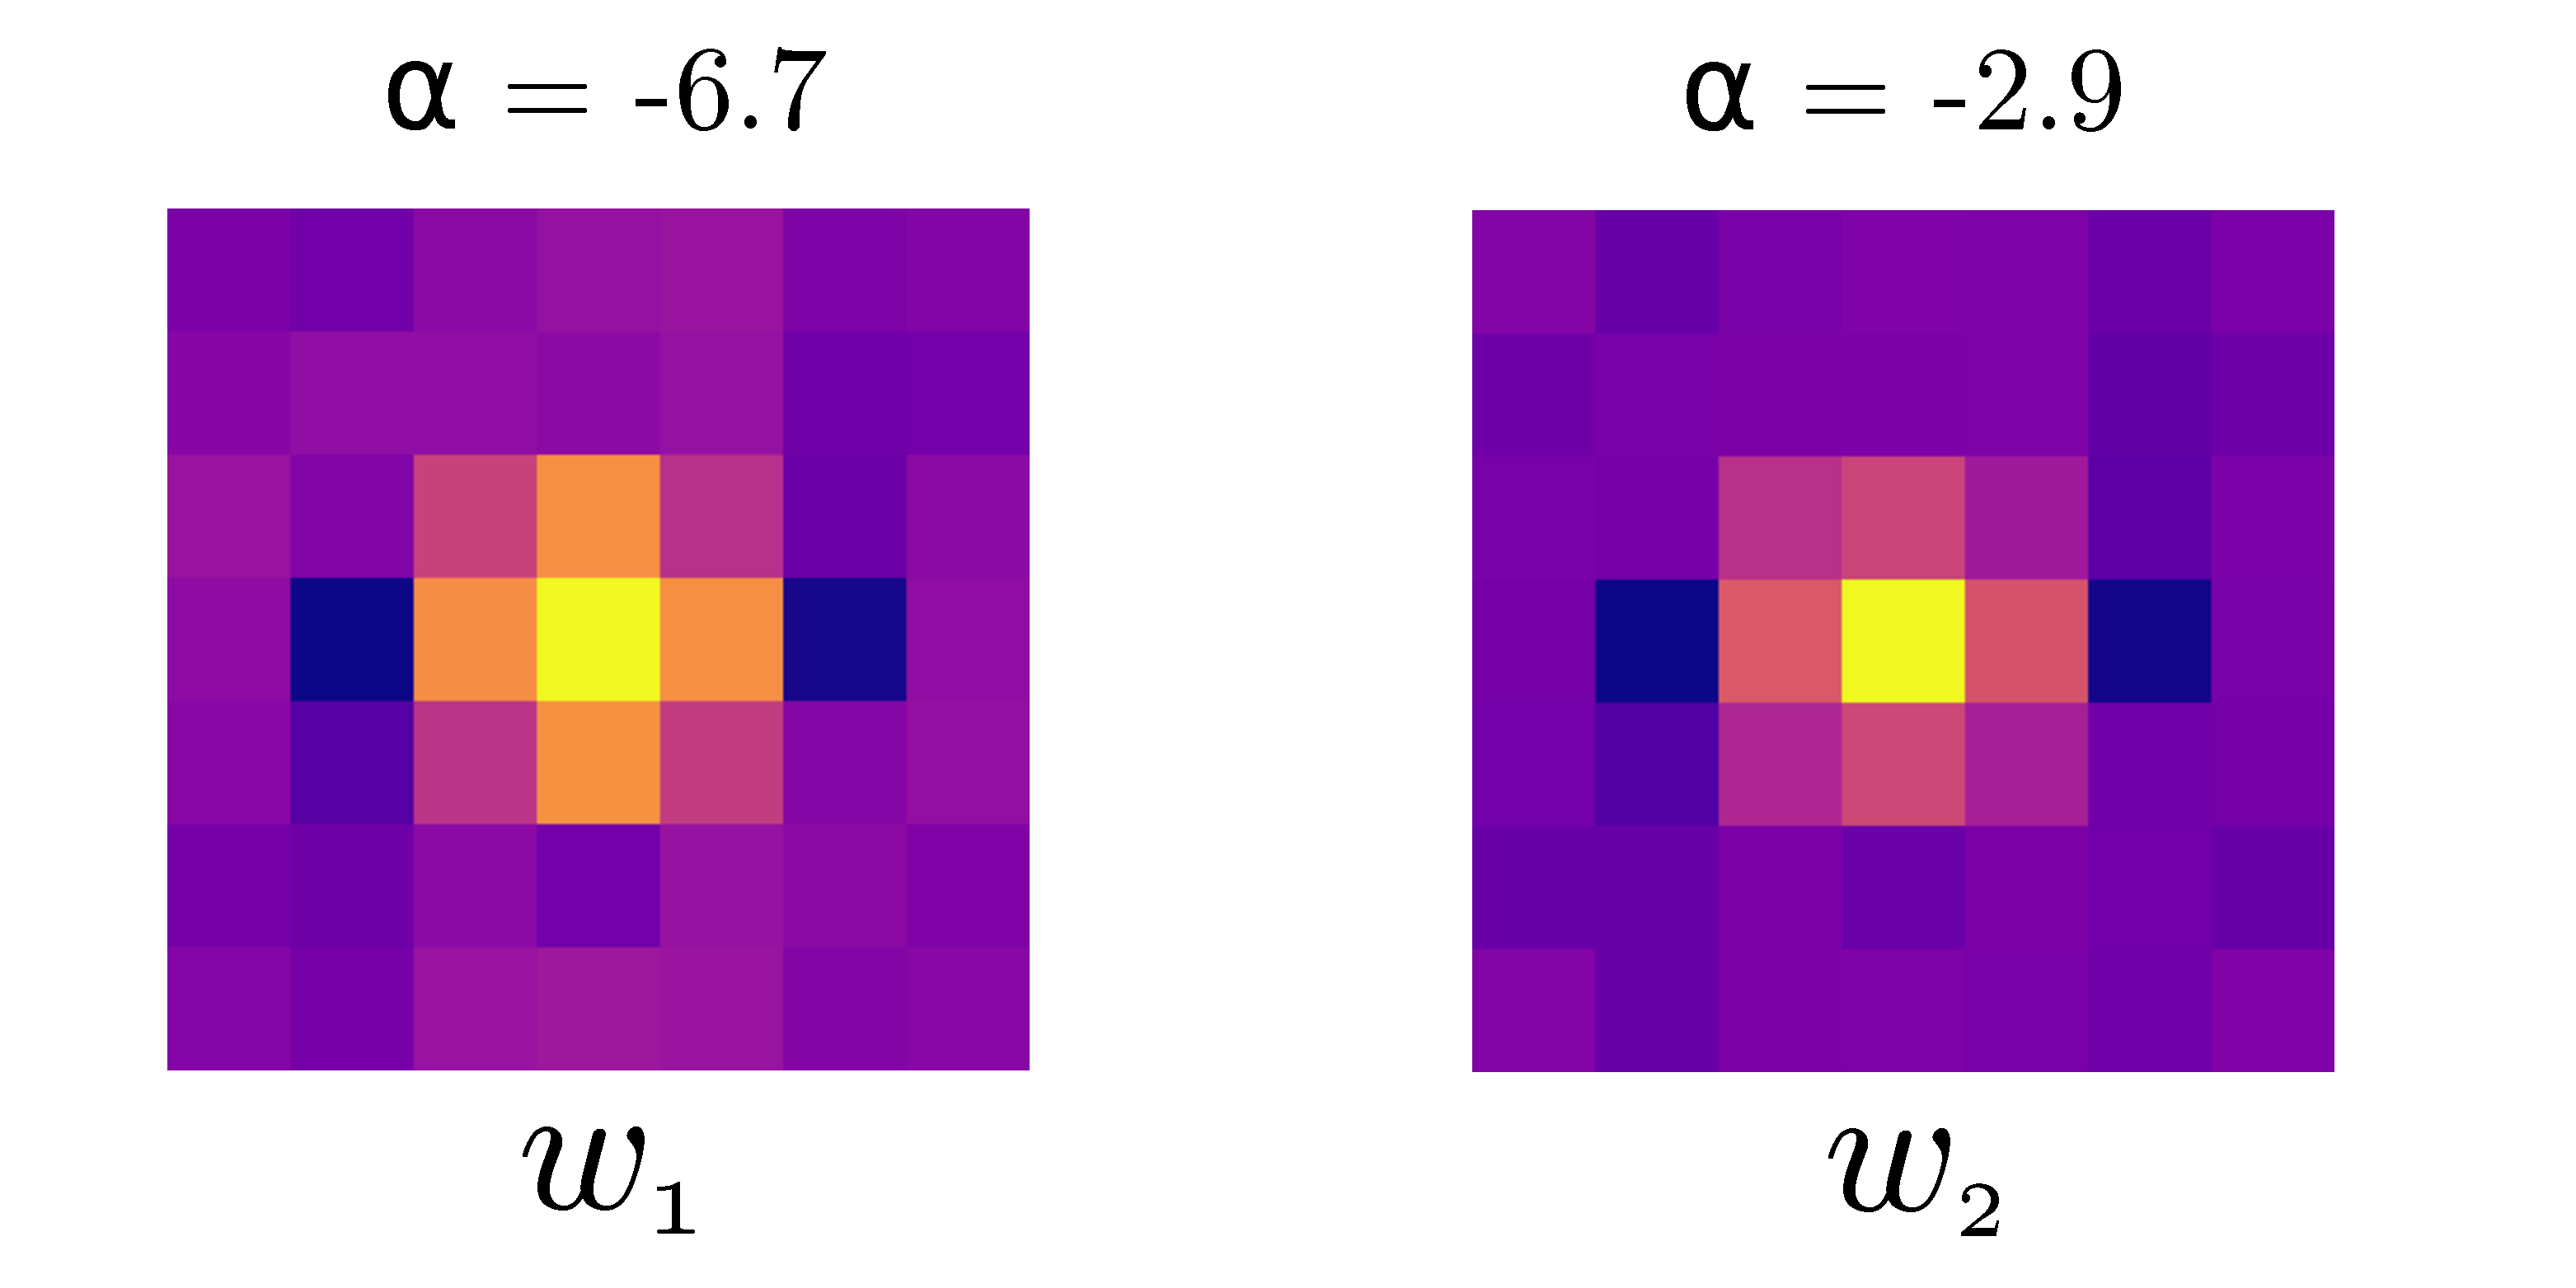
\includegraphics[width=0.36\linewidth]{parts/4-analyse_des_reseaux/deux_couches_pour_OPfondamentale/figures/square_fail.pdf}
    \vspace{1.0mm}
    \caption{ \centering État final du réseau $\mathcal{S}$MorphNetTanh à deux couches morphologiques, pour la fonction structurante cible carrée 3x3 et l'opération cible d'\textbf{érosion} sur la banque d'images d'entraînement MNIST, sans contrainte. Résultat : échec.}
    \label{fig:square_fail}
  \end{center}
\end{figure}

\vspace{-0.4mm}
On remarque que, pour cet exemple, le réseau a mal convergé, car la forme des noyaux est peu reconnaissable, les paramètres de contrôle $\alpha$ sont de très faible amplitude, et on obtient une valeur de perte sur les prédictions élevée, de l'ordre de $10^{-3}$. \\

\vspace{-1.0mm}
\noindent On peut cependant, pour cette structure carrée 3x3, tenter de la forcer à mieux converger, en lui imposant une contrainte dans la fonction de perte \textit{loss}. Dans notre cas, on prendra la contrainte sur la norme $L_1$, avec $l_c = 0$ (formule \ref{erreur_norm}). La convergence devient alors bien meilleure : on obtient l'état final des deux couches suivant, illustré fig. \ref{fig:square_success}.


\newpage

%figure
\begin{figure}[!htp]
  \begin{center}
    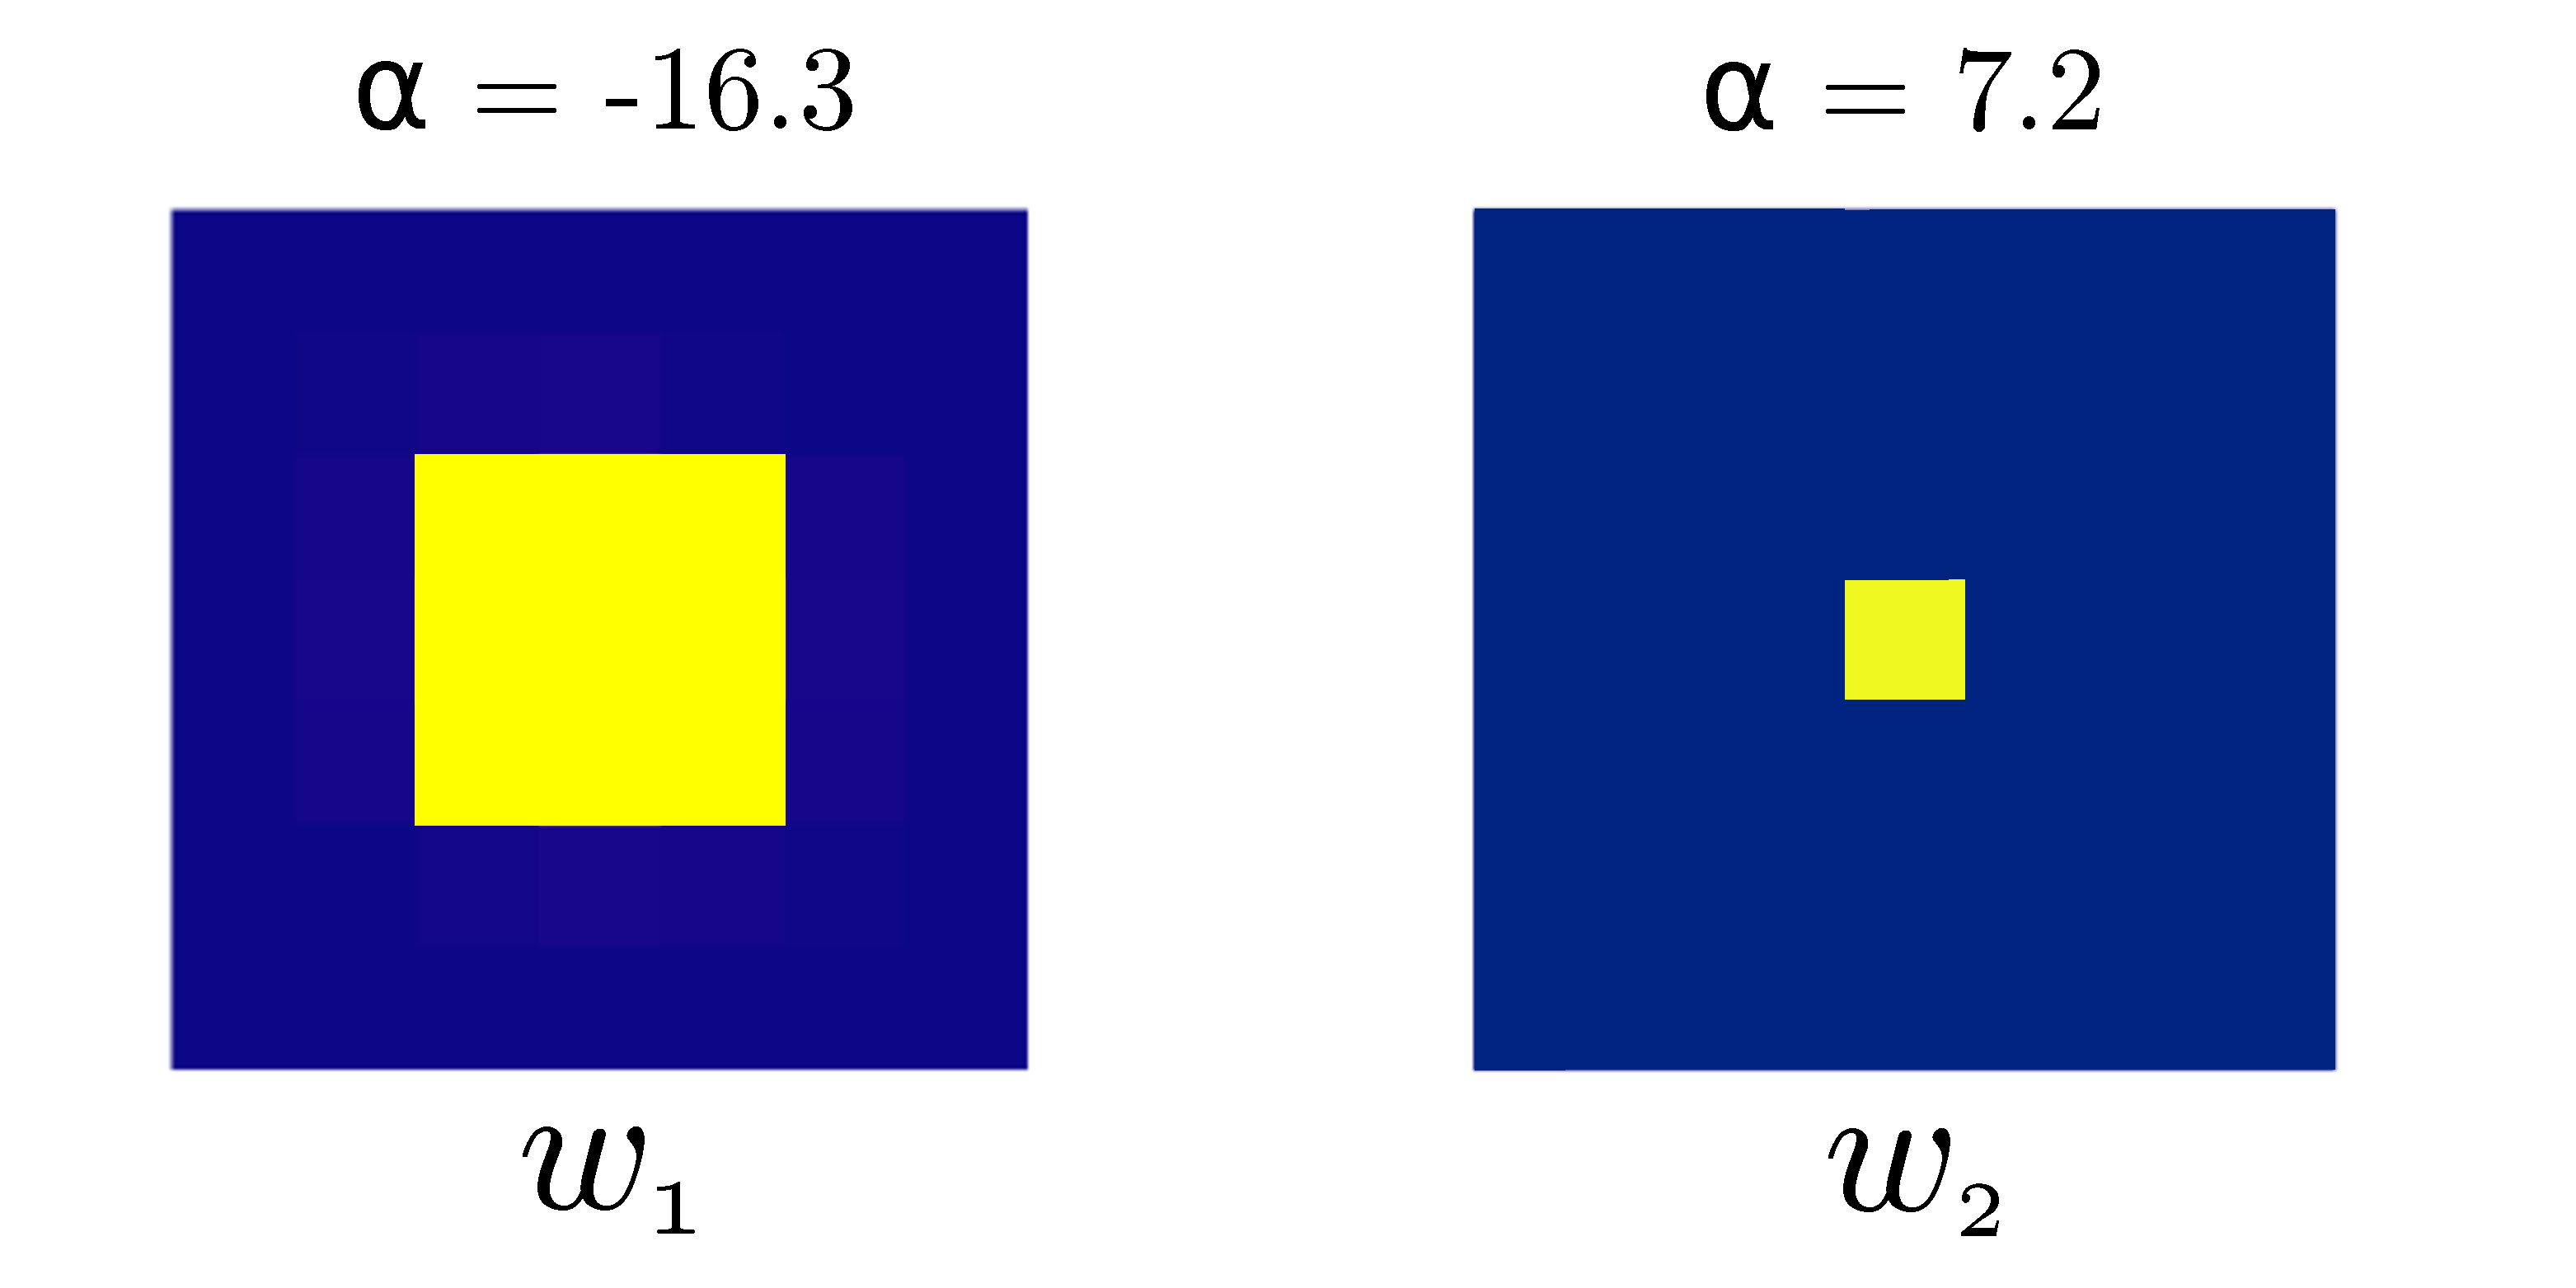
\includegraphics[width=0.36\linewidth]{parts/4-analyse_des_reseaux/deux_couches_pour_OPfondamentale/figures/square_success.pdf}
    \vspace{1.0mm}
    \caption{ \centering État final du réseau $\mathcal{S}$MorphNetTanh à deux couches morphologiques, pour la fonction structurante cible carrée 3x3 et l'opération cible d'\textbf{érosion} sur la banque MNIST, avec une contrainte des noyaux sur la norme $L_1$. Résultat : succès.}
    \label{fig:square_success}
  \end{center}
\end{figure}

\vspace{-0.2mm}
On remarque que, pour cet exemple encore, le réseau a, cette fois-ci, bien convergé, grâce à l'ajout de cette contrainte des noyaux $w$ sur la norme $l_1$ : la forme des noyaux est très reconnaissable (le premier noyau a la forme de la structure cible i.e. le carré 3x3, et le second a la forme de l'identité i.e. un unique pixel distinguable au centre du support), les paramètres de contrôle $\alpha$ ont une plus grande amplitude, et on obtient une valeur de perte sur les prédictions du réseau bien plus faible, de l'ordre de $10^{-6}$. \\

%\vspace{-0.0mm}
\noindent Parmi les deux groupes << succès >> et << échecs >> des résultats de convergence que l'on a distingués sur l'ensemble des expériences, en examinant uniquement les \textit{succès}, on peut remarquer que l'amplitude des paramètres $\alpha$ n'est jamais très élevée (de l'ordre de 10), et aussi, mais surtout, que l'on obtient \textit{toujours} la configuration des couches suivantes : la première couche a un noyau $w_1$ de la forme de la fonction structurante cible, avec un $\alpha$ associé négatif, et la seconde couche a un noyau $w_2$ de la forme de l'identité (un seul pixel actif), avec un $\alpha$ associé positif. On n'obtient jamais de composition originale ou plus complexe sur ces succès, même avec l'aide de contraintes pour favoriser certaines configurations, et on a toujours le même ordre : d'abord la structure cible, puis l'identité. C'est le cas par exemple du carré 3x3, aidé de la contrainte $L_1$, telle qu'illustrée figure \ref{fig:square_success} (d'abord carré 3x3, puis identité).

\vspace{3.6mm}

%\newpage

\subsubsection{Avec la dilatation}
\vspace{0.46cm}
On reprend ici, pour l'opération cible de dilatation, le même protocole d'expérimentation que pour l'érosion : on considère à nouveau un réseau $\mathcal{S}$MorphNetTanh qu'on munit de deux couches morphologiques, et on fixe ici l'opération cible à celle de la dilatation. On lance les différents entraînements du réseau avec l'ensemble des huit fonctions structurantes cibles considérées, avec en plus le carré binaire de taille 3x3, et ce toujours sur la banque MNIST. Tout comme pour l'érosion, on peut distinguer ici pour la dilatation deux groupes de résultats : les résultats à << succès >> de convergence, et ceux à << échec >> de convergence, tels que définis précédemment.


\newpage

\noindent Pour le carré 3x3 par exemple, à nouveau contraint par la norme $L_1$ (avec $l_c=0$) pour aider le réseau à converger correctement, on obtient l'état des deux couches morphologiques du réseau suivant, illustré figure \ref{fig:square_success_dilation} : \\

%figure
%\vspace{-1.4mm}
\begin{figure}[!htp]
  \begin{center}
    \includegraphics[width=0.36\linewidth]{parts/4-analyse_des_reseaux/deux_couches_pour_OPfondamentale/figures/square_success_dilation.pdf}
    \vspace{0.6mm}
    \caption{ \centering État final du réseau $\mathcal{S}$MorphNetTanh à deux couches morphologiques, pour la fonction structurante cible carrée 3x3 et l'opération cible de \textbf{dilatation} sur la banque MNIST, avec une contrainte des noyaux sur la norme $L_1$. Résultat : succès.}
    \label{fig:square_success_dilation}
  \end{center}
\end{figure}

\vspace{-2.0mm}
On peut à nouveau constater ici, dans le groupe des succès, l'uniformisation des solutions trouvées dans la décomposition de la fonction structurante cible par le réseau à deux couches. Sauf que, pour le cas de la dilatation, l'ordre entre structure cible et identité est inversée par rapport à celle de l'érosion : on a d'abord l'identité sur le noyau $w_1$ de la première couche, avec un $\alpha$ négatif, puis on a la forme de la structure cible sur le noyau $w_2$ de la seconde couche, avec un $\alpha$ positif. Pour l'exemple du carré 3x3, on a ainsi d'abord l'identité sur $w_1$, puis le carré 3x3 sur $w_2$ (fig. \ref{fig:square_success_dilation}). On remarque à nouveau que, d'une manière générale, l'amplitude des $\alpha$ reste faible.

\vspace{2.2mm}

%\newpage

\subsubsection{Discussion}
\vspace{0.32cm}
Dans le cas des expériences à succès, le réseau converge donc toujours vers la structure cible pour $w_1$ et l'identité pour $w_2$ avec l'\textit{érosion}, et, à l'inverse, vers l'identité pour $w_1$ et la structure cible pour $w_2$ avec la \textit{dilatation}. Ce constat, surprenant à priori, reste à ce jour inexpliqué. Il s'agit d'une configuration très solide, puisqu'il est difficile d'obtenir l'ordre inverse respectif des rôles entre les deux couches, malgré l'ajout de contraintes forçant cette inversion des rôles. Bien qu'elle soit théoriquement tout aussi valide que l'ordre initial, la seule manière qui a fonctionné dans notre étude pour inverser les rôles des deux couches, c'est avec une initialisation de ces dernières dans la configuration visée (forme des deux noyaux $w$ avec l'ordre inversé correspondant, et paramètres $\alpha$ du bon signe et légèrement éloignés de 0, de l'ordre de 0.1). \\

\vspace{-1.4mm}
\noindent L'ordre systématique entre structure cible et identité, selon l'érosion ou la dilatation, doit être lié aux propriétés de transformation de ces deux opérations sur les images d'entrée, et à l'ordre d'exécution des deux couches du réseau. La rétropropagation du gradient doit également jouer un rôle. Mais la cause de ce résultat reste inconnu.


%Parler de la multiplicité des possibilités, par décomposition exacte de l'opération, avec un élément structurant, en deux opérations avec deux éléments structurants. Evoquer le cas du carré 3x3 décomposable en un segment vertical de longueur 3 et un segment horizontal de longueur 3... \\

%Dire que ça dépend de l'ordre d'exécution entre les deux couches, ie entre identité et forme cible, et que ça doit être liée à la rétropropagation du gradient, mais qu'en n'en sait pas davantage, la question reste en suspens)\\

%Dire que c'est une configuration très solide, on n'arrive pas à avoir l'inverse, bien qu'elle soit théoriquement tout aussi valide. Même l'ajout de contraintes indépendantes sur les deux couches n'est pas suffisante. La seule manière dont on a réussi à inverser les rôles des deux couches, c'est avec l'initialisation dans la configuration visée (forme des deux noyaux, et paramètres $\alpha$ du bon signe et légèrement éloignés de 0, de l'ordre de 0.1). 

%%%%%%%%%%%%%%%%%%%%

%-> Dire que, dans les cas avec un succès de convergence (loss faible), on obtient toujours ... 
%   + illustration (évolution?)
%-> Dire qu'on obtient, sur beaucoup d'expériences, des échecs 
%   + illustration (évolution?)
%-> Dire que c'est une configuration très solide, on n'arrive pas à avoir l'inverse, bien qu'elle soit théoriquement tout aussi valide. Même l'ajout de contraintes indépendantes sur les deux couches n'est pas suffisante. La seule manière dont on a réussi à inverser les rôles des deux couches, c'est avec l'initialisation dans la configuration visée (forme des deux noyaux, et paramètres $\alpha$ du bon signe et légèrement éloignés de 0, de l'ordre de 0.1). 
%   + illustration (évolution?)
\newpage

% Impact de la banque d'images d'entraînement
\subsection{Impact du jeu de données d'entraînement}

\subsubsection{Description des banques MNIST et FashionMNIST}
\vspace{0.2cm}
Dans l'ensemble de ce rapport, jusqu'à maintenant, nous considérions tout particulièrement la banque d'images MNIST en tant que jeu de données d'entraînement des réseaux étudiés. Il s'agit d'un jeu composé de 70000 images digitales en niveaux de gris, échelonnées entre 0 et 1 et de taille 28x28 pixels, représentant des digits (chiffres) écrits à la main \cite{LeCun_2005}. Les objets sur les images (ensemble des pixels de valeurs strictement positives, qui se détache visuellement du fond de l'image, dont les valeurs sont proches de 0) de ce jeu de données sont particulièrement fins, et peuvent être considérés topologiquement comme des filaments entrelacés. Cet aspect-là rend ce jeu très spécifique dans le cadre d'opérations morphologiques, et peut donner sur les réseaux morphologiques étudiés des résultats bien particuliers. \\

\vspace{-1.2mm}
\noindent L'ensemble des expériences citées durant ce rapport a également été réalisé, en parallèle de MNIST, avec un autre jeu de données : FashionMNIST. Il s'agit d'une banque de 70000 images digitales en niveaux de gris, échelonnées entre 0 et 1 et de taille 28x28 pixels également, mais qui représente cette fois-ci des vêtements de tout type (pantalons, chemises, robes, etc.). Contrairement à MNIST, ce jeu de données représente donc des objets bien plus larges et imposants face au support des images, et les résultats d'entraînement des réseaux morphologiques avec un tel jeu peuvent être bien différents de ceux avec MNIST. \\

\vspace{-1.2mm}
\noindent La figure suivante (\ref{fig:mnist_and_fashionmnist}) permet de visualiser une partie des images des deux banques MNIST (\ref{fig:sum1}) et FashionMNIST (\ref{fig:sum2}). \\

%figure
\vspace{-0.2mm}
\begin{figure}[ht]
  \begin{center}
      \subfigure[MNIST]{
          \includegraphics[width=0.24\textwidth]{parts/4-analyse_des_reseaux/impact_database/figures/ill_mnist.pdf}
          \label{fig:sum1}}
      \hspace{12.0mm}
      \subfigure[FashionMNIST]{
          \includegraphics[width=0.24\linewidth]{parts/4-analyse_des_reseaux/impact_database/figures/ill_fashionmnist.pdf}
          \label{fig:sum2}}
    \vspace{-0.1mm}
    \caption{ \centering Echantillon des jeux de données MNIST (\ref{fig:sum1}) et FashionMNIST (\ref{fig:sum2}).}
    \label{fig:mnist_and_fashionmnist}
  \end{center}
\end{figure}

\vspace{-3.2mm}
Le but est alors de comparer les résultats de convergence d'un même réseau pour les même expériences entre ces deux jeux de données MNIST et FashionMNIST, et ainsi mieux comprendre leur impact sur la convergence des réseaux morphologiques.

\newpage

\subsubsection{Différences de résultats entre les jeux}
\vspace{0.2cm}
On souhaite comparer les résultats de convergence de réseaux entraînés sur MNIST avec ceux entraînés sur FashionMNIST pour les mêmes expériences, dans le but d'en tirer des caractéristiques et une différence globale de comportement des réseaux liés à ces deux jeux de données. Prenons par exemple le réseau $\mathcal{S}$MorphNetTanh composé de deux couches morphologiques, et que l'on munit simplement d'un partage de poids doux (contrainte entre $w_1$ et $w_2$ dans la \textit{loss}, eq. \ref{MSEpConstraintFilters}). On fait alors une analyse rapide en constatant uniquement la forme des noyaux du réseau dans son état final, moyennée sur 6 runs par expérience. On obtient les résultats représentés sur la figure \ref{fig:results_mnist_vs_fashionmnist}, avec MNIST à gauche (\ref{fig:suk1}) et FashionMNIST à droite (\ref{fig:suk2}). \\

%figure
\vspace{0.2mm}
\begin{figure}[ht]
  \begin{center}
      \subfigure[Avec MNIST]{
          \includegraphics[width=0.47\textwidth]{parts/4-analyse_des_reseaux/impact_database/figures/ft1.pdf}
          \label{fig:suk1}}
      \hspace{1.6mm}
      \subfigure[Avec FashionMNIST]{
          \includegraphics[width=0.47\linewidth]{parts/4-analyse_des_reseaux/impact_database/figures/ft2.pdf}
          \label{fig:suk2}}
    \caption{ \centering Noyaux $w$ associés par paires du réseau $\mathcal{S}$MorphNetTanh après convergence, entraîné sur les jeux de données MNIST (\ref{fig:suk1}) et FashionMNIST (\ref{fig:suk2}). Les cases à gauche et à droite de même emplacement correspondent à la même expérience.}
    \label{fig:results_mnist_vs_fashionmnist}
  \end{center}
\end{figure}

\vspace{-2.4mm}
Les différences de résultats des noyaux $w$ pour ces expériences-là entre les deux jeux MNIST et FashionMNIST sont très notables. Certains résultats semblent meilleurs avec la banque FashionMNIST, comme ceux avec les structures cibles \textit{adiag} pour l'ouverture (troisième ligne [milieu bas] première paire [tout à gauche]) ou \textit{disk2} (deuxième ligne troisième paire, et dernière ligne troisième paire), tandis que d'autres semblent meilleurs avec FashionMNIST, comme ceux avec les structures cibles \textit{brand} (première ligne deuxième paire, et troisième ligne deuxième paire) ou \textit{complex} pour la fermeture (première ligne troisième paire). Les résultats sont très diversifiés, et ne plaident pas significativement en la faveur d'un des deux jeux de données. \\

\vspace{-1.0mm}
\noindent Les mêmes observations et la même conclusion peuvent être faites avec les autres réseaux morphologiques ($p$ConvNet, $\mathcal{L}$MorphNet et $\mathcal{S}$MorphNet) et dans les autres configurations de réseaux (avec/sans partage de poids, avec/sans contrainte géométrique sur $w$ ou sur $\alpha / p$, initialisation aléatoire / initialisation gaussienne, etc.).


\newpage

Plusieurs hypothèses peuvent expliquer ces différences de résultats entre les deux jeux de données. 
En particulier, l'aspect << fin >> des objets sur les images MNIST doit impacter l'entraînement des réseaux de manière différente que ne le font les aspects << épais >> et << étendu >> des objets sur les images FashionMNIST.
Les objets fins sur les images peuvent par exemple s'effacer intégralement avec une petite opération d'\textit{érosion}, et donc la prédiction sur l'érosion serait moins facile à faire pour les réseaux morphologiques ciblant cette opération ou bien ciblant l'ouverture (qui commence par une érosion, et donc peut directement effacer les objets avant même la dilatation). \\

\vspace{-1.6mm}
\noindent C'est en effet ce que l'on observe sur la figure \ref{fig:results_mnist_vs_fashionmnist} : on constate avec MNIST (\ref{fig:suk1}) que ce sont les résultats sur la fermeture (moitié supérieure) qui semblent plus précis que ceux sur l'ouverture (moitié inférieure), notamment en observant les structures \textit{adiag} et \textit{complex}. Avec FashionMNIST (\ref{fig:suk2}), on constate l'inverse : ce sont les résultats sur l'ouverture (dessous) qui semblent plus précis que ceux sur la fermeture (dessus). Cela peut s'expliquer par la trop petite place laissée au fond de l'image sur son support, à cause de l'épaisseur des objets, et donc par le fait qu'une dilatation (et donc une fermeture) supprimerait une trop grande partie du fond, ce qui rendrait les prédictions sur la dilatation et la fermeture avec FashionMNIST plus délicates.

\vspace{1.0mm}

%%%

%-> Les différences sont notables (certains mieux, d'autres pires)
%-> C'est la même conclusion avec les autres réseaux et les autres configuration de réseaux (avec/sans contrainte, avec/sans partage de poids, avec/sans initialisation gaussienne, etc.)

%%%-> Dire que sur MNIST (avec images en positif), on aurait plutôt dit que c'est l'érosion qui poserait problème, car les éléments sont très fins et s'effacent quasiment intégralement avec une petite érosion, donc que la prédiction sur l'érosion serait moins facile à faire... Mais on observe l'inverse ! Warum ??? <=== !!!NON!!!, pas pour l'exemple choisi ! Par contre, avec une initialisation gaussienne par exemple, oui en effet...
%\newpage

\subsubsection{Résultats avec les jeux en négatif}
\vspace{0.3cm}
On considère ici les images des banques MNIST et FashionMNIST en \textit{négatif}, c'est-à-dire qu'on leur applique : $f \mapsto 1-f$. Ainsi, les propriétés de chacune de ces deux banques d'images sont inversées : les images de MNIST en négatif comportent des objets (parties du support dont la valeur est proche de 1) très épais qui s'étalent le long des quatre bords du support et occupent une grande partie de l'espace sur ce dernier, englobant un fond (parties du support de valeur proche de 0) filamentaire fin et centré sur le support, qui disparaît facilement avec une dilatation ; tandis que les images de FashionMNIST en négatif comportent plutôt des objets qui s'étalent également le long des bords, mais qui, à l'inverse de MNIST, sont fins et disparaissent facilement avec une érosion, et qui entourent un fond épais centré sur le support. \\

\vspace{-1.6mm}
\noindent En relançant les mêmes entraînements que précédemment sur $\mathcal{S}$MorphNetTanh à deux couches morphologiques muni d'un partage de poids doux, mais avec cette fois-ci les deux jeux de données MNIST et FashionMNIST en négatif, on obtient les conclusions inverses par rapport à celles liées aux images en positif : sur MNIST, les résultats de convergence du réseau sont ici globalement meilleurs avec l'opération cible d'ouverture qu'avec la fermeture, et sur FashionMNIST, à l'inverse, les résultats sont globalement meilleurs pour la fermeture que pour l'ouverture (ce dernier cas présentant les mêmes défauts et irrégularités dans la forme des noyaux $w$ que pour les résultats de fermeture avec les images en positif). Ce qui est cohérent avec les caractéristiques inversées des images négatives par rapport aux images positives.
%(décrites ci-dessus) 

%%%

%-> Parler des expériences faites en négatif (là, c'est l'érosion qui est effectivement moins bonne que la dilatation ... l'efficacité entre les différentes opérations sont inversées, ce qui est cohérent, car les éléments sur les banques d'images sont inversés en négatifs. Si on peut faire la distinction entre un élément sur une image et le support (fond) de l'image, eh bien les images en positif avec de petits éléments deviennent, en négatif, des images avec de gros éléments et de petits trous.)
%Dire aussi qu'on obtient, avec les images d'entraînement en négatif, les résultats de performance inverses entre ouverture et fermeture (et entre érosion et dilatation)!!!
\newpage

% Relation entre complexité de la structure cible et échecs de convergence
\subsection{Relation entre complexité et échec de convergence}

\subsubsection{Complexité de la forme de la fonction structurante cible}
\vspace{0.2cm}
Dans leur article, Hermary et al. \cite{Hermary_2022}, pour tenter de donner une explication aux différents échecs de convergence de leurs expériences, émettaient l'hypothèse que le fait qu'un élément (ou fonction) structurant << touche >> le bord de son support (i.e. le fait qu'il existe un pixel au bord du support de valeur strictement supérieure à 0 pouvant être associée à l'objet de l'image) aide le réseau, lors de son entraînement, à converger de manière plus précise et certaine vers l'élément structurant cible. \\

\vspace{-1.6mm}
\noindent En reproduisant les différentes expériences de leur article, avec notamment leurs six fonctions structurantes cibles telles que décrites dans les grandes parties précédentes (\textit{cross3}, \textit{cross7}, \textit{disk2}, \textit{disk3}, \textit{diamond3} et \textit{complex}), on peut effectivement constater que les cas d'échec interviennent uniquement sur les structures dont aucune partie ne touche le bord de leur support (\textit{cross3} et \textit{disk2}), là où les structures touchant le bord de leur support donnent systématiquement lieu à un succès de convergence (\textit{cross7}, \textit{disk3}, \textit{diamond3} et \textit{complex}), du moins pour ces fonctions structurantes-là (fig. \ref{fig:art_resultats_opening} et \ref{fig:art_resultats_closing}). \\

\vspace{-1.6mm}
\noindent Une explication donnée est le fait que, lors de la rétropropagation du grandient pendant l'apprentissage du réseau, ce sont les poids des bords du support des noyaux $w$ qui semblent se mettre à jour en premier, ou du moins qui convergent plus rapidement. Par exemple, sur la figure \ref{fig:c_awayOPP} montrant l'évolution des deux noyaux du réseau pour la fonction structurante cible \textit{adiag}, avec ou sans contrainte $C_\text{awayOPP}$, on voit lors des premières époques que ce sont effectivement les poids au bord du support qui semblent converger en premier vers leur état final : les coins supérieur gauche et inférieur droit, par lesquels passe la diagonale, prennent en premier les plus grandes valeurs, et les coins supérieur droit et inférieur gauche prennent de plus petites valeurs, là où le centre du support reste creux et surtout très homogène. La forme de la structure semble se dessiner en partant des bords jusqu'au centre du support. \\

\vspace{-1.0mm}
Cependant, avec les deux autres fonctions structurantes créées en plus (\textit{adiag} et \textit{brand}), on remarque que cette propriété n'est ici pas respectée : malgré le fait que \textit{adiag} touche largement les bords d'une part et d'autre de son support, les réseaux $\mathcal{S}$MorphNet et $\mathcal{S}$MorphNetTanh, sans contrainte, ont tous deux du mal à converger vers cette forme diagonale, pour laquelle les métriques de performances des réseaux sont moyennes voire mauvaises (de l'ordre de $10^-3$ pour la \textit{loss}). À l'inverse, pour la fonction structurante \textit{brand}, les deux réseaux arrivent très bien à trouver la forme de la structure cible, malgré le fait que cette dernière ne touche pas le bord (fig. \ref{fig:SMvsSMTH_opening_mnist} et \ref{fig:SMvsSMTH_closing_mnist}). \\

\vspace{-1.6mm}
\noindent Des expériences complémentaires ont été réalisées en ajoutant, dans \textit{brand}, un unique pixel au bord du support. Et les résultats de convergence des réseaux avec cette structure cible-là, qui touche donc le bord, sont même légèrement moins bons que ceux avec la structure \textit{brand} originelle, comme le montre la figure \ref{fig:touch_notouch_borders} ci-après.


\newpage

%figure
%\vspace{-0.8mm}
\begin{figure}[htp]
  \begin{center}
    \includegraphics[width=1.00\linewidth]{parts/4-analyse_des_reseaux/complexity_and_fails/figures/z_touchnotouch.pdf}
    \vspace{-4.0mm}
    \caption{ \centering Évolution de la forme des deux noyaux du réseau et de leur \textit{RMSE} en fonction de la progression de l'entraînement (en \% avant l'état final), pour la fermeture sur MNIST, avec le \textit{brand} (haut) et le \textit{brand} avec un pixel en plus au bord (bas).}
    \label{fig:touch_notouch_borders}
  \end{center}
\end{figure}

\vspace{-3.0mm}
L'hypothèse que la structure cible touche (resp. ne touche pas) le bord de son support puisse déterminer le succès (resp. l'échec) de convergence du réseau ne peut donc pas, à elle seule, expliquer l'ensemble des échecs de convergence. En revanche, en exploitant les résultats de convergence de diverses expériences, avec davantage de formes différentes de fonctions structurantes cibles, il semble se dessiner un lien - une correlation positive - entre une certaine << complexité >> de la forme de la structure cible et la réussite du réseau dans sa convergence. En effet, plus la forme de la structure cible semble << complexe >>, plus le réseau semble converger de manière précise et juste, avec des noyaux $w$ de forme davantage proche de celle de la structure cible. \\

\vspace{-2.0mm}
\noindent Cette notion de << complexité >> des fonctions structurantes cibles reste très subjective et mal définie. Elle prend en compte à la fois la \textit{taille} de la structure par rapport à son support (si elle est plus petite, alors les configurations à deux couches où elle est symétriquement translatée sont strictement équivalentes), la multiplicité des \textit{nuances de gris} dont l'élément est composé, et les \textit{caractéristiques topologiques} de cette structure (rotondité, connexité, convexité, extrémités...). Ce premier aspect (élément plus petit que le support) peut expliquer les échecs des cas où l'élément <<ne touche pas le bord>>. \\
%blablabla + impact de la taille du support : plus de variables ! Donc plus de configurations possibles, et plus de minima locaux dans la \textit{loss} \\

\vspace{-2.0mm}
\noindent Cette notion de << complexité >> d'une structure morphologique serait inversement correlée au nombre de décompositions exactes possibles de cet élément dans le cadre d'une érosion ou d'une dilatation. Par exemple, le carré 3x3 peut être considéré comme << peu complexe >>, car il existe une multitude de décompositions de cette structure, par exemple celle en deux segments successifs de longeur 3 (et de largeur 1), l'un horizontal et l'autre vertical, dans le cadre d'une érosion ou d'une dilatation. C'est une explication fort probable des nombreux échecs de convergence des réseaux à deux couches avec comme structure cible le carré 3x3 sur un support de taille 7x7 (en plus de la taille du support qui multiplie les configurations possibles).


\newpage

Une explication possible à cette correlation positive entre complexité de la forme de la structure cible et succès de convergence des réseaux, est le fait que plus la structure est complexe, plus elle est << unique >> : il existerait moins de formes différentes possibles << proches >> morphologiquement parlant de cette structure, et moins de décompositions possibles de cet élément en plusieurs sous-éléments distincts (dans le cadre de réseaux multi-couches). Cette diminution du nombre de formes théoriques possibles << proches >> de la structure visée équivaut à une diminution du nombre de minima locaux possibles dans la fonction de perte \textit{loss} qui sont << proches >> du minimum global associé à la structure cible. Ce qui ferait ainsi que les noyaux $w$ du réseau arrivent mieux à converger vers cette structure cible, et avec plus de précision et de rapidité, car il y aurait moins de minima locaux proches de ce minimum global visé. À l'inverse, une structure cible trop << élémentaire >> impliquerait une multiplicité des solutions locales possibles (i.e. minima locaux dans la \textit{loss}), et donc amènerait davantage le réseau à converger vers l'un de ces minima locaux (un mauvais résultat). \\

\vspace{-1.6mm}
\noindent Ces explications restent néanmoins au stade d'hypothèses, qui doivent être vérifiées et validées. La notion de << complexité >> d'une forme reste également très subjective, et une définition précise de ce terme doit être formulée. Son rôle dans les succès ou les échecs de convergence des réseaux pourrait alors être évalué et quantifié.


\vspace{1.0mm}


%Parler de la relation entre "complexité de la forme du noyau" et multiplicité des solutions locales possibles (minima locaux dans la loss) et mauvaise convergence des réseaux... 
%+ Parler de la définition très vague de la notion de "complexité" des formes : comment savoir si une forme est plus << complexe >> qu'une autre ? Réponse proposée : le nombre de décompositions possibles de cet élément dans le cadre d'une érosion ou dilatation. \\

%%%-> Parler de l'impact de la complexité de la forme des noyaux ("complexité" + parler de si il touche le bord ou non [7], qui n'est pas non plus une hypothèse qui suffit seule à elle-même car il y a des cas où si l'élément structurant touche le bord en ajoutant un seul pixel, alors la convergence est moins bonne que sans ce dernier pixel)! Prendre l'exemple du carré 3x3... (+ impact de la taille du support : plus de variables ! Donc plus de configurations possibles, et plus de minima locaux dans la \textit{loss})
%\newpage

\subsubsection{Complexité de la configuration du réseau}
\vspace{0.3cm}
En plus de la corrélation positive établie entre << complexité >> de la fonction structurante cible et succès de convergence du réseau, il semble y avoir également corrélation, mais cette fois-ci négative, entre ces succès et une certaine << complexité >> dans la \textit{configuration} du réseau : son architecture, le nombre de couches morphologiques, la taille des noyaux des couches, ou plus généralement l'ensemble des hyperparamètres du réseau. 
Cette notion de << complexité >> de la configuration d'un réseau peut se traduire en particulier par la taille et la densité de ce dernier : un réseau morphologique devient davantage << complexe >> si la \textit{taille du support} de ses noyaux $w$ augmente ou si le \textit{nombre de couches} morphologiques successives qu'il contient augmente, donc de manière générale si le nombre de poids apprenables par le réseau augmente. \\

\vspace{-1.6mm}
\noindent Cette corrélation peut s'expliquer simplement : plus le réseau est grand et dense, plus il existe de configurations possibles du réseau, et donc plus il y aura de minima locaux dans la fonction de perte \textit{loss} vers lesquels le réseau risque de converger. Les configurations possibles du réseau pour des caractéristiques ciblées (comme la forme des noyaux $w$) étant moins nombreuses avec des petits réseaux peu complexes qu'avec de grands réseaux denses. 
Mais ces explications restent encore une fois des hypothèses, qui doivent être vérifiées. Il doit encore exister une multitude de caractéristiques sur les réseaux ou sur les éléments cibles pouvant avoir un rôle concret dans les succès ou les échecs de convergence des réseaux, car ce problème reste sous-déterminé.


%Parler de la relation entre "complexité de la forme du noyau" et multiplicité des solutions locales possibles (minima locaux dans la loss) et mauvaise convergence des réseaux... \\

%-> Parler de l'impact du nombre de couches morphologiques successifs (+ il y en a, + l'état final du réseau après convergence est "random" ou loin de ce que l'on visait, car il y a plus de variables, donc davantage de configurations possibles, donc des minima locaux dans la \textit{loss} plus nombreux et prononcés) 
%+ D'une manière générale, le nombre d'éléments (poids) apprenables dans le réseau et par le réseau ( + la taille du support des noyaux joue donc également, car il y a plus de poids variables à apprendre, donc plus de configurations possibles)...
\newpage

% Autres...
\subsection{Autres rapides analyses}

\subsubsection{Importance des $\alpha$ dans la convergence des réseaux}
\vspace{0.2cm}
Lors des différentes expériences effectuées, notamment sur les cas d'échec de convergence, une observation à priori étonnante a pu être faite sur l'impact de la valeur des paramètres de contrôle $\alpha$ (ou $p$), notamment celui de leur signe, sur la direction dans laquelle converge le réseau lors de son entraînement. Les couches morphologiques, en particulier $\mathcal{S}$Morph et $\mathcal{S}$MorphTanh, se comportent en effet comme des moyenneurs quand leur paramètre de contrôle $\alpha$ est proche de 0, peu importe son signe. On pouvait alors espérer que la différence de comportement d'un réseau, dont le paramètre $\alpha$ d'une couche est proche de 0, serait minime voire négligeable entre un $\alpha$ positif et un $\alpha$ négatif. Or, plusieurs expériences permettent de montrer que le signe des paramètres $\alpha$, même très proches de 0, a un impact majeur, voire plus important que la forme des noyaux $w$, sur la direction de convergence des réseaux. \\

%figure
\vspace{-0.6mm}
\begin{figure}[htp]
  \begin{center}
    \includegraphics[width=1.00\linewidth]{parts/4-analyse_des_reseaux/others/figures/zzzzz.pdf}
    \vspace{-4.0mm}
    \caption{ \centering Évolution de la forme des deux noyaux $w$ du réseau $\mathcal{S}$MorphNetTanh et de leur \textit{RMSE} en fonction de la progression de l'entraînement (en \% avant l'état final), pour l'ouverture sur MNIST avec le \textit{disk2}, sur trois types d'initialisation.}
    \label{fig:zzzzz}
  \end{center}
\end{figure}

\vspace{-2.0mm}
%La figure \ref{fig:zzzzz} ci-dessus montre en effet, sur un cas où le réseau $\mathcal{S}$MorphNetTanh à deux couches sans contrainte, avec l'opération cible d'ouverture et la structure cible \textit{disk2} sur MNIST, converge initialement vers un échec (tiers haut), que ce même réseau, en initialisant ses noyaux avec la structure cible exacte, converge exactement vers le même état d'échec (tiers milieu), mais que ce réseau encore, avec cette fois uniquement une initialisation des paramètres de contrôle $\alpha$ de très faible amplitude (0.1) mais du signe recherché, converge effectivement bien vers l'état cible de succès (tiers bas).
La figure \ref{fig:zzzzz} ci-dessus illustre le cas du réseau $\mathcal{S}$MorphNetTanh à deux couches morphologiques - muni d'aucune contrainte sur ces dernières ni d'aucun partage de poids, dont l'opération cible est l'ouverture et la structure cible est le \textit{disk2}, et entraîné sur MNIST -, qui converge initialement vers un échec (tiers supérieur de la figure).

\newpage

\noindent Ce même réseau, en initialisant ses deux noyaux par la structure cible exacte recherchée, converge exactement vers le même état d'échec (tiers central). Cependant, ce même réseau encore, avec cette fois uniquement une initialisation des paramètres de contrôle $\alpha$ de très faible amplitude ($|\alpha| = 0.1$) mais du signe recherché (négatif pour $\alpha_1$ et positif pour $\alpha_2$, comme on est dans le cadre d'une opération cible d'ouverture), converge effectivement bien vers l'état cible de succès (tiers inférieur). \\

\vspace{-1.6mm}
%\noindent 
Cela montre que le déplacement des paramètres de contrôle $\alpha$, même de très faible amplitude, vers leur signe cible respectif, a un impact bien plus important sur la réussite de la convergence que ne l'a le déplacement des poids des noyaux vers la forme exacte de la structure cible. Cette même conclusion peut être faite sur d'autres expériences encore qui sont initialement des échecs, et dont le signe des $\alpha$ dans leur état final n'est pas le bon recherché. Une bonne valeur (à l'initialisation ou au cours de l'entraînement) des paramètres de contrôle $\alpha$, et en particulier le bon signe de ces paramètres, a donc une importance majeure, probablement supérieure à celle de la forme des noyaux $w$, dans le succès de la convergence des réseaux.

\vspace{1.0mm}


%Importance des paramètres de contrôle $\alpha$ des couches morphologiques dans la convergence des réseaux
%+ Parler de l'impact des alphas sur la convergence des réseaux : pour certains échecs où les deux $\alpha$ finissent par être proches de 0 et du même signe, l'initialisation des noyaux $w$ en la forme cible n'est même pas suffisante pour que le réseau converge bien. Par contre, l'initialisation des $\alpha$ avec le bon signe pour chacun et une très faible amplitude, tout en gardant une forme aléatoire pour l'initalisation des $w$, permet quant à elle de faire converger le réseau corresctement.

%\newpage

\subsubsection{Application au débruitage}
\vspace{0.3cm}
Dans l'ensemble des travaux entrepris dans le cadre de ce stage, nous nous sommes intéressés en particulier à l'aspect théorique des couches morphologiques et des réseaux associées, et à l'amélioration et l'analyse comportementales de ces réseaux de neurones, sans vraiment nous pencher sur leur côté applicatif. Cette dernière partie est donc dédiée à une analyse rapide des résultats de l'une des applications pratiques possibles de tels réseaux morphologiques. Ces applications sont nombreuses, en particulier en traitement d'images. L'une d'elles est classiquement le débruitage. \\

\vspace{-1.0mm}
\noindent Dans le cadre de l'application pratique classique de débruitage poivre-et-sel d'images par un réseau de neurones morphologique, on considère un réseau $\mathcal{S}$MorphNetTanh, que l'on munit de quatre couches morphologiques $\mathcal{S}$MorphTanh. Cela afin que le réseau puisse simuler successivement les opérations d'ouverture et de fermeture, ou inversement : il faut donc deux couches simulant une érosion, et deux autres simulant une dilatation, toutes quatre disposées en rimes embrassées. On entraîne alors le réseau construit avec uniquement un ensemble d'images en entrée du réseau (input), sur lesquelles on aura ajouté au préalable le bruit poivre et sel (avec une certaine proportion surfacique d'occupation du bruit), ansi qu'avec l'ensemble des images cibles correspondantes visées par le réseau, qui sont les images d'origine avant l'ajout manuel du bruit. Il n'y a donc ici pas d'élément structurant cible, ni vraiment d'opération morphologique cible, bien qu'on espère que le réseau simule la succession d'une ouverture et d'une fermeture. On prendra ici le jeu d'entraînement FashionMNIST. \\

\vspace{-1.0mm}
\noindent Un exemple des résultats de débruitage du réseau entraîné est présenté figure \ref{fig:debruitage}.


\newpage

%figure
%\vspace{-0.6mm}
\begin{figure}[htp]
  \begin{center}
    \includegraphics[width=0.90\linewidth]{parts/4-analyse_des_reseaux/others/figures/shoes_data.pdf}
    \vspace{1.2mm}
    \caption{ \centering Résultats de débruitage d'une image représentant une chaussure par le réseau $\mathcal{S}$MorphNetTanh à quatre couches entraîné sur FashionMNIST, avec plusieurs niveaux de bruit poivre et sel (en proportion de surface occupée).}
    \label{fig:debruitage}
  \end{center}
\end{figure}

\vspace{-0.8mm}
Malgré des valeurs de \textit{loss} plutôt élevées de l'ordre de $10^{-3}$ à $10^{-2}$, les résultats visuels de débruitage du réseau semblent plutôt bons à l'oeil nu : le réseau retrouve toujours globalement la forme de la chaussure, même à très haute proportion de bruit, et les pixels poivre et sel disparaissent très bien de l'image bruitée, même à 50\%. Une opération morphologique à la main ne pourrait faire que légèrement mieux. \\

\vspace{-1.0mm}
\noindent Cependant, bien que les résultats de débruitage semblent << plutôt bons >>, l'état du réseau l'est bien moins, car la forme des noyaux $w$ est très aléatoire et manque de régularité, et, surtout, les paramètres de contrôle $\alpha$ sont toujours très proches de 0. \\

%figure
%\vspace{-0.4mm}
\begin{figure}[htp]
  \begin{center}
    \includegraphics[width=0.80\linewidth]{parts/4-analyse_des_reseaux/others/figures/aaaaa.pdf}
    \vspace{-1.6mm}
    \caption{ \centering Noyaux $w$ et paramètres de contrôle $\alpha$ des quatre couches du réseau $\mathcal{S}$MorphNetTanh après entraînement sur FashionMNIST bruitée à 10\%.}
    \label{fig:aaaaa}
  \end{center}
\end{figure}

\vspace{-2.6mm}
La figure \ref{fig:aaaaa} ci-dessus présente l'état des quatre couches du réseau après un entraînement sur les images de la banque FashionMNIST bruitées à 10\%. D'après l'ordre des signes des $\alpha$, on peut en déduire que le réseau a le comportement d'une pseudo-fermeture suivie d'une pseudo-ouverture, ce que l'on visait initalement. Mais les $\alpha$ restent très proches de 0. On remarque sur les autres proportions de bruitage que plus cette proportion est élevée, plus les $\alpha$ sont proches de 0, et donc plus les couches ont le comportement d'un moyenneur, ce qui peut être observé sur la figure \ref{fig:debruitage}.

\newpage

%========================================================================================
%	5. CONCLUSION
%========================================================================================

\section{Conclusion}
\vspace{0.2cm}
Les travaux menés dans le cadre de ce projet << Réseaux de neurones morphologiques >> sont multiples et variés. Ils ont abouti à différents résultats pour l'amélioration de la convergence de ces réseaux, ainsi qu'à des analyses de leurs propriétés sur diverses aspects. Dans la continuité des constats de l'état de l'art, notamment ceux de Kirszenberg et al. \cite{Kirszenberg_2021} et de Hermary et al. \cite{Hermary_2022}, c'est le réseau $\mathcal{S}$MorphNet, plus efficace que les autres de la littérature, qui a été en particulier étudié pour ce projet. \\

\vspace{-1.0mm}
\noindent Ce réseau $\mathcal{S}$MorphNet converge, lors de son entraînement, avec une haute précision et une grande rapidité, notamment dans le cadre d'opérations cibles élémentaires (érosion ou dilatation) avec une unique couche morphologique. Mais il fait cependant face à de nombreux échecs de convergence, en particulier pour les opérations plus complexes d'ouverture et de fermeture avec deux couches morphologiques au sein du réseau. Plusieurs pistes ont alors été explorées dans le but d'améliorer la convergence de ce réseau morphologique, et de pallier notamment ces échecs-là de convergence. \\

\vspace{-1.0mm}
\noindent Quatre pistes principales se distinguent dans ces travaux : \\

\vspace{-3.6mm}
\begin{itemize}%[leftmargin=*]
    \item[$\bullet$] La définition d'une nouvelle couche morphologique $\mathcal{S}$MorphTanh, inspirée directement de la couche $\mathcal{S}$Morph. Ses performances au sein d'un réseau semblent équivalentes à celles de $\mathcal{S}$Morph, mais la formulation de sa fonction de transformation permet néanmoins de résoudre le problème de signe devant $w$ dans l'expression asymptotique de $\mathcal{S}$Morph lorsque $\alpha \rightarrow -\infty$ ;
    
    \item[$\bullet$] La mise en place de deux méthodes différentes de partage de poids entre les noyaux $w$ de deux couches morphologiques, ne servant pas à une amélioration nette de la convergence des réseaux, mais qui permet à ces deux noyaux-là de converger vers la même forme de structure dans le cadre d'une opération cible d'ouverture ou de fermeture pour des réseaux bi-couches ;
    
    \item[$\bullet$] Le développement de différentes métriques de contraintes sur les noyaux $w$ et sur les paramètres de contrôle $\alpha$ des couches morphologiques, permettant une meilleure convergence de ces dernières lors de l'entraînement du réseau, sur la base d'informations géométriques connues, à priori, à propos de caractéristiques visées de ces noyaux et paramètres de contrôle ;
    
    \item[$\bullet$] La modulation de l'initialisation des noyaux $w$, passant d'une initialisation aléatoire de loi normale centrée réduite à une initialisation gaussienne 2D, permettant de mener la convergence du réseau à un succès pour certaines fonctions structurantes cibles seulement, telles la \textit{cross3}, mais n'apportant pas d'amélioration nette sur l'ensemble des structures cibles.
\end{itemize}

\vspace{1.0mm}
\noindent Aucune solution plus générale et universelle n'a été trouvée ou développée, mais davantage des solutions locales s'inscrivant dans des tâches cibles spécifiques.
%No universal solution found, but local ones for specific target tasks!


\newpage

Les analyses de ces réseaux morphologiques, quant à elles, ont pu déboucher sur plusieurs conclusions et davantage d'hypothèses et de questions. L'étude de tels réseaux est en effet complexe, et la plupart des observations ne sont pas encore expliquées. À la suite de ces travaux et de l'exploration des réseaux morphologiques, plus de questions se sont ouvertes que ne se sont résolues, et la majorité reste en suspens. \\

\vspace{-1.6mm}
\noindent Ces analyses ont néanmoins permis de mieux comprendre certains aspects du comportement des réseaux morphologiques. En particulier, elles ont permis d'établir une corrélation entre la complexité des structures et les échecs de convergence des réseaux, de mieux comprendre l'impact du jeu de données d'entraînement sur l'état final des poids des couches, et de constater la direction de convergence forcée d'un réseau bi-couches pour une opération cible primaire, qui est strictement symétrique entre dilatation et érosion. Elles ont également permis de mieux comprendre l'impact des paramètres de contrôle $\alpha$, et en particulier leur signe, dans la direction de convergence des couches morphologiques sur les cas d'échec, probablement plus importante que la forme des noyaux $w$. Une application rapide à du débruitage automatique poivre \& sel a enfin été étudiée, et a permis de montrer une certaine efficacité visuelle des réseaux sur les résultats de prédiction, malgré un état des poids peu satisfaisant. \\
%The analysis is very complex and most of the things is not explained!

\vspace{-1.0mm}
Bien d'autres choses encore, d'autres méthodes et d'autres procédés, ont été implémentés et testés sur ces réseaux morphologiques, mais la plupart n'a pas donné les résultats espérés. Par exemple, une modulation de la définition de la fonction de perte \textit{loss} évoluant au cours du temps et des époques d'entraînement a été pensée et testée : il s'agissait de rendre \textit{dynamiques} (i.e. qui évoluent au cours des époques) les pondérations $\lambda$ des métriques de contrainte dans la fonction \textit{loss}. Cette évolution peut se faire de manière continue linéaire, jusqu'à ce que la valeur de toutes les pondérations $\lambda$ atteigne 0 ; de manière discrète par étapes, avec une valeur des pondérations $\lambda$ qui décrémente à chaque époque d'une valeur fixe ; ou encore de manière cyclique, par exemple sinusoïdale cardinale, afin de rappeler au réseau les contraintes attendues toutes les $n$ périodes. Ce projet garde encore beaucoup de questions ouvertes et de méthodes à tester et évaluer. Une suite à ces travaux serait souhaitable. \\
%(cyclique, avec étapes, graduée, etc.)

%%% POUR ALLER PLUS LOIN %%%

Dans un travail futur, une solution possible pour pallier le problème restant de symétrie des noyaux $w$ dans la formulation asymptotique de la couche $\mathcal{S}$MorphTanh, lorsque $\alpha \rightarrow -\infty$, serait de remplacer, dans la formule de $\mathcal{S}$MorphTanh en question, les << $w(x-y)$ >> par :

\vspace{-0.6mm}
$$w(x-y)\frac{1+\tanh{(\alpha)}}{2} + w(y-x)\frac{1-\tanh{(\alpha)}}{2}$$
%$$f(y)+\tanh{(\alpha)} \left ( w(x-y)\frac{1+\tanh{(\alpha)}}{2} + w(y-x)\frac{1-\tanh{(\alpha)}}{2} \right )$$

\vspace{4.0mm}
\noindent À condition que le support du noyau $w$ soit symétrique (sinon, si $y-x$ n'est pas dans le support, on remplace $w(y-x)$, qui n'est pas définie, par $-\infty$). Elle permettrait également de lisser davantage l'espace de perte. Il serait donc suggérable de l'explorer.

\newpage

%########################################################################################

%\null
%\thispagestyle{empty}
%\vfill
%\newpage

\thispagestyle{empty}
\phantomsection
\addcontentsline{toc}{section}{Références}
\bibliography{mybib}
\thispagestyle{empty}

%%%%%%%%%%%%%%%%%%%%%%%%%%%% End of document

\end{document}